\documentclass[fleqn,10pt,c]{beamer}

\usepackage[english]{babel}
\usepackage[utf8]{inputenc}
\usepackage[T1]{fontenc}


\usepackage{amsmath} % Maths
\usepackage{amsfonts} % Maths
\usepackage{amssymb} % Maths
\usepackage{stmaryrd} % Maths (crochets doubles)

%\usepackage{listings} % Mise en forme du code (pour Hoare) ## À REVOIR ###
%\usepackage{ifthen} % Structures If Then Else
\usepackage{theorem} % Styles supplémentaires pour théorèmes
\usepackage{url}
\usepackage{array}  % Tableaux évolués
\usepackage{multirow}  % Pour des colonnes sur plusieurs lignes
%\usepackage[svgnames]{xcolor} %pour les couleurs de svgnames

%\usepackage{enumerate} % Changer les puces des listes d'énumération
%\usepackage{setspace} % Changer les interlignes

%\usepackage{subfig} % Créer des sous-figures
%\usepackage{graphicx} % Importer des images

\usepackage{ulem}  % Pour l'attribut barré

\usepackage{comment}

% Police
\usepackage{lmodern}
%\usepackage{libertine}

\usepackage{tikz}
\usepackage{tkz-tab}
\newdimen\pgfex
\newdimen\pgfem
\usetikzlibrary{arrows.meta,shapes,shadows,scopes}
\usetikzlibrary{positioning}
\usetikzlibrary{matrix}
\usetikzlibrary{decorations.text}
\usetikzlibrary{decorations.pathmorphing}

% Define layers
\pgfdeclarelayer{background}
\pgfdeclarelayer{foreground}
\pgfsetlayers{background,main,foreground}


%il faudra rajouter des macros
% Macros relatives à la traduction de PH avec arcs neutralisants vers PH à k-priorités fixes

% Macros générales
%\newcommand{\ie}{\textit{i.e.} }
\newcommand{\segm}[2]{\llbracket #1; #2 \rrbracket}
%\newcommand{\f}[1]{\mathsf{#1}}

% Notations générales pour PH
\newcommand{\PH}{\mathcal{PH}}
%\newcommand{\PHs}{\mathcal{S}}
\newcommand{\PHs}{\Sigma}
%\newcommand{\PHp}{\mathcal{P}}
\newcommand{\PHp}{\textcolor{red}{\mathcal{P}}}
%\newcommand{\PHproc}{\mathcal{P}}
\newcommand{\PHproc}{\mathbf{Proc}}
\newcommand{\Proc}{\PHproc}
\newcommand{\PHh}{\mathcal{H}}
\newcommand{\PHa}{\PHh}
%\newcommand{\PHa}{\mathcal{A}}
\newcommand{\PHl}{\mathcal{L}}
\newcommand{\PHn}{\mathcal{N}}

\newcommand{\PHhitter}{\mathsf{hitter}}
\newcommand{\PHtarget}{\mathsf{target}}
\newcommand{\PHbounce}{\mathsf{bounce}}
%\newcommand{\PHsort}{\Sigma}
\newcommand{\PHsort}{\PHs}

%\newcommand{\PHfrappeur}{\mathsf{frappeur}}
%\newcommand{\PHcible}{\mathsf{cible}}
%\newcommand{\PHbond}{\mathsf{bond}}
%\newcommand{\PHsorte}{\mathsf{sorte}}
%\newcommand{\PHbloquant}{\mathsf{bloquante}}
%\newcommand{\PHbloque}{\mathsf{bloquee}}

%\newcommand{\PHfrappeR}{\textcolor{red}{\rightarrow}}
%\newcommand{\PHmonte}{\textcolor{red}{\Rsh}}
\newcommand{\etat}[1]{\PHstate{#1}}
\newcommand{\RRBetat}[1]{\etat{#1}}
\newcommand{\PHhitA}{\rightarrow}
\newcommand{\PHhitB}{\Rsh}
%\newcommand{\PHfrappe}[3]{\mbox{$#1\PHhitA#2\PHhitB#3$}}
%\newcommand{\PHfrappebond}[2]{\mbox{$#1\PHhitB#2$}}
\newcommand{\PHhit}[3]{#1\PHhitA#2\PHhitB#3}
\newcommand{\PHfrappe}{\PHhit}
\newcommand{\PHhbounce}[2]{#1\PHhitB#2}
\newcommand{\PHobj}[2]{\mbox{$#1\PHhitB^*\!#2$}}
\newcommand{\PHobjectif}{\PHobj}
\newcommand{\PHconcat}{::}
%\newcommand{\PHneutralise}{\rtimes}

\def\PHget#1#2{{#1[#2]}}
%\newcommand{\PHchange}[2]{#1\langle #2 \rangle}
%\newcommand{\PHchange}[2]{(#1 \Lleftarrow #2)}
%\newcommand{\PHarcn}[2]{\mbox{$#1\PHneutralise#2$}}
\newcommand{\PHplay}{\cdot}

\newcommand{\PHstate}[1]{\mbox{$\langle #1 \rangle$}}
\newcommand{\PHetat}{\PHstate}

\def\supp{\mathsf{support}}
\def\first{\mathsf{first}}
\def\last{\mathsf{last}}

\def\DNtrans{\rightarrow_{ADN}}
\def\DNdef{(\mathbb F, \langle f^1, \dots, f^n\rangle)}
\def\DNdep{\mathsf{dep}}
\def\PHPtrans{\rightarrow_{PH}}
\def\get#1#2{#1[{#2}]}
\def\encodeF#1{\mathbf{#1}}
\def\toPH{\encodeF{PH}}
\def\card#1{|#1|}
\def\decode#1{\llbracket#1\rrbracket}
\def\encode#1{\llparenthesis#1\rrparenthesis}
\def\Hits{\PHa}
\def\hit{\PHhit}
\def\play{\cdot}

\def\Pint{\textsc{PINT}}


%rajout pour les labels sur les arcs 
\tikzstyle{labelprio}=[circle, fill=blue!30, inner sep=0pt, minimum size=13pt]
\tikzstyle{labelprio1}=[labelprio]
\tikzstyle{labelprio2}=[labelprio, fill=red!60]
\tikzstyle{labelprio3}=[labelprio, fill=orange!50]
\tikzstyle{labelprio4}=[labelprio, fill=brown!50]




\usepackage{ifthen}

\newcommand{\currentScope}{}
\newcommand{\currentSort}{}
\newcommand{\currentSortLabel}{}
\newcommand{\currentAlign}{}
\newcommand{\currentSize}{}

\newcounter{la}
\newcommand{\TSetSortLabel}[2]{
  \expandafter\repcommand\expandafter{\csname TUserSort@#1\endcsname}{#2}
}
\newcommand{\TSort}[4]{
  \renewcommand{\currentScope}{#1}
  \renewcommand{\currentSort}{#2}
  \renewcommand{\currentSize}{#3}
  \renewcommand{\currentAlign}{#4}
  \ifcsname TUserSort@\currentSort\endcsname
    \renewcommand{\currentSortLabel}{\csname TUserSort@\currentSort\endcsname}
  \else
    \renewcommand{\currentSortLabel}{\currentSort}
  \fi
  \begin{scope}[shift={\currentScope}]
  \ifthenelse{\equal{\currentAlign}{l}}{
    \filldraw[process box] (-0.5,-0.5) rectangle (0.5,\currentSize-0.5);
    \node[sort] at (-0.2,\currentSize-0.4) {\currentSortLabel};
   }{\ifthenelse{\equal{\currentAlign}{r}}{
     \filldraw[process box] (-0.5,-0.5) rectangle (0.5,\currentSize-0.5);
     \node[sort] at (0.2,\currentSize-0.4) {\currentSortLabel};
   }{
    \filldraw[process box] (-0.5,-0.5) rectangle (\currentSize-0.5,0.5);
    \ifthenelse{\equal{\currentAlign}{t}}{
      \node[sort,anchor=east] at (-0.3,0.2) {\currentSortLabel};
    }{
      \node[sort] at (-0.6,-0.2) {\currentSortLabel};
    }
   }}
  \setcounter{la}{\currentSize}
  \addtocounter{la}{-1}
  \foreach \i in {0,...,\value{la}} {
    \TProc{\i}
  }
  \end{scope}
}

\newcommand{\TTickProc}[2]{ % pos, label
  \ifthenelse{\equal{\currentAlign}{l}}{
    \draw[tick] (-0.6,#1) -- (-0.4,#1);
    \node[tick label, anchor=east] at (-0.55,#1) {#2};
   }{\ifthenelse{\equal{\currentAlign}{r}}{
    \draw[tick] (0.6,#1) -- (0.4,#1);
    \node[tick label, anchor=west] at (0.55,#1) {#2};
   }{
    \ifthenelse{\equal{\currentAlign}{t}}{
      \draw[tick] (#1,0.6) -- (#1,0.4);
      \node[tick label, anchor=south] at (#1,0.55) {#2};
    }{
      \draw[tick] (#1,-0.6) -- (#1,-0.4);
      \node[tick label, anchor=north] at (#1,-0.55) {#2};
    }
   }}
}
\newcommand{\TSetTick}[3]{
  \expandafter\repcommand\expandafter{\csname TUserTick@#1_#2\endcsname}{#3}
}

\newcommand{\myProc}[3]{
  \ifcsname TUserTick@\currentSort_#1\endcsname
    \TTickProc{#1}{\csname TUserTick@\currentSort_#1\endcsname}
  \else
    \TTickProc{#1}{#1}
  \fi
  \ifthenelse{\equal{\currentAlign}{l}\or\equal{\currentAlign}{r}}{
    \node[#2] (\currentSort_#1) at (0,#1) {#3};
  }{
    \node[#2] (\currentSort_#1) at (#1,0) {#3};
  }
}
\newcommand{\TSetProcStyle}[2]{
  \expandafter\repcommand\expandafter{\csname TUserProcStyle@#1\endcsname}{#2}
}
\newcommand{\TProc}[1]{
  \ifcsname TUserProcStyle@\currentSort_#1\endcsname
    \myProc{#1}{\csname TUserProcStyle@\currentSort_#1\endcsname}{}
  \else
    \myProc{#1}{process}{}
  \fi
}

\newcommand{\repcommand}[2]{
  \providecommand{#1}{#2}
  \renewcommand{#1}{#2}
}
\newcommand{\THit}[5]{
  \path[hit] (#1) edge[#2] (#3#4);
  \expandafter\repcommand\expandafter{\csname TBounce@#3@#5\endcsname}{#4}
}
\newcommand{\TBounce}[4]{
  (#1\csname TBounce@#1@#3\endcsname) edge[#2] (#3#4)
}

%\newcommand{\TState}[1]{
%  \foreach \proc in {#1} {
%    \node[current process] (\proc) at (\proc.center) {};
%  }
%}

\newcommand{\TState}[2]{
  \foreach \proc in {#2} {
        \only<#1>{ \node[current process] (\proc) at (\proc.center) {}; }
  };
}

\newdimen\pgfex
\newdimen\pgfem
\usetikzlibrary{arrows,shapes,shadows,scopes}
\usetikzlibrary{positioning}
\usetikzlibrary{matrix}
\usetikzlibrary{decorations.text}
\usetikzlibrary{decorations.pathmorphing}

\usetikzlibrary{arrows,shapes}

\definecolor{lightgray}{rgb}{0.8,0.8,0.8}
\definecolor{lightgrey}{rgb}{0.8,0.8,0.8}

\definecolor{lightred}{rgb}{1,0.8,0.8}
\definecolor{lightgreen}{rgb}{0.7,1,0.7}
\definecolor{darkgreen}{rgb}{0,0.5,0}
\definecolor{darkblue}{rgb}{0,0,0.5}
\definecolor{darkyellow}{rgb}{0.5,0.5,0}
\definecolor{lightyellow}{rgb}{1,1,0.6}
\definecolor{darkcyan}{rgb}{0,0.6,0.6}
\definecolor{lightcyan}{rgb}{0.6,1,1}
\definecolor{darkorange}{rgb}{0.8,0.2,0}
\definecolor{notsodarkred}{rgb}{0.8,0,0}

\definecolor{notsodarkgreen}{rgb}{0,0.7,0}

%\definecolor{coloract}{rgb}{0,1,0}
%\definecolor{colorinh}{rgb}{1,0,0}
\colorlet{coloract}{darkgreen}
\colorlet{colorinh}{red}
\colorlet{coloractgray}{lightgreen}
\colorlet{colorinhgray}{lightred}
\colorlet{colorinf}{darkgray}
\colorlet{coloractgray}{lightgreen}
\colorlet{colorinhgray}{lightred}

\colorlet{colorgray}{lightgray}
\colorlet{colorhl}{blue}


\tikzstyle{boxed ph}=[]
\tikzstyle{sort}=[fill=lightgray, rounded corners, draw=black]
\tikzstyle{process}=[circle,draw,minimum size=15pt,fill=white,font=\footnotesize,inner sep=1pt]
%\tikzstyle{black process}=[process, draw=blue, fill=red,text=black,font=\bfseries]
\tikzstyle{gray process}=[process, draw=black, fill=lightgray]
\tikzstyle{highlighted process}=[current process, fill=gray]
\tikzstyle{process box}=[fill=none,draw=black,rounded corners]
%\tikzstyle{current process}=[process, draw=black, fill=lightgray]
\tikzstyle{current process}=[process,fill=blue]
\tikzstyle{hl process}=[process,fill=blue!30]
\tikzstyle{tick label}=[font=\footnotesize]
\tikzstyle{tick}=[densely dotted] %-
\tikzstyle{hit}=[->,>=angle 45]
\tikzstyle{selfhit}=[min distance=50pt,curve to]
\tikzstyle{bounce}=[densely dotted,>=stealth',->]
\tikzstyle{ulhit}=[draw=lightgray,fill=lightgray]
\tikzstyle{pulhit}=[fill=lightgray]
\tikzstyle{bulhit}=[draw=lightgray]
\tikzstyle{hl}=[very thick,colorhl]
\tikzstyle{hlb}=[very thick]
\tikzstyle{hlhit}=[hl]
%\tikzstyle{hl2}=[hl]
%\tikzstyle{nohl}=[font=\normalfont,thin]

\tikzstyle{update}=[draw,->,dashed,shorten >=.7cm,shorten <=.7cm]

\tikzstyle{unprio}=[draw,thin]%[double]
%\tikzstyle{prio}=[draw,thick,-stealth]%[double]
\tikzstyle{prio}=[draw,-stealth,double]

\tikzstyle{hitless graph}=[every edge/.style={draw=red,-}]

\tikzstyle{aS}=[every edge/.style={draw,->,>=stealth}]
\tikzstyle{Asol}=[draw,circle,minimum size=5pt,inner sep=0,node distance=1cm]
\tikzstyle{Aproc}=[draw,node distance=1.2cm]
\tikzstyle{Aobj}=[node distance=1.5cm]
\tikzstyle{Anos}=[font=\Large]

\tikzstyle{AsolPrio}=[Asol,double]
\tikzstyle{AprocPrio}=[Aproc,double]
\tikzstyle{aSPrio}=[aS,double]

\colorlet{colorhlwarn}{notsodarkred}
\colorlet{colorhlwarnbg}{lightred}
\tikzstyle{Ahl}=[very thick,fill=colorhlwarnbg,draw=colorhlwarn,text=colorhlwarn]
\tikzstyle{Ahledge}=[very thick,double=colorhlwarnbg,draw=colorhlwarn,color=colorhlwarn]
\tikzstyle{Aex}=[thick,draw=couleurex,fill=couleurex!20]
\tikzstyle{Aexedge}=[very thick,draw=couleurex,color=couleurex]


% Figure de résumé des liens entre les formalismes
\tikzstyle{equiv-externe}=[thick, rounded corners, draw=gray, fill=gray!10, align=center,
  inner sep=8]
  
\tikzstyle{local transitions}=[->,>=latex',thick,bend left=30,
                 		every node/.style={fill=white,inner sep=1pt,outer sep=1pt}]
\tikzstyle{reach}=[fill=lightgray,ellipse]




%\definecolor{darkred}{rgb}{0.5,0,0}



\tikzstyle{adn}=[every node/.style={circle,draw=black,outer sep=2pt,minimum
                size=15pt,text=black}, node distance=1.5cm, ->]
%\tikzstyle{inh}=[>=|,-|,draw=colorinh,thick, text=black,label]
%\tikzstyle{act}=[->,>=triangle 60,draw=coloract,thick,color=coloract]
%\tikzstyle{inhgray}=[>=|,-|,draw=colorinhgray,thick, text=black,label]
%\tikzstyle{actgray}=[->,>=triangle 60,draw=coloractgray,thick,color=coloractgray]
%\tikzstyle{inf}=[->,draw=colorinf,thick,color=colorinf]
%\tikzstyle{elabel}=[fill=none, above=-1pt, sloped,text=black, minimum size=10pt, outer sep=0, font=\scriptsize,draw=none]
\tikzstyle{elabel}=[fill=none,text=black, above=-2pt,%sloped,
minimum size=10pt, outer sep=0, font=\scriptsize, draw=none]
%\tikzstyle{elabel}=[]
\tikzstyle{labelproba}=[node distance=1.1cm,color=lightblue]



% procedure, abstractions and dependencies
\newcommand{\abstr}[1]{#1^\wedge}%\text{\textasciicircum}}
\def\BS{\mathbf{BS}}
\def\aBS{\abstr{\BS}}
\def\abeta{\abstr{\beta}}
\def\aZ{\abstr{\zeta}}
\def\aY{\abstr{\xi}}

\def\beforeproc{\vartriangleleft}

\def\powerset{\wp}

\def\Sce{\mathbf{Sce}}
\def\OS{\mathbf{OS}}
\def\Obj{\mathbf{Obj}}
%\def\Proc{\mathbf{Proc}}
%\def\Sol{\mathbf{Sol}}
\newcommand{\Sol}{\mathbf{Sol}}

\usepackage{galois}
\newcommand{\theOSabstr}{toOS}
\newcommand{\OSabstr}[1]{\theOSabstr(#1)}
\newcommand{\theOSconcr}{toSce}
\newcommand{\OSconcr}[1]{\theOSconcr(#1)}

% \def\gO{\mathbb{O}}
% \def\gS{\mathbb{S}}
\def\aS{\mathcal{A}}
\def\Req{\mathrm{Req}}
%\def\Sol{\mathrm{Sol}}
\def\Cont{\mathrm{Cont}}
\def\cBS{\BS_\ctx}
\def\caBS{\aBS_\ctx}
\def\caS{\aS_\ctx}
\def\cSol{\Sol_\ctx}
\def\cReq{\Req_\ctx}
\def\cCont{\Cont_\ctx}

\def\any{\star}

% \def\gProc{\mathrm{maxPROC}}
\def\mCtx{\mathrm{maxCtx}}

\def\procs{\f{procs}}
\def\objs{\f{objs}}
\def\sat#1{\lceil #1\rceil}

\def\gCont{\f{maxCont}}
\def\lCont{\f{minCont}}
\def\lProc{\f{minProc}}
\def\gProc{\f{maxProc}}

\def\join{\oplus}
\def\concat{\!::\!}
\def\emptyseq{\varepsilon}
\def\ltw{\preccurlyeq_{\OS}}
\def\indexes#1{\mathbb{I}^{#1}}
%\def\indexes#1{\{1..|#1|\}}
\def\supp{\f{support}}
\def\w{\omega}
\def\W{\Omega}
\def\ctx{\varsigma}
\def\Ctx{\mathbf{Ctx}}
\def\mconcr{\gamma}
\def\concr{\mconcr_\ctx}
\def\obj#1#2{{#1\!\Rsh^*\!\!#2}}
\def\objp#1#2#3{\obj{{#1}_{#2}}{{#1}_{#3}}}
\def\A{\mathcal{A}}
\def\cwA{\A_\ctx^\w}
\def\cwReq{\Req_\ctx^\w}
\def\cwSol{\Sol_\ctx^\w}
\def\cwCont{\Cont_\ctx^\w}
\def\gCtx{\f{maxCtx}}
\def\endCtx{\f{endCtx}}
\def\ceil{\f{end}}

%\def\lfp{\mathrm{lfp}\;}
%\def\mlfp#1{\mathrm{lfp}\{#1\}\;}
\newcommand{\lfp}[3]{\mathbf{lfp}\{#1\}\left(#2\mapsto#3\right)}
\def\maxobjs{{\f{maxobjs}}}
\def\maxprocs{{\f{maxprocs}_\ctx}}
\def\objends{{\f{ends}}}

\def\ra{\rho}
\def\rb{\rho^\wedge}
\def\rc{\widetilde{\rho}}
\def\interleave{\f{interleave}}

\def\join{\concat}

\def\procs{\mathsf{procs}}
%\def\allprocs{\mathsf{allProcs}}
\def\allprocs{\procs}
%\def\pfp{\mathsf{pfp}}
\def\pfp{\mathsf{lst}}
\def\pfpprocs{\mathsf{pfpProcs}}
\def\bounceprocs{\mathsf{bounceProcs}}
\def\newprocs{\mathsf{newProcs}}

\def\aB{\mathcal{B}}
\def\sat#1{\lceil #1\rceil}
\def\cwB{\sat{\aB_\ctx^\w}}
\def\mycwB#1#2{\sat{\aB_{#1}^{#2}}}
\def\Bsol{\sat{\Sol^\w_\ctx}}
\def\Breq{\sat{\Req^\w_\ctx}}
\def\Bcont{\sat{\Cont^\w_\ctx}}

\def\myB{\aB^\w_\ctx}
\def\mysol{\overline{\Sol^\w_\ctx}}
\def\myreq{\overline{\Req^\w_\ctx}}
\def\mycont{\overline{\Cont^\w_\ctx}}

\begin{comment}
\def\PrioCont{\textcolor{red}{\mathrm{PrioCont}}}
\def\mypriocont{\overline{\PrioCont^\w_\ctx}}
\def\cwPrioCont{\PrioCont_\ctx^\w}
\def\Bpriocont{\sat{\PrioCont^\w_\ctx}}
\def\Sat{\PrioCont}
\def\mysat{\overline{\Sat^\w_\ctx}}
\def\cwSat{\Sat_\ctx^\w}
\def\Bsat{\sat{\Sat^\w_\ctx}}

\def\ReqSolPrio{\textcolor{blue}{\mathrm{ReqSolPrio}}}
\def\RSP{\ReqSolPrio}
\def\myrsp{\overline{\RSP^\w_\ctx}}
\def\cwRSP{\RSP_\ctx^\w}
\def\Brsp{\sat{\RSP^\w_\ctx}}
\end{comment}

\newcommand{\csState}{\mathsf{procState}}

\newcommand{\V}{V}
\newcommand{\E}{E}
\newcommand{\cwV}{\V_\ctx^\w}
\newcommand{\cwE}{\E_\ctx^\w}
%\newcommand{\VProc}{\textcolor{red}{\V_\PHproc}}
%\newcommand{\VObj}{\textcolor{red}{\V_\Obj}}
%\newcommand{\VSol}{\V_{Sol}}
%\newcommand{\VSol}{\textcolor{red}{\V_{\Sol}}}
\newcommand{\VProc}{\V \cap \PHproc}
\newcommand{\VObj}{\V \cap \Obj}
\newcommand{\VSol}{\V \cap \Sol}

\def\Bv{\sat{\cwV}}
\def\Be{\sat{\cwE}}
\def\BvProc{\textcolor{red}{\sat{\cwV}^\PHproc}}
\def\BvObj{\textcolor{red}{\sat{\cwV}^\Obj}}
%\def\BvSol{\sat{\cwV}^{Sol}}
\def\BvSol{\textcolor{red}{\sat{\cwV}^{\Sol}}}

\newcommand{\Bee}[2]{\Be^{#1}_{#2}}

%\def\mlfp#1{\f{pppf}\{#1\}}

\def\PHobjp#1#2#3{\PHobj{{#1}_{#2}}{{#1}_{#3}}}
\def\Obj{\mathbf{Obj}}
\def\powerset{\wp}
\def\gCont{\f{maxCont}}

\def\muconcr{\ell}
\def\uconcr{\muconcr_\ctx}

\begin{comment}
%\newcommand{\abstr}[1]{#1^\wedge}%\text{\textasciicircum}}
%\def\priomax{\mathsf{prio}_{max}}
\def\procs{\mathsf{procs}}
\def\allprocs{\mathsf{allProcs}}
\def\pfp{\mathsf{pfp}}
\def\pfpprocs{\mathsf{pfpProcs}}
%
\def\ctx{\varsigma}
\def\w{\omega}
%\def\aBS{\abstr{\BS}}
%
\def\Req{\mathrm{Req}}
\def\Sol{\mathrm{Sol}}
\def\Cont{\mathrm{Cont}}
\def\A{\mathcal{A}}
\def\cwA{\A_\ctx^\w}
\def\cwReq{\Req_\ctx^\w}
\def\cwSol{\Sol_\ctx^\w}
\def\cwCont{\Cont_\ctx^\w}
%
%
%
\end{comment}
\newcounter{imageZoom}
\newcounter{imageZoomp}
 
\usetikzlibrary{positioning}
\usetikzlibrary{calc}
 
\newcommand{\zoomZero}[2][]{
	\setcounter{imageZoom}{1}
	\draw (0,0) node[anchor=south west,inner sep=0] (image\theimageZoom) { 
  			#2
  	 	};
}
 
\newcommand{\zoomIn}[4][below]{
 	\refstepcounter{imageZoom}
 	\setcounter{imageZoomp}{\value{imageZoom}}
 	\addtocounter{imageZoomp}{-1}
	\begin{scope}[shift=(image\theimageZoomp.south west),x={(image\theimageZoomp.south east)},y={(image\theimageZoomp.north west)}]
		%\draw [step=0.05,gray,very thin] (0,0) grid (1,1);
		\node[inner sep=0,anchor=center] (rectanglebg\theimageZoomp) at (#3){};
		\node[inner sep=0,anchor=center] (rectanglehd\theimageZoomp) at ($(rectanglebg\theimageZoomp)+(#4)$){};
		\node[inner sep=0,anchor=center] (rectanglebd\theimageZoomp) at (rectanglehd\theimageZoomp |- rectanglebg\theimageZoomp){};
		\node[inner sep=0,anchor=center] (rectanglehg\theimageZoomp) at (rectanglehd\theimageZoomp -| rectanglebg\theimageZoomp){};
		\draw (#3) rectangle +(#4);
 	\end{scope}
 	\draw (0,0) node[anchor=north west,inner sep=0,#1=of image\theimageZoomp] (image\theimageZoom) {
		\phantom{#2}
	};
	\draw  (rectanglebg\theimageZoomp.center) -- (image\theimageZoom.south west);		
	\draw  (rectanglebd\theimageZoomp.center) -- (image\theimageZoom.south east);		
	\draw  (rectanglehd\theimageZoomp.center) -- (image\theimageZoom.north east);		
	\draw  (rectanglehg\theimageZoomp.center) -- (image\theimageZoom.north west);
	\draw (0,0) node[anchor=north west,inner sep=0,#1=of image\theimageZoomp]  {
		#2
	};
	\draw (image\theimageZoom.south west) rectangle (image\theimageZoom.north east);
}


\def\DEF{\stackrel{\Delta}=}
\def\EQDEF{\stackrel{\Delta}\Leftrightarrow}

\def\f#1{\operatorname{#1}}

% sets
\def\card#1{|#1|}
\def\powerset#1{2^{#1}}
\def\N{\mathbb N}

\def\range#1#2{\{#1,\dots,#2\}}

% sequences
%\def\indexes#1{\mathbb{I}^{#1}}
\def\indexes#1{\range 1 {\card{#1}}}
\def\concat{\!::\!}
\def\emptyseq{\varepsilon}

\def\precond#1{ {}^\bullet #1 }
\def\postcond#1{ #1 {}^\bullet}

\def\play{\cdot}


\def\stimes{\tilde{\times}}
\def\sprod{\widetilde{\prod}}

\def\disabling{\ominus}

\def\Obj{\mathbf{Obj}}
\def\LS{\mathbf{LS}}
\def\Sol{\mathbf{Sol}}

\def\sol{{\f{local\text-paths}^\#}}
\def\csol{\f{local\text-paths}}
\def\rcsol#1{\f{local\text-paths}_{#1}}

\def\oasol{{\f{local\text-paths}^{\mathrm{oa}}}}
\def\uasol{{\f{local\text-paths}^{\mathrm{ua}}}}

\def\A{\mathcal{A}}
\def\cwA{\A_\ctx^\w}
\def\cwNodes{V_\ctx^\w}
\def\cwEdges{E_\ctx^\w}

\def\fsimplN{\zeta^N}
\def\simplN#1{\fsimplN( #1)}

\def\w{\omega}
\def\ctx{\varsigma}

\def\val{\mathbb V}
\def\Val{\mathbf{Val}}
\def\update{\f{update}}
\def\M{\mathcal M}
\def\rank{\f{rank}}

\def\childs{\f{children}}
\def\parents{\f{parents}}

\def\SetNSets#1{\powerset(\powerset^{\leq N}(#1))}

\def\Obs{\mathcal Obs}
\def\Sys{\mathcal Sys}

\def\floodname{$\cwA$-Minimal-Cut-NSets}

\def\STRUCT{::=}

\def\decode#1{\Lbrack#1\Rbrack}
\def\encode#1{\Lparen#1\Rparen}

\def\precond#1{ {}^\bullet #1 }
\def\postcond#1{ #1 {}^\bullet}

\def\get#1#2{#1(#2)}

\def\anN{\Sigma}
\def\anS{S}
\def\anT{T}
\def\antrl#1#2#3#4{ {#1}_{#2} \xrightarrow{#4} {#1}_{#3}}
\def\antr#1#2#3{{#1}_{#2} \rightarrow {#1}_{#3}}
\def\obj#1#2{{#1}\!\leadsto\!{#2}}
\def\anobj#1#2#3{\obj{{#1}_{#2}}{{#1}_{#3}}}
\def\RLCG{\mathcal B}
\def\TRRed{\tr(\RLCG)}
\def\dep{\f{enab}}
\def\orig{\f{orig}}
\def\dest{\f{dest}}
\def\state#1{\langle #1 \rangle}

\def\badObjs#1{\mathbf{bad}_{#1}}
\def\valid#1{{\mathbf{valid}}_{#1}}

\def\step{\tau}
\def\trace{\pi}
\def\traceb{\varpi}
\def\lpath{\eta}
\def\sinit{{s}}

\def\cb{\f{cb}}
\def\redact{\Psi}

\def\Pint{\textsc{Pint}}

\def\reach{\to^*}
%\def\reach{\to^*}
\def\nreach{\not\to^*}
\def\unf{\f{unf\text{-}prefix}}
\def\freach{\f{reach}}

\def\fOA{\f{OA}}
\def\fUA{\f{UA}}
\def\OA#1#2{\fOA(#1\reach #2)}
\def\UA#1#2{\fUA(#1\reach #2)}
\def\lsoflp#1{\widetilde{#1}}

%\def\trans#1#2#3{ #1 \overset{#3}{\longrightarrow} #2}
\def\trans#1#2#3{ #1 \xrightarrow{#3} #2}


\def\Sceq#1#2{\mathbf{Sce}(#1 \reach #2)}
\def\live#1{\rho (#1)}
\def\pacc{\mathcal{R}}
\def\mypropp{\mathcal{P}}
\def\mypropq{\mathcal{Q}}
\def\myqprop#1{\mathcal{Q} (#1)}
\def\condnec{\mathcal{CN}}
\def\condsuf{\mathcal{CS}}
\def\liminf#1{\mathsf{linf}_{#1}}
\def\limsup#1{\mathsf{lsup}_{#1}}
\def\binf#1{\mathsf{binf}_{#1}}
\def\bsup#1{\mathsf{bsup}_{#1}}
\def\mystruct{\mathcal{G}}
\def\aG{\mathcal{G}}
\def\myG{\aG^\w_\ctx}
\def\cwG{\sat{\aG_\ctx^\w}}
\def\mycwG#1#2{\sat{\aG_{#1}^{#2}}}

\def\san{\mathcal{SAN}}
\def\an{\mathcal{N}}
\def\moy{moy}
\def\Cyc{\mathbf{Cyc}}
\def\C{\mathcal{C}}
\def\n{\eta}

%fonction indicatrice
\def\indica#1{\mathds{1}_{#1}}



%
\newcommand{\ANhitter}{\mathsf{frappeur}}
\newcommand{\ANtarget}{\mathsf{cible}}
\newcommand{\ANbounce}{\mathsf{bond}}
\newcommand{\ANinvariant}{\mathsf{invariant}}
\newcommand{\ANsort}{\mathsf{automate}}


\newcommand{\ansort}[1]{\ANsort(#1)}
\newcommand{\ansorte}{\sort}
\newcommand{\ANsorts}{\mathsf{automates}}
\newcommand{\ansortes}[1]{\PHsorts(#1)}
\newcommand{\ansorts}{\sortes}

\newcommand{\anhitter}[1]{\ANhitter(#1)}
\newcommand{\antarget}[1]{\ANtarget(#1)}
\newcommand{\anbounce}[1]{\ANbounce(#1)}
\newcommand{\anfrappeur}[1]{\ANhitter(#1)}
\newcommand{\ancible}[1]{\ANtarget(#1)}
\newcommand{\anbond}[1]{\ANbounce(#1)}
\newcommand{\aninvariant}[1]{\ANinvariant(#1)}


%macros pour les probas dans un glc
%pour les probas des différents types de noeuds dans le lcg
\def\GProbObj#1#2#3#4{\Prob{#1_#4,#2,#3} \DEF \Prob{obj_#4} [ \frac{\sum_{#1_{#4-1,i} \in Sol_#4} \Prob{#1_{#4-1,i},#2,#3}}{\card{Sol_#4}} ]}
\def\GProbSol#1#2#3#4{\Prob{#1_#4,#2,#3} \DEF  \prod_{#1_{#4-1,i} \in LS_#4} \Prob{#1_{#4-1,i},#2,#3} }
\def\GProbSyn#1#2#3#4{\Prob{#1_#4,#2,#3} \DEF  \prod_{#1_{#4-1,i} \in LS_#4} \Prob{#1_{#4-1,i},#2,#3} }
\def\GProbLS#1#2#3#4{\Prob{#1_#4,#2,#3} \DEF  \sum_{#1_{#4-1,i} \in Obj_#4} \indica{\ctx} (\antarget{#1_{#4-1}}) \cdot \Prob{#1_{#4-1,i},#2,#3} }
%\def\PHobjp#1#2#3{\PHobj{{#1}_{#2}}{{#1}_{#3}}}
\def\tranp#1#2#3{\pi^{#1} (#2,#3)}
%nouvelle macros pour les probas des objectifs
\def\GProbObjn#1#2#3#4{\Prob{#1_#4,#2,#3} \DEF \frac{\sum_{#1_{#4-1,i} \in Sol_#4} r_{#4-1} \cdot \Prob{#1_{#4-1,i},#2,#3}}{\sum_{#1_{#4-1,i} \in Sol_#4} r_{#1_{#4-1}} \cdot \Prob{#1_{#4-1,i},#2,#3}+ {\color{red}\sum_{j \in \bar{Sol_#4}} r_j} } \cdot \ppexit{A_{\antarget{#1_#4}}}{*}{t} }  


%macros pour les délais dans un glc
\def\GTimeObj#1#2#3#4{\Time{#1_#4,#2,#3} \DEF \Time{obj_#4} + [ \moy_{#1_{#4-1,i} \in Sol_#4} \Time{#1_{#4-1,i},#2,#3} ]}
\def\GTimeSol#1#2#3#4{\Time{#1_#4,#2,#3} \DEF  \moy_{#1_{#4-1,i} \in LS_#4} \Time{#1_{#4-1,i},#2,#3} }
\def\GTimeSyn#1#2#3#4{\Time{#1_#4,#2,#3} \DEF  \moy_{#1_{#4-1,i} \in LS_#4} \Time{#1_{#4-1,i},#2,#3} }
\def\GTimeLS#1#2#3#4{\Time{#1_#4,#2,#3} \DEF  \sum_{#1_{#4-1,i} \in Obj_#4} \indica{\ctx} (\antarget{#1_{#4-1}}) \cdot \Time{#1_{#4-1,i},#2,#3} }


%macros pour les traces
\def\tr#1{\mathsf{tr} (#1)}
\def\Automatet{\mathcal{A}}

%macros pour les motifs valides
\def\validMotif{\mathsf{validMotif}}
\def\Nsol{\textbf{Nsol}}
\def\transup#1{\xrightarrow{#1}}


%macros pour conditional continous stochastic logic

%Macros definition

\newcommand{\CCSL}{\mathcal{CCSL}}


%pour les proba et la syntaxe de CCSL
\def\Prob#1{\mathcal{P} (#1)}
\def\Probt#1{\mathcal{P}_t (#1)}
\def\mymodel{\models}
\def\myPhi{\Phi}
\def\myphi{\phi}
\def\myvarphi{\varphi}
\def\myPsi{\Psi}
\def\mypsi{\psi}
\def\mya{\mathcal{A}} %de trop à enlever plus tard
\def\myabis{A}


\def\tranp#1#2#3{\math{\pi}^{#1} (#2,#3)}

\def\myneg{\neg}
\def\myvee{\vee}
\def\mywedge{\wedge}
\def\myegal{:=}
\def\mybowtie{\bowtie}


\def\dis#1#2{{#1}\myvee{#2}}
\def\coj#1#2{{#1}\mywedge{#2}}

\def\pp#1#2#3{\mathcal{P}_{{#1}{#2}} (#3)}
\def\ppp#1#2#3{\mathcal{P}_{{#1}{#2}} (#3 |#3)}
\def\ppexit#1#2#3{\mathcal{P}_{{(#1},{#2)}} (#3)}
%\def\PHobjp#1#2#3{\PHobj{{#1}_{#2}}{{#1}_{#3}}}

%\def\myPhical{\mathcal{\Phi}}
%\def\myphical{\mathcal{\phi}}
%\def\myvarphical{\mathcal{\varphi}}

%quelques macros pour les proba
\def\esp#1{\mathbb{E} (#1)} %pour l'espérance mathématique
\def\myTime{\mathcal{T}}
\def\Time#1{\mathcal{T} (#1)}
\def\Timet#1{\mathcal{T}_t (#1)}
\def\activ#1{\textbf{Activ} (#1)} %time of process activation
\def\Card#1{\text{Card} \left( #1 \right)}
\def\minrate#1#2{min \{\PHr_{#1}^{#2}\}}
\def\myR{\textbf{R}}
\def\R#1#2{ \sum_{#1^{'} \in #2} \textbf{R} (#1,#1^{'})}
\def\RR#1#2#3{ \sum_{#1 \in #2} \textbf{R} (#1,#3)}

\def\mysomlambda{\sum_{r \in R_{s}} r}
\def\ri{\pi (\PHt (\hitter(h) \in s)}
\def\myrfs#1#2{ \{\pi (\PHt (#1)) / \hitter{#1} \in #2 \}}


%
\lstset{mathescape}

% **** ASP language ***
\usepackage{listings}
\lstdefinelanguage{ASP}{\^^M}
}
% Définition des styles de tous les listings du document
\lstset{
language=ASP,
basicstyle=\small\ttfamily,
columns=fullflexible,
keywordstyle=\bfseries,
firstnumber=last,
keepspaces=true,
numbersep=2pt,
numberstyle=\tiny\color{darkgray},
}
\renewcommand{\thelstnumber}{\the\value{lstnumber}}

% Styles ASP inline
\newcommand{\ASPnot}{\textbf{not}~}




%general scheme
\def\fmtC#1{{\color{blue}(#1)}\xspace}
\def\fmtI#1{{\color{magenta}(#1)}\xspace}
\def\cI{\fmtC{C1}}
\def\cII{\fmtC{C2}}
\def\cIII{\fmtC{C3}}
\def\iI{\fmtI{I1$^\#$}}
\def\iII{\fmtI{I2$^\#$}}
\def\iIIIa{\fmtI{I3}}
\def\iIIIb{\fmtI{I3$^\#$}}
\def\iIIIab{\fmtI{I3 ($^\#$)}}






%aujout des styles tikz
\tikzstyle{sort}=[fill=lightgray, rounded corners, draw=black]
\tikzstyle{process}=[circle,draw,minimum size=15pt,font=\footnotesize,inner sep=1pt]
\tikzstyle{black process}=[process, draw=blue, fill=red,text=black,font=\bfseries]
\tikzstyle{highlighted process}=[current process, fill=gray]
\tikzstyle{process box}=[fill=none,draw=black,rounded corners]
\tikzstyle{current process}=[process,fill=blue]
\tikzstyle{tick label}=[font=\footnotesize]
\tikzstyle{tick}=[densely dotted]
\tikzstyle{hit}=[->,>=angle 45]
\tikzstyle{selfhit}=[min distance=30pt,curve to]
\tikzstyle{bounce}=[densely dotted,>=stealth',->]
\tikzstyle{hlhit}=[very thick]
\tikzstyle{ulhit}=[draw=lightgray,fill=lightgray]
\tikzstyle{pulhit}=[fill=lightgray]
\tikzstyle{bulhit}=[draw=lightgray]
\tikzstyle{rate}=[]

\tikzstyle{hitless graph}=[every edge/.style={draw=red,-}]

\tikzstyle{aS}=[every edge/.style={draw,->}]
\tikzstyle{Asol}=[draw,circle,minimum size=5pt,inner sep=0]
\tikzstyle{Aproc}=[draw]
\tikzstyle{Aobj}=[]

%pour dessiner le graphe d'états
\tikzstyle{arc0}=[->]
\tikzstyle{nd0}=[]
\tikzstyle{arc1}=[->]
\tikzstyle{nd1}=[]
\tikzstyle{arc2}=[->]
\tikzstyle{nd2}=[]
\tikzstyle{arc3}=[->]
\tikzstyle{nd3}=[]



\renewcommand{\TState}[2]{
  \foreach \proc in {#2} {
        \only<#1>{ \node[current process] (\proc) at (\proc.center) {}; }
  };
}



%\definecolor{darkred}{rgb}{0.5,0,0}
\definecolor{lightred}{rgb}{1,0.8,0.8}
\definecolor{lightgreen}{rgb}{0.7,1,0.7}
\definecolor{darkgreen}{rgb}{0,0.5,0}
\definecolor{darkblue}{rgb}{0,0,0.5}
\definecolor{darkyellow}{rgb}{0.5,0.5,0}
\definecolor{lightyellow}{rgb}{1,1,0.6}
\definecolor{darkcyan}{rgb}{0,0.6,0.6}
\definecolor{darkorange}{rgb}{0.8,0.2,0}
\definecolor{Maroon}{cmyk}{0, 0.87, 0.68, 0.32}

\definecolor{notsodarkgreen}{rgb}{0,0.7,0}

%\definecolor{coloract}{rgb}{0,1,0}
%\definecolor{colorinh}{rgb}{1,0,0}
\colorlet{coloract}{darkgreen}
\colorlet{colorinh}{red}
\colorlet{coloractgray}{lightgreen}
\colorlet{colorinhgray}{lightred}
\colorlet{colorinf}{darkgray}
\colorlet{coloractgray}{lightgreen}
\colorlet{colorinhgray}{lightred}

\colorlet{colorgray}{lightgray}


\tikzstyle{grn}=[every node/.style={circle,draw=black,outer sep=2pt,minimum
                size=15pt,text=black}, node distance=1.5cm]
\tikzstyle{inh}=[>=|,-|,draw=colorinh]%,thick, text=black,label]
\tikzstyle{act}=[->,>=triangle 60,draw=coloract,thick,color=coloract]
\tikzstyle{inhgray}=[>=|,-|,draw=colorinhgray,thick, text=black,label]
\tikzstyle{actgray}=[->,>=triangle 60,draw=coloractgray,thick,color=coloractgray]
\tikzstyle{inf}=[->,draw=colorinf,thick,color=colorinf]
%\tikzstyle{elabel}=[fill=none, above=-1pt, sloped,text=black, minimum size=10pt, outer sep=0, font=\scriptsize,draw=none]
\tikzstyle{elabel}=[fill=none,text=black, above=-2pt,%sloped,
minimum size=10pt, outer sep=0, font=\scriptsize, draw=none]
\tikzstyle{reach}=[->,dashed]


\tikzstyle{plot}=[every path/.style={-}]
\tikzstyle{axe}=[gray,->,>=stealth']
\tikzstyle{ticks}=[font=\scriptsize,every node/.style={gray}]
\tikzstyle{mean}=[thick]
\tikzstyle{interval}=[line width=5pt,red,draw opacity=0.7]
\definecolor{lightred}{rgb}{1,0.3,0.3}

\tikzstyle{hl}=[yellow]
\tikzstyle{hl2}=[orange]

\tikzstyle{every matrix}=[ampersand replacement=\&]
\tikzstyle{shorthandoff}=[]
\tikzstyle{shorthandon}=[]
%%%%%%%%%%%%%%%%%%%%%%%%%%%%%%%%%%%%%%%%


%%%%%%%%%%%%%%%%%%%%%%%%%%%%%%%%%%%%%%%%%%%%%%%%%%%%%%%%%%%%%%%%%%%%%%%%%%%%%%%%%%%%%%%%%%%
%%%%%%%%%%%%%%%%%%%%%%%%%%%%%%%%%%%%%%%%%%%%%%%%%%%%%%%%%%%%%%%%%%%%%%%%%%%%%%%%%%%%%%%%%%%
%%%%%%%%%%%%%%%%%%Definition des éléments pour un reseau de signalisation%%%%%%%%%%%%%%%%%
\definecolor{pinegreen}{cmyk}{0.92,0,0.59,0.25}
\definecolor{royalblue}{cmyk}{1,0.50,0,0}
\definecolor{lavander}{cmyk}{0,0.48,0,0}
\definecolor{violet}{cmyk}{0.79,0.88,0,0}
\tikzstyle{sn}=[circle, draw, thin,fill=cyan!20, scale=0.8] %seed node
\tikzstyle{snpat}=[circle, draw=purple, thin, scale=0.8] %identify patterns
\tikzstyle{ps}=[rectangle, draw, thin,fill=white!20, scale=0.8] %protein de signalisation
\tikzstyle{cplx}=[square, draw, thin, fill=white!20, scale=0.8] %définition d'un complex
\tikzstyle{ecad}=[square, draw, thin, fill=blue!20, scale=0.8] %définition de l'input
\tikzstyle{transl}=[diamond, draw, thin, fill=white!20, scale=0.3]
\tikzstyle{mod}=[triangle, draw, thin, fill=white!20, scale=0.3]
\tikzstyle{qgre}=[rectangle, draw, thin,fill=green!20, size=15pts]
\tikzstyle{tgrn}=[triangle, draw, thin, fill=green!20, scale=0.8]

%Ajout des arc qui ne sont pas définis dans le grn
\tikzstyle{st}=[->, draw, thin, dashed] %définition d'un state transition
\tikzstyle{stv}=[->, draw=purple, thin, dashed, ultra thick]
\tikzstyle{inhN}=[>=|,-|,draw=colorinh,thick, text=black,label,scale=0.1]
\tikzstyle{actN}=[->,>=triangle 60,draw=coloract,thick,color=coloract,scale=0.1]



%%%%%%%%%%%%%%%%%%%%%%%%%%%%%%%%%%%%%%%%%%%%%%%%%%%%%%%%%%%%%%%%%%%%%%%%%%%%%%%%%%%%%%%%%%%%%
%%%%%%%%%%%Définition pour l'écriture d'un diagramme informatique%%%%%%%%%%%%%%%%%%%%%%%%%%%%
%%%%%%%%%%%%%%%%%%%%%%%%%%%%%%%%%%%%%%%%%%%%%%%%%%%%%%%%%%%%%%%%%%%%%%%%%%%%%%%%%%%%%%%%%%%%%
%\usetikzlibrary{shapes,arrows}
% style des noeuds
  \tikzstyle{debutfin}=[ellipse,draw,text=black]
  \tikzstyle{instruct}=[rectangle,draw,fill=lightgray!50]
  \tikzstyle{test}=[diamond, aspect=2.5,thick,thick,draw=blue,fill=lightgray!50,text=blue]
  \tikzstyle{es}=[rectangle,draw=blue,rounded corners=4pt,fill=blue!25]
  \tikzstyle{esdef}=[rectangle,draw=blue,rounded corners=4pt,fill=white!25]
 % style des fleches
  \tikzstyle{suite}=[->,>=stealth',thick,rounded corners=4pt]
  \tikzstyle{aarc}=[->,line width=5pt,corners=4pt,draw=gray]
  \tikzstyle{aarc1}=[->,line width=3pt,corners=4pt,draw=gray]
  
  
 
 %définition du grand K et de grand +
 \tikzstyle{grandplus}=[circle, draw=white, text=gray,]




%fin d'ajout





% Commande À FAIRE
\usepackage{color} % Couleurs du texte
%\newcommand{\afaire}[1]{\textcolor{red}{[À FAIRE : #1]}}
%\newcommand{\todo}[1]{\textcolor{red}{\textbf{[TODO\ifthenelse{\equal{#1}{}}{}{: #1}]}}}



\colorlet{couleurtheme}{gray}  % Couleur principale du thème
\colorlet{couleurcit}{darkcyan}  % Couleur des citations
\colorlet{couleurex}{blue}  % Couleur des exemples
\colorlet{couleurredex}{red}  % Couleur des exemples
\colorlet{couleurliens}{darkblue}  % Couleur des liens


%\usetheme[secheader]{Boadilla}   %Thème Boadilla
\usetheme{Pittsburgh}   % Thème général
\usefonttheme{default}  % Thème de polices
\setbeamertemplate{navigation symbols}{}  % Pas de menu de navigation
\setbeamertemplate{itemize item}[x]   % Puces des listes

%option de définition du thème

%\usetheme[secheader]{Boadilla}   %Thème Boadilla

\usecolortheme{rose}
\useinnertheme[shadow]{rounded}
\usecolortheme{dolphin}
\useoutertheme{infolines}




\setbeamerfont{frametitle}{size=\Large}  % Police des titres


% Flèche grise
\newcommand{\fg}{\textcolor{couleurtheme}{\textbf{$\rightarrow$\ }}}
\newcommand{\FG}{\textcolor{couleurtheme}{\textbf{$\Rightarrow$\ }}}

% Environnement liste avec flèches
\newenvironment{fleches}{%
\begin{list}{}{%
\setlength{\labelwidth}{1em}% largeur de la boîte englobant le label
\setlength{\labelsep}{0pt}% espace entre paragraphe et l’étiquette
%\setlength{\itemsep}{1pt}
%\setlength{\leftmargin}{\labelwidth+\labelsep}% marge de gauche
\renewcommand{\makelabel}{\fg}%
}}{\end{list}}

% Liste sans puce
\newenvironment{liste}{%
\begin{list}{}{%
\setlength{\labelwidth}{0em}% largeur de la boîte englobant le label
\setlength{\labelsep}{0pt}% espace entre paragraphe et l’étiquette
\setlength{\leftmargin}{0em}% marge de gauche
%\renewcommand{\makelabel}{\fg}%
}}{\end{list}}

% Style des exemples
\newcommand{\ex}[1]{\textcolor{couleurex}{#1}}
\newcommand{\qex}[1]{\quad \ex{#1}}
\newcommand{\rex}[1]{\hfill \ex{#1}}
\newcommand{\redex}[1]{\textcolor{couleurredex}{#1}}

\newcommand{\lien}[1]{\textcolor{couleurliens}{\underline{\url{#1}}}}

%\newcommand{\console}[1]{\textcolor{darkgray}{#1}}

% % Style des citations
% \newcommand{\tscite}[1]{\textcolor{couleurcit}{#1}}
% \newcommand{\tcite}[1]{\textcolor{couleurcit}{[#1]}}
% \newcommand{\tcitebullet}{~~$\textcolor{couleurcit}{\bullet}$~}

% Style des citations
\newcommand{\tscite}[1]{\textcolor{couleurcit}{#1}}
\newcommand{\tcite}[1]{\tscite{[#1]}}
\newcommand{\tcitesm}[1]{{\small{\tcite{#1}}}}
\newcommand{\tcitebullet}{~~$\textcolor{couleurtheme}{\bullet}$~}
\newcommand{\simplebullet}{$\textcolor{couleurtheme}{\bullet}$~}



% Style de texte mis en valeur
\newcommand{\tval}[1]{\textcolor{couleurex}{#1}}%{\textbf{#1}}

% Un vrai symbole pour l'ensemble vide
\renewcommand{\emptyset}{\varnothing}

% Pour définir la conférence et son nom court
\newcommand{\conference}[2]{\def\theconference{#2}
\def\insertshortconference{\ifthenelse{\equal{#1}{-}}{#2}{\ifthenelse{\equal{#1}{}}{#2}{#1}}}}



\newcommand{\thedate}{28/11/2016}
\date{\thedate}
\conference{Soutenance de thèse de doctorat}{Soutenance de thèse de doctorat}
\title[]{Modélisation hybride, Analyse et Vérification des réseaux de régulation biologique}
\author{Louis FIPPO FITIME}




\setbeamercovered{transparent=0}
\setbeamertemplate{footline}{\color{couleurtheme}%
\scriptsize
\quad\strut%
\insertauthor%
\hfill%
\insertframenumber/\inserttotalframenumber%
\hfill%
\insertshortconference{} --- \thedate\quad\strut
}


\newcommand{\headersep}{$\circ$} % \bullet \triangleright

\setbeamertemplate{headline}{\color{couleurtheme}%
\vskip0.3em%
\quad\strut%
{\scriptsize\color{black}%
% Gris si une section existe
\ifthenelse{\equal{\thesection}{0}}{}{%
\ifthenelse{\equal{\lastsection}{x}}{}{%
\color{couleurtheme}%
}}%
\insertshorttitle
\ifthenelse{\equal{\thesection}{0}}{}{%
\ifthenelse{\equal{\lastsection}{x}}{}{%
~\headersep{} %
% Gris si une sous-section existe
\ifthenelse{\equal{\thesubsection}{0}}{\color{black}}{%
\ifthenelse{\equal{\lastsubsection}{x}}{\color{black}}{%
\color{couleurtheme}%
}}%
\insertsectionhead%
%
\ifthenelse{\equal{\thesubsection}{0}}{}{%
\ifthenelse{\equal{\lastsubsection}{x}}{}{%
~\headersep{} \color{black}\insertsubsectionhead%
%
}}}}}%
\vskip-5ex%
}



\def \scaleex {0.80}
\def \scaleminiex {0.6}
\def \scaleinf {0.6}

\colorlet{colorb}{blue}
\colorlet{colora1}{yellow}
\colorlet{colora0}{green}
\colorlet{colora1font}{darkyellow}
\colorlet{colora0font}{darkgreen}

\colorlet{exanswer}{blue}
\colorlet{colorgray}{lightgray}

\definecolor{colortitle}{rgb}{0.54,0.8,0.9}


\begin{document}

\begin{frame}[plain,label=title]

% Cadre de titre
\begin{center}
\vspace{1cm}
\setbeamercolor{postit}{fg=black,bg=colortitle}
\begin{beamercolorbox}[sep=0.5em]{postit}
\centering
\Large
\textbf{%
{\normalsize\theconference{}}\\~\\%
\inserttitle
}
\end{beamercolorbox}

% Auteurs et instituts
% Auteurs et instituts
\par
\medskip
\normalsize
Louis FIPPO FITIME
\footnotesize

\texttt{louis.fippo-fitime@irccyn.ec-nantes.fr}

\url{http://www.irccyn.ec-nantes.fr/~fippofit/}

\normalsize
\bigskip
Lundi 28 novembre 2016

\medskip

{\scriptsize
\begin{tabular}{rl}
\textbf{Rapporteurs:} & Christine FROIDEVAUX, Professeur des universités, Université Paris Sud\\
                      & Simon de GIVRY, Chargé de recherche INRA, INRA Toulouse \\
\textbf{Examinateurs:} & Anne POUPON, Directrice de recherche CNRS, INRA de Tours\\
                      & Sylvain SOLIMAN, Chargé de recherche INRIA, INRIA Paris Saclay\\
                       
\textbf{Directeur de thèse:} & Olivier ROUX, Professeur des universités, \'Ecole centrale de Nantes\\
\textbf{Co-encadrant de thèse:} & Carito GUZIOLOWSKI, Maître de conférences, \'Ecole centrale de Nantes\\

\end{tabular}
}

\end{center}

\end{frame}



% Exemples

%%% Exemple pour la définition du Process Hitting %%%
\def \exphdef {
\path[use as bounding box] (-0.5,-0.5) rectangle (6.5,4.5);

\TSort{(0,3)}{a}{2}{l}
\TSort{(0,0)}{b}{2}{l}
\TSort{(6,1)}{z}{3}{r}

\THit{a_1}{}{z_1}{.west}{z_2}
\THit{b_1}{}{z_0}{.west}{z_1}
\THit{a_0}{out=250,in=200,selfhit}{a_0}{.west}{a_1}

\path[bounce,bend left]
\TBounce{z_0}{}{z_1}{.south}
\TBounce{z_1}{}{z_2}{.south}
\TBounce{a_0}{}{a_1}{.south}
;
}



%%% Exemple pour la coopération %%%
\def \exphcoop {
\path[use as bounding box] (-0.5,-0.5) rectangle (6.5,4.5);

% Actions de màj grisées
\only<6->{
\THit{a_1}{ulhit,color=lightgray}{ab_0}{.west}{ab_2}
\THit{a_1}{ulhit,color=lightgray}{ab_1}{.west}{ab_3}
\path[bounce,bend left,pulhit] \TBounce{ab_0}{bulhit}{ab_2}{.south} \TBounce{ab_1}{bulhit}{ab_3}{.south} ;
}

\only<7->{
\THit{a_0}{ulhit}{ab_2}{.west}{ab_0}
\THit{a_0}{ulhit}{ab_3}{.west}{ab_1}
\path[bounce,bend right,pulhit] \TBounce{ab_2}{bulhit}{ab_0}{.north} \TBounce{ab_3}{bulhit}{ab_1}{.north} ;
}

\only<8->{
\THit{b_0}{ulhit}{ab_3}{.west}{ab_2}
\THit{b_0}{ulhit}{ab_1}{.west}{ab_0}
\THit{b_1}{ulhit}{ab_0}{.west}{ab_1}
\THit{b_1}{ulhit}{ab_2}{.west}{ab_3}
\path[bounce,bend right,pulhit] \TBounce{ab_1}{bulhit}{ab_0}{.north} \TBounce{ab_3}{bulhit}{ab_2}{.north} ;
\path[bounce,bend left,pulhit] \TBounce{ab_0}{bulhit}{ab_1}{.south} \TBounce{ab_2}{bulhit}{ab_3}{.south} ;
}

% Sortes
\TSort{(0,3)}{a}{2}{l}
\TSort{(0,0)}{b}{2}{l}
\TSort{(6,1)}{z}{3}{r}

% Deux actions disjointes en exemple
\only<2-3>{
\THit{a_1}{}{z_1}{.north west}{z_2}
\path[bounce,bend left]
\TBounce{z_1}{}{z_2}{.south} ;

\THit{b_0}{}{z_1}{.west}{z_2}
\path[bounce,bend left=55]
\TBounce{z_1}{}{z_2}{.south west} ;
}

% Processus d'exemple
\TState{3}{a_1,b_1,z_1}

% Sorte coopérative et arcs
\only<4->{
\TSetTick{ab}{0}{00}
\TSetTick{ab}{1}{01}
\TSetTick{ab}{2}{10}
\TSetTick{ab}{3}{11}
\TSort{(3,0.5)}{ab}{4}{l}
}

% Arcs de màj noirs de la sc
\only<5>{
\THit{a_1}{thick}{ab_0}{.west}{ab_2}
\THit{a_1}{thick}{ab_1}{.west}{ab_3}
\path[bounce,thick,bend left] \TBounce{ab_0}{thick}{ab_2}{.south} \TBounce{ab_1}{thick}{ab_3}{.south} ;
}

\only<6>{
\THit{a_0}{thick}{ab_2}{.west}{ab_0}
\THit{a_0}{thick}{ab_3}{.west}{ab_1}
\path[bounce,thick,bend right] \TBounce{ab_2}{thick}{ab_0}{.north} \TBounce{ab_3}{thick}{ab_1}{.north} ;
}

\only<7>{
\THit{b_0}{thick}{ab_3}{.west}{ab_2}
\THit{b_0}{thick}{ab_1}{.west}{ab_0}
\THit{b_1}{thick}{ab_0}{.west}{ab_1}
\THit{b_1}{thick}{ab_2}{.west}{ab_3}
\path[bounce,thick,bend right] \TBounce{ab_1}{thick}{ab_0}{.north} \TBounce{ab_3}{thick}{ab_2}{.north} ;
\path[bounce,thick,bend left] \TBounce{ab_0}{thick}{ab_1}{.south} \TBounce{ab_2}{thick}{ab_3}{.south} ;
}

% État d'exemple pour màj de la sc
\TState{8-9}{a_1,b_0}
\TState{10}{a_1,b_0,ab_0,ab_1,ab_2,ab_3}
\TState{11}{a_1,b_0,ab_2}
\only<9-11>{
\THit{a_1}{}{ab_0}{.west}{ab_2}
\THit{a_1}{}{ab_1}{.west}{ab_3}
\THit{b_0}{}{ab_3}{.west}{ab_2}
\THit{b_0}{}{ab_1}{.west}{ab_0}
\path[bounce,bend left] \TBounce{ab_0}{}{ab_2}{.south} \TBounce{ab_1}{}{ab_3}{.south} ;
\path[bounce,bend right] \TBounce{ab_1}{}{ab_0}{.north} \TBounce{ab_3}{}{ab_2}{.north} ;
}

% État d'exemple pour action de la sc
\TState{12}{a_1,b_0,z_1,ab_2}
\TState{13-14}{a_1,b_0,z_2,ab_2}

% Arc sortant de la sc
\only<12-14>{
\THit{ab_2}{thick}{z_1}{.west}{z_2}
\path[bounce,bend left,thick] \TBounce{z_1}{thick}{z_2}{.south} ;
}

% Arc sortant de la sc
\only<15->{
\THit{ab_2}{}{z_1}{.west}{z_2}
\path[bounce,bend left] \TBounce{z_1}{}{z_2}{.south} ;
}

}



%%% Exemple pour l'inférence %%%
\def \exphinf {
% Sortes
\TSort{(0,3)}{a}{2}{l}
\TSort{(0,0)}{b}{2}{l}
\TSort{(6,0)}{z}{3}{r}

% Sorte coopérative et arcs
\TSetTick{ab}{0}{00}
\TSetTick{ab}{1}{01}
\TSetTick{ab}{2}{10}
\TSetTick{ab}{3}{11}
\TSort{(3,0)}{ab}{4}{l}

% Actions de màj grisées
\THit{a_1}{ulhit}{ab_0}{.west}{ab_2}
\THit{a_1}{ulhit}{ab_1}{.west}{ab_3}
\path[bounce,bend left,pulhit] \TBounce{ab_0}{bulhit}{ab_2}{.south} \TBounce{ab_1}{bulhit}{ab_3}{.south};

\THit{a_0}{ulhit}{ab_2}{.west}{ab_0}
\THit{a_0}{ulhit}{ab_3}{.west}{ab_1}
\path[bounce,bend right,pulhit] \TBounce{ab_2}{bulhit}{ab_0}{.north} \TBounce{ab_3}{bulhit}{ab_1}{.north};

\THit{b_0}{ulhit}{ab_3}{.west}{ab_2}
\THit{b_0}{ulhit}{ab_1}{.west}{ab_0}
\THit{b_1}{ulhit}{ab_0}{.west}{ab_1}
\THit{b_1}{ulhit}{ab_2}{.west}{ab_3}
\path[bounce,bend right,pulhit] \TBounce{ab_1}{bulhit}{ab_0}{.north} \TBounce{ab_3}{bulhit}{ab_2}{.north};
\path[bounce,bend left,pulhit] \TBounce{ab_0}{bulhit}{ab_1}{.south} \TBounce{ab_2}{bulhit}{ab_3}{.south};

% Arcs sortant de la sc
\THit{ab_2}{ulhit}{z_1}{.north west}{z_2}
\THit{ab_2}{ulhit}{z_0}{.west}{z_1}
\path[bounce,bend left,pulhit] \TBounce{z_1}{bulhit}{z_2}{.south} \TBounce{z_0}{bulhit}{z_1}{.south};

\THit{ab_3}{ulhit}{z_2}{.west}{z_1}
\THit{ab_3}{ulhit}{z_0}{.west}{z_1}
\THit{ab_1}{ulhit}{z_2}{.west}{z_1}
\THit{ab_1}{ulhit}{z_0}{.west}{z_1}
\path[bounce,bend left,pulhit] \TBounce{z_2}{bulhit,bend right}{z_1}{.north};

\THit{ab_0}{ulhit}{z_2}{.west}{z_1}
\THit{ab_0}{ulhit}{z_1}{.south west}{z_0}
\path[bounce,bend right,pulhit] \TBounce{z_2}{bulhit}{z_1}{.north} \TBounce{z_1}{bulhit}{z_0}{.north};

}



%%% Exemple pour l'inférence (sans arcs grisés) %%%
\def \exphinfblack {
% Sortes
\TSort{(0,3)}{a}{2}{l}
\TSort{(0,0)}{b}{2}{l}
\TSort{(6,0)}{z}{3}{r}

% Sorte coopérative et arcs
\TSetTick{ab}{0}{00}
\TSetTick{ab}{1}{01}
\TSetTick{ab}{2}{10}
\TSetTick{ab}{3}{11}
\TSort{(3,0)}{ab}{4}{l}

% Actions de màj grisées
\THit{a_1}{}{ab_0}{.west}{ab_2}
\THit{a_1}{}{ab_1}{.west}{ab_3}
\path[bounce,bend left] \TBounce{ab_0}{}{ab_2}{.south} \TBounce{ab_1}{}{ab_3}{.south};

\THit{a_0}{}{ab_2}{.west}{ab_0}
\THit{a_0}{}{ab_3}{.west}{ab_1}
\path[bounce,bend right] \TBounce{ab_2}{}{ab_0}{.north} \TBounce{ab_3}{}{ab_1}{.north};

\THit{b_0}{}{ab_3}{.west}{ab_2}
\THit{b_0}{}{ab_1}{.west}{ab_0}
\THit{b_1}{}{ab_0}{.west}{ab_1}
\THit{b_1}{}{ab_2}{.west}{ab_3}
\path[bounce,bend right] \TBounce{ab_1}{}{ab_0}{.north} \TBounce{ab_3}{}{ab_2}{.north};
\path[bounce,bend left] \TBounce{ab_0}{}{ab_1}{.south} \TBounce{ab_2}{}{ab_3}{.south};

% Arcs sortant de la sc
\THit{ab_2}{}{z_1}{.north west}{z_2}
\THit{ab_2}{}{z_0}{.west}{z_1}
\path[bounce,bend left] \TBounce{z_1}{}{z_2}{.south} \TBounce{z_0}{}{z_1}{.south};

\THit{ab_3}{}{z_2}{.west}{z_1}
\THit{ab_3}{}{z_0}{.west}{z_1}
\THit{ab_1}{}{z_2}{.west}{z_1}
\THit{ab_1}{}{z_0}{.west}{z_1}
\path[bounce,bend left] \TBounce{z_2}{,bend right}{z_1}{.north};

\THit{ab_0}{}{z_2}{.west}{z_1}
\THit{ab_0}{}{z_1}{.south west}{z_0}
\path[bounce,bend right] \TBounce{z_2}{}{z_1}{.north} \TBounce{z_1}{}{z_0}{.north};

}



%%% Exemple 2 pour l'inférence (projections) %%%
\def \exphinfproj {
% Sortes
\TSort{(0,3)}{a}{2}{l}
\TSort{(0,0)}{b}{2}{l}
\TSort{(6,1)}{z}{2}{r}

% Sorte coopérative et arcs
\TSetTick{ab}{0}{00}
\TSetTick{ab}{1}{01}
\TSetTick{ab}{2}{10}
\TSetTick{ab}{3}{11}
\TSort{(3,0)}{ab}{4}{l}

% Actions de màj grisées
\THit{a_1}{ulhit}{ab_0}{.west}{ab_2}
\THit{a_1}{ulhit}{ab_1}{.west}{ab_3}
\path[bounce,bend left,pulhit] \TBounce{ab_0}{bulhit}{ab_2}{.south} \TBounce{ab_1}{bulhit}{ab_3}{.south} ;

\THit{a_0}{ulhit}{ab_2}{.west}{ab_0}
\THit{a_0}{ulhit}{ab_3}{.west}{ab_1}
\path[bounce,bend right,pulhit] \TBounce{ab_2}{bulhit}{ab_0}{.north} \TBounce{ab_3}{bulhit}{ab_1}{.north} ;

\THit{b_0}{ulhit}{ab_3}{.west}{ab_2}
\THit{b_0}{ulhit}{ab_1}{.west}{ab_0}
\THit{b_1}{ulhit}{ab_0}{.west}{ab_1}
\THit{b_1}{ulhit}{ab_2}{.west}{ab_3}
\path[bounce,bend right,pulhit] \TBounce{ab_1}{bulhit}{ab_0}{.north} \TBounce{ab_3}{bulhit}{ab_2}{.north} ;
\path[bounce,bend left,pulhit] \TBounce{ab_0}{bulhit}{ab_1}{.south} \TBounce{ab_2}{bulhit}{ab_3}{.south} ;

% Arcs sortant de la sc
\THit{ab_3}{ulhit}{z_0}{.west}{z_1}
\path[bounce,bend left,pulhit] \TBounce{z_0}{bulhit}{z_1}{.south} ;

\THit{ab_0}{ulhit}{z_1}{.west}{z_0}
\path[bounce,bend right,pulhit]\TBounce{z_1}{bulhit}{z_0}{.north} ;
}



%%% Exemple sans sorte coopérative pour l'inférence %%%
\def \exphinfprojssc {
% Sortes
\TSort{(0,3)}{a}{2}{l}
\TSort{(0,0)}{b}{2}{l}
\TSort{(6,0)}{z}{3}{r}

\THit{a_1}{ulhit}{z_0}{.west}{z_1}
\THit{a_1}{ulhit}{z_1}{.north west}{z_2}
\THit{a_0}{ulhit}{z_1}{.south west}{z_0}
\THit{a_0}{ulhit}{z_2}{.west}{z_1}
\path[bounce,bend left,pulhit] \TBounce{z_0}{bulhit}{z_1}{.south} \TBounce{z_1}{bulhit}{z_2}{.south}
  \TBounce{z_1}{bulhit,bend right}{z_0}{.north} \TBounce{z_2}{bulhit,bend right}{z_1}{.north} ;

\THit{b_0}{ulhit}{z_0}{.west}{z_1}
\THit{b_0}{ulhit}{z_1}{.north west}{z_2}
\THit{b_1}{ulhit}{z_1}{.south west}{z_0}
\THit{b_1}{ulhit}{z_2}{.west}{z_1}
%\path[bounce,bend left,pulhit] \TBounce{z_0}{bulhit}{z_1}{.south} \TBounce{z_1}{bulhit}{z_2}{.south}
%  \TBounce{z_1}{bulhit,bend right}{z_0}{.north} \TBounce{z_2}{bulhit,bend right}{z_1}{.north} ;
}

%%%%exemple pour la transformation en pattern  activation%%%%
\def \exphpatact {
\path[use as bounding box] (-0.5,-0.5) rectangle (2.5,2.5);

\TSort{(0,0.5)}{a}{2}{l}
\TSort{(2,0.5)}{b}{2}{l}
%\TSort{(6,1)}{z}{3}{r}

\THit{a_1}{}{b_0}{.west}{b_1}
\THit{a_0}{}{b_1}{.west}{b_0}
%\THit{a_0}{out=250,in=200,selfhit}{a_0}{.west}{a_1}

\path[bounce,bend left]
\TBounce{b_0}{}{b_1}{.south}
\TBounce{b_1}{bend right}{b_0}{.north}
%\TBounce{a_0}{}{a_1}{.south}
;
}

%%%%exemple pour la transformation en pattern inibition%%%%
\def \exphpatini {
\path[use as bounding box] (-0.5,-0.5) rectangle (2.5,2.5);

\TSort{(0,0.5)}{a}{2}{l}
\TSort{(2,0.5)}{b}{2}{l}
%\TSort{(6,1)}{z}{3}{r}

\THit{a_1}{}{b_1}{.west}{b_0}
\THit{a_0}{}{b_0}{.west}{b_1}
%\THit{a_0}{out=250,in=200,selfhit}{a_0}{.west}{a_1}

\path[bounce,bend left]
\TBounce{b_1}{bend right}{b_0}{.north}
\TBounce{b_0}{}{b_1}{.south}
%\TBounce{a_0}{}{a_1}{.south}
;
}

%%%%exemple pour la transformation en pattern c est soit activé par a ou inibé par b%%%%
\def \exphpatai {
\path[use as bounding box] (-0.5,-0.5) rectangle (2.5,5.5);

\TSort{(0,0)}{a}{2}{l}
\TSort{(0,3)}{b}{2}{l}
\TSort{(2,1)}{c}{2}{r}

\THit{a_1}{}{c_0}{.west}{c_1}
\THit{a_0}{}{c_1}{.west}{c_0}
\THit{b_1}{}{c_1}{.west}{c_0}
\THit{b_0}{}{c_0}{.west}{c_1}

%\THit{a_0}{out=250,in=200,selfhit}{a_0}{.west}{a_1}

\path[bounce,bend left]
\TBounce{c_1}{bend right}{c_0}{.north}
\TBounce{c_0}{}{c_1}{.south}
%\TBounce{a_0}{}{a_1}{.south}
;
}

%%%%exemple pour la transformation en pattern c est soit activé par a ou activé par b%%%%
\def \exphpataa {
\path[use as bounding box] (-0.5,-0.5) rectangle (2.5,5.5);

\TSort{(0,0)}{a}{2}{l}
\TSort{(0,3)}{b}{2}{l}
\TSort{(2,1)}{c}{2}{r}

\THit{a_1}{}{c_0}{.west}{c_1}
\THit{a_0}{}{c_1}{.west}{c_0}
\THit{b_1}{}{c_0}{.west}{c_1}
\THit{b_0}{}{c_1}{.west}{c_0}

%\THit{a_0}{out=250,in=200,selfhit}{a_0}{.west}{a_1}

\path[bounce,bend left]
\TBounce{c_1}{bend right}{c_0}{.north}
\TBounce{c_0}{}{c_1}{.south}
%\TBounce{a_0}{}{a_1}{.south}
;
}

%%%%exemple pour la transformation en pattern c est soit activé par a ou activé par b%%%%
\def \exphpataar {
\path[use as bounding box] (-0.5,-0.5) rectangle (2.5,5.5);

\TSort{(0,0)}{a}{2}{l}
\TSort{(0,3)}{b}{2}{l}
\TSort{(2,1)}{syn}{4}{r}
\TSort{(4,1)}{c}{2}{r}

\THit{a_1}{}{c_0}{.north west}{c_1}
%\THit{a_0}{}{c_1}{.west}{c_0}
%\THit{a_0}{}{syn_1}{.west}{c_0}
\THit{b_1}{}{c_0}{.north west}{c_1}
%\THit{b_0}{}{c_1}{.west}{c_0}
%\THit{b_0}{}{syn_1}{.west}{c_0}
\THit{syn_0}{}{c_1}{.west}{c_0}

%\THit{a_0}{out=250,in=200,selfhit}{a_0}{.west}{a_1}

\path[bounce,bend left]
\TBounce{c_1}{bend right}{c_0}{.north}
\TBounce{c_0}{}{c_1}{.south}
%\TBounce{a_0}{}{a_1}{.south}
;
}

%%% Exemple pour la coopération %%%
\def \exphsyn {
\path[use as bounding box] (-0.5,-0.5) rectangle (6.5,4.5);

% Actions de màj grisées
\only<6->{
\THit{a_1}{ulhit,color=lightgray}{ab_0}{.west}{ab_2}
\THit{a_1}{ulhit,color=lightgray}{ab_1}{.west}{ab_3}
\path[bounce,bend left,pulhit] \TBounce{ab_0}{bulhit}{ab_2}{.south} \TBounce{ab_1}{bulhit}{ab_3}{.south} ;
}

\only<7->{
\THit{a_0}{ulhit}{ab_2}{.west}{ab_0}
\THit{a_0}{ulhit}{ab_3}{.west}{ab_1}
\path[bounce,bend right,pulhit] \TBounce{ab_2}{bulhit}{ab_0}{.north} \TBounce{ab_3}{bulhit}{ab_1}{.north} ;
}

\only<8->{
\THit{b_0}{ulhit}{ab_3}{.west}{ab_2}
\THit{b_0}{ulhit}{ab_1}{.west}{ab_0}
\THit{b_1}{ulhit}{ab_0}{.west}{ab_1}
\THit{b_1}{ulhit}{ab_2}{.west}{ab_3}
\path[bounce,bend right,pulhit] \TBounce{ab_1}{bulhit}{ab_0}{.north} \TBounce{ab_3}{bulhit}{ab_2}{.north} ;
\path[bounce,bend left,pulhit] \TBounce{ab_0}{bulhit}{ab_1}{.south} \TBounce{ab_2}{bulhit}{ab_3}{.south} ;
}

% Sortes
\TSort{(0,3)}{a}{2}{l}
\TSort{(0,0)}{b}{2}{l}
\TSort{(6,1)}{c}{3}{r}

% Deux actions disjointes en exemple
\only<2-3>{
\THit{a_1}{}{c_1}{.north west}{c_2}
\path[bounce,bend left]
\TBounce{c_1}{}{c_2}{.south} ;

\THit{b_1}{}{c_1}{.west}{c_2}
\path[bounce,bend left=55]
\TBounce{c_1}{}{c_2}{.south west} ;
}

% Processus d'exemple
\TState{3}{a_1,b_1,c_1}

% Sorte coopérative et arcs
\only<4->{
\TSetTick{ab}{0}{00}
\TSetTick{ab}{1}{01}
\TSetTick{ab}{2}{10}
\TSetTick{ab}{3}{11}
\TSort{(3,0.5)}{ab}{4}{l}
}

% Arcs de màj noirs de la sc
\only<5>{
\THit{a_1}{thick}{ab_0}{.west}{ab_2}
\THit{a_1}{thick}{ab_1}{.west}{ab_3}
\path[bounce,thick,bend left] \TBounce{ab_0}{thick}{ab_2}{.south} \TBounce{ab_1}{thick}{ab_3}{.south} ;
}

\only<6>{
\THit{a_0}{thick}{ab_2}{.west}{ab_0}
\THit{a_0}{thick}{ab_3}{.west}{ab_1}
\path[bounce,thick,bend right] \TBounce{ab_2}{thick}{ab_0}{.north} \TBounce{ab_3}{thick}{ab_1}{.north} ;
}

\only<7>{
\THit{b_0}{thick}{ab_3}{.west}{ab_2}
\THit{b_0}{thick}{ab_1}{.west}{ab_0}
\THit{b_1}{thick}{ab_0}{.west}{ab_1}
\THit{b_1}{thick}{ab_2}{.west}{ab_3}
\path[bounce,thick,bend right] \TBounce{ab_1}{thick}{ab_0}{.north} \TBounce{ab_3}{thick}{ab_2}{.north} ;
\path[bounce,thick,bend left] \TBounce{ab_0}{thick}{ab_1}{.south} \TBounce{ab_2}{thick}{ab_3}{.south} ;
}

% État d'exemple pour màj de la sc
\TState{8-9}{a_0,b_1}
\TState{10}{a_0,b_1,ab_1,ab_2,ab_3}
\TState{11}{a_0,b_0,ab_0}
\only<9-11>{
\THit{a_1}{}{ab_0}{.west}{ab_2}
\THit{a_1}{}{ab_1}{.west}{ab_3}
\THit{b_0}{}{ab_3}{.west}{ab_2}
\THit{b_0}{}{ab_1}{.west}{ab_0}
\path[bounce,bend left] \TBounce{ab_0}{}{ab_2}{.south} \TBounce{ab_1}{}{ab_3}{.south} ;
\path[bounce,bend right] \TBounce{ab_1}{}{ab_0}{.north} \TBounce{ab_3}{}{ab_2}{.north} ;
}

% État d'exemple pour action de la sc
\TState{12}{a_0,b_0,c_2,ab_0}
\TState{13-14}{a_0,b_0,c_1,ab_0}

% Arc sortant de la sc
\only<12-14>{
\THit{ab_0}{thick}{c_2}{.west}{c_1}
\path[bounce,bend left,thick] \TBounce{c_2}{thick}{c_1}{.south} ;
}

% Arc sortant de la sc
\only<15->{
\THit{ab_0}{}{c_2}{.west}{c_1}
\path[bounce,bend left] \TBounce{c_2}{}{c_1}{.south} ;
}

}


%exple PH HM
%%% Exemple pour l'inférence %%%
\def \exphHM {
% Sortes
\TSort{(0,3)}{a}{2}{l}
\TSort{(0,0)}{b}{2}{l}
\TSort{(6,0)}{z}{3}{r}

% Sorte coopérative et arcs
\TSetTick{ab}{0}{00}
\TSetTick{ab}{1}{01}
\TSetTick{ab}{2}{10}
\TSetTick{ab}{3}{11}
\TSort{(3,0)}{ab}{4}{l}

% Actions de màj grisées
\THit{a_1}{ulhit}{ab_0}{.west}{ab_2}
\THit{a_1}{ulhit}{ab_1}{.west}{ab_3}
\path[bounce,bend left,pulhit] \TBounce{ab_0}{bulhit}{ab_2}{.south} \TBounce{ab_1}{bulhit}{ab_3}{.south};

\THit{a_0}{ulhit}{ab_2}{.west}{ab_0}
\THit{a_0}{ulhit}{ab_3}{.west}{ab_1}
\path[bounce,bend right,pulhit] \TBounce{ab_2}{bulhit}{ab_0}{.north} \TBounce{ab_3}{bulhit}{ab_1}{.north};

\THit{b_0}{ulhit}{ab_3}{.west}{ab_2}
\THit{b_0}{ulhit}{ab_1}{.west}{ab_0}
\THit{b_1}{ulhit}{ab_0}{.west}{ab_1}
\THit{b_1}{ulhit}{ab_2}{.west}{ab_3}
\path[bounce,bend right,pulhit] \TBounce{ab_1}{bulhit}{ab_0}{.north} \TBounce{ab_3}{bulhit}{ab_2}{.north};
\path[bounce,bend left,pulhit] \TBounce{ab_0}{bulhit}{ab_1}{.south} \TBounce{ab_2}{bulhit}{ab_3}{.south};

% Arcs sortant de la sc
\THit{ab_2}{ulhit}{z_1}{.north west}{z_2}
\THit{ab_2}{ulhit}{z_0}{.west}{z_1}
\path[bounce,bend left,pulhit] \TBounce{z_1}{bulhit}{z_2}{.south} \TBounce{z_0}{bulhit}{z_1}{.south};

\THit{ab_3}{ulhit}{z_2}{.west}{z_1}
\THit{ab_3}{ulhit}{z_0}{.west}{z_1}
\THit{ab_1}{ulhit}{z_2}{.west}{z_1}
\THit{ab_1}{ulhit}{z_0}{.west}{z_1}
\path[bounce,bend left,pulhit] \TBounce{z_2}{bulhit,bend right}{z_1}{.north};

\THit{ab_0}{ulhit}{z_2}{.west}{z_1}
\THit{ab_0}{ulhit}{z_1}{.south west}{z_0}
\path[bounce,bend right,pulhit] \TBounce{z_2}{bulhit}{z_1}{.north} \TBounce{z_1}{bulhit}{z_0}{.north};

}


% Exemples

% Exemple des définitions + points fixes
\def \exdef {
\TSort{(0,0)}{z}{3}{l}
\TSort{(3,3)}{b}{2}{t}
\TSort{(6,0)}{a}{2}{r}

\THit{b_0}{}{z_1}{.east}{z_2}
\THit{b_1}{}{z_0}{.east}{z_2}
\THit{a_0}{}{b_1}{.south}{b_0}
\THit{a_1}{out=60,in=0,selfhit}{a_1}{.east}{a_0}

\path[bounce,bend right]
\TBounce{z_1}{}{z_2}{.south}
\TBounce{z_0}{bend right=50}{z_2}{.south east}
;
\path[bounce,bend left]
\TBounce{a_1}{}{a_0}{.north}
\TBounce{b_1}{}{b_0}{.south}
;
}

% Idem réorganisé pour Points Fixes
\def \exdefb {
\path[use as bounding box] (0,-1) rectangle (4,4);

\TSort{(0,0)}{z}{3}{l}
\TSort{(2,4)}{b}{2}{t}
\TSort{(4,1)}{a}{2}{r}
}

% Frappes
\def \exdefbfrappes {
\THit{b_0}{}{z_1}{.east}{z_2}
\THit{b_1}{}{z_0}{.east}{z_2}
\THit{a_0}{}{b_1}{.south}{b_0}
\THit{a_1}{out=60,in=0,selfhit}{a_1}{.east}{a_0}

\path[bounce,bend right]
\TBounce{z_1}{}{z_2}{.south}
\TBounce{z_0}{bend right=50}{z_2}{.south east}
;
\path[bounce,bend left]
\TBounce{a_1}{}{a_0}{.north}
\TBounce{b_1}{}{b_0}{.south}
;
}

% Non-frappes
\def \exdefbsf {
\path[use as bounding box] (0,-1) rectangle (4,4);
\node[process,draw=red,thick] (a_1) at (a_1.center) {};

\path<2,4-> (z_0) edge (b_0) edge (a_0) (b_0) edge (a_0);
\path<2-3> (z_2) edge (b_0) edge (a_0);
\path<3>[very thick] (z_0) edge (b_0) edge (a_0) (b_0) edge (a_0);
\path<4->[very thick] (z_2) edge (b_0) edge (a_0) (b_0) edge (a_0);
\TState{3}{z_0,b_0,a_0}
\TState{4-}{z_2,b_0,a_0}

\path (z_2) edge (b_1);
\path (z_1) edge (b_1);
\path (z_1) edge (a_0);
}



% Figure de présentation de l'analyse d'atteignabilité
\def \figsa {
\begin{tikzpicture}
\path[use as bounding box] (-5,-2.6) rectangle (5,2.8);
\definecolor{r2}{RGB}{238,10,38}

\path<2->[shading=1, inner color=r2, outer color=white] (3.5,-2.8) -- (4.4,3.2) -- (0,3) -- (-4.5,1.4) -- (-2.5,-2.5) -- (0,-3.6) -- (2.8,-2.8);
%\path<2->[shading, inner color=r2, outer color=white, border color=white] (2.8,-2.8) -- (4.5,4.5) -- (0,3.9) -- (-4.5,1.8) -- (-5,-3) -- (0,-3.2) -- (2.8,-2.8);
\draw<2->[thick,fill=white] (2.5,-2.1) -- (3,2.5) -- (-2.7,1.3) -- (-2,-2) -- (2.5,-2.1);
\draw<6->[thick,fill=lightyellow] (2.5,-2.1) -- (3,2.5) -- (-2.7,1.3) -- (-2,-2) -- (2.5,-2.1);

\node<2->[text width=3.5cm, color=red] (s1) at (-5,2) {Over-Approximation};
\path<2->[->,very thick,color=red] (s1.south) edge (-3.5,1.2);
%\node<2->[text width=3cm,color=black] (i1) at (3.7,.2) {$\Rightarrow$};
\node<2->[text width=3cm,color=black] (q) at (4.5,.2) {$\neg Q$};

\draw<4->[thick, fill=green] (.5,-.8) -- (1,0) -- (.3,1) -- (-1,.5) -- (-.5,-.5) -- (.5,-.8);
\node<4->[text width=3.5cm,color=darkgreen] (s2) at (5.2,-1.5) {Under-Approximation};
\node<4->[text width=3cm,color=black] (p) at (1.8,.2) {$P$};
%\node<4->[text width=3cm,color=black] (i1) at (2.25,.2) {$\Rightarrow$};

% reaching set
\node[text width=3cm,color=darkcyan] (s) at (1.8,1.7) {Exact solution};
\node<1->[text width=3cm,color=darkcyan] (s0) at (0,0) {};
\draw[color=darkcyan, thick] (0,0) ellipse (2 and 1.5);
%\path<1>[draw=white] (2.8,-2.8) -- (4.5,4.5) -- (0,3.9) -- (-4.5,1.8) -- (-5,-3) -- (-2.5,-3.5) -- (0,-3.2) -- (2.8,-2.8);
\node[text width=3cm,color=black] (r) at (2.8,.2) {$R$};

\path<4->[->,very thick,color=darkgreen] (s2) edge (.6,-.4);

\tikzstyle{point}=[circle,draw=blue,fill=blue,minimum size=5pt,inner sep=0pt]

%\only<5->{
\only<3->{
\node[point] at (-2.4,-2) {};
\node[point] at (-2,2) {};
}
\only<5->{
\node[point] at (0,0) {};
}
\only<7->{
\node[point] at (-.5,-1.1) {};
\node[point] at (2.5,1) {};
}
%}

\end{tikzpicture}
}



% Exemple atteignabilité
\def \exatt {
\path[use as bounding box] (-1,-3) rectangle (7,2);
\TSort{(0,0)}{a}{2}{l}
\TSort{(3,0)}{b}{3}{l}
\TSort{(6,0)}{d}{3}{r}
\TSort{(2,-2)}{c}{2}{b}

\THit{a_0}{}{c_0}{.north}{c_1}
\THit{a_1}{}{b_1}{.west}{b_0}
\THit{c_1}{bend left=20pt}{b_0}{.west}{b_1}
\THit{b_1.south west}{->}{a_0}{.east}{a_1}
\THit{b_0}{}{d_0}{.west}{d_1}
\THit{b_1}{}{d_1}{.west}{d_2}
\THit{d_1}{}{b_0}{.north east}{b_2}
\THit{c_1}{bend right=80pt,distance=80pt}{d_1}{.east}{d_0}
\THit{b_2}{distance=120pt,out=30,in=40}{d_0}{.east}{d_2}

\path[bounce,bend left]
\TBounce{d_0}{}{d_1}{.south}
\TBounce{d_1}{}{d_2}{.south}
\TBounce{c_0}{}{c_1}{.west}
\TBounce{b_0}{}{b_1}{.south}
\TBounce{d_1}{}{d_0}{.north}
;
\path[bounce,bend right]
\TBounce{a_0}{}{a_1}{.south}
\TBounce{b_0}{}{b_2}{.south}
\TBounce{b_1}{}{b_0}{.north}
\TBounce{d_0}{bend right=50pt,distance=40pt}{d_2}{.south}
;
}


%Exemple atteignabilité avec les rates
\def \exattnew {

 \TSort{(0,0)}{a}{2}{l}
      \TSort{(2,0)}{b}{2}{l}
      \TSort{(2,3)}{bs}{2}{l}
      \TSort{(3.5,-3)}{c}{2}{l}
      \TSort{(4,0)}{d}{3}{l}
      \TSort{(6,0)}{e}{2}{l}

      %\TSetTick{ab}{0}{00}
      %\TSetTick{ab}{1}{01}
      %\TSetTick{ab}{2}{10}
      %\TSetTick{ab}{3}{11}
      %\TSort{(4,1)}{ab}{4}{r}

      %\THit{a_0}{prio}{ab_3}{.west}{ab_1}
      %\THit{a_0}{prio}{ab_2}{.south west}{ab_0}
      \THit{a_1}{}{b_0}{.west}{b_1}
      \THit{a_1}{}{bs_0}{.west}{bs_1}
      \THit{a_0}{}{c_0}{.west}{c_1}

      %\THit{a_1}{prio}{ab_0}{.south west}{ab_2}

      %\THit{b_0}{prio}{ab_3}{.north west}{ab_2}
      %\THit{b_0}{prio}{ab_1}{.north west}{ab_0}
      \THit{b_1}{}{d_1}{.west}{d_2}
      \THit{b_0}{}{d_0}{.west}{d_1}
      \THit{bs_1}{}{d_1}{.west}{d_2}
      \THit{c_1}{}{b_1}{.south east}{b_0}
      \THit{e_1}{}{d_1}{.east}{d_0}
      \THit{e_0}{selfhit}{e_0}{.south}{e_1}
      
      %\THit{ab_3}{}{c_0}{.west}{c_1}
      
      
      \path[bounce, bend left]
        \TBounce{b_0}{}{b_1}{.south west}
      ;
      \path[bounce, bend left]
        \TBounce{bs_0}{}{bs_1}{.south west}
      ;
      \path[bounce, bend left]
        \TBounce{c_0}{}{c_1}{.south west}
      ;
      \path[bounce, bend left]
        \TBounce{d_1}{}{d_2}{.south west}
      ;
      \path[bounce, bend left]
        \TBounce{d_0}{}{d_1}{.south west}
      ;
      \path[bounce, bend left]
        \TBounce{b_1}{}{b_0}{.north east}
      ;
      \path[bounce, bend left]
        \TBounce{d_1}{}{d_0}{.north east}
      ;
      \path[bounce, bend right]
        \TBounce{e_0}{}{e_1}{.south east}
      ;
      
     % \TAction{a_1}{a_1.west}{a_0.north west}{selfhit}{right}
     % \TAction{b_1}{b_1.west}{b_0.north west}{selfhit}{right}
     % \TAction{a_0.south west}{b_0.west}{b_1.south west}{bend left=90}{left}
     % \TAction{b_0}{a_0.west}{a_1.south west}{bend right=50}{left}

     % on rajoute les labels sur les arcs
     
     \node[labelprio1] at (3,3.15) {$0.5$}; % bs 1-> d 1 2
     \node[labelprio1] at (2.80,1.2) {$0.7$};    % b 1 -> d 1 2
     \node[labelprio1] at (0.55,2) {$0.8$}; % a 1-> bs 0 1
     \node[labelprio1] at (0.80,1) {$0.6$};    % a 1 -> b 0 1
     \node[labelprio2] at (2.90,-0.3) {$10$};    % c 1 -> b 1 0
     \node[labelprio2] at (4.80,1.2) {$7$};    % e 1 -> d 1 0


}


% Exemple atteignabilité
\def \exattbis {
\path[use as bounding box] (-1,-3) rectangle (7,2);
\TSort{(0,-1)}{a}{2}{l}
\TSort{(9,1)}{f}{2}{l}
\TSort{(3,0)}{b}{3}{l}
\TSort{(6,0)}{d}{3}{r}
\TSort{(2,-2)}{c}{2}{b}

\THit{a_0}{}{c_0}{.north}{c_1}
\THit{a_1}{}{b_1}{.west}{b_0}
\THit{c_1}{bend left=20pt}{b_0}{.west}{b_1}
\THit{b_1.south west}{->}{a_0}{.east}{a_1}
\THit{b_0}{}{d_0}{.west}{d_1}
\THit{b_1}{}{d_1}{.west}{d_2}
\THit{d_1}{}{b_0}{.north east}{b_2}
\THit{c_1}{bend right=80pt,distance=80pt}{d_1}{.east}{d_0}
%\THit{b_2}{distance=120pt,out=30,in=40}{d_0}{.east}{d_2}

\path[bounce,bend left]
\TBounce{d_0}{}{d_1}{.south}
\TBounce{d_1}{}{d_2}{.south}
\TBounce{c_0}{}{c_1}{.west}
\TBounce{b_0}{}{b_1}{.south}
\TBounce{d_1}{}{d_0}{.north}
;
\path[bounce,bend right]
\TBounce{a_0}{}{a_1}{.south}
\TBounce{b_0}{}{b_2}{.south}
\TBounce{b_1}{}{b_0}{.north}
%\TBounce{d_0}{bend right=50pt,distance=40pt}{d_2}{.south}
;
}




% Structure abstraite / Sous-approximation / Ok
\def \sauyes {%
\begin{tikzpicture}[aS,node distance=1.1cm,shorthandon]
\path[use as bounding box] (-0.5,-2.1) rectangle (10.25,2.2);

\node[Aobj] (d02) {$\PHobjectif{d_0}{d_2}$};
\node[Aproc,above of=d02] (d2) {$d_2$};

\node[Asol,right of=d02] (d02s2) {};
\node[Aproc,above right of=d02s2] (b0) {$b_0$};
\node[Aobj,right of=b0] (b10) {$\PHobjectif{b_1}{b_0}$};
\node[Asol,right of=b10] (b10s) {};
\node[Aproc,right of=b10s] (a1) {$a_1$};
\node[Aobj,right of=a1] (a11) {$\PHobjectif{a_1}{a_1}$};
\node[Asol,right of=a11] (a11s) {};

\node[Aobj,above of=b10,yshift=-0.5cm] (b00)
{$\PHobjectif{b_0}{b_0}$};
\node[Asol,right of=b00] (b00s) {};

\node[Aproc, below of=b0] (b1) {$b_1$};
\node[Aobj,right of=b1] (b11) {$\PHobjectif{b_1}{b_1}$};
\node[Asol,right of=b11] (b11s) {};
\node[Aobj,below of=b11] (b01) {$\PHobjectif{b_0}{b_1}$};
\node[Asol,right of=b01] (b01s) {};
\node[Aproc,right of=b01s] (c1) {$c_1$};
\node[Aobj,right of=c1] (c11) {$\PHobjectif{c_1}{c_1}$};
\node[Asol,right of=c11] (c11s) {};

\path
(d02) edge (d02s2) (d02s2) edge (b1) edge (b0)
(a11) edge (a11s)
(b10) edge (b10s) (b10s) edge (a1)
(b11) edge (b11s)
(b0) edge (b10) (b1) edge (b11)
(a1) edge (a11)
(d2) edge (d02)
;
\path
(b0) edge (b00.west) (b00) edge (b00s)
(b1) edge (b01)
(b01) edge (b01s) (b01s) edge (c1)
(c1) edge (c11) (c11) edge (c11s)
;
%\node<\tu>[right of=a11s] {\textbf{\Large\color{darkgreen}Yes}};
\end{tikzpicture}%
}

% Structure abstraite / Sous-approximation / Inconclusif
\def \sauinconc {%
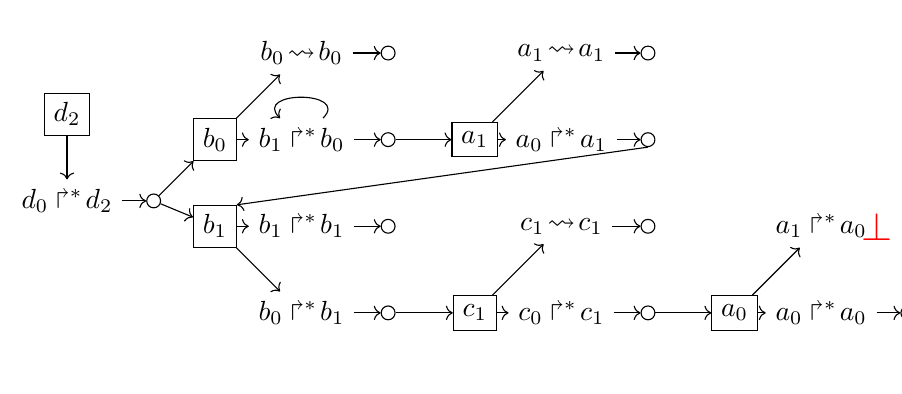
\begin{tikzpicture}[aS,node distance=1.1cm,shorthandon]
\path[use as bounding box] (-0.5,-2.1) rectangle (10.25,2.2);

\node[Aobj] (d02) {$\PHobjectif{d_0}{d_2}$};
\node[Aproc,above of=d02] (d2) {$d_2$};

\node[Asol,right of=d02] (d02s2) {};
\node[Aproc,above right of=d02s2] (b0) {$b_0$};
\node[Aobj,right of=b0] (b10) {$\PHobjectif{b_1}{b_0}$};
\node[Asol,right of=b10] (b10s) {};
\node[Aproc,right of=b10s] (a1) {$a_1$};
\node[Aobj,right of=a1] (a01) {$\PHobjectif{a_0}{a_1}$};
\node[Asol,right of=a01] (a01s) {};

\node[Aproc, below of=b0] (b1) {$b_1$};
\node[Aobj,right of=b1] (b11) {$\PHobjectif{b_1}{b_1}$};
\node[Asol,right of=b11] (b11s) {};
\node[Aobj,below of=b11] (b01) {$\PHobjectif{b_0}{b_1}$};
\node[Asol,right of=b01] (b01s) {};
\node[Aproc,right of=b01s] (c1) {$c_1$};
\node[Aobj,right of=c1] (c01) {$\PHobjectif{c_0}{c_1}$};
\node[Asol,right of=c01] (c01s) {};
\node[Aproc,right of=c01s] (a0) {$a_0$};
\node[Aobj,right of=a0] (a00) {$\PHobjectif{a_0}{a_0}$};
\node[Asol,right of=a00] (a00s) {};

\node[Aobj,above of=b10] (b00) {$\obj{b_0}{b_0}$};
\node[Asol,right of=b00] (b00s) {};
\node[Aobj,above of=a01] (a11) {$\obj{a_1}{a_1}$};
\node[Asol,right of=a11] (a11s) {};
\node[Aobj,above of=c01] (c11) {$\obj{c_1}{c_1}$};
\node[Asol,right of=c11] (c11s) {};
\node[Aobj,above of=a00] (a10) {$\PHobjectif{a_1}{a_0}$};
\node at (a10.east) {\Large\color{red}\textbf{$\bot$}};

\path
  (b10) edge[loop,min distance=5mm] (b10)
 ;
\path
(d02) edge (d02s2) (d02s2) edge (b1) edge (b0)
(a01) edge (a01s) (a01s.south) edge (b1.north east)
(b10) edge (b10s) (b10s) edge (a1)
(b11) edge (b11s)
(a1) edge (a01)
(b0) edge (b10) (b1) edge (b11)
(d2) edge (d02)
;
\path
(b00) edge (b00s)
(b0) edge (b00)
 (b1) edge (b01)
 (b01) edge (b01s) (b01s) edge (c1)
 (c1) edge (c01)
 (c01) edge (c01s) (c01s) edge (a0)
 (a0) edge (a00) (a00) edge (a00s)
;
\path
 (c1) edge (c11) (c11) edge (c11s)
(a0) edge (a10)
(a1) edge (a11)
(a11) edge (a11s)
;

%\node[right of=a01s] {\textbf{\Large\color{darkyellow}Inconc}};

\end{tikzpicture}%
}

% Structure abstraite / Sur-approximation / Non
\def \saono {%
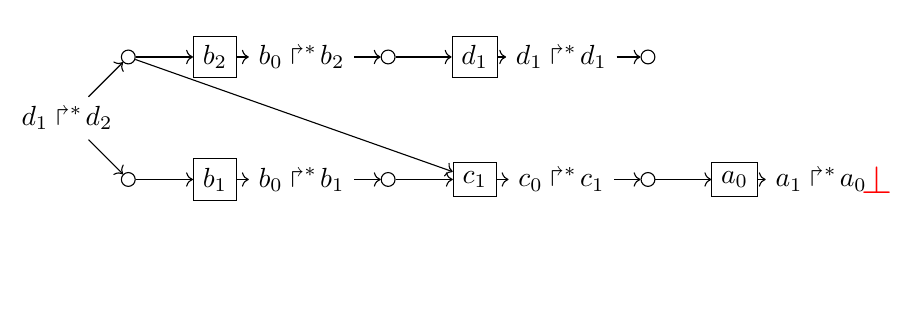
\begin{tikzpicture}[aS,node distance=1.1cm,shorthandon]
\path[use as bounding box] (-0.5,-2.1) rectangle (10.25,1.15);

\node[Aobj] (d12) {$\PHobjectif{d_1}{d_2}$};
\node[Asol,above right of=d12] (d12s1) {};
\node[Aproc, right of=d12s1] (b2) {$b_2$};
\node[Aobj,right of=b2] (b02) {$\PHobjectif{b_0}{b_2}$};
\node[Asol,right of=b02] (b02s) {};
\node[Aproc,right of=b02s] (d1) {$d_1$};
\node[Aobj,right of=d1] (d11) {$\PHobjectif{d_1}{d_1}$};
\node[Asol,right of=d11] (d11s) {};

\node[Asol,below right of=d12] (d12s2) {};
\node[Aproc, right of=d12s2] (b1) {$b_1$};
\node[Aobj,right of=b1] (b01) {$\PHobjectif{b_0}{b_1}$};
\node[Asol,right of=b01] (b01s) {};
\node[Aproc,right of=b01s] (c1) {$c_1$};
\node[Aobj,right of=c1] (c01) {$\PHobjectif{c_0}{c_1}$};
\node[Asol,right of=c01] (c01s) {};
\node[Aproc,right of=c01s] (a0) {$a_0$};
\node[Aobj,right of=a0] (a10) {$\PHobjectif{a_1}{a_0}$};
\node at (a10.east) {\Large\color{red}\textbf{$\bot$}};

\path
(d12) edge (d12s1) edge (d12s2) (d12s1) edge (b2) edge (c1) (d12s2) edge (b1)
(b01) edge (b01s) (b01s) edge (c1)
(b02) edge (b02s) (b02s) edge (d1)
(c01) edge (c01s) (c01s) edge (a0)
(d11) edge (d11s)
(a0) edge (a10)
(b1) edge (b01)
(b2) edge (b02)
(c1) edge (c01)
(d1) edge (d11)
;
%\only<\value{anim1}>{ \node[above right of=c01s] {\textbf{\Large\color{red}No}};}
\end{tikzpicture}%
}

% Structure abstraite / Sur-approximation / Inconclusif
\def \saoinconc {%
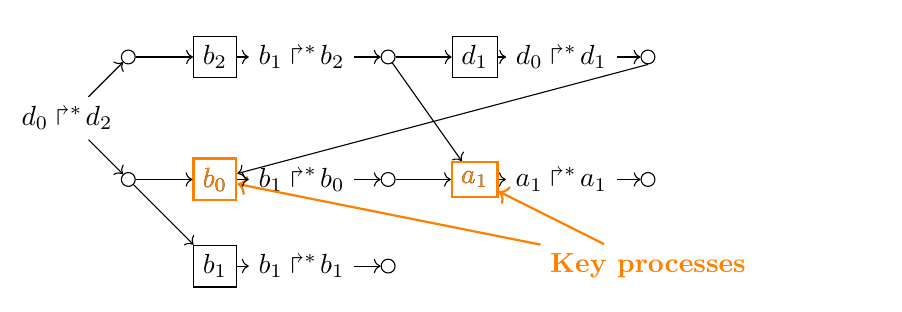
\begin{tikzpicture}[aS,node distance=1.1cm,shorthandon]
\path[use as bounding box] (-0.5,-2.1) rectangle (10.25,1.15);

\node[Aobj] (d02) {$\PHobjectif{d_0}{d_2}$};
\node[Asol,above right of=d02] (d02s1) {};

\node[Aproc, right of=d02s1] (b2) {$b_2$};
\node[Aobj,right of=b2] (b12) {$\PHobjectif{b_1}{b_2}$};
\node[Asol,right of=b12] (b12s) {};
\node[Aproc,right of=b12s] (d1) {$d_1$};
\node[Aobj,right of=d1] (d01) {$\PHobjectif{d_0}{d_1}$};
\node[Asol,right of=d01] (d01s) {};

\node[Asol,below right of=d02] (d02s2) {};
%<-3>
\node<-\tof>[Aproc, right of=d02s2] (b0) {$b_0$};
\node<\tokp>[orange, thick, Aproc, right of=d02s2] (b0) {$b_0$};
\node[Aobj,right of=b0] (b10) {$\PHobjectif{b_1}{b_0}$};
\node[Asol,right of=b10] (b10s) {};
%<-3>
\node<-\tof>[Aproc,right of=b10s] (a1) {$a_1$};
\node<\tokp>[orange, thick, Aproc,right of=b10s] (a1) {$a_1$};
\node[Aobj,right of=a1] (a11) {$\PHobjectif{a_1}{a_1}$};
\node[Asol,right of=a11] (a11s) {};

\node[Aproc, below of=b0] (b1) {$b_1$};
\node[Aobj,right of=b1] (b11) {$\PHobjectif{b_1}{b_1}$};
\node[Asol,right of=b11] (b11s) {};

\node<\tokp>[orange, font=\bfseries,below of=a11s] (kp) {Key processes};
\path<\tokp>[orange, thick]
        (kp) edge (a1)
        (kp) edge (b0)
;
\path
(d02) edge (d02s1) edge (d02s2) (d02s1) edge (b2) (d02s2) edge (b1) edge (b0)
(a11) edge (a11s)
(b10) edge (b10s) (b10s) edge (a1)
(b11) edge (b11s)
(b12) edge (b12s) (b12s) edge (d1) edge (a1)
(d01) edge (d01s) (d01s.south) edge (b0)
(a1) edge (a11)
(b0) edge (b10) (b1) edge (b11) (b2) edge (b12)
(d1) edge (d01)
;
%\node[below right of=d01s] {\textbf{\Large\color{yellow}Inconc}};
\end{tikzpicture}%
}


\def \sasaquant {

    \begin{tikzpicture}[aS,node distance=1.1cm,shorthandon]
    
    % \path[use as bounding box] (-0.5,-3.1) rectangle (10.25,1.15);
     \path[use as bounding box] (3,0) rectangle (10.25,-2.15);

      \node[Aproc] (d2) {$d_2$};
      \node[Aobj,below of=d2] (d12) {$\PHobjectif{d_1}{d_2}{\color{blue}(0.14)}$};
      \node[Asol,right of=d12] (d12s) {};
      

      \node[Aproc,right of=d12s] (bbs) {$b_1,bs_1,\rlab{e_1}$};
      \node[Asol,right of=bbs] (bbss) {};

      \node[Aproc,right  of=bbss] (b1) {$b_1$};
      \node[Aobj,right of=b1] (b01) {$\PHobjectif{b_0}{b_1}{\color{blue}(0.05)}$};
      \node[Asol,right of=b01] (b01s) {};
      %\node[Aobj,below left of=a1] (a01) {$\PHobj{a_0}{a_1}$};
      %\node[Asol,below of=a01] (a01s) {};
      \node[Aproc,right of=b01s] (a1) {$\rlab{c_1},a_1$};
      \node[Aobj,right of=a1] (a11) {$\PHobjectif{a_1}{a_1}{\color{blue}(1)}$};
      \node[Asol,right of=a11] (a11s) {};
      \node[RAobj,above right of=a1] (c11) {$\PHobjectif{c_1}{c_1}{\color{blue}(1)}$};
      \node[RAsol,right of=c11] (c11s) {{\Large\color{red}\textbf{$\otimes$}}};
      %\node[Aobj,below left of=b0] (b10) {$\PHobj{b_1}{b_0}$};
      %\node[Asol,below of=b10] (b10s) {};

      \node[Aproc,below right  of=bbss] (bs1) {$bs_1$};
      \node[Aobj,right of=bs1] (bs01) {$\PHobjectif{bs_0}{bs_1}{\color{blue}(1)}$};
      \node[Asol,right of=bs01] (bs01s) {};
      %\node[Aobj,below right of=b1] (b01) {$\PHobj{b_0}{b_1}$};
      %\node[Asol,below of=b01] (b01s) {};
      \node[Aproc,right of=bs01s] (as1) {$a_1$};
      \node[Aobj,right of=as1] (as11) {$\PHobjectif{a_1}{a_1}{\color{blue}(1)}$};
      \node[Asol,right of=as11] (as11s) {};
      %\node[Aobj,below right of=a0] (a10) {$\PHobj{a_1}{a_0}$};
      %\node[Asol,below of=a10] (a10s) {};

      \node[RAproc,above right of=bbss] (e1) {$e_1$};
      \node[RAobj,right of=e1] (e01) {$\PHobjectif{e_0}{e_1}{\color{blue}(1)}$};
      \node[RAsol,right of=e01] (e01s) {{\Large\color{red}\textbf{$\otimes$}}};

      \path
      (d2) edge (d12)
      (d12) edge (d12s)
      (d12s) edge (bbs)
      (bbs) edge (bbss)
      (bbss) edge (bs1) edge (b1) edge[red] (e1)

      (b1) edge (b01) 
      (b01) edge (b01s)
      (b01s) edge (a1)
      (a1) edge (a11)
      (a11) edge (a11s)
      (a1) edge[red] (c11)
      (c11) edge[red] (c11s)
      %(a0) edge (a10) edge (a00)
      %(a10) edge (a10s)
      %(a00) edge (a00s)

      (bs1) edge (bs01) 
      (bs01) edge (bs01s)
      (bs01s) edge (as1)
      (as1) edge (as11)
      (as11) edge (as11s) 
      %(b01) edge (b01s)
      %(b01s) edge (a0)
      %(b11) edge (b11s)

      (e1) edge[red] (e01) 
      (e01) edge[red] (e01s)
      ;
      \end{tikzpicture}


}

%%% Exemple pour la définition des an %%%
\def \exandef {
\path[use as bounding box] (-0.5,-0.5) rectangle (6.5,4.5);

\TSort{(0,1)}{a}{3}{l}
\TSort{(3,1)}{b}{2}{l}
\TSort{(6,1)}{c}{3}{l}

\path[local transitions]
  (a_0) edge node[auto] {$b_0$} (a_1)
  (a_1) edge (a_0)
  (a_0) edge[bend right=60] node[right] {$b_0,c_0$} (a_2)
  (c_0) edge node[auto] {$a_1$} (c_1)
  (c_1) edge node[auto] {$b_0$} (c_2)
  (c_1) edge node[auto] {$b_1$} (c_0)
  (b_0) edge (b_1)
  (b_1) edge node[auto] {$a_0$} (b_0)
;
}

%%% Exemple pour la définition des an %%%
\def \exanaspdef {
\path[use as bounding box] (-0.5,-0.5) rectangle (6.5,4.5);

\TSort{(3,1.5)}{a}{3}{l}

\path[local transitions]
  (a_0) edge node[auto] {$b_0$} (a_1)
  (a_1) edge (a_0)
  (a_0) edge[bend right=60] node[right] {$b_0,c_0$} (a_2)
;
}

%%% Exemple pour la définition des san %%%
\def \exsandef {
\path[use as bounding box] (-0.5,-0.5) rectangle (6.5,4.5);

\TSort{(0,1)}{a}{3}{l}
\TSort{(3,1)}{b}{2}{l}
\TSort{(6,1)}{c}{3}{l}

\path[local transitions]
  (a_0) edge node[auto] {$b_0,\mathbf{\color{Maroon} 2}$} (a_1)
  (a_1) edge node[auto] {$\mathbf{\color{Maroon} 1}$} (a_0)
  (a_0) edge[bend right=60] node[right] {$b_0,c_0,\mathbf{\color{Maroon} 2}$} (a_2)
  (c_0) edge node[auto] {$a_1,\mathbf{\color{Maroon} 3}$} (c_1)
  (c_1) edge node[auto] {$b_0,\mathbf{\color{Maroon} 2}$} (c_2)
  (c_1) edge node[auto] {$b_1,\mathbf{\color{Maroon} 1}$} (c_0)
  (b_0) edge node[auto] {$\mathbf{\color{Maroon} 3}$}(b_1)
  (b_1) edge node[auto] {$a_0,\mathbf{\color{Maroon} 1}$} (b_0)
;
}

%%% Exemple pour l'interpretation abstraite %%%
\def \exanaidef {
\path[use as bounding box] (-0.5,-0.5) rectangle (6.5,4.5);

\TSort{(3,1.5)}{d}{3}{l}

\path[local transitions]
  (d_1) edge[bend right] node[right] {$c_2$} (d_2)
  (d_1) edge node[auto] {$b_1$} (d_2)
  (d_1) edge node[auto] {$e_1$} (d_0)
;
}

%le GLC associé
\def \exlcgaidef {

    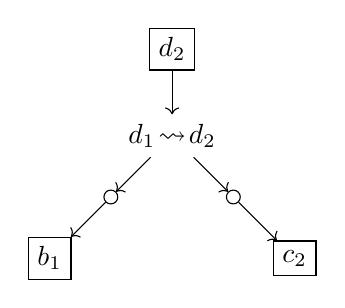
\begin{tikzpicture}[aS,node distance=1.1cm,shorthandon]
    
    %\path[use as bounding box] (-0.5,-0.5) rectangle (6.5,4.5);
    %les noeuds
    \node[Aproc] (d2) {$d_2$};
    \node[Aobj,below of=d2] (d12) {$\obj{d_1}{d_2}$};
    \node[Asol,below left of=d12] (d12s1) {};
    \node[Asol,below right of=d12] (d12s2) {};

    \node[Aproc, below right of=d12s2] (c2) {$c_2$};
    \node[Aproc, below left of=d12s1] (b1) {$b_1$};
    %\node[Aproc, below right of=a02s2] (b0) {$b_0$};
    
    

    \path
      (d2) edge (d12)
      (d12) edge (d12s1)
      (d12) edge (d12s2)
      (d12s1) edge (b1)
      (d12s2) edge (c2)
;
\end{tikzpicture}
} 


%%% Exemple pour l'interpretation abstraite quantifié%%%
\def \exsanaidef {
\path[use as bounding box] (1.5,-0.5) rectangle (3.5,3.5);

\TSort{(3,1.5)}{d}{3}{l}

\path[local transitions]
  (d_1) edge[bend right] node[right] {$c_2,\mathbf{\color{Maroon} 2}$} (d_2)
  (d_1) edge node[auto] {$b_1,\mathbf{\color{Maroon} 3}$} (d_2)
  (d_1) edge[red] node[auto] {${\color{red}e_1},\mathbf{\color{Maroon} 2}$} (d_0)
;
}

%le QGLC associé
\def \exqlcgaidef {

    \begin{tikzpicture}[aS,node distance=1.1cm,shorthandon]
    
    %\path[use as bounding box] (0,-3) rectangle (2,1);
    %les noeuds
    \node[Aproc] (d2) {$d_2$};
    \node[Aobj,below of=d2] (d12) {$\obj{d_1}{d_2}$};
    \node[Asol,below left of=d12] (d12s1) {};
    \node[Asol,below right of=d12] (d12s2) {};
    \node[Asol, right of=d12,red] (d12s3) {};

    \node[Aproc, below right of=d12s2] (c2) {$c_2$};
    \node[Aproc, below left of=d12s1] (b1) {$b_1$};
    %solution conccurente
    \node[Aproc, right of=d12s3,red] (e1) {$e_1$};
   
   
    \node[labelproba, right of=d2,node distance=1.8cm] (pd2) {${\color{blue}\{\Prob{d_2},\Time{d_2}\}}$};
    \node[labelproba, left of=d12,node distance=2.8cm] (pd12) {${\color{blue}\{\Prob{\obj{d_1}{d_2}},\Time{\obj{d_1}{d_2}}\}}$};
    \node[labelproba, left of=b1,node distance=1.5cm] (pb1) {${\color{blue}\{\Prob{b_1},\Time{b_1}\}}$};
    \node[labelproba, right of=c2,node distance=1.5cm] (pc2) {${\color{blue}\{\Prob{c_2},\Time{c_2}\}}$};
    \node[labelproba, below of=e1,node distance=0.5cm] (pe1) {${\color{red}\{\Prob{e_1},\Time{e_1}\}}$};
    
    \path
      (d2) edge (d12)
      (d12) edge (d12s1)
      (d12) edge (d12s2)
      (d12) edge[red] (d12s3)
      (d12s1) edge (b1)
      (d12s2) edge (c2)
      (d12s3) edge[red] (e1)
      
;
\end{tikzpicture}
} 

%le QGLC généralisé
\def \exqlcggaidef {

    \begin{tikzpicture}[aS,node distance=1.1cm,shorthandon]
    
    \path[use as bounding box] (0,-3) rectangle (2,1);
    %les noeuds
    \node[Aproc] (d2) {$\n_k$};
    \node[Aobj,below of=d2] (d12) {$obj_k$};
    \node[Asol,below left of=d12] (d12s1) {};
    \node[Asol,below right of=d12] (d12s2) {};

    \node[Aproc, below right of=d12s2] (c2) {$\n_{k-1,2}$};
    \node[Aproc, below left of=d12s1] (b1) {$\n_{k-1,1}$};
    %\node[Aproc, below right of=a02s2] (b0) {$b_0$};
    \node[labelproba, right of=d2,node distance=1.8cm] (pd2) {${\color{blue}\{\Prob{\n_k},\Time{\n_k}\}}$};
    \node[labelproba, right of=d12,node distance=1.8cm] (pd12) {${\color{blue}\{\Prob{obj_k},\Time{obj_k}\}}$};
    \node[labelproba, left of=b1,node distance=2.4cm] (pb1) {${\color{blue}\{\Prob{\n_{k-1,1}},\Time{\n_{k-1,1}}\}}$};
    \node[labelproba, right of=c2,node distance=2.3cm] (pc2) {${\color{blue}\{\Prob{\n_{k-1,2}},\Time{\n_{k-1,2}}\}}$};
    
    
    \path
      (d2) edge (d12)
      (d12) edge (d12s1)
      (d12) edge (d12s2)
      (d12s1) edge (b1)
      (d12s2) edge (c2)
;
\end{tikzpicture}
} 



%exemple d'un an pour annoncer les san et le glc quantifié
\def \exanppdef {
%\path[use as bounding box] (-0.5,-0.5) rectangle (10.5,17.5);

\TSort{(0,1)}{a}{2}{l}
\TSort{(2.5,1)}{b}{2}{l}
\TSort{(2.5,4)}{c}{3}{l}
\TSort{(0,4)}{d}{3}{l}
\TSort{(2.5,8)}{e}{2}{l}
\TSort{(0,8)}{f}{2}{l}
%\TState{a_0,b_0,c_1,d_1,e_1,f_0}

\path[local transitions]
  (a_0) edge (a_1)
  (a_1) edge node[auto] {$c_2$}(a_0)
  (c_0) edge node[auto] {$f_0$} (c_1)
  (c_1) edge node[auto] {$f_0$} (c_2)
  (c_1) edge node[auto] {$f_1$} (c_0)
  (b_0) edge node[auto] {$a_1$}(b_1)
  (b_1) edge node[auto] {$a_0$} (b_0)
  (d_1) edge[bend right] node[right] {$c_2$} (d_2)
  (d_1) edge node[auto] {$b_1$} (d_2)
  (d_1) edge node[auto] {$e_1$} (d_0)
  (e_0) edge node[auto] {$d_0$} (e_1)
  (e_1) edge node[auto] {$d_2$} (e_0)
  (f_0) edge (f_1)
  (f_1) edge node[auto] {$b_1$} (f_0)
;
}

\def \exglcandef {

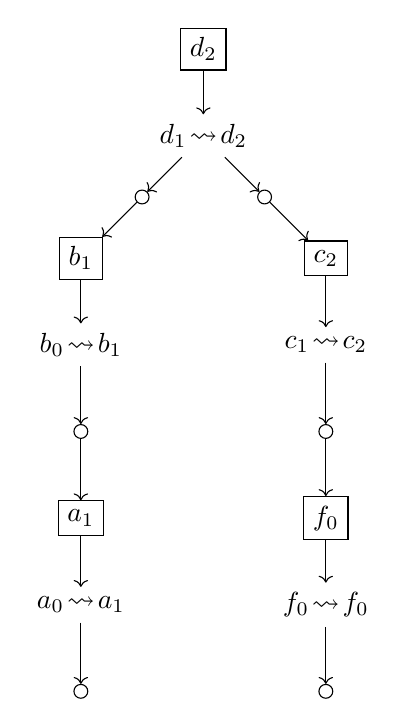
\begin{tikzpicture}[aS,node distance=1.1cm,shorthandon]
    
    %\path[use as bounding box] (0,-1) rectangle (2,1);
    %les noeuds
    \node[Aproc] (a2) {$d_2$};
    \node[Aobj,below of=a2] (a02) {$\obj{d_1}{d_2}$};
    \node[Asol,below left of=a02] (a02s1) {};
    \node[Asol,below right of=a02] (a02s2) {};

    \node[Aproc, below right of=a02s2] (c2) {$c_2$};
    \node[Aproc, below left of=a02s1] (b1) {$b_1$};
    
    \node[Aobj,below of=b1] (b01) {$\obj{b_0}{b_1}$};
    \node[Asol,below of=b01] (b01s) {};
    \node[Aproc,below of=b01s] (a1) {$a_1$};
    \node[Aobj,below of=a1] (a01) {$\obj{a_0}{a_1}$};
    \node[Asol,below of=a01] (a01s) {};
    
    
    \node[Aobj,below of=c2] (c12) {$\obj{c_1}{c_2}$};
    \node[Asol,below of=c12] (c12s) {};
    \node[Aproc,below of=c12s] (f0) {$f_0$};
    \node[Aobj,below of=f0] (f00) {$\obj{f_0}{f_0}$};
    \node[Asol,below of=f00] (f00s) {};
    

    \path
      (a2) edge (a02)
      (a02) edge (a02s1)
      (a02) edge (a02s2)
      (a02s1) edge (b1)
      (a02s2) edge (c2)
      (c2) edge (c12)
      (c12) edge (c12s)
      (c12s) edge (f0)
      (f0) edge (f00)
      (f00) edge (f00s)
      (b1) edge (b01)
      (b01) edge (b01s)
      (b01s) edge (a1)
      (a1) edge (a01)
      (a01) edge (a01s)
;
\end{tikzpicture}
}




%exemple d'un san pour illustrer le glc quantifié

\def \exsanppdef {
%\path[use as bounding box] (-0.5,-0.5) rectangle (10.5,17.5);

\TSort{(0,1)}{a}{2}{l}
\TSort{(2.5,1)}{b}{2}{l}
\TSort{(2.5,4)}{c}{3}{l}
\TSort{(0,4)}{d}{3}{l}
\TSort{(2.5,8)}{e}{2}{l}
\TSort{(0,8)}{f}{2}{l}


\path[local transitions]
  (a_0) edge node[auto] {$\mathbf{\color{Maroon} 2}$} (a_1)
  (a_1) edge node[auto] {$c_2,\mathbf{\color{Maroon} 1}$} (a_0)
  (c_0) edge node[auto] {$f_0,\mathbf{\color{Maroon} 2}$} (c_1)
  (c_1) edge node[auto] {$f_0,\mathbf{\color{Maroon} 2}$} (c_2)
  (c_1) edge node[auto] {$f_1,\mathbf{\color{Maroon} 1}$} (c_0)
  (b_0) edge node[auto] {$a_1,\mathbf{\color{Maroon} 2}$}(b_1)
  (b_1) edge node[auto] {$a_0,\mathbf{\color{Maroon} 1}$} (b_0)
  (d_1) edge[bend right] node[right] {$c_2,\mathbf{\color{Maroon} 2}$} (d_2)
  (d_1) edge node[auto] {$b_1,\mathbf{\color{Maroon} 3}$} (d_2)
  (d_1) edge node[auto] {$e_1,\mathbf{\color{Maroon} 2}$} (d_0)
  (e_0) edge node[auto] {$d_0,\mathbf{\color{Maroon} 2}$} (e_1)
  (e_1) edge node[auto] {$d_2,\mathbf{\color{Maroon} 1}$} (e_0)
  (f_0) edge node[auto] {\mathbf{\color{Maroon} 2}}(f_1)
  (f_1) edge node[auto] {$b_1,\mathbf{\color{Maroon} 1}$} (f_0)
;
}

%exemple de GLC quantifié 
\def \exglcsandef {

\begin{tikzpicture}[aS,node distance=1.1cm,shorthandon]
    
    %\path[use as bounding box] (0,-1) rectangle (2,1);
    %les noeuds
    \node[Aproc] (a2) {$d_2$};
    \node[Aobj,below of=a2] (a02) {$\obj{d_1}{d_2}$};
    \node[Asol,below left of=a02] (a02s1) {};
    \node[Asol,below right of=a02] (a02s2) {};

    \node[Aproc, below right of=a02s2] (c2) {$c_2$};
    \node[Aproc, below left of=a02s1] (b1) {$b_1$};
    
    \node[Aobj,below of=b1] (b01) {$\obj{b_0}{b_1}$};
    \node[Asol,below of=b01] (b01s) {};
    \node[Aproc,below of=b01s] (a1) {$a_1$};
    \node[Aobj,below of=a1] (a01) {$\obj{a_0}{a_1}$};
    \node[Asol,below of=a01] (a01s) {};
    
    
    \node[Aobj,below of=c2] (c12) {$\obj{c_1}{c_2}$};
    \node[Asol,below of=c12] (c12s) {};
    \node[Aproc,below of=c12s] (f0) {$f_0$};
    \node[Aobj,below of=f0] (f00) {$\obj{f_0}{f_0}$};
    \node[Asol,below of=f00] (f00s) {};
    
    %node label pour les probas
    \node[labelproba1, right of=d2,node distance=1.1cm] (pd2) {${\color{blue}\{\frac{13}{19}\}}$};
    \node[labelproba2, right of=d12,node distance=1.1cm] (pd12) {${\color{blue}\{\frac{13}{19}\}}$};
    \node[labelproba3, left of=b1,node distance=1.1cm] (pb1) {${\color{blue}\{1\}}$};
    \node[labelproba4, right of=c2,node distance=1.1cm] (pc2) {${\color{blue}\{\frac{2}{3}\}}$};
    \node[labelproba5, left of=b01,node distance=1.1cm] (pb01) {${\color{blue}\{1\}}$};
    \node[labelproba6, right of=c12,node distance=1.1cm] (pc12) {${\color{blue}\{\frac{2}{3}\}}$};
    \node[labelproba7, left of=a1,node distance=1.1cm] (pa1) {${\color{blue}\{1\}}$};
    \node[labelproba8, right of=f0,node distance=1.1cm] (pf0) {${\color{blue}\{1\}}$};
    \node[labelproba9, left of=a01,node distance=1.1cm] (pa01) {${\color{blue}\{1\}}$};
    \node[labelproba10, right of=f00,node distance=1.1cm] (pf00) {${\color{blue}\{1\}}$};
    \node[labelproba11, left of=a01s,node distance=1.1cm] (pa01s) {${\color{blue}\{1\}}$};
    \node[labelproba12, right of=f00s,node distance=1.1cm] (pf00s) {${\color{blue}\{1\}}$};
    
    \path
      (a2) edge (a02)
      (a02) edge (a02s1)
      (a02) edge (a02s2)
      (a02s1) edge (b1)
      (a02s2) edge (c2)
      (c2) edge (c12)
      (c12) edge (c12s)
      (c12s) edge (f0)
      (f0) edge (f00)
      (f00) edge (f00s)
      (b1) edge (b01)
      (b01) edge (b01s)
      (b01s) edge (a1)
      (a1) edge (a01)
      (a01) edge (a01s)
;
\end{tikzpicture}
}

% Légende pour les GLC
\newcommand{\lvalign}{1 cm}
\newcommand{\lhfirst}{3 cm}
\newcommand{\lhsep}{.7 cm}
%\newcommand{\lvin}{.2}
%\newcommand{\lvout}{1.8}
\newcommand{\lvalignl}{2.2 cm}
\tikzstyle {llegend}=[anchor=west,align=left]
\tikzstyle {legendbox}=[rounded corners,thick,draw=couleurtheme]

\def \glclegend#1#2#3{
  \node[cplx] at (\lvalign,\lhfirst) (excplx) {#2};
  \node[qgre] at (\lvalign,\lhfirst-\lhsep) (exgene) {#1};
  \node[sn] at (\lvalign,\lhfirst-2*\lhsep) (exsn) {#3};
  \node[mod] at (\lvalign,\lhfirst-3*\lhsep) (extrans) {};

  \node[llegend] at (\lvalignl,\lhfirst) {Complexe, protéine};
  \node[llegend] at (\lvalignl,\lhfirst-\lhsep) {gène};
  \node[llegend] at (\lvalignl,\lhfirst-2*\lhsep) {état cellulaire};
  \node[llegend] at (\lvalignl,\lhfirst-3*\lhsep) {n{\oe}ud transitoire};

  \ifthenelse{\equal{#1}{prio}}{%
%     \node[Aproc] at (\lvalign-.3cm,\lhfirst-3*\lhsep) (aprio1) {$ab_{11}$};
%     \node[Asol] at (\lvalign+.7cm,\lhfirst-3*\lhsep) (aprio2) {};
%     \path (aprio1) edge[aSPrio] (aprio2);
    \node[Async] at (\lvalign,\lhfirst-3*\lhsep) (aprio1) {$\{a_1, b_1\}$};
    \node[llegend] at (\lvalignl,\lhfirst-3*\lhsep) {\phantom{Mg}\\Synchronization of\\several processes};
    \path[legendbox] (0,0) rectangle (5.8,3.6);
  }{%
    \path[legendbox] (0,0.5) rectangle (5.8,3.6);
  }
}





%%% Citations
\newcommand{\citeegfra}{\quad\tval{\ex{egfr20}}: \tcite{Epidermal Growth Factor Receptor, by Özgür Sahin \textit{et al.}}}
\newcommand{\citeegfrb}{\quad\tval{\ex{egfr104}}: \tcite{Epidermal Growth Factor Receptor, by Regina Samaga \textit{et al.}}}
\newcommand{\citetcrsiga}{\quad\tval{\ex{tcrsig40}}: \tcite{T-Cell Receptor Signaling, by Steffen Klamt \textit{et al.}}}
\newcommand{\citetcrsigb}{\quad\tval{\ex{tcrsig94}}: \tcite{T-Cell Receptor Signaling, by Julio Saez-Rodriguez \textit{et al.}}}

\newcommand{\citemodels}{\bigskip\citeegfra\\\citeegfrb\\\citetcrsiga\\\citetcrsigb}

\newcommand{\citepmrtcsb}{Paulevé, Magnin, Roux in \textit{Transactions on Computational Systems Biology}, 2011}
\newcommand{\citepmrmscs}{Paulevé, Magnin, Roux in \textit{Mathematical Structures in Computer Science}, 2012}
\newcommand{\citefpimrcmsb}{{\small Folschette, Paulevé, Inoue, Magnin, Roux\\in \textit{Computational Methods in Systems Biology}, 2012}}
%\newcommand{\crcbmfma}{Richard, Comet, Bernot in Modern Formal Methods and App., 2006}
\newcommand{\citedejong}{De Jong in \textit{Journal of Computational Biology}, 2002}
\newcommand{\citerichardcomet}{Richard, Comet in \textit{Discrete Applied Mathematics}, 2007}
\newcommand{\citeremy}{Remy, Ruet, Thieffry in \textit{Advances in Applied Mathematics}, 2008}
\newcommand{\citesmbionet}{Bernot, Comet, Richard, Guespin in \textit{Journal of Theoretical Biology}, 2004}
\newcommand{\citeito}{Ito, Izumi, Hagihara, Yonezaki in \textit{BioInformatics and BioEngineering}, 2010}
\newcommand{\citeatfb}{Abou-Jaoudé et al, in \textit{Frontiers in Bioengineering and Biotechnology}, 2015}
\newcommand{\citelui}{Liu et al, in \textit{Journal of Bioinformatics and Computational Biology}, 2012}
\newcommand{\citethomas}{Thomas, \textit{Journal of Theoretical Biology}, 1973}
\newcommand{\citekauffman}{Kauffman, \textit{Journal of Theoretical Biology}, 1969}
\newcommand{\citestocha}{Heiner, Priami, Phillips, etc.}
\newcommand{\citetemp}{Ahmad, Bockmayr,Paulev\'e}
\newcommand{\citecaritofebs}{Guziolowski et al, in \textit{Febs Journal},2012}
\newcommand{\citekolly}{Kolly et al, in \textit{J. Invest. Dermatol.},2005}
\newcommand{\citetu}{Tu et al, in \textit{J. Invest. Dermatol.},2011}
\newcommand{\citedata}{Peter Angel, Christian Schuster, \textit{DKFZ}}

%%slides en anglais

%%%%%%%%%     introduction
%\section{Introduction}
%% Diapo d'intro
\begin{frame}[c]
  \frametitle{Context}
%rajouter le titre (version courte) dans toute les slides
\begin{center}
  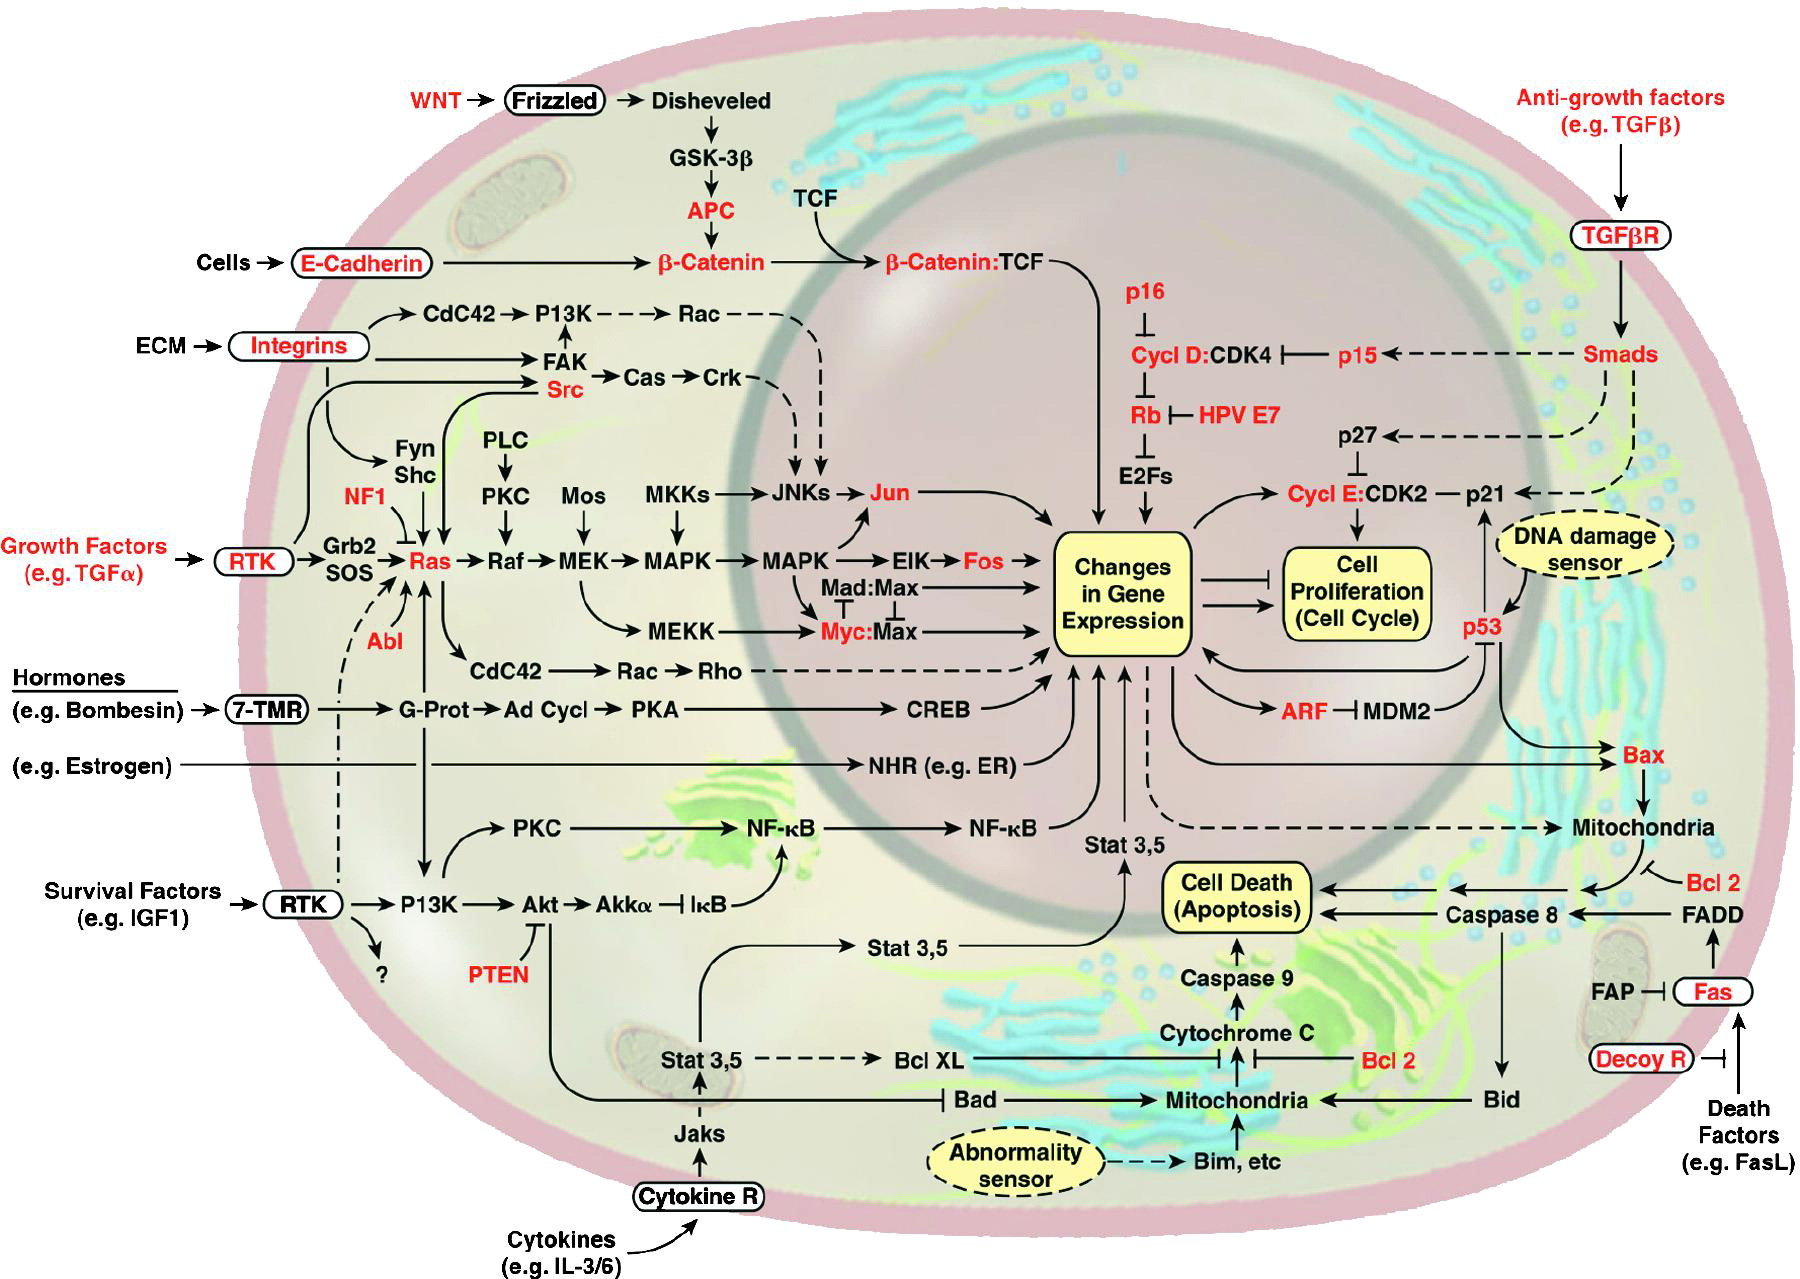
\includegraphics[scale=0.12]{images/cellule-description.jpeg}
\end{center}
\begin{center}
{\tiny \color{darkgreen}[\citelui]}
\end{center}

%\tcite{Wikipédia}

\begin{itemize}
\item Cellular processes are driven by networks of biological interactions.
\item Formal modelling and analysis of Biological Regulatory Network.
\item Static analysis of qualitative and quantitative properties.
\end{itemize}

%Cellular processes are driven by networks of biological reactions. Cells rely on the tight coordination of these pathways to achieve proper functioning.
%With the help of signaling pathway, a cell senses changes in its environnement or internal state. This information is then passed on via cascades of biochemical 
%reactions to the appropriate mechanisms which respond by modifying the metabolic and transcriptiona activities. this in turn modifies the behavior of the cell.

%Consequently, the dynamics of biopathways play a crucial role in determinig cellular functions.

%Examples: circadian rhythm, the apoptosis pathway inducing programmed cell death, cell differentiation.

%\textcolor{couleurtheme}{$\Rightarrow$} \fbox{\tval{\large The need of comprehension of biological systems}} \textcolor{couleurtheme}{$\Leftarrow$}


%\textcolor{couleurtheme}{$\Rightarrow$} \fbox{\tval{\large Allow efficient translation from Process Hitting to BRN}} \textcolor{couleurtheme}{$\Leftarrow$}

\end{frame}



%\begin{frame}
\frametitle{Biological Regulatory Networks Modelling \& Analysis}

\end{frame}

%\input{parts/position.tex}

%%\tableofcontents

%%\input{parts/static_analysis.tex}

%\section{Dynamics refinement by Time Series Data Integrating}
%
\begin{frame}[c]
 \frametitle{Motivation}
  %\pause
 %figure illustrative
 \begin{tikzpicture}[auto]
  
\path[use as bounding box] (-0.7,-2) rectangle (3,3);

%le noeud pour les connaissances de la littérature, générales
\node[align=center] (gk) at (2,3) {\begin{tabular}{|c|} 
\hline
 General knowledge  \\
 \hline
 Literature  \\
  \hline
 Hypotheses   \\
  \hline
\end{tabular}};

%\pause

%les noeud pour le réseau biologique
\node[qgre] (a) at (1,1.5) {a};
\node[mod] (i) at (2,1) {i};
\node[qgre] (b) at (1,0.5) {b};
\node[qgre] (c) at (2.5,1) {c};


\path
 (a) edge[act] (i)
 (b) edge[inh] (i)
 (i) edge[st]  (c);
 
 %\pause

\node (deco) at (2,-0.1) {Times series data};
\node[align=center] (tsd) at (2,-1) {\begin{tabular}{|c|c|c|c|} 
\hline
 Genes  & 1h & ... & 24h  \\
 \hline
 Gene $1$  &   & ...  &    \\
  \hline
  Gene $2$  &   & ...  &    \\
  \hline
\end{tabular}};


\onslide<2->{

\node (d1) at (5,1) {};
\node (d2) at (7.5,1) {};

\node (d3) at (4.5,-1.5) {};
\node (d4) at (4.5,3.5) {};


\draw[->,line width=6pt, color=lightgray] (d1) -- (d2) node[above=10pt,midway]{\textcolor{black}{\textbf{Algebraic Modelling}}};
}



%\draw[decoration={brace,amplitude=12pt}, 
%decorate,line width=2pt,gray] (d3) -- (d4) node[above=10pt,midway]{\textcolor{black}{\textbf{}}};


\onslide<3->{
%le modèle en process hitting
\node[scale=0.4] (phmodel) at (10,1) {\begin{tikzpicture} \exphHM 
                           \end{tikzpicture}};
}

\end{tikzpicture}

\onslide<2->{
 \begin{block}
  
  \begin{itemize}
   \item Formal characterisation of topology and dynamics of biological regulatory networks.
   \item Time-series data integration.
   \item Qualitative \& Quantitative refinement of the dynamics.        
   \item Stochastic simulation and statistic analysis.
  \end{itemize}

 \end{block}
}

\end{frame}

%\subsection{Biological Networks}
%\begin{frame}[c]
 \frametitle{RSTC Network}
 \framesubtitle{multi-layer receptor-signaling-transcription-cell state}
%\begin{beamer}

\begin{center}
  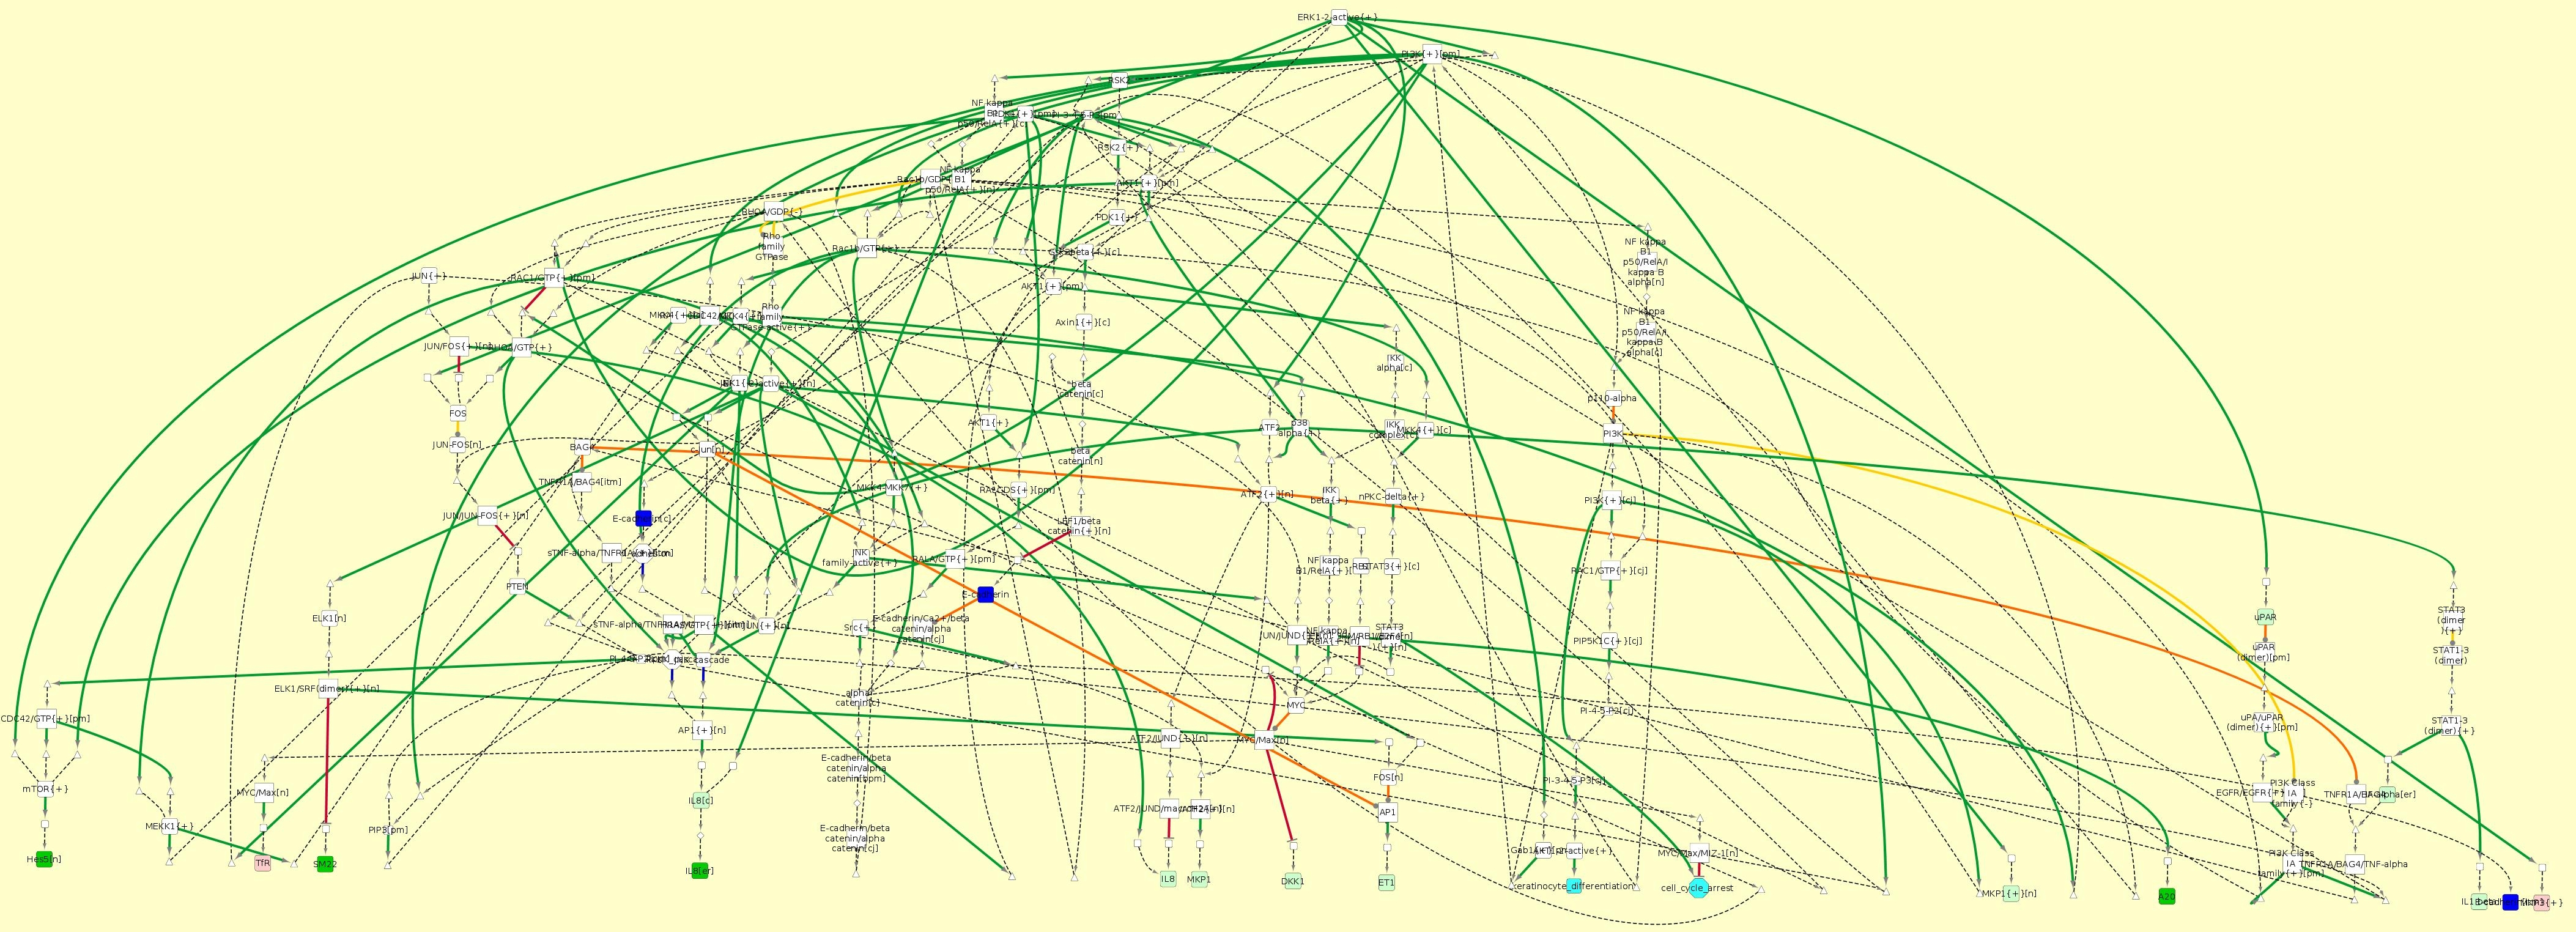
\includegraphics[scale=0.07]{figs/net.jpg}
\end{center}
 
%\end{beamer}

%\pause

\begin{itemize}
 \item Pathway Interaction Database
 \item \tval{$293$  nodes}: signaling proteins, transcription factors, mRNA expressions
 \item \tval{$375$  interactions}: activations, inhibitions, complexes dissociation
\end{itemize}

 
\end{frame}

\begin{frame}[c]
 \frametitle{RSTC Network}
 \framesubtitle{multi-layer receptor-signaling-transcription-cell state}

%%%image zoomée
\begin{tikzpicture}[node distance = 1em,dashed,red,thick]
	\zoomZero{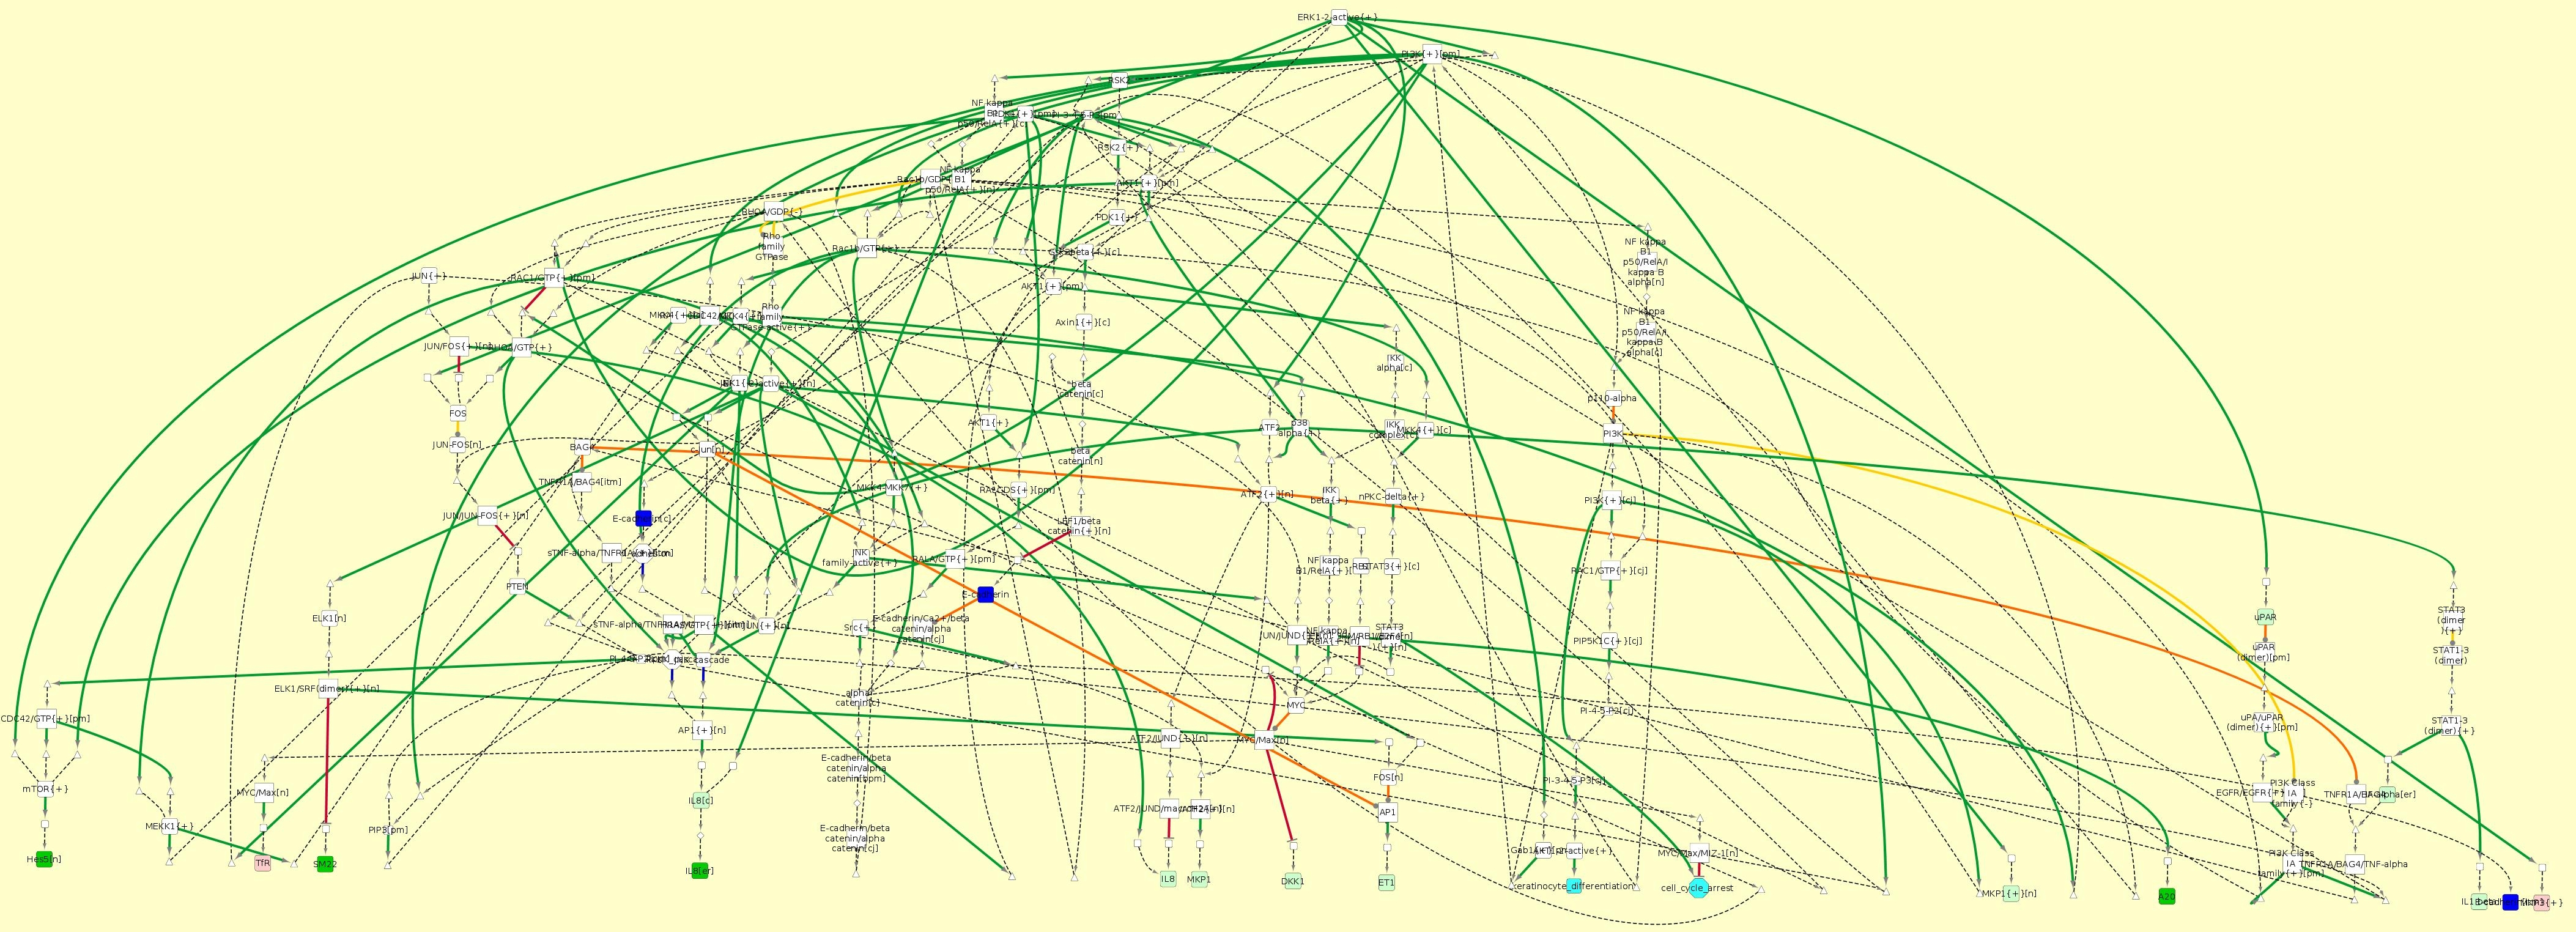
\includegraphics[width=0.35\textwidth]{figs/net.jpg}}
	\zoomIn[right]{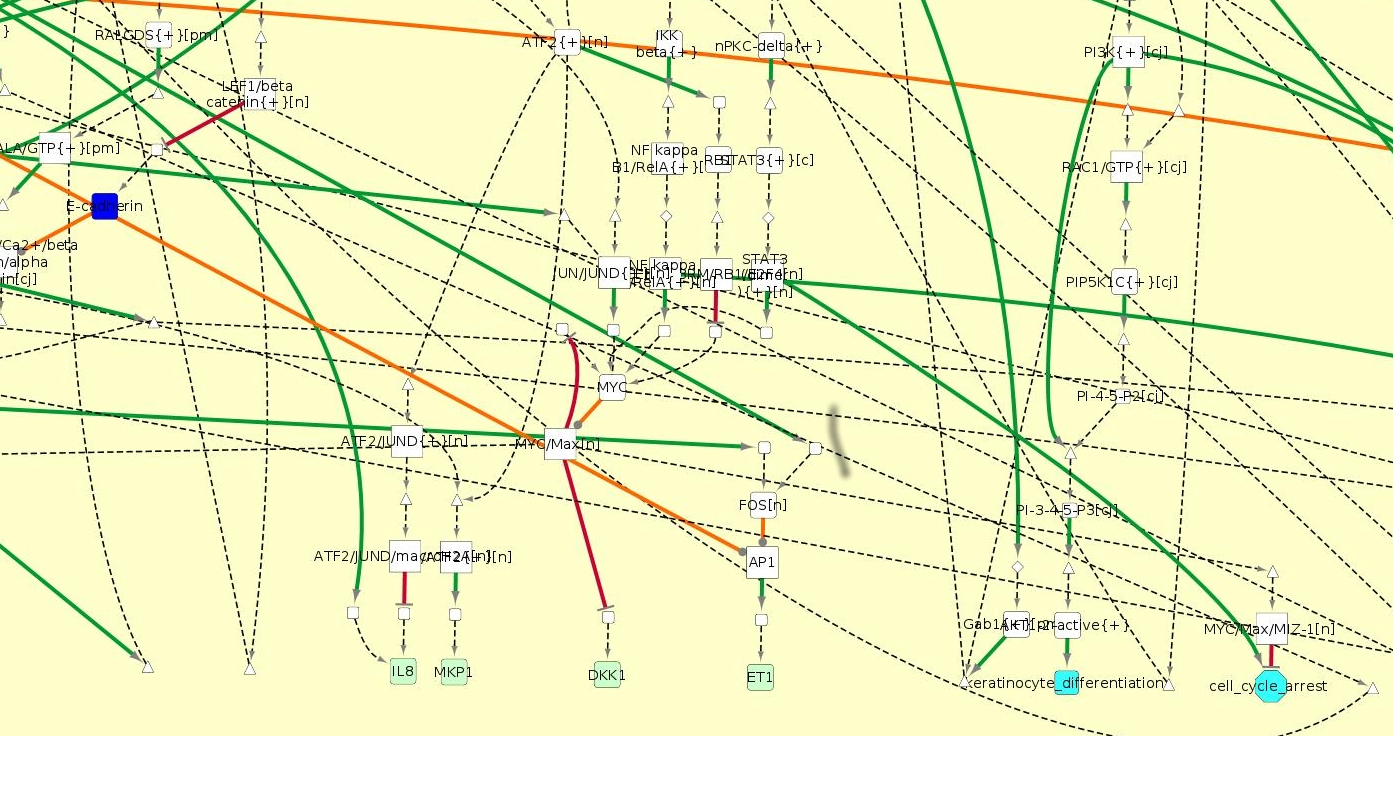
\includegraphics[scale=0.15]{figs/netzoom.png}}{0.35,0.005}{0.320,0.420}
	%\zoomIn{\includegraphics[width=0.45\textwidth]{Geant3}}{0.45,0.475}{0.120,0.120}
	%\zoomIn[left]{\includegraphics[width=0.45\textwidth]{Geant2}}{0.45,0.475}{0.120,0.120}
	%\zoomIn{\includegraphics[width=0.45\textwidth]{Geant1}}{0.45,0.475}{0.120,0.120}
	%\zoomIn[right]{\includegraphics[width=0.45\textwidth]{Geant0}}{0.45,0.475}{0.120,0.120}
\end{tikzpicture}


\end{frame}

\begin{frame}[c]
 \frametitle{RSTC Network}
 \framesubtitle{multi-layer receptor-signaling-transcription-cell state}

%%%image zoomée
\begin{tikzpicture}[node distance = 1em,dashed,red,thick]
	\zoomZero{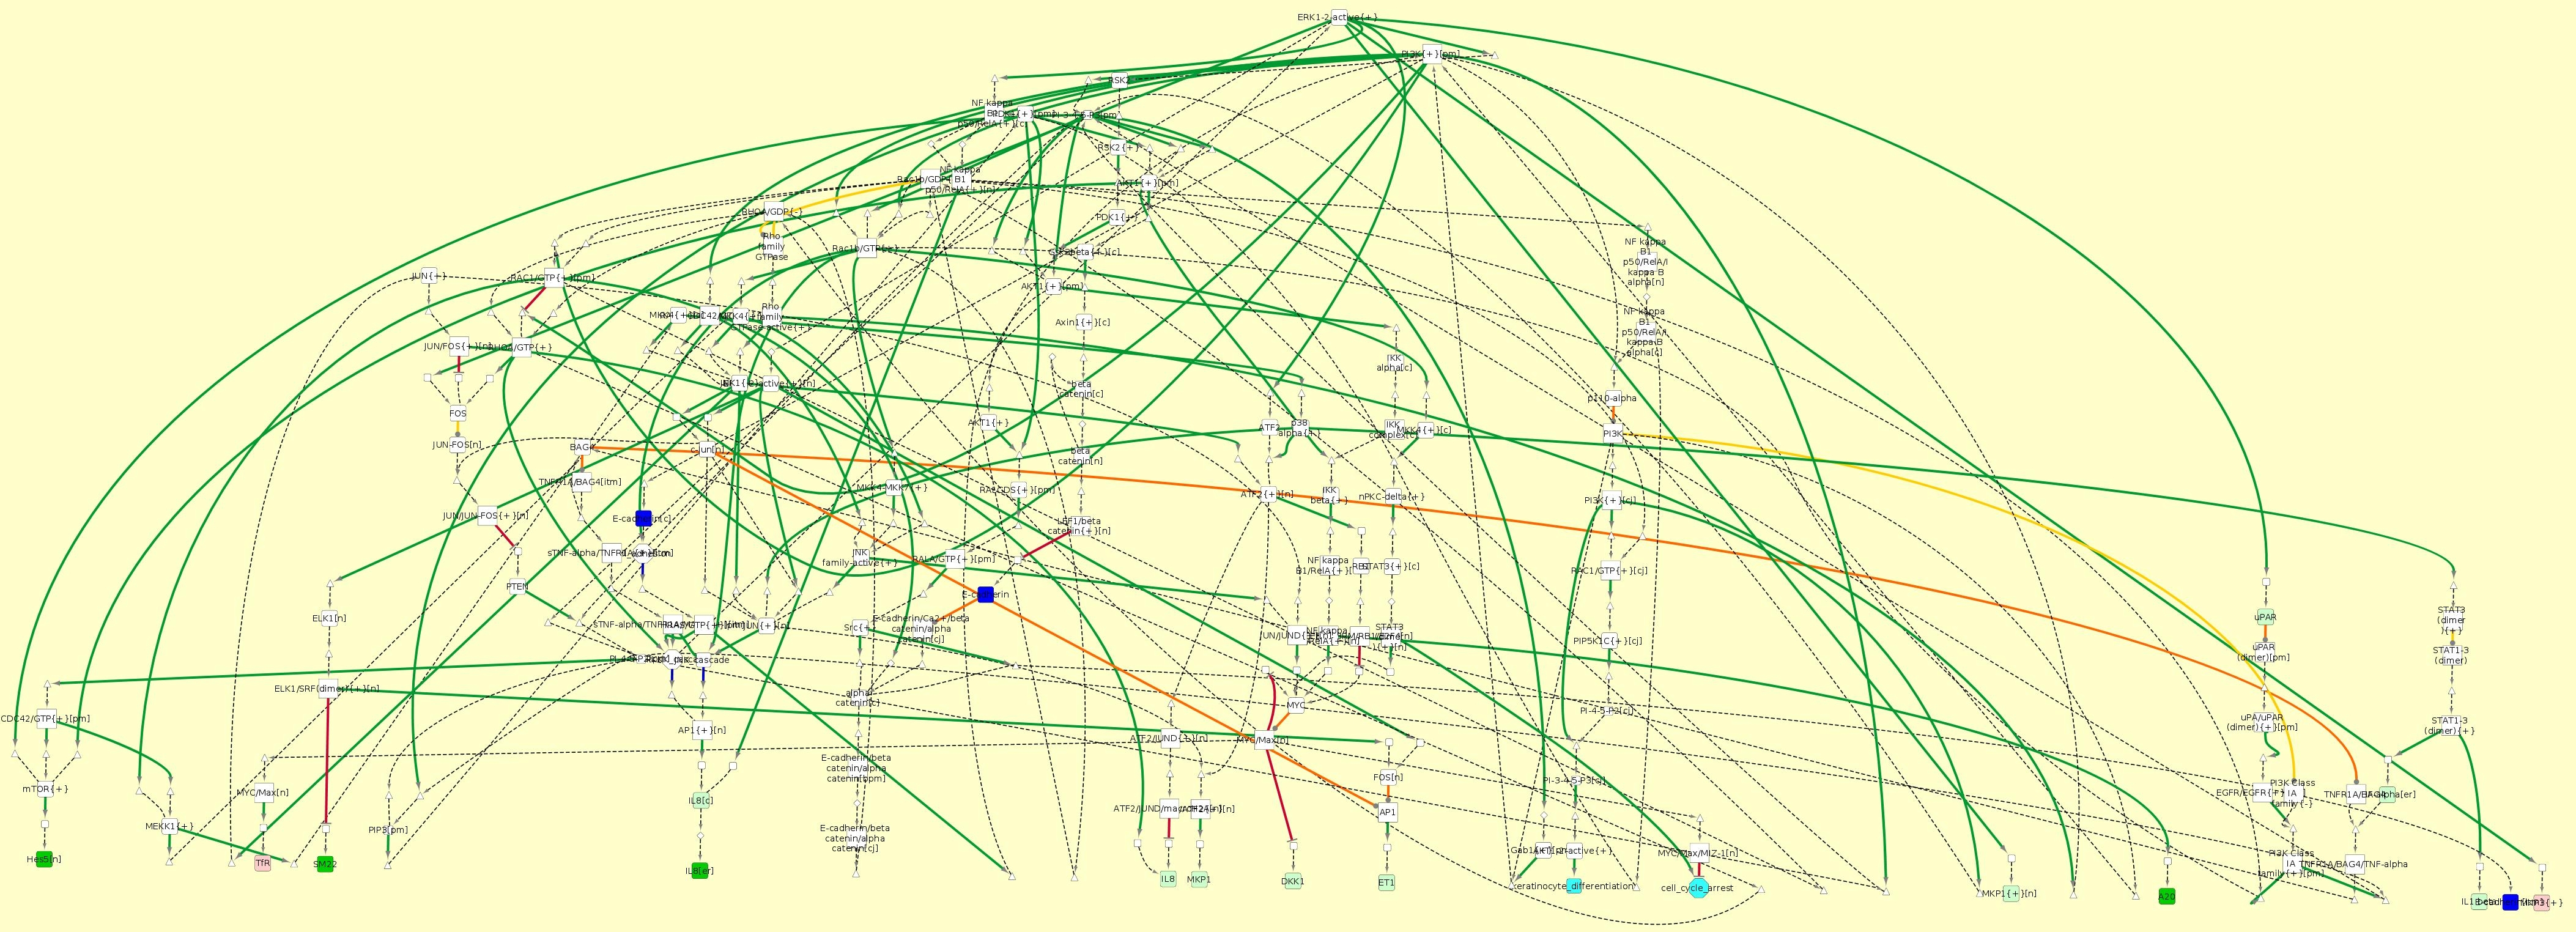
\includegraphics[width=0.45\textwidth]{figs/net.jpg}}
	\zoomIn[left]{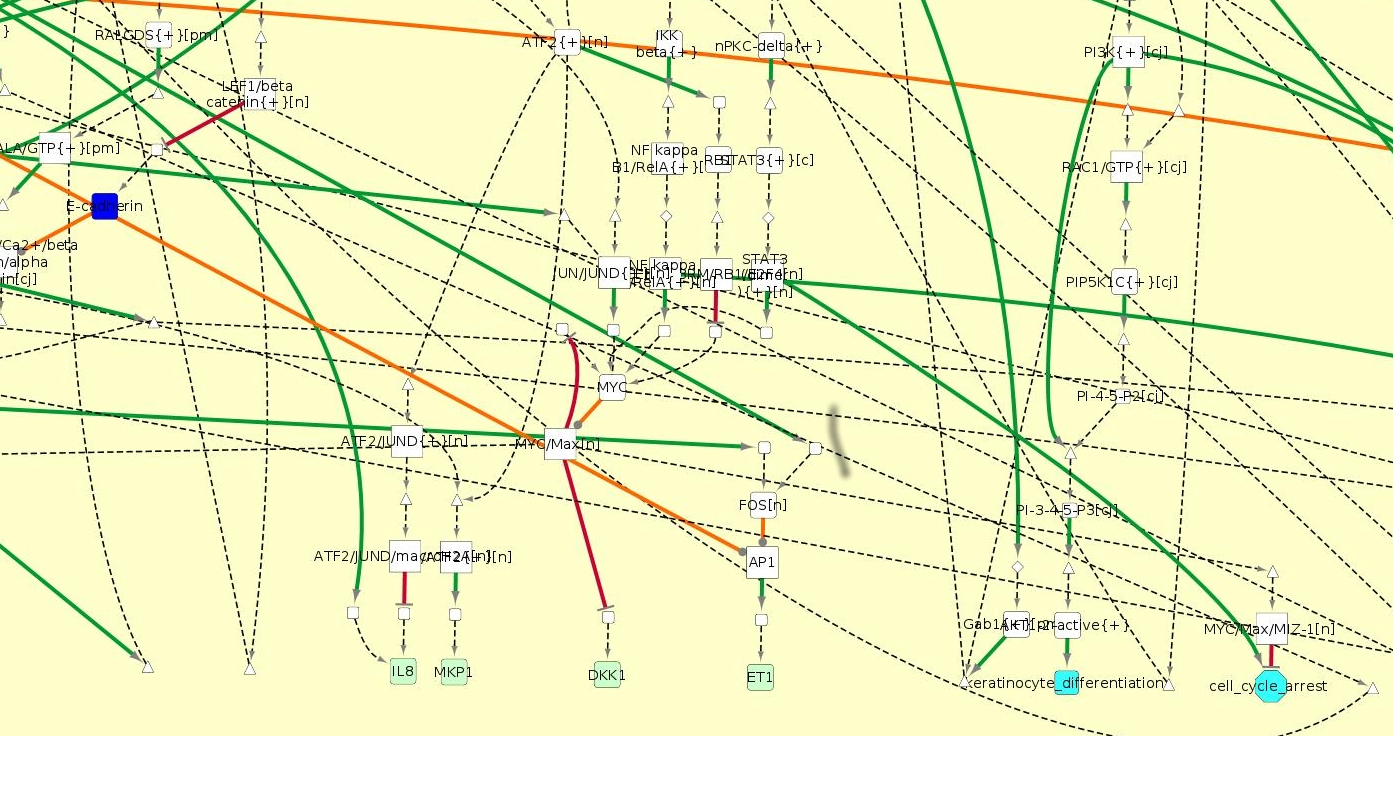
\includegraphics[scale=0.25]{figs/netzoom.png}}{0.35,0.005}{0.320,0.420}
	%\zoomIn{\includegraphics[width=0.45\textwidth]{Geant3}}{0.45,0.475}{0.120,0.120}
	%\zoomIn[left]{\includegraphics[width=0.45\textwidth]{Geant2}}{0.45,0.475}{0.120,0.120}
	%\zoomIn{\includegraphics[width=0.45\textwidth]{Geant1}}{0.45,0.475}{0.120,0.120}
	%\zoomIn[right]{\includegraphics[width=0.45\textwidth]{Geant0}}{0.45,0.475}{0.120,0.120}
\end{tikzpicture}


\end{frame}

%\subsection{Automata Network}
%% Définition du Process Hitting + sortes coopératives

%mettre un RRB ----> en AAN  ----> STate graph 
%rajouter une slide
\begin{frame}
\frametitle{Biological networks modelling}
\begin{tikzpicture}
 \node[scale=1] (brn) at (0,5) {\begin{tikzpicture}[auto,scale=0.9] 
                                                  \path[use as bounding box] (-0.7,-0.3) rectangle (2.5,2);
 
                                                               \node[qgre,scale=0.8] (a) at (0,2) {a};
                                                                \node[mod,scale=0.8] (i) at (1,1) {i};
                                                                \node[qgre,scale=0.8] (b) at (0,0) {b};
                                                                \node[qgre,scale=0.8] (c) at (2,1) {c};
                                                                \path
                                                                  (a) edge[act,scale=0.1] (i)
                                                                  (b) edge[inh,scale=0.1] (i)
                                                                  (i) edge[st,scale=0.1]  (c)
                                                                  ;
                                                               
                                                  \end{tikzpicture}};
%\node (brn) at (0,5) {};
\node[scale=0.6] (an) at (7,5) {\begin{tikzpicture}
\exandef
\end{tikzpicture}};
\node[scale=0.6] (sg) at (2,1) {
\begin{tikzpicture}[line join=bevel,font=\LARGE]
%%
  \node (6) at (405.0bp,18.0bp) [reach,nd4] {$\langle a_2,b_1,c_0\rangle$};
  \node (2) at (405.0bp,90.0bp) [reach,nd3] {$\langle a_2,b_0,c_0\rangle$};
  \node (1) at (570.0bp,90.0bp) [reach,nd1] {$\langle a_1,b_0,c_0\rangle$};
  \node (0) at (469.0bp,162.0bp) [reach,nd0] {$s_0 = \langle a_0,b_0,c_0\rangle$};
  \node (4) at (469.0bp,234.0bp) [reach,nd5] {$\langle a_0,b_1,c_0\rangle$};
 
 
  \draw [->,arc3] (0) ..controls (445.65bp,135.46bp) and (435.95bp,124.86bp)  .. (2);
  \draw [->,arc5] (0) ..controls (475.71bp,188.03bp) and (475.94bp,197.36bp)  .. (4);
  \draw [->,arc4] (2) ..controls (405.0bp,63.983bp) and (405.0bp,54.712bp)  .. (6);
  \draw [->,arc1] (0) ..controls (499.93bp,134.79bp) and (517.41bp,122.58bp)  .. (1);
  \draw [->,arc2] (1) ..controls (539.0bp,117.26bp) and (521.52bp,129.47bp)  .. (0);
  \draw [->,arc5] (4) ..controls (462.3bp,208.35bp) and (462.06bp,199.03bp)  .. (0);
 
%
\end{tikzpicture}

};
\path 
(brn) edge[->,line width=8pt, color=lightgray] (an)
(an) edge[->,line width=8pt, color=lightgray,bend left] (sg)
;
\end{tikzpicture}
\end{frame}


\begin{frame}
  \frametitle{Automata Networks}
  %\framesubtitle{\tcite{Paulev\'e et al. 2012}}


\begin{columns}
\begin{column}{0.6\textwidth}
% 1 : Sortes
\only<1>{
\tikzstyle{process}=[circle,minimum size=15pt,font=\footnotesize,inner sep=1pt]
\tikzstyle{tick label}=[color=white, font=\footnotesize]
\tikzstyle{tick}=[transparent]
\tikzstyle{hit}=[transparent]
\tikzstyle{selfhit}=[transparent, min distance=30pt,curve to]
\tikzstyle{bounce}=[transparent]
\tikzstyle{hlhit}=[transparent]
\tikzstyle{local transitions}=[transparent]
\begin{center}\scalebox{\scaleex}{
\begin{tikzpicture}
\exandef
\end{tikzpicture}
}\end{center}
}

% 2 : Processus
\only<2>{
\tikzstyle{process}=[circle,draw,minimum size=15pt,font=\footnotesize,inner sep=1pt]
\tikzstyle{tick label}=[font=\footnotesize]
\tikzstyle{tick}=[densely dotted]
\tikzstyle{hit}=[transparent]
\tikzstyle{selfhit}=[transparent, min distance=30pt,curve to]
\tikzstyle{bounce}=[transparent]
\tikzstyle{hlhit}=[transparent]
\tikzstyle{local transitions}=[transparent]
\begin{center}\scalebox{\scaleex}{
\begin{tikzpicture}
\exandef
\end{tikzpicture}
}\end{center}
}

% 3 : États
\only<3>{
\tikzstyle{hit}=[transparent]
\tikzstyle{selfhit}=[transparent, min distance=30pt,curve to]
\tikzstyle{bounce}=[transparent]
\tikzstyle{hlhit}=[transparent]
\tikzstyle{local transitions}=[transparent]
\begin{center}\scalebox{\scaleex}{
\begin{tikzpicture}
\exandef

\TState{3}{a_0,b_0,c_0}
\end{tikzpicture}
}\end{center}
}

% 4 : Actions
\only<4->{
\tikzstyle{tick}=[densely dotted]
\tikzstyle{hit}=[->,>=angle 45]
\tikzstyle{selfhit}=[min distance=30pt,curve to]
\tikzstyle{bounce}=[densely dotted,>=stealth',->]
\tikzstyle{hlhit}=[very thick]
\begin{center}\scalebox{\scaleex}{
\begin{tikzpicture}
\exandef
\TState{4}{a_0,b_0,c_0}
\TState{5}{a_1,b_0,c_0}
\TState{6}{a_0,b_0,c_0}
\TState{7}{a_2,b_0,c_0}
\TState{8}{a_2,b_1,c_0}
\end{tikzpicture}
}\end{center}
}
\end{column}

\begin{column}{0.4\textwidth}
\begin{figure}[p]
\centering

\scalebox{0.4}{
\only<4>{
\tikzstyle{arc0}=[transparent]
\tikzstyle{nd0}=[]
\tikzstyle{arc1}=[transparent]
\tikzstyle{nd1}=[transparent]
\tikzstyle{arc2}=[transparent]
\tikzstyle{nd2}=[transparent]
\tikzstyle{arc3}=[transparent]
\tikzstyle{nd3}=[transparent]
\tikzstyle{arc4}=[transparent]
\tikzstyle{nd4}=[transparent]
\tikzstyle{arc5}=[transparent]
\tikzstyle{nd5}=[transparent]

\begin{tikzpicture}[line join=bevel,font=\LARGE]
%%
  \node (6) at (405.0bp,18.0bp) [reach,nd4] {$\langle a_2,b_1,c_0\rangle$};
  \node (2) at (405.0bp,90.0bp) [reach,nd3] {$\langle a_2,b_0,c_0\rangle$};
  \node (1) at (570.0bp,90.0bp) [reach,nd1] {$\langle a_1,b_0,c_0\rangle$};
  \node (0) at (469.0bp,162.0bp) [reach,nd0] {$s_0 = \langle a_0,b_0,c_0\rangle$};
  \node (4) at (469.0bp,234.0bp) [reach,nd5] {$\langle a_0,b_1,c_0\rangle$};
 
 
  \draw [->,arc3] (0) ..controls (445.65bp,135.46bp) and (435.95bp,124.86bp)  .. (2);
  \draw [->,arc5] (0) ..controls (475.71bp,188.03bp) and (475.94bp,197.36bp)  .. (4);
  \draw [->,arc4] (2) ..controls (405.0bp,63.983bp) and (405.0bp,54.712bp)  .. (6);
  \draw [->,arc1] (0) ..controls (499.93bp,134.79bp) and (517.41bp,122.58bp)  .. (1);
  \draw [->,arc2] (1) ..controls (539.0bp,117.26bp) and (521.52bp,129.47bp)  .. (0);
  \draw [->,arc5] (4) ..controls (462.3bp,208.35bp) and (462.06bp,199.03bp)  .. (0);
 
%
\end{tikzpicture}


}
\only<5>{
\tikzstyle{arc0}=[->]
\tikzstyle{nd0}=[]
\tikzstyle{arc1}=[->]
\tikzstyle{nd1}=[]
\tikzstyle{arc2}=[transparent]
\tikzstyle{nd2}=[transparent]
\tikzstyle{arc3}=[transparent]
\tikzstyle{nd3}=[transparent]
\tikzstyle{arc4}=[transparent]
\tikzstyle{nd4}=[transparent]
\tikzstyle{arc5}=[transparent]
\tikzstyle{nd5}=[transparent]

\begin{tikzpicture}[line join=bevel,font=\LARGE]
%%
  \node (6) at (405.0bp,18.0bp) [reach,nd4] {$\langle a_2,b_1,c_0\rangle$};
  \node (2) at (405.0bp,90.0bp) [reach,nd3] {$\langle a_2,b_0,c_0\rangle$};
  \node (1) at (570.0bp,90.0bp) [reach,nd1] {$\langle a_1,b_0,c_0\rangle$};
  \node (0) at (469.0bp,162.0bp) [reach,nd0] {$s_0 = \langle a_0,b_0,c_0\rangle$};
  \node (4) at (469.0bp,234.0bp) [reach,nd5] {$\langle a_0,b_1,c_0\rangle$};
 
 
  \draw [->,arc3] (0) ..controls (445.65bp,135.46bp) and (435.95bp,124.86bp)  .. (2);
  \draw [->,arc5] (0) ..controls (475.71bp,188.03bp) and (475.94bp,197.36bp)  .. (4);
  \draw [->,arc4] (2) ..controls (405.0bp,63.983bp) and (405.0bp,54.712bp)  .. (6);
  \draw [->,arc1] (0) ..controls (499.93bp,134.79bp) and (517.41bp,122.58bp)  .. (1);
  \draw [->,arc2] (1) ..controls (539.0bp,117.26bp) and (521.52bp,129.47bp)  .. (0);
  \draw [->,arc5] (4) ..controls (462.3bp,208.35bp) and (462.06bp,199.03bp)  .. (0);
 
%
\end{tikzpicture}


}
\only<6>{
\tikzstyle{arc0}=[->]
\tikzstyle{nd0}=[]
\tikzstyle{arc1}=[->]
\tikzstyle{nd1}=[]
\tikzstyle{arc2}=[->]
\tikzstyle{nd2}=[]
\tikzstyle{arc3}=[transparent]
\tikzstyle{nd3}=[transparent]
\tikzstyle{arc4}=[transparent]
\tikzstyle{nd4}=[transparent]
\tikzstyle{arc5}=[transparent]
\tikzstyle{nd5}=[transparent]

\begin{tikzpicture}[line join=bevel,font=\LARGE]
%%
  \node (6) at (405.0bp,18.0bp) [reach,nd4] {$\langle a_2,b_1,c_0\rangle$};
  \node (2) at (405.0bp,90.0bp) [reach,nd3] {$\langle a_2,b_0,c_0\rangle$};
  \node (1) at (570.0bp,90.0bp) [reach,nd1] {$\langle a_1,b_0,c_0\rangle$};
  \node (0) at (469.0bp,162.0bp) [reach,nd0] {$s_0 = \langle a_0,b_0,c_0\rangle$};
  \node (4) at (469.0bp,234.0bp) [reach,nd5] {$\langle a_0,b_1,c_0\rangle$};
 
 
  \draw [->,arc3] (0) ..controls (445.65bp,135.46bp) and (435.95bp,124.86bp)  .. (2);
  \draw [->,arc5] (0) ..controls (475.71bp,188.03bp) and (475.94bp,197.36bp)  .. (4);
  \draw [->,arc4] (2) ..controls (405.0bp,63.983bp) and (405.0bp,54.712bp)  .. (6);
  \draw [->,arc1] (0) ..controls (499.93bp,134.79bp) and (517.41bp,122.58bp)  .. (1);
  \draw [->,arc2] (1) ..controls (539.0bp,117.26bp) and (521.52bp,129.47bp)  .. (0);
  \draw [->,arc5] (4) ..controls (462.3bp,208.35bp) and (462.06bp,199.03bp)  .. (0);
 
%
\end{tikzpicture}


}
\only<7>{
\tikzstyle{arc0}=[->]
\tikzstyle{nd0}=[]
\tikzstyle{arc1}=[->]
\tikzstyle{nd1}=[]
\tikzstyle{arc2}=[->]
\tikzstyle{nd2}=[]
\tikzstyle{arc3}=[->]
\tikzstyle{nd3}=[]
\tikzstyle{arc4}=[transparent]
\tikzstyle{nd4}=[transparent]
\tikzstyle{arc5}=[transparent]
\tikzstyle{nd5}=[transparent]

\begin{tikzpicture}[line join=bevel,font=\LARGE]
%%
  \node (6) at (405.0bp,18.0bp) [reach,nd4] {$\langle a_2,b_1,c_0\rangle$};
  \node (2) at (405.0bp,90.0bp) [reach,nd3] {$\langle a_2,b_0,c_0\rangle$};
  \node (1) at (570.0bp,90.0bp) [reach,nd1] {$\langle a_1,b_0,c_0\rangle$};
  \node (0) at (469.0bp,162.0bp) [reach,nd0] {$s_0 = \langle a_0,b_0,c_0\rangle$};
  \node (4) at (469.0bp,234.0bp) [reach,nd5] {$\langle a_0,b_1,c_0\rangle$};
 
 
  \draw [->,arc3] (0) ..controls (445.65bp,135.46bp) and (435.95bp,124.86bp)  .. (2);
  \draw [->,arc5] (0) ..controls (475.71bp,188.03bp) and (475.94bp,197.36bp)  .. (4);
  \draw [->,arc4] (2) ..controls (405.0bp,63.983bp) and (405.0bp,54.712bp)  .. (6);
  \draw [->,arc1] (0) ..controls (499.93bp,134.79bp) and (517.41bp,122.58bp)  .. (1);
  \draw [->,arc2] (1) ..controls (539.0bp,117.26bp) and (521.52bp,129.47bp)  .. (0);
  \draw [->,arc5] (4) ..controls (462.3bp,208.35bp) and (462.06bp,199.03bp)  .. (0);
 
%
\end{tikzpicture}


}
\only<8>{
\tikzstyle{arc0}=[->]
\tikzstyle{nd0}=[]
\tikzstyle{arc1}=[->]
\tikzstyle{nd1}=[]
\tikzstyle{arc2}=[->]
\tikzstyle{nd2}=[]
\tikzstyle{arc3}=[->]
\tikzstyle{nd3}=[]
\tikzstyle{arc4}=[->]
\tikzstyle{nd4}=[]
\tikzstyle{arc5}=[transparent]
\tikzstyle{nd5}=[transparent]

\begin{tikzpicture}[line join=bevel,font=\LARGE]
%%
  \node (6) at (405.0bp,18.0bp) [reach,nd4] {$\langle a_2,b_1,c_0\rangle$};
  \node (2) at (405.0bp,90.0bp) [reach,nd3] {$\langle a_2,b_0,c_0\rangle$};
  \node (1) at (570.0bp,90.0bp) [reach,nd1] {$\langle a_1,b_0,c_0\rangle$};
  \node (0) at (469.0bp,162.0bp) [reach,nd0] {$s_0 = \langle a_0,b_0,c_0\rangle$};
  \node (4) at (469.0bp,234.0bp) [reach,nd5] {$\langle a_0,b_1,c_0\rangle$};
 
 
  \draw [->,arc3] (0) ..controls (445.65bp,135.46bp) and (435.95bp,124.86bp)  .. (2);
  \draw [->,arc5] (0) ..controls (475.71bp,188.03bp) and (475.94bp,197.36bp)  .. (4);
  \draw [->,arc4] (2) ..controls (405.0bp,63.983bp) and (405.0bp,54.712bp)  .. (6);
  \draw [->,arc1] (0) ..controls (499.93bp,134.79bp) and (517.41bp,122.58bp)  .. (1);
  \draw [->,arc2] (1) ..controls (539.0bp,117.26bp) and (521.52bp,129.47bp)  .. (0);
  \draw [->,arc5] (4) ..controls (462.3bp,208.35bp) and (462.06bp,199.03bp)  .. (0);
 
%
\end{tikzpicture}


}
\only<9>{
\tikzstyle{arc0}=[->]
\tikzstyle{nd0}=[]
\tikzstyle{arc1}=[->]
\tikzstyle{nd1}=[]
\tikzstyle{arc2}=[->]
\tikzstyle{nd2}=[]
\tikzstyle{arc3}=[->]
\tikzstyle{nd3}=[]
\tikzstyle{arc4}=[->]
\tikzstyle{nd4}=[]
\tikzstyle{arc5}=[->]
\tikzstyle{nd5}=[]

\begin{tikzpicture}[line join=bevel,font=\LARGE]
%%
  \node (6) at (405.0bp,18.0bp) [reach,nd4] {$\langle a_2,b_1,c_0\rangle$};
  \node (2) at (405.0bp,90.0bp) [reach,nd3] {$\langle a_2,b_0,c_0\rangle$};
  \node (1) at (570.0bp,90.0bp) [reach,nd1] {$\langle a_1,b_0,c_0\rangle$};
  \node (0) at (469.0bp,162.0bp) [reach,nd0] {$s_0 = \langle a_0,b_0,c_0\rangle$};
  \node (4) at (469.0bp,234.0bp) [reach,nd5] {$\langle a_0,b_1,c_0\rangle$};
 
 
  \draw [->,arc3] (0) ..controls (445.65bp,135.46bp) and (435.95bp,124.86bp)  .. (2);
  \draw [->,arc5] (0) ..controls (475.71bp,188.03bp) and (475.94bp,197.36bp)  .. (4);
  \draw [->,arc4] (2) ..controls (405.0bp,63.983bp) and (405.0bp,54.712bp)  .. (6);
  \draw [->,arc1] (0) ..controls (499.93bp,134.79bp) and (517.41bp,122.58bp)  .. (1);
  \draw [->,arc2] (1) ..controls (539.0bp,117.26bp) and (521.52bp,129.47bp)  .. (0);
  \draw [->,arc5] (4) ..controls (462.3bp,208.35bp) and (462.06bp,199.03bp)  .. (0);
 
%
\end{tikzpicture}


}
}

\end{figure}

\end{column}
\end{columns}
%\medskip

\begin{liste}
  \item \tval{Automata}: components \qex{$a$, $b$, $c$}
\pause[2]
  \item \tval{local states}: levels of expression \qex{$c_0$, $c_1$, $c_2$}
\pause[3]
  \item \tval{States}: sets of active local states%
  \only<3-4>{\qex{$\PHetat{a_0, b_0, c_0}$}}%
  \only<5>{\qex{$\PHetat{a_1, b_0, c_0}$}}%
  \only<6>{\qex{$\PHetat{a_0, b_0, c_0}$}}%
  \only<7>{\qex{$\PHetat{a_2, b_0, c_0}$}}%
  \only<8>{\qex{$\PHetat{a_2, b_1, c_0}$}}
\pause[4]
  \item \tval{Transitions}: dynamics \qex{\only<5>{\underline}{$t_1 = \trans{a_0}{a_1}{b_0}$}, \only<6>{\underline}{$t_2 = \trans{a_1}{a_0}{}$}, \only<7>{\underline}{$t_3 = \trans{a_0}{a_2}{b_0,c_0}$}, \only<8>{\underline}{$t_4 = \trans{b_0}{b_1}{}$}}
\end{liste}
%une seule transition à la fois
%on peut avoir un choix il faut bien expliquer ça.
\end{frame}


%% Stochasticité

\begin{frame}
  \frametitle{Stochastic Features}
  \framesubtitle{\tcite{Paulev\'e et al. 2010}}

\begin{itemize}
  \item Introduces time features
  \item Parameters: either $(r,sa)$, or the \tval{firing interval} $[d;D]$.
  \begin{fleches}
    \item Tests by simulation
  \end{fleches}
\end{itemize}

%\begin{columns}
%\begin{column}{0.5\textwidth}

\only<1->{
\scalebox{0.9}{
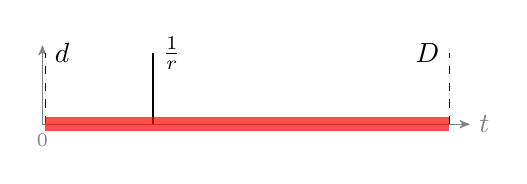
\begin{tikzpicture}[plot,xscale=0.35,yscale=1]
\draw[axe] (0,0) -- (15.5,0) node[right] {$t$};
\draw[axe] (0,0) -- (0,1);
\draw[ticks] (0,0) node[below] {$0$};
\draw[mean] (4,0) -- (4,0.9) node[right]{$\frac{1}{r}$};
\draw[dashed] (0.10127,0) -- (0.10127,0.9) node[right] {$d$} (14.75552,0) --
(14.75552,0.9) node[left] {$D$};
\pgfplothandlerlineto
\pgfplotxyfile{plots/BioAtlanSTIC-0409/erlang-0.25-1.table}
\pgfusepath{stroke}
\draw[interval] (0.10127,0) -- (14.75552,0);
\end{tikzpicture}
}

\scalebox{0.9}{
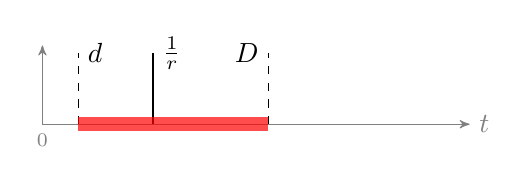
\begin{tikzpicture}[plot,xscale=0.35,yscale=1]
\draw[axe] (0,0) -- (15.5,0) node[right] {$t$};
\draw[axe] (0,0) -- (0,1);
\draw[ticks] (0,0) node[below] {$0$};
\draw[mean] (4,0) -- (4,0.9) node[right]{$\frac{1}{r}$};
\draw[dashed] (1.29879,0) -- (1.29879,0.9) node[right] {$d$} (8.19327,0) --
(8.19327,0.9) node[left] {$D$};
\pgfplothandlerlineto
\pgfplotxyfile{plots/BioAtlanSTIC-0409/erlang-0.25-5.table}
\pgfusepath{stroke}
\draw[interval] (1.29879,0) -- (8.19327,0);
\end{tikzpicture}
}

\scalebox{0.9}{
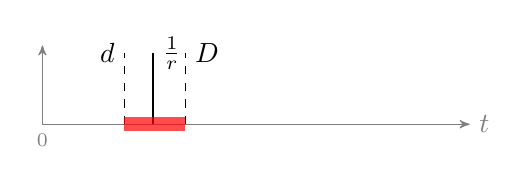
\begin{tikzpicture}[plot,xscale=0.35,yscale=1]
\draw[axe] (0,0) -- (15.5,0) node[right] {$t$};
\draw[axe] (0,0) -- (0,1);
\draw[ticks] (0,0) node[below] {$0$};
\draw[mean] (4,0) -- (4,0.9) node[right]{$\frac{1}{r}$};
\draw[dashed] (2.96888,0) -- (2.96888,0.9) node[left] {$d$} (5.18245,0) --
(5.18245,0.9) node[right] {$D$};
\pgfplothandlerlineto
\pgfplotxyfile{plots/BioAtlanSTIC-0409/erlang-0.25-50.table}
\pgfusepath{stroke}
\draw[interval] (2.96888,0) -- (5.18245,0);
\end{tikzpicture}
}

~~\textcolor{lightred}{\rule{17mm}{4.5pt}} ~ action duration
}

%\end{column}
\end{frame}

%%%explain the automatic model construction

\begin{frame}[c]
\frametitle{Network topology}
\framesubtitle{Automatic patterns detection and transformation}

%We have two procedures that allow us to detect and translate RSTC network to the Process Hitting model.

\begin{tikzpicture}[auto]
 
 % placement des noeuds
 
 %\node[cloud, cloud puffs = 10, draw, minimum width = 0.1cm, minimum height = 0.1cm, fill = gray!10, scale=0.3] (rstcbis) at (-2,13){
 %  \begin{tabular}{c}
 %  \textbf{Biological network} \\ \hline
 %  RSTC network
 % \end{tabular}};
 
 \node (rep) at (0,-5) {};
  
  \node[es,align=center,scale=0.5] (rstcbis) at (-2,11.5) {\begin{tabular}{c}
                                            \textbf{Biological network} \\ \hline
                                            RSTC network
                                           \end{tabular}};

 
\onslide<2->{
%\draw[-open triangle 90] (0,12.5) -- (0.2,12.5);
 \node[instruct,align=center, scale=0.7] (pro1) at (0.5,11.5) {\begin{tabular}{c}
                                            \textbf{Patterns Detection} \\ \hline
                                            in  RSTC network
                                          \end{tabular}};
      
 \path
  (rstcbis) edge[st] (pro1);
}
                                          
 \onslide<3->{
 %\draw[-open triangle 90] (2,12.5) -- (2.5,12.5);
 \node[es, scale=0.5] (sop) at (3,11.5) {\begin{tabular}{c}
                                            \textbf{Set of patterns} \\ \hline
                                            of RSTC network
                                           \end{tabular}};

\path
   (pro1) edge[st] (sop);
                                           
\node[scale=0.8] (bpat) at (-1,8) {\begin{tabular}{|c|}
\hline
\textbf{Biological Patterns}

\\ \hline
\begin{tikzpicture}
\node[scale=0.7] (sa1) at (0,0){\begin{tikzpicture}[auto]
\path[use as bounding box] (-0.7,-0.3) rectangle (2.5,2);

\node[qgre] (a) at (0,0.5) {a};
\node[mod] (i) at (1,0.5) {i};
\node[qgre] (b) at (2,0.5) {b};
\node[es] (d) at (1,1.5) {Simple activation};

% a restorer
\path
 (a) edge[act] (i)
 (i) edge[st]  (b);
\end{tikzpicture}};
\end{tikzpicture}

\\ \hline

\begin{tikzpicture}
\node[scale=0.7] (si1) at (0,0){\begin{tikzpicture}[auto]
\path[use as bounding box] (-0.7,-0.3) rectangle (2.5,2);

\node[qgre] (a) at (0,0.5) {a};
\node[mod] (i) at (1,0.5) {i};
\node[qgre] (b) at (2,0.5) {b};
\node[es] (d) at (1,1.5) {Simple inhibition};

%a restorer 
\path
 (a) edge[inh] (i)
 (i) edge[st]  (b);
 \end{tikzpicture}};
\end{tikzpicture}


\\ \hline

\begin{tikzpicture}
\node[scale=0.7] (sai1) at (0,0){\begin{tikzpicture}[auto]
\path[use as bounding box] (-0.7,-0.3) rectangle (2.5,3);
\node[qgre] (a) at (0,2) {a};
\node[mod] (i) at (1,1) {i};
\node[qgre] (b) at (0,0) {b};
\node[qgre] (c) at (2,1) {c};
\node[es] (d) at (1,3) {activation or inhibition};

% arestorer
\path
 (a) edge[act] (i)
 (b) edge[inh] (i)
 (i) edge[st]  (c);
\end{tikzpicture}};
\end{tikzpicture}

\\ \hline

\end{tabular}
};

}


\onslide<4->{

\node[es,scale=0.5] (timed) at (3,10.5) {\begin{tabular}{c}
                                            \textbf{Time delay} \\ \hline
                                            Estimate from TSD
                                           \end{tabular}};


 \node[instruct,align=center, scale=0.7] (pro2) at (5.5,11.5) {\begin{tabular}{c}
                                            \textbf{Patterns translation} \\ \hline
                                            in  AN (PH) model
                                           \end{tabular}};
 \path
    (sop) edge[st] (pro2)
    (timed) edge[st] (pro2);
 }
 
 \onslide<5->{
   
   \node[es,scale=0.5] (php) at (8,11.5) {\begin{tabular}{c}
                                            \textbf{AN (PH) Patterns} \\
                                           \end{tabular}};
\path
   (pro2) edge[st] (php);

\node[scale=0.8] (phpat) at (6.8,8) {\begin{tabular}{|c|c|}
\hline

\textbf{AN (Process Hitting) Transformations}

 \\ \hline

\begin{tikzpicture}
%\exphpatact
\node[scale=0.5] (sa) at (0,0) {\begin{tikzpicture}
\exphpatact
\end{tikzpicture}};
\end{tikzpicture}


\\ \hline


\begin{tikzpicture}
%\exphpatact
\node[scale=0.5] (sa) at (0,0) {\begin{tikzpicture}
\exphpatini
\end{tikzpicture}};
\end{tikzpicture}

 \\ \hline


\begin{tikzpicture}
%\exphpatact
\node[scale=0.5] (sai) at (0,0) {\begin{tikzpicture}
\exphpatai
\end{tikzpicture}};
\end{tikzpicture}
\\ \hline

\end{tabular}
};
}
\end{tikzpicture}

%exemple of patterns 


\end{frame}


\begin{frame}[c]
 \frametitle{Network topology}
 \framesubtitle{Automatic patterns detection (method)} 

\begin{columns}
\begin{column}{0.6\textwidth}

\begin{tikzpicture}[auto]

\node[qgre] (a1) at (-3,-3) {a};
\node[qgre] (a2) at (-1,-3) {b};
\node[qgre] (a3) at (1,-3) {c};
\node[qgre] (a4) at (3,-3) {d};
%\node[qgre] (a5) at (5,-3) {e};

\node[mod] (i1) at (-3,-2) {};
\node[mod] (i2) at (-1,-2) {};
\node[mod] (i3) at (1,-2) {};
\node[mod] (i4) at (3,-2) {};
%\node[mod] (i5) at (5,-2) {};

\node[ps] (ps1) at (-3,-1) {PS1};
\node[ps] (ps2) at (-1,-1) {PS2};
\node[ps] (ps3) at (1,-1) {PS3};
\node[ps] (ps4) at (3,-1) {PS4};
%\node[ps] (ps5) at (5,-1) {PS5};

\node[mod] (i6) at (-3,0) {};
%\node[mod] (i7) at (-1,0) {};
\node[mod] (i8) at (1,0) {};
\node[mod] (i9) at (3,0) {};
%\node[mod] (i10) at (5,0) {};

\node[ps] (ps6) at (-3,1) {PS6};
%\node[ps] (ps7) at (-1,1) {PS7};
\node[ps] (ps8) at (1,1) {PS8};
\node[ps] (ps9) at (3,1) {PS9};
%\node[ps] (ps10) at (5,1) {PS10};

%les complex
\node[ecad] (d) at (0,3) {Ecad};
\node[cplx] (c1) at (2,-1) {cplx1};
\node[cplx] (c2) at (0,1) {cplx2};
\node[cplx] (c3) at (-2,-1) {cplx3};
\node[cplx] (c4) at (-2,1) {cplx4};
\node[cplx] (c5) at (0,0) {cplx5};
\node[cplx] (c6) at (2,1) {cplx6};

%les seed node
\node[sn] (sn1) at (-2,-3) {SN1};
\node[sn] (sn2) at (2,-3) {SN2};


%les edges 

\path
 (i1) edge[st] (a1)
 (i2) edge[st] (a2)
 (i3) edge[st]  (a3)
 (i4) edge[st]  (a4)
 %(i5) edge[st]  (a5)
 
 (ps1) edge[act] (i1)
 (ps2) edge[act] (i2)
 (ps3) edge[act] (i2)
 (ps3) edge[act] (i3)
 (ps4) edge[act] (i4)
 %(ps5) edge[act] (i5)
 
 (i6) edge[st] (ps1)
 (i6) edge[st] (ps2)
 (i8) edge[st] (ps3)
 (i9) edge[st] (ps4)
 (i9) edge[st] (ps4)
 %(i9) edge[st] (ps5)
 %(i10) edge[st] (ps5)
 
 (ps6) edge[act] (i6)
 (ps8) edge[act] (i8)
 (ps9) edge[act] (i9)
 %(ps10) edge[act] (i10)
 
 (d) edge[act] (ps6)
 (d) edge[act] (ps8)
 (d) edge[act] (ps9)
 %(d) edge[act] (ps10)
 
 (c4) edge[act] (c5)
 (c2) edge[act] (c5)
 (d) edge[act] (c2)
 (c5) edge[inh] (ps2)
 (c6) edge[act] (i8)
 (c6) edge[act] (i9)
 (i8) edge[st] (c1)
 (i9) edge[st] (c1)
 (c1) edge[act] (i4)
 
 (ps3) edge[inh] (sn2)
 (i4) edge[st] (sn2)
 
 (ps1) edge[inh] (sn1)
 (c3) edge[act] (sn1)
 (c4) edge[act] (c3)
 
 (a1) edge[inh, bend left] (ps6);
 

 %pattern 1
\only<2-5>{
\node[snpat] (snpat1) at (1,-3) {};
}
\only<3-5>{
\path
 (a3) edge[stv] (i3);
 }
 \only<4-5>{
\path
 (i3) edge[stv] (ps3);
 }
  \only<5>{
\node[snpat] (snpat2) at (1,-1) {};
}

  %le pattern rajouté
\only<5-9>{
\node[scale=0.9] (patraj1) at (5,-2){\begin{tikzpicture}[auto]
\path[use as bounding box] (-0.7,-0.3) rectangle (2.5,2);

\node[ps] (aps3) at (0,0.5) {PS3};
\node[mod] (ips3) at (1,0.5) {i};
\node[qgre] (cps3) at (2,0.5) {c};

% a restorer
\path
 (aps3) edge[act] (ips3)
 (ips3) edge[st]  (cps3);
\end{tikzpicture}};

}

%pattern 2

%le pattern rajouté
\only<9>{
\node[scale=0.9] (sai1) at (5,-3.5){\begin{tikzpicture}[auto]
\path[use as bounding box] (-0.7,-0.3) rectangle (2.5,3);
\node[ps] (aps2) at (0,2) {PS2};
\node[mod] (ips2) at (1,1) {i};
\node[ps] (bps3) at (0,0) {PS3};
\node[qgre] (cb) at (2,1) {b};

% arestorer
\path
 (aps2) edge[act] (ips2)
 (bps3) edge[act] (ips2)
 (ips2) edge[st]  (cb);
\end{tikzpicture}};


}

 \only<6-9>{
\node[snpat] (snpat3) at (-1,-3) {};
}


 \only<7-9>{
\path
 (a2) edge[stv] (i2);
 }
 \only<8-9>{
\path
 (i2) edge[stv] (ps2)
 (i2) edge[stv] (ps3);
 }
 
  \only<9>{
\node[snpat] (snpat4) at (-1,-1) {};
\node[snpat] (snpat5) at (1,-1) {};
}


 
\end{tikzpicture}

\end{column}

\begin{column}{0.4\textwidth}
Two main types of nodes:
 \begin{liste}
  \item \tval{Terminal Nodes:} proteins, complexes, mRNA expressions, cellular states,...
  \item \tval{Transient Nodes:} translocations, modifications, transcriptions,...
 \end{liste}
 
 \only<10->{
 \tval{Complexity}:
 The algorithm  has a time complexity of \tval{$\mathcal{O}(|V|\log{}(h))$}. 
  Where 
  \begin{liste}
  \item \tval{$|V|$} is the set of nodes and \tval{$|E|$} is the set of edges.
  \item $h$ is the average height of the patterns in the RSTC network. In the worst case 
  $h = \log_{|V|}(|V|)$.
 \end{liste}
 }
\end{column}



\end{columns}

\end{frame}


%\subsection{Stochastic Parameters Estimation \& Integration}
%\begin{frame}[c]
  \frametitle{Time series data}
  
\begin{center}
  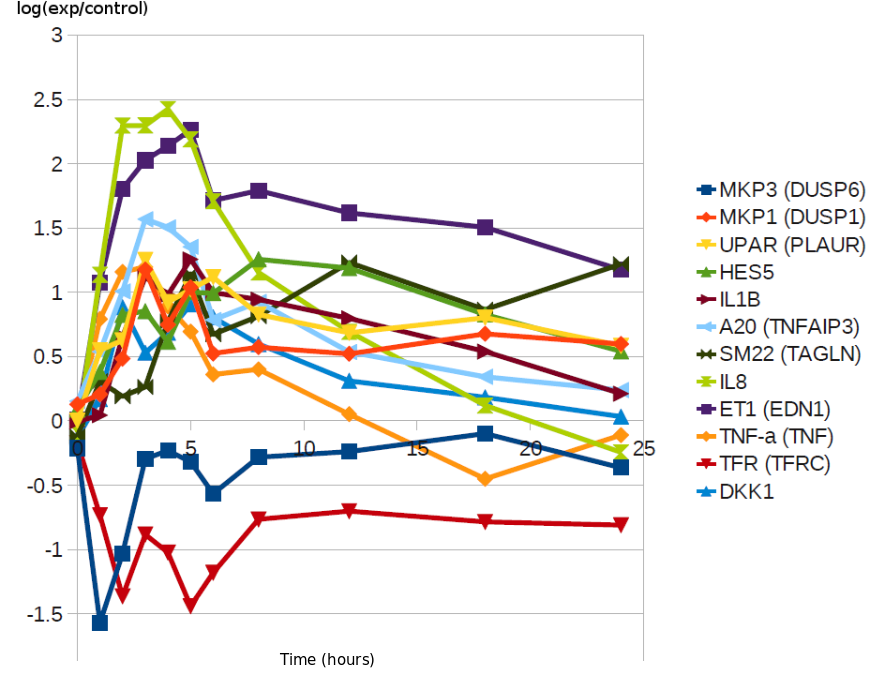
\includegraphics[width=70mm]{figs/12genes.png}
\end{center}

%\pause

\begin{columns}
\begin{column}{0.7\textwidth}
\begin{itemize}
  \item Experiment: \tval{calcium stimuli}
  \item Measured at 10 time-points(0-24hrs)
  \item \tval{$200$ transcripts} selected  (\tval{dynamic patterns}) %their fold expression with respect to the non-stimulated cell was significant in at least one time point
  \item We included in our model a subset of $12$ of them
\end{itemize}
\end{column}

\begin{column}{0.3\textwidth}
% \textbf{ \small Prof. Dr. Peter Angel
%Signal Transduction and Growth Control (A100)
%German Cancer research center
%Heidelberg, Germany}

\end{column}
\end{columns}
%\textcolor{couleurtheme}{$\Rightarrow$} \fbox{\tval{\large Allow efficient translation from Process Hitting to BRN}} \textcolor{couleurtheme}{$\Leftarrow$}

\end{frame}


%
\begin{frame}[c]
 \frametitle{Data integration}
 \framesubtitle{Parameters inference/Principe}
 
\begin{columns}

\begin{column}{0.7\textwidth}
\scalebox{0.9}{
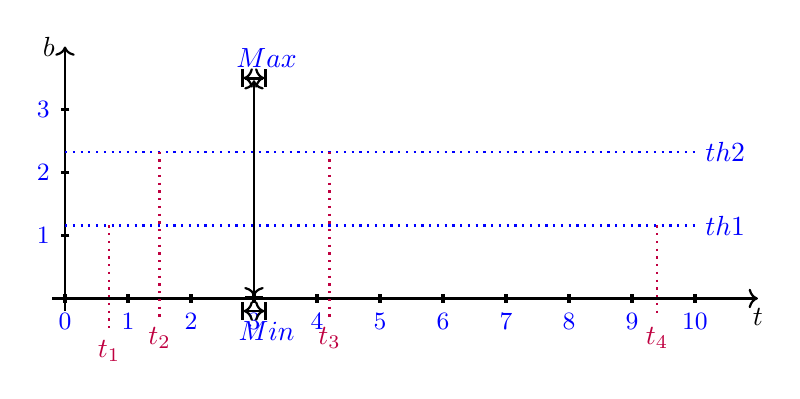
\begin{tikzpicture}[scale = 0.8]
    % Tracé de la parabole
    %\draw[red, domain = -2.2:2.2, smooth] plot (\x, {(\x)^2});
    % Alternative par Gnuplot
    %\draw[red, domain = -2.2:2.2, smooth] plot function{x**2};
    % Lignes tiretées
      \draw[thick, ->] (-.2,0)--(11,0) node[below]{$t$};
     \foreach \t in {0,1,2,3,4,...,10}
      \draw[very thick] (\t,2pt)--(\t,-2pt) node[below,blue]{\small\t};

     \draw[thick, ->] (0,-.2)--(0,4) node[left]{$b$};
     \foreach \y in {1,2,3}
      \draw[very thick] (2pt,\y)--(-2pt,\y) node[left,blue]{\small\y};
      
    \draw[thick] plot[mark=ball,mark size=1pt] file {illustration.txt};
    
    \onslide<2->{
    \draw[thick,|<->|] (2.8,3.5) -- (3.2,3.5) node[above,blue]{$Max$};
    \draw[thick,|<->|] (2.8,-.2) -- (3.2,-.2) node[below,blue]{$Min$};
    }
    \onslide<3->{
    \draw[thick,|<->|] (3,0) -- (3,3.5);
    }
    \onslide<4->{
    \draw[thick,dotted,blue] (0,1.16) -- (10,1.16) node[right]{$th1$}; 
    \draw[thick,dotted,blue] (0,2.33) -- (10,2.33) node[right]{$th2$}; 
    }
    \onslide<5->{
    \draw[thick,dotted,purple] (0.7,1.16) -- (0.7,-.5) node[below]{$t_{1}$};
    }
    \onslide<6->{
    \draw[thick,dotted,purple] (1.5,2.33) -- (1.5,-.3) node[below]{$t_{2}$};
    }
    \onslide<7->{
    \draw[thick,dotted,purple] (4.2,2.33) -- (4.2,-.3) node[below]{$t_{3}$};
    }
    \onslide<8->{
    \draw[thick,dotted,purple] (9.4,1.16) -- (9.4,-.3) node[below]{$t_{4}$};
    }
\end{tikzpicture}
}
%If we assume that $t_{0}=0$,\\
\onslide<5->{$\PHfrappe{a_1}{b_0}{b_1}$ with $r_{1}=\frac{1}{t_{1}-t_{0}}$\\}
\onslide<6->{$\PHfrappe{a_1}{b_1}{b_2}$ with $r_{2}=\frac{1}{t_{2}-t_{1}}$\\}
\onslide<7->{$\PHfrappe{a_0}{b_2}{b_1}$ with $r_{3}=\frac{1}{t_{3}-t_{2}}$\\}
\onslide<8->{$\PHfrappe{a_0}{b_1}{b_0}$ with $r_{4}=\frac{1}{t_{4}-t_{3}}$\\}
\onslide<8->{The formula to estimate the rate of the dynamics of a component according to it TSD is 
\tval{ \Large {$r_{i}=\frac{1}{t_{i}-t_{i-1}}$}}}
\end{column}

\begin{column}{0.3\textwidth}
\scalebox{0.9}{
 \begin{tikzpicture}[scale=0.8]
\path[use as bounding box] (-1,-1) rectangle (2,2);


\TSort{(0,1)}{b}{3}{r}


\only<5->{\TSort{(2,1)}{a}{2}{l}}
\only<5>{
\THit{a_1}{}{b_0}{.east}{b_1}
%\THit{a_0}{out=-120,in=180,selfhit}{a_0}{.west}{a_1}
\path[bounce]
%\TBounce{a_0}{bend left}{a_1}{.south}
\TBounce{b_0}{bend right}{b_1}{.south}
;
\TState{5}{a_1,b_0}
\TState{5}{a_1,b_1}
}

%deuxième estimation
\only<6>{
\THit{a_1}{}{b_1}{.east}{b_2}
%\THit{a_0}{out=-120,in=180,selfhit}{a_0}{.west}{a_1}
\path[bounce]
%\TBounce{a_0}{bend left}{a_1}{.south}
\TBounce{b_1}{bend right}{b_2}{.south}
;
\TState{6}{a_1,b_1}
\TState{6}{a_1,b_2}
}

%troisième  estimation
\only<7>{
\THit{a_0}{}{b_2}{.east}{b_1}
%\THit{a_0}{out=-120,in=180,selfhit}{a_0}{.west}{a_1}
\path[bounce]
%\TBounce{a_0}{bend left}{a_1}{.south}
\TBounce{b_2}{bend right}{b_1}{.north}
;
\TState{7}{a_0,b_2}
\TState{7}{a_0,b_1}
}

%troisième  estimation
\only<8>{
\THit{a_0}{}{b_1}{.east}{b_0}
%\THit{a_0}{out=-120,in=180,selfhit}{a_0}{.west}{a_1}
\path[bounce]
%\TBounce{a_0}{bend left}{a_1}{.south}
\TBounce{b_1}{bend right}{b_0}{.north}
;
\TState{8}{a_0,b_1}
\TState{8}{a_0,b_0}
}

\end{tikzpicture}
}

\end{column}
\end{columns}
\end{frame}

%\subsection{Biological Application: Simulations \& Validation}
%% Diapo des avancements

\begin{frame}[c]
 \frametitle{Hypothesis of simulation}
 \framesubtitle{Structural and dynamics Hypothesis}
 
%  \begin{block}
%  
%   \begin{itemize}
%    \item \tval{E\_cadherin}: has a pulse signal
%    \item We introduce \tval{auto-hit} at the transcription factor level
%    \item We assume that mRNA expression have \tval{three levels of expression}
%   % \item \alert{We now work with the complete graph}
%   \end{itemize}
% 
%  \end{block}

 \begin{columns}
 \begin{column}{0.6\textwidth}
 \begin{tikzpicture}[auto]

\node[qgre] (a1) at (-3,-3) {a};
\node[qgre] (a2) at (-1,-3) {b};
\node[qgre] (a3) at (1,-3) {c};
\node[qgre] (a4) at (3,-3) {d};
%\node[qgre] (a5) at (5,-3) {e};

\node[mod] (i1) at (-3,-2) {};
\node[mod] (i2) at (-1,-2) {};
\node[mod] (i3) at (1,-2) {};
\node[mod] (i4) at (3,-2) {};
%\node[mod] (i5) at (5,-2) {};

\node[ps] (ps1) at (-3,-1) {PS1};
\node[ps] (ps2) at (-1,-1) {PS2};
\node[ps] (ps3) at (1,-1) {PS3};
\node[ps] (ps4) at (3,-1) {PS4};
%\node[ps] (ps5) at (5,-1) {PS5};

\node[mod] (i6) at (-3,0) {};
%\node[mod] (i7) at (-1,0) {};
\node[mod] (i8) at (1,0) {};
\node[mod] (i9) at (3,0) {};
%\node[mod] (i10) at (5,0) {};

\node[ps] (ps6) at (-3,1) {PS6};
%\node[ps] (ps7) at (-1,1) {PS7};
\node[ps] (ps8) at (1,1) {PS8};
\node[ps] (ps9) at (3,1) {PS9};
%\node[ps] (ps10) at (5,1) {PS10};

%les complex
\node[ecad] (d) at (0,3) {Ecad};
\node[cplx] (c1) at (2,-1) {cplx1};
\node[cplx] (c2) at (0,1) {cplx2};
\node[cplx] (c3) at (-2,-1) {cplx3};
\node[cplx] (c4) at (-2,1) {cplx4};
\node[cplx] (c5) at (0,0) {cplx5};
\node[cplx] (c6) at (2,1) {cplx6};

%les seed node
\node[sn] (sn1) at (-2,-3) {SN1};
\node[sn] (sn2) at (2,-3) {SN2};


%les edges 

\path
 (i1) edge[st] (a1)
 (i2) edge[st] (a2)
 (i3) edge[st]  (a3)
 (i4) edge[st]  (a4)
 %(i5) edge[st]  (a5)
 
 (ps1) edge[act] (i1)
 (ps2) edge[act] (i2)
 (ps3) edge[act] (i2)
 (ps3) edge[act] (i3)
 (ps4) edge[act] (i4)
 %(ps5) edge[act] (i5)
 
 (i6) edge[st] (ps1)
 (i6) edge[st] (ps2)
 (i8) edge[st] (ps3)
 (i9) edge[st] (ps4)
 (i9) edge[st] (ps4)
 %(i9) edge[st] (ps5)
 %(i10) edge[st] (ps5)
 
 (ps6) edge[act] (i6)
 (ps8) edge[act] (i8)
 (ps9) edge[act] (i9)
 %(ps10) edge[act] (i10)
 
 (d) edge[act] (ps6)
 (d) edge[act] (ps8)
 (d) edge[act] (ps9)
 %(d) edge[act] (ps10)
 
 (c4) edge[act] (c5)
 (c2) edge[act] (c5)
 (d) edge[act] (c2)
 (c5) edge[inh] (ps2)
 (c6) edge[act] (i8)
 (c6) edge[act] (i9)
 (i8) edge[st] (c1)
 (i9) edge[st] (c1)
 (c1) edge[act] (i4)
 
 (ps3) edge[inh] (sn2)
 (i4) edge[st] (sn2)
 
 (ps1) edge[inh] (sn1)
 (c3) edge[act] (sn1)
 (c4) edge[act] (c3)
 
 (a1) edge[inh, bend left] (ps6);
 

\end{tikzpicture}

\end{column}
\begin{column}{0.4\textwidth}
 \begin{itemize}
   \item \tval{E\_cadherin}: has a pulse signal
   \item We introduce \tval{auto-hit} at the transcription factor level
   \item We assume that mRNA expression have \tval{three levels of expression}
  % \item \alert{We now work with the complete graph}
  \end{itemize}
\end{column}

\end{columns}
 
 
\end{frame}


\begin{frame}[c]
  \frametitle{Simulations and analysis}
  
 \begin{center}
  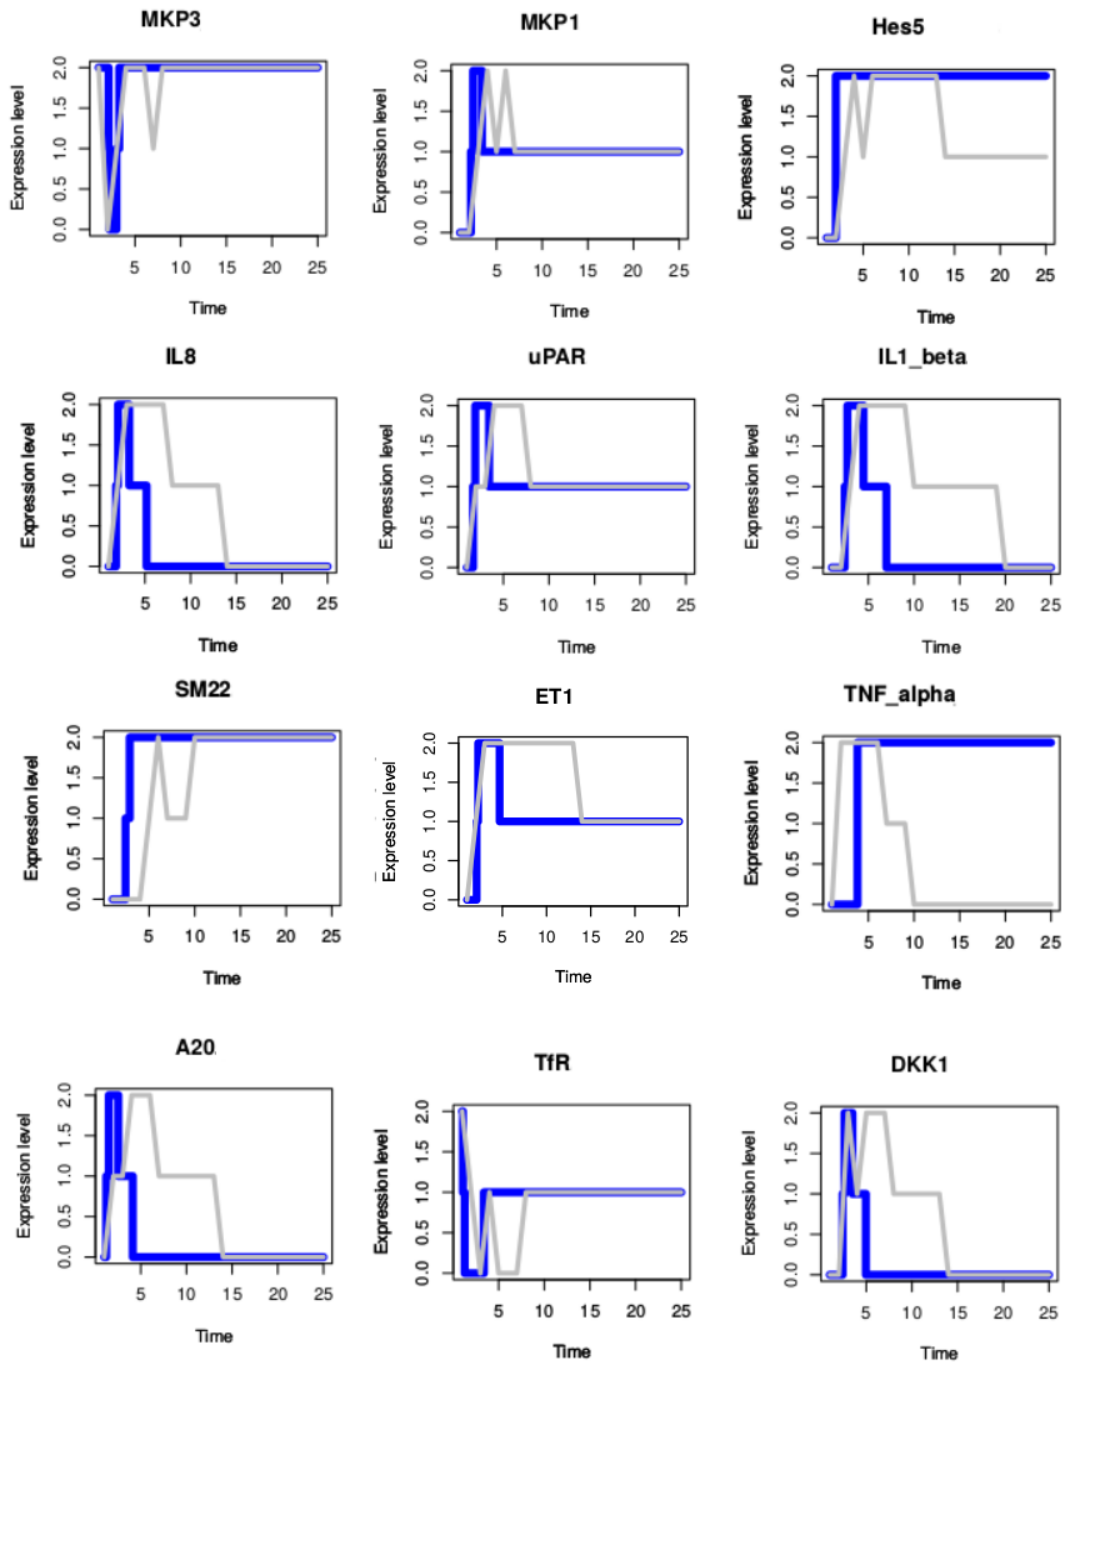
\includegraphics[scale=0.15]{figs/12genes_sim.png}
\end{center}

\textbf{Simulations}

\begin{itemize}
  \item For $r_{a} = r_{i}=10.0$ et $sa = 50 $ for all signalling proteins
  \item With estimated $r$ and $sa$ for MKP3, MKP1, uPAR, Hes5,... according to their expression profiles
  
\end{itemize}

%\textcolor{couleurtheme}{$\Rightarrow$} \fbox{\tval{\large Analyse???}} \textcolor{couleurtheme}{$\Leftarrow$}

\end{frame}




\begin{frame}[c]
  \frametitle{Simulations and analysis}
  
 \begin{center}
  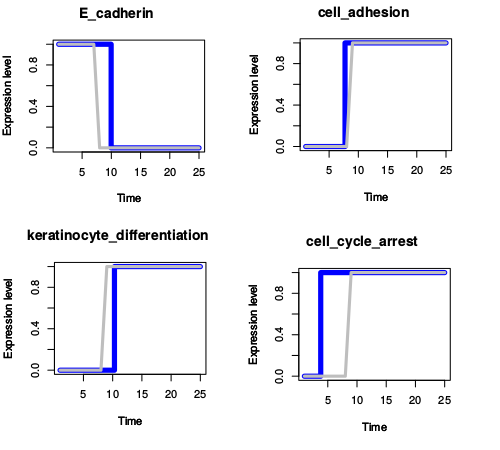
\includegraphics[scale=0.35]{figs/key_nodes1.png}
\end{center}

\textbf{Simulations}

\begin{itemize}
  \item Input node of the system (E\_cadherin)
 \item For biological processes (Cell adhesion, Cell cycle arrest, Keratinocyte differentiation)
  
\end{itemize}

%\textcolor{couleurtheme}{$\Rightarrow$} \fbox{\tval{\large Analyse???}} \textcolor{couleurtheme}{$\Leftarrow$}

\end{frame}

%\begin{frame}
   \frametitle{Simulation and Trace analysis}
   %\framesubtitle{work with Guillaume Taupiac}


\begin{columns}
\begin{column}{0.5\textwidth}

\scalebox{0.9}{
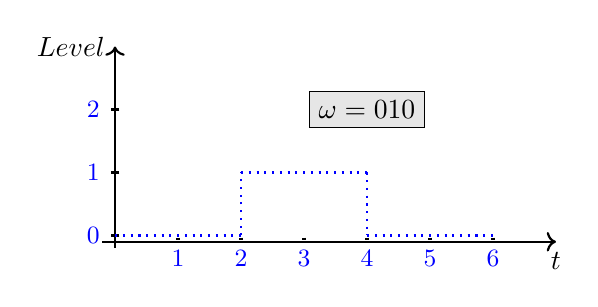
\begin{tikzpicture}[scale = 0.8]
       
    \draw[thick, ->] (-.2,-.1)--(7,-.1) node[below]{$t$};
     \foreach \t in {1,2,3,4,5,6}
      \draw[very thick] (\t,-1pt)--(\t,-2pt) node[below,blue]{\small\t};

     \draw[thick, ->] (0,-.2)--(0,3) node[left]{$Level$};
     \foreach \y in {0,1,2}
      \draw[very thick] (2pt,\y)--(-2pt,\y) node[left,blue]{\small\y};
    
    
    \draw[thick,dotted,blue] (0,0) -- (2,0) node[below]{}; 
    \draw[thick,dotted,blue] (2,0) -- (2,1) node[below]{}; 
    \draw[thick,dotted,blue] (2,1) -- (4,1) node[below]{};
    \draw[thick,dotted,blue] (4,1) -- (4,0) node[below]{};
    \draw[thick,dotted,blue] (4,0) -- (6,0) node[below]{};
    \node[instruct,align=center] (mot2) at (4,2) {$\omega=010$};

\end{tikzpicture}
}


%deuxième exemple 
\scalebox{0.9}{
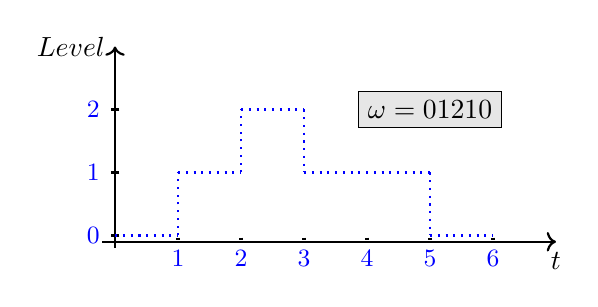
\begin{tikzpicture}[scale = 0.8]
       
    \draw[thick, ->] (-.2,-.1)--(7,-.1) node[below]{$t$};
     \foreach \t in {1,2,3,4,5,6}
      \draw[very thick] (\t,-1pt)--(\t,-2pt) node[below,blue]{\small \t};

     \draw[thick, ->] (0,-.2)--(0,3) node[left]{$Level$};
     \foreach \y in {0,1,2}
      \draw[very thick] (2pt,\y)--(-2pt,\y) node[left,blue]{\small \y};
    
    
    \draw[thick,dotted,blue] (0,0) -- (1,0) node[below]{}; 
    \draw[thick,dotted,blue] (1,0) -- (1,1) node[below]{}; 
    \draw[thick,dotted,blue] (1,1) -- (2,1) node[below]{};
    \draw[thick,dotted,blue] (2,1) -- (2,2) node[below]{};
    \draw[thick,dotted,blue] (2,2) -- (3,2) node[below]{};
    \draw[thick,dotted,blue] (3,2) -- (3,1) node[below]{};
    \draw[thick,dotted,blue] (3,1) -- (5,1) node[below]{};
    \draw[thick,dotted,blue] (5,1) -- (5,0) node[below]{};
    \draw[thick,dotted,blue] (5,0) -- (6,0) node[below]{};
    \node[instruct,align=center] (mot2) at (5,2) {$\omega=01210$};
   

\end{tikzpicture}
}


\end{column}


\begin{column}{0.5\textwidth}

for each component \tval{$C_{i}$, $1 \leq i \leq P$},
\tval{$N$} simulations will generate \tval{$\omega_{i1}, \omega_{i2}, \ldots ,\omega_{iN}$} words.




for $1 \leq j \leq N$

%\newline
%\vspace{1cm}



\scalebox{0.9}{
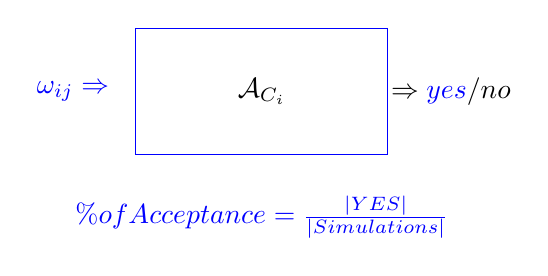
\begin{tikzpicture}[scale = 0.8]
    
    \node[align=center,blue] (mot) at (2,3) {$\omega_{ij} \Rightarrow $};
    
    \draw[blue] (3,2) rectangle (7,4);

    \node[align=center] (automaton) at (5,3) {$\mathcal{A}_{C_{i}}$};
    
    \node[align=center] (accept) at (8,3) {$\Rightarrow \tval{yes}/\alert{no} $};
    
    \node[align=center] (percent) at (5,1) {\tval{$\% of Acceptance = \frac{\card{YES}}{\card{Simulations}}$}};
   

\end{tikzpicture}
}



\end{column}
\end{columns}
\end{frame}

\begin{frame}
\frametitle{Simulation and Trace analysis}
\begin{tabular}{|c|c||c|c|}
\hline

\textbf{Automate} & \textbf{components} & \textbf{$\%$  validation} & \textbf{$\%$ of acceptance $T_{1}$}
\\ \hline

$\mathcal{A}_{2}(01210)$ & A20 & 91 & 100 
\\ \hline

$\mathcal{A}_{2}(01210)$ & IL1$\_$beta & 81 & 100
\\ \hline

$\mathcal{A}_{2}(01210)$ & IL8 & 93 & 100 
\\ \hline

$\mathcal{A}_{2}(01210)$ & TNF$\_$alpha & 0 & 0
\\ \hline

$\mathcal{A}_{3}(01211)$ & uPar & 76 & 99 
\\ \hline

$\mathcal{A}_{3}(01211)$ & ET1 & 8 & 19 
\\ \hline

$\mathcal{A}_{4}(0121210)$ & DKK1 & 13 & 43

\\ \hline

$\mathcal{A}_{5}(0121211)$ & Hes5 & 0 & 17 
\\ \hline

$\mathcal{A}_{5}(0121211)$ & MKP1 & 9 & 97
\\ \hline

$\mathcal{A}_{6}(0212)$ & SM22 & 11 & 100 
\\ \hline

$\mathcal{A}_{7}(02010)$ & MKP3 & 11 & 98

\\ \hline

$\mathcal{A}_{8}(02121)$ & Tfr & 0 & 94 
\\ \hline

\end{tabular}

\end{frame}



\begin{comment}
\begin{frame}
   \frametitle{Simulation and Trace analysis}
   %\framesubtitle{work with Guillaume Taupiac}


\begin{columns}
\begin{column}{0.5\textwidth}

\scalebox{0.9}{
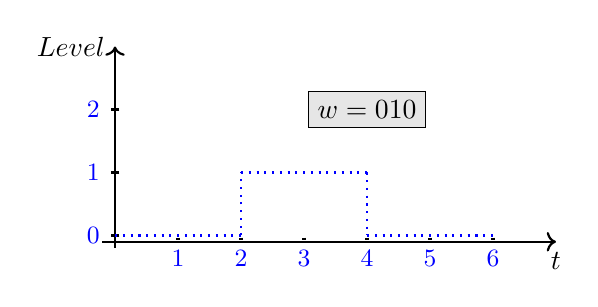
\begin{tikzpicture}[scale = 0.8]
       
    \draw[thick, ->] (-.2,-.1)--(7,-.1) node[below]{$t$};
     \foreach \t in {1,2,3,4,5,6}
      \draw[very thick] (\t,-1pt)--(\t,-2pt) node[below,blue]{\small\t};

     \draw[thick, ->] (0,-.2)--(0,3) node[left]{$Level$};
     \foreach \y in {0,1,2}
      \draw[very thick] (2pt,\y)--(-2pt,\y) node[left,blue]{\small\y};
    
    
    \draw[thick,dotted,blue] (0,0) -- (2,0) node[below]{}; 
    \draw[thick,dotted,blue] (2,0) -- (2,1) node[below]{}; 
    \draw[thick,dotted,blue] (2,1) -- (4,1) node[below]{};
    \draw[thick,dotted,blue] (4,1) -- (4,0) node[below]{};
    \draw[thick,dotted,blue] (4,0) -- (6,0) node[below]{};
    \node[instruct,align=center] (mot2) at (4,2) {$w=010$};

\end{tikzpicture}
}


%deuxième exemple 
\scalebox{0.9}{
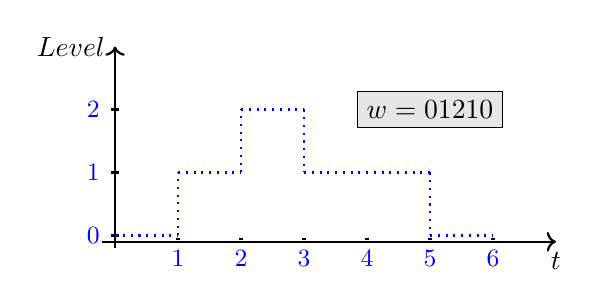
\begin{tikzpicture}[scale = 0.8]
       
    \draw[thick, ->] (-.2,-.1)--(7,-.1) node[below]{$t$};
     \foreach \t in {1,2,3,4,5,6}
      \draw[very thick] (\t,-1pt)--(\t,-2pt) node[below,blue]{\small \t};

     \draw[thick, ->] (0,-.2)--(0,3) node[left]{$Level$};
     \foreach \y in {0,1,2}
      \draw[very thick] (2pt,\y)--(-2pt,\y) node[left,blue]{\small \y};
    
    
    \draw[thick,dotted,blue] (0,0) -- (1,0) node[below]{}; 
    \draw[thick,dotted,blue] (1,0) -- (1,1) node[below]{}; 
    \draw[thick,dotted,blue] (1,1) -- (2,1) node[below]{};
    \draw[thick,dotted,blue] (2,1) -- (2,2) node[below]{};
    \draw[thick,dotted,blue] (2,2) -- (3,2) node[below]{};
    \draw[thick,dotted,blue] (3,2) -- (3,1) node[below]{};
    \draw[thick,dotted,blue] (3,1) -- (5,1) node[below]{};
    \draw[thick,dotted,blue] (5,1) -- (5,0) node[below]{};
    \draw[thick,dotted,blue] (5,0) -- (6,0) node[below]{};
    \node[instruct,align=center] (mot2) at (5,2) {$w=01210$};
   

\end{tikzpicture}
}


\end{column}


\begin{column}{0.5\textwidth}

\begin{tabular}{|c|c||c|c|}
\hline

\textbf{Automate}

&

\textbf{components}

&

\textbf{$\%$  validation}

&

\textbf{$\%$ of acceptance $T_{1}$}
\\ \hline

$\mathcal{A}_{2}(01210)$

&

A20

&

91

&

100
\\ \hline

$\mathcal{A}_{2}(01210)$

&

IL1$\_$beta

&

81

&

100
\\ \hline

$\mathcal{A}_{2}(01210)$

&

IL8

&

93

&

100

\\ \hline

$\mathcal{A}_{2}(01210)$

&

TNF$\_$alpha

&

0

&

0

\\ \hline

$\mathcal{A}_{3}(01211)$

&

uPar

&

76

&

99

\\ \hline

$\mathcal{A}_{3}(01211)$

&

ET1

&

8

&

19

\\ \hline

$\mathcal{A}_{4}(0121210)$

&

DKK1

&

13

&

43

\\ \hline

$\mathcal{A}_{5}(0121211)$

&

Hes5


&

0

&

17

\\ \hline

$\mathcal{A}_{5}(0121211)$

&

MKP1


&

9

&

97

\\ \hline

$\mathcal{A}_{6}(0212)$

&

SM22


&

11

&

100

\\ \hline

$\mathcal{A}_{7}(02010)$

&

MKP3


&

11

&

98

\\ \hline

$\mathcal{A}_{8}(02121)$

&

Tfr


&

0

&

94

\\ \hline

 
\end{tabular}


\end{column}
\end{columns}
\end{frame}
\end{comment}

%%mettre une transition
%\section{Static analysis of quantitative properties in Stochastic Automata Networks}
%\subsection{Stochastic Automata Networks}
%% Définition du Process Hitting + sortes coopératives

%san presentation
\begin{comment}
\begin{frame}
\frametitle{Biological networks modelling}
\begin{tikzpicture}
\node (brn) at (0,5) {\begin{tikzpicture}[auto,scale=0.9] 
                                                 \path[use as bounding box] (-0.7,-0.3) rectangle (2.5,2);

                                                              \node[qgre,scale=0.8] (a) at (0,2) {a};
                                                              \node[mod,scale=0.8] (i) at (1,1) {i};
                                                              \node[qgre,scale=0.8] (b) at (0,0) {b};
                                                              \node[qgre,scale=0.8] (c) at (2,1) {c};
                                                              \path
                                                                (a) edge[inh,scale=0.1] (i)
                                                                (b) edge[act,scale=0.1] (i)
                                                                (i) edge[st,scale=0.1]  (c);
                                                              
                                                 \end{tikzpicture}};
\node[scale=0.6] (an) at (7,5) {\begin{tikzpicture}
\exandef
\end{tikzpicture}};
\node[scale=0.6] (sg) at (2,1) {
\begin{tikzpicture}[line join=bevel,font=\LARGE]
%%
  \node (6) at (405.0bp,18.0bp) [reach,nd4] {$\langle a_2,b_1,c_0\rangle$};
  \node (2) at (405.0bp,90.0bp) [reach,nd3] {$\langle a_2,b_0,c_0\rangle$};
  \node (1) at (570.0bp,90.0bp) [reach,nd1] {$\langle a_1,b_0,c_0\rangle$};
  \node (0) at (469.0bp,162.0bp) [reach,nd0] {$s_0 = \langle a_0,b_0,c_0\rangle$};
  \node (4) at (469.0bp,234.0bp) [reach,nd5] {$\langle a_0,b_1,c_0\rangle$};
 
 
  \draw [->,arc3] (0) ..controls (445.65bp,135.46bp) and (435.95bp,124.86bp)  .. (2);
  \draw [->,arc5] (0) ..controls (475.71bp,188.03bp) and (475.94bp,197.36bp)  .. (4);
  \draw [->,arc4] (2) ..controls (405.0bp,63.983bp) and (405.0bp,54.712bp)  .. (6);
  \draw [->,arc1] (0) ..controls (499.93bp,134.79bp) and (517.41bp,122.58bp)  .. (1);
  \draw [->,arc2] (1) ..controls (539.0bp,117.26bp) and (521.52bp,129.47bp)  .. (0);
  \draw [->,arc5] (4) ..controls (462.3bp,208.35bp) and (462.06bp,199.03bp)  .. (0);
 
%
\end{tikzpicture}

};
\path 
(brn) edge[->,line width=8pt, color=lightgray] (an)
(an) edge[->,line width=8pt, color=lightgray,bend left] (sg)
;

\end{tikzpicture}
\end{frame}
\end{comment}

\begin{frame}
  \frametitle{Stochastic Automata Networks}
  %\framesubtitle{\tcite{Paulev\'e et al. 2012}}
\begin{columns}
\begin{column}{0.6\textwidth}

% Automate sans les rates
\only<1->{
\tikzstyle{tick}=[densely dotted]
\tikzstyle{hit}=[->,>=angle 45]
\tikzstyle{selfhit}=[min distance=30pt,curve to]
\tikzstyle{bounce}=[densely dotted,>=stealth',->]
\tikzstyle{hlhit}=[very thick]
\begin{center}\scalebox{\scaleex}{
\begin{tikzpicture}
\exandef
\end{tikzpicture}
}\end{center}
}
\end{column}

\begin{column}{0.4\textwidth}
\begin{figure}[p]
\centering

\scalebox{0.4}{

\only<1->{
\tikzstyle{arc0}=[->]
\tikzstyle{nd0}=[]
\tikzstyle{arc1}=[->]
\tikzstyle{nd1}=[]
\tikzstyle{arc2}=[->]
\tikzstyle{nd2}=[]
\tikzstyle{arc3}=[->]
\tikzstyle{nd3}=[]
\tikzstyle{arc4}=[->]
\tikzstyle{nd4}=[]
\tikzstyle{arc5}=[->]
\tikzstyle{nd5}=[]

\begin{tikzpicture}[line join=bevel,font=\LARGE]
%%
  \node (6) at (405.0bp,18.0bp) [reach,nd4] {$\langle a_2,b_1,c_0\rangle$};
  \node (2) at (405.0bp,90.0bp) [reach,nd3] {$\langle a_2,b_0,c_0\rangle$};
  \node (1) at (570.0bp,90.0bp) [reach,nd1] {$\langle a_1,b_0,c_0\rangle$};
  \node (0) at (469.0bp,162.0bp) [reach,nd0] {$s_0 = \langle a_0,b_0,c_0\rangle$};
  \node (4) at (469.0bp,234.0bp) [reach,nd5] {$\langle a_0,b_1,c_0\rangle$};
 
 
  \draw [->,arc3] (0) ..controls (445.65bp,135.46bp) and (435.95bp,124.86bp)  .. (2);
  \draw [->,arc5] (0) ..controls (475.71bp,188.03bp) and (475.94bp,197.36bp)  .. (4);
  \draw [->,arc4] (2) ..controls (405.0bp,63.983bp) and (405.0bp,54.712bp)  .. (6);
  \draw [->,arc1] (0) ..controls (499.93bp,134.79bp) and (517.41bp,122.58bp)  .. (1);
  \draw [->,arc2] (1) ..controls (539.0bp,117.26bp) and (521.52bp,129.47bp)  .. (0);
  \draw [->,arc5] (4) ..controls (462.3bp,208.35bp) and (462.06bp,199.03bp)  .. (0);
 
%
\end{tikzpicture}


}
}

\end{figure}

\end{column}
\end{columns}

\begin{liste}
  \item \tval{Automata}: components \qex{$a$, $b$, $c$}
  \item \tval{local states}: levels of expression \qex{$c_0$, $c_1$, $c_2$}
  \item \tval{States}: sets of active local states%
  \only<1->{\qex{$\PHetat{a_2, b_1, c_0}$}}
  \item \tval{Transitions}: dynamics \qex{\only<1->{$t_1 = \trans{a_0}{a_1}{b_0}$}, \only<1->{$t_2 = \trans{a_1}{a_0}{}$}, \only<1->{$t_3 = \trans{a_0}{a_2}{b_0,c_0}$}, \only<1->{$t_4 = \trans{b_0}{b_1}{}$}}
\end{liste}
\end{frame}

\begin{frame}
  \frametitle{Stochastic Automata Networks}
  %\framesubtitle{\tcite{Paulev\'e et al. 2012}}
\begin{columns}
\begin{column}{0.6\textwidth}

% Automate avec les rates
\only<1->{
\tikzstyle{tick}=[densely dotted]
\tikzstyle{hit}=[->,>=angle 45]
\tikzstyle{selfhit}=[min distance=30pt,curve to]
\tikzstyle{bounce}=[densely dotted,>=stealth',->]
\tikzstyle{hlhit}=[very thick]
\begin{center}\scalebox{\scaleex}{
\begin{tikzpicture}
\exsandef
\end{tikzpicture}
}\end{center}
}
\end{column}

\begin{column}{0.4\textwidth}
\begin{figure}[p]
\centering

\scalebox{0.4}{

\only<1->{
\tikzstyle{arc0}=[->]
\tikzstyle{nd0}=[]
\tikzstyle{arc1}=[->]
\tikzstyle{nd1}=[]
\tikzstyle{arc2}=[->]
\tikzstyle{nd2}=[]
\tikzstyle{arc3}=[->]
\tikzstyle{nd3}=[]
\tikzstyle{arc4}=[->]
\tikzstyle{nd4}=[]
\tikzstyle{arc5}=[->]
\tikzstyle{nd5}=[]

\begin{tikzpicture}[line join=bevel,font=\LARGE]
%%
  \node (6) at (405.0bp,18.0bp) [reach,nd4] {$\langle a_2,b_1,c_0\rangle$};
  \node (2) at (405.0bp,90.0bp) [reach,nd3] {$\langle a_2,b_0,c_0\rangle$};
  \node (1) at (570.0bp,90.0bp) [reach,nd1] {$\langle a_1,b_0,c_0\rangle$};
  \node (0) at (469.0bp,162.0bp) [reach,nd0] {$s_0 = \langle a_0,b_0,c_0\rangle$};
  \node (4) at (469.0bp,234.0bp) [reach,nd5] {$\langle a_0,b_1,c_0\rangle$};
 
 
  \draw [->,arc3] (0) ..controls (445.65bp,135.46bp) and (435.95bp,124.86bp)  .. node[auto] {$\mathbf{\color{Maroon} 2}$}(2) ;
  \draw [->,arc5] (0) ..controls (475.71bp,188.03bp) and (475.94bp,197.36bp)  .. node[right] {$\mathbf{\color{Maroon} 3}$}(4) ;
  \draw [->,arc4] (2) ..controls (405.0bp,63.983bp) and (405.0bp,54.712bp)  .. node[auto] {$\mathbf{\color{Maroon} 3}$}(6) ;
  \draw [->,arc1] (0) ..controls (499.93bp,134.79bp) and (517.41bp,122.58bp)  .. node[auto] {$\mathbf{\color{Maroon} 1}$}(1) ;
  \draw [->,arc2] (1) ..controls (539.0bp,117.26bp) and (521.52bp,129.47bp)  .. node[auto] {$\mathbf{\color{Maroon} 2}$}(0) ;
  \draw [->,arc5] (4) ..controls (462.3bp,208.35bp) and (462.06bp,199.03bp)  .. node[left] {$\mathbf{\color{Maroon} 1}$}(0) ;
 
%
\end{tikzpicture}


}
}

\end{figure}

\end{column}
\end{columns}

\begin{liste}
  \item \tval{Automata}: components \qex{$a$, $b$, $c$}
  \item \tval{local states}: levels of expression \qex{$c_0$, $c_1$, $c_2$}
  \item \tval{States}: sets of active local states%
  \only<1->{\qex{$\PHetat{a_2, b_1, c_0}$}}
  \item \tval{Transitions}: dynamics \qex{\only<1->{$t_1 = \trans{a_0}{a_1}{b_0,\mathbf{\color{Maroon} 2}}$}, \only<1->{$t_2 = \trans{a_1}{a_0}{\mathbf{\color{Maroon} 1}}$}, \only<1->{$t_3 = \trans{a_0}{a_2}{b_0,c_0,\mathbf{\color{Maroon} 2}}$}, \only<1->{$t_4 = \trans{b_0}{b_1}{\mathbf{\color{Maroon} 3}}$}}
\end{liste}
\end{frame}

\begin{frame}
\frametitle{SAN as CTMC}
\begin{figure}[p]
\centering
\scalebox{0.4}{

\begin{tikzpicture}[line join=bevel,font=\LARGE]
%%
  \node (6) at (405.0bp,18.0bp) [reach] {$\langle \mathbf{\color{blue}a_2},b_1,c_0\rangle$};
  \node (2) at (405.0bp,90.0bp) [reach] {$\langle \mathbf{\color{blue}a_2},b_0,c_0\rangle$};

\node (1) at (570.0bp,90.0bp) [reach] {$\langle a_1,b_0,c_0\rangle$};
  \node (64) at (304.0bp,234.0bp) [reach] {$\langle a_0,b_0,c_1\rangle$};
  \node (0) at (469.0bp,162.0bp) [reach] {$\langle a_0,b_0,c_0\rangle}$};
  \node (5) at (507.0bp,306.0bp) [reach] {$\langle a_1,b_1,c_0\rangle$};
  \node (4) at (469.0bp,234.0bp) [reach] {$\langle a_0,b_1,c_0\rangle$};
  \node (69) at (425.0bp,378.0bp) [reach] {$\mathbf{\color{Maroon}s =\langle a_1,b_1,c_1\rangle$};
  \node (68) at (342.0bp,306.0bp) [reach] {$\langle a_0,b_1,c_1\rangle$};
  \node (65) at (232.0bp,450.0bp) [reach] {$\langle a_1,b_0,c_1\rangle$};

  \node[elipse,fill=gray!30] (129) at (88.0bp,90.0bp)  {$\langle a_1,b_0,c_2\rangle$};
  \node[elipse,fill=gray!30] (128) at (139.0bp,162.0bp)  {$\langle a_0,b_0,c_2\rangle$};
  \node[elipse,fill=gray!30] (133) at (112.0bp,306.0bp)  {$\langle a_1,b_1,c_2\rangle$};
  \node[elipse,fill=gray!30] (132) at (139.0bp,234.0bp)  {$\langle a_0,b_1,c_2\rangle$};

  \draw [->] (0) ..controls (445.65bp,135.46bp) and (435.95bp,124.86bp)  .. node[auto] {$\mathbf{\color{Maroon} 2}$}(2);
  \draw [->] (133) ..controls (121.57bp,280.18bp) and (125.26bp,270.62bp)  .. node[auto] {$\mathbf{\color{Maroon} 1}$}(132);
  \draw [->] (65) ..controls (104.12bp,424.19bp) and (0.0bp,387.99bp)  ..  (0.0bp,307.0bp) .. controls (0.0bp,307.0bp) and (0.0bp,307.0bp)  ..  node[auto] {$\mathbf{\color{Maroon} 2}$} (0.0bp,233.0bp) .. controls (0.0bp,185.75bp) and (35.64bp,141.13bp)  .. node[auto] {$\mathbf{\color{Maroon} 3}$}(129);
  \draw [->] (65) ..controls (223.97bp,401.24bp) and (228.52bp,336.68bp)  .. (251.0bp,288.0bp) .. controls (255.96bp,277.25bp) and (263.67bp,266.89bp)  .. node[auto] {$\mathbf{\color{Maroon} 1}$}(64);
  \draw [->] (5) ..controls (483.32bp,333.07bp) and (470.02bp,344.55bp)  .. node[auto] {$\mathbf{\color{Maroon} 2}$}(69);
  \draw [->] (64) ..controls (244.15bp,207.61bp) and (210.57bp,193.36bp)  .. node[auto] {$\mathbf{\color{Maroon} 2}$} (128);
  \draw [->] (5) ..controls (493.43bp,280.01bp) and (488.11bp,270.2bp)  .. node[auto] {$\mathbf{\color{Maroon} 1}$}(4);
  \draw [->] (0) ..controls (475.71bp,188.03bp) and (475.94bp,197.36bp)  .. node[right] {$\mathbf{\color{Maroon} 3}$}(4);
  \draw [->] (1) ..controls (588.79bp,134.38bp) and (608.0bp,186.55bp)  .. (608.0bp,233.0bp) .. controls (608.0bp,307.0bp) and (608.0bp,307.0bp)  .. (608.0bp,307.0bp) .. controls (608.0bp,366.83bp) and (560.73bp,369.68bp)  .. (507.0bp,396.0bp) .. controls (446.14bp,425.81bp) and (370.03bp,438.87bp)  .. node[auto] {$\mathbf{\color{Maroon} 3}$}(65);
  \draw [->] (1) ..controls (572.33bp,138.66bp) and (571.97bp,203.11bp)  .. (551.0bp,252.0bp) .. controls (546.57bp,262.33bp) and (539.46bp,272.21bp)  .. node[right] {$\mathbf{\color{Maroon} 3}$}(5);
  \draw [->] (129) ..controls (68.077bp,117.99bp) and (60.513bp,131.04bp)  .. (57.0bp,144.0bp) .. controls (44.446bp,190.33bp) and (38.221bp,207.83bp)  .. (57.0bp,252.0bp) .. controls (61.945bp,263.63bp) and (70.831bp,273.95bp)  .. node[auto] {$\mathbf{\color{Maroon} 3}$}(133);
  \draw [->] (128) ..controls (145.71bp,188.03bp) and (145.94bp,197.36bp)  .. node[right] {$\mathbf{\color{Maroon} 3}$}(132);
  \draw [->] (69) ..controls (448.8bp,350.83bp) and (462.16bp,339.29bp)  .. node[auto] {$\mathbf{\color{Maroon} 3}$}(5);
  \draw [->] (2) ..controls (405.0bp,63.983bp) and (405.0bp,54.712bp)  .. node[auto] {$\mathbf{\color{Maroon} 3}$}(6);
  \draw [->] (0) ..controls (499.93bp,134.79bp) and (517.41bp,122.58bp)  .. node[auto] {$\mathbf{\color{Maroon} 1}$}(1);
  \draw [->] (68) ..controls (388.56bp,279.34bp) and (412.1bp,266.36bp)  .. node[auto] {$\mathbf{\color{Maroon} 1}$}(4);
  \draw [->] (68) ..controls (321.75bp,280.09bp) and (316.27bp,270.41bp)  .. node[auto] {$\mathbf{\color{Maroon} 3}$}(64);
  \draw [->] (1) ..controls (539.0bp,117.26bp) and (521.52bp,129.47bp)  .. node[auto] {$\mathbf{\color{Maroon} 2}$}(0);
  \draw [->] (65) ..controls (301.71bp,423.72bp) and (343.47bp,408.57bp)  .. node[auto] {$\mathbf{\color{Maroon} 3}$}(69);
  \draw [->] (64) ..controls (324.32bp,260.04bp) and (329.77bp,269.67bp)  .. node[auto] {$\mathbf{\color{Maroon} 1}$}(68);
  \draw [->] (69) ..controls (394.58bp,351.34bp) and (381.1bp,339.97bp)  .. node[auto] {$\mathbf{\color{Maroon} 1}$}(68);
  \draw [->] (128) ..controls (114.09bp,136.08bp) and (106.38bp,125.8bp)  .. node[auto] {$\mathbf{\color{Maroon} 1}$}(129);
  \draw [->] (64) ..controls (285.73bp,261.68bp) and (275.22bp,274.54bp)  .. (269.0bp,288.0bp) .. controls (248.81bp,331.74bp) and (243.08bp,388.29bp)  .. node[auto] {$\mathbf{\color{Maroon} 2}$}(65);
  \draw [->] (132) ..controls (132.3bp,208.35bp) and (132.06bp,199.03bp)  .. node[auto] {$\mathbf{\color{Maroon} 1}$}(128);
  \draw [->] (4) ..controls (462.3bp,208.35bp) and (462.06bp,199.03bp)  .. node[left] {$\mathbf{\color{Maroon} 1}$}(0);
  \draw [->] (129) ..controls (113.05bp,116.11bp) and (120.71bp,126.32bp)  .. node[auto] {$\mathbf{\color{Maroon} 2}$}(128);
%
\end{tikzpicture}


}

\label{ex-bifurcations}
\end{figure}
Bad news: \textcolor{red}{state space explosion}
\end{frame}

\begin{frame}
\frametitle{SAN as CTMC}
\begin{columns}
 \begin{column}{0.5\textwidth}
 \begin{figure}[p]
\centering
\scalebox{0.25}{

\begin{tikzpicture}[line join=bevel,font=\LARGE]
%%
  \node (6) at (405.0bp,18.0bp) [reach] {$\langle \mathbf{\color{blue}a_2},b_1,c_0\rangle$};
  \node (2) at (405.0bp,90.0bp) [reach] {$\langle \mathbf{\color{blue}a_2},b_0,c_0\rangle$};

\node (1) at (570.0bp,90.0bp) [reach] {$\langle a_1,b_0,c_0\rangle$};
  \node (64) at (304.0bp,234.0bp) [reach] {$\langle a_0,b_0,c_1\rangle$};
  \node (0) at (469.0bp,162.0bp) [reach] {$\langle a_0,b_0,c_0\rangle}$};
  \node (5) at (507.0bp,306.0bp) [reach] {$\langle a_1,b_1,c_0\rangle$};
  \node (4) at (469.0bp,234.0bp) [reach] {$\langle a_0,b_1,c_0\rangle$};
  \node (69) at (425.0bp,378.0bp) [reach] {$\mathbf{\color{Maroon}s =\langle a_1,b_1,c_1\rangle$};
  \node (68) at (342.0bp,306.0bp) [reach] {$\langle a_0,b_1,c_1\rangle$};
  \node (65) at (232.0bp,450.0bp) [reach] {$\langle a_1,b_0,c_1\rangle$};

  \node[elipse,fill=gray!30] (129) at (88.0bp,90.0bp)  {$\langle a_1,b_0,c_2\rangle$};
  \node[elipse,fill=gray!30] (128) at (139.0bp,162.0bp)  {$\langle a_0,b_0,c_2\rangle$};
  \node[elipse,fill=gray!30] (133) at (112.0bp,306.0bp)  {$\langle a_1,b_1,c_2\rangle$};
  \node[elipse,fill=gray!30] (132) at (139.0bp,234.0bp)  {$\langle a_0,b_1,c_2\rangle$};

  \draw [->] (0) ..controls (445.65bp,135.46bp) and (435.95bp,124.86bp)  .. node[auto] {$\mathbf{\color{Maroon} 2}$}(2);
  \draw [->] (133) ..controls (121.57bp,280.18bp) and (125.26bp,270.62bp)  .. node[auto] {$\mathbf{\color{Maroon} 1}$}(132);
  \draw [->] (65) ..controls (104.12bp,424.19bp) and (0.0bp,387.99bp)  ..  (0.0bp,307.0bp) .. controls (0.0bp,307.0bp) and (0.0bp,307.0bp)  ..  node[auto] {$\mathbf{\color{Maroon} 2}$} (0.0bp,233.0bp) .. controls (0.0bp,185.75bp) and (35.64bp,141.13bp)  .. node[auto] {$\mathbf{\color{Maroon} 3}$}(129);
  \draw [->] (65) ..controls (223.97bp,401.24bp) and (228.52bp,336.68bp)  .. (251.0bp,288.0bp) .. controls (255.96bp,277.25bp) and (263.67bp,266.89bp)  .. node[auto] {$\mathbf{\color{Maroon} 1}$}(64);
  \draw [->] (5) ..controls (483.32bp,333.07bp) and (470.02bp,344.55bp)  .. node[auto] {$\mathbf{\color{Maroon} 2}$}(69);
  \draw [->] (64) ..controls (244.15bp,207.61bp) and (210.57bp,193.36bp)  .. node[auto] {$\mathbf{\color{Maroon} 2}$} (128);
  \draw [->] (5) ..controls (493.43bp,280.01bp) and (488.11bp,270.2bp)  .. node[auto] {$\mathbf{\color{Maroon} 1}$}(4);
  \draw [->] (0) ..controls (475.71bp,188.03bp) and (475.94bp,197.36bp)  .. node[right] {$\mathbf{\color{Maroon} 3}$}(4);
  \draw [->] (1) ..controls (588.79bp,134.38bp) and (608.0bp,186.55bp)  .. (608.0bp,233.0bp) .. controls (608.0bp,307.0bp) and (608.0bp,307.0bp)  .. (608.0bp,307.0bp) .. controls (608.0bp,366.83bp) and (560.73bp,369.68bp)  .. (507.0bp,396.0bp) .. controls (446.14bp,425.81bp) and (370.03bp,438.87bp)  .. node[auto] {$\mathbf{\color{Maroon} 3}$}(65);
  \draw [->] (1) ..controls (572.33bp,138.66bp) and (571.97bp,203.11bp)  .. (551.0bp,252.0bp) .. controls (546.57bp,262.33bp) and (539.46bp,272.21bp)  .. node[right] {$\mathbf{\color{Maroon} 3}$}(5);
  \draw [->] (129) ..controls (68.077bp,117.99bp) and (60.513bp,131.04bp)  .. (57.0bp,144.0bp) .. controls (44.446bp,190.33bp) and (38.221bp,207.83bp)  .. (57.0bp,252.0bp) .. controls (61.945bp,263.63bp) and (70.831bp,273.95bp)  .. node[auto] {$\mathbf{\color{Maroon} 3}$}(133);
  \draw [->] (128) ..controls (145.71bp,188.03bp) and (145.94bp,197.36bp)  .. node[right] {$\mathbf{\color{Maroon} 3}$}(132);
  \draw [->] (69) ..controls (448.8bp,350.83bp) and (462.16bp,339.29bp)  .. node[auto] {$\mathbf{\color{Maroon} 3}$}(5);
  \draw [->] (2) ..controls (405.0bp,63.983bp) and (405.0bp,54.712bp)  .. node[auto] {$\mathbf{\color{Maroon} 3}$}(6);
  \draw [->] (0) ..controls (499.93bp,134.79bp) and (517.41bp,122.58bp)  .. node[auto] {$\mathbf{\color{Maroon} 1}$}(1);
  \draw [->] (68) ..controls (388.56bp,279.34bp) and (412.1bp,266.36bp)  .. node[auto] {$\mathbf{\color{Maroon} 1}$}(4);
  \draw [->] (68) ..controls (321.75bp,280.09bp) and (316.27bp,270.41bp)  .. node[auto] {$\mathbf{\color{Maroon} 3}$}(64);
  \draw [->] (1) ..controls (539.0bp,117.26bp) and (521.52bp,129.47bp)  .. node[auto] {$\mathbf{\color{Maroon} 2}$}(0);
  \draw [->] (65) ..controls (301.71bp,423.72bp) and (343.47bp,408.57bp)  .. node[auto] {$\mathbf{\color{Maroon} 3}$}(69);
  \draw [->] (64) ..controls (324.32bp,260.04bp) and (329.77bp,269.67bp)  .. node[auto] {$\mathbf{\color{Maroon} 1}$}(68);
  \draw [->] (69) ..controls (394.58bp,351.34bp) and (381.1bp,339.97bp)  .. node[auto] {$\mathbf{\color{Maroon} 1}$}(68);
  \draw [->] (128) ..controls (114.09bp,136.08bp) and (106.38bp,125.8bp)  .. node[auto] {$\mathbf{\color{Maroon} 1}$}(129);
  \draw [->] (64) ..controls (285.73bp,261.68bp) and (275.22bp,274.54bp)  .. (269.0bp,288.0bp) .. controls (248.81bp,331.74bp) and (243.08bp,388.29bp)  .. node[auto] {$\mathbf{\color{Maroon} 2}$}(65);
  \draw [->] (132) ..controls (132.3bp,208.35bp) and (132.06bp,199.03bp)  .. node[auto] {$\mathbf{\color{Maroon} 1}$}(128);
  \draw [->] (4) ..controls (462.3bp,208.35bp) and (462.06bp,199.03bp)  .. node[left] {$\mathbf{\color{Maroon} 1}$}(0);
  \draw [->] (129) ..controls (113.05bp,116.11bp) and (120.71bp,126.32bp)  .. node[auto] {$\mathbf{\color{Maroon} 2}$}(128);
%
\end{tikzpicture}


}

\label{ex-bifurcations}
\end{figure}
Bad news: \textcolor{red}{state space explosion}
  
 \end{column}
 
 \begin{column}{0.5\textwidth}
  \textbf{Probability to have a transition from state s:}
  $$\ppexit{s}{*}{t} = 1-e^{-\lambda t}$$ \\
  \medskip
  \textbf{Probability to have a transition from s to s':}
  $$\ppexit{s}{s^{'}}{t} = \frac{R (s,s^{'})}{E (s)} \cdot \ppexit{s}{*}{t}$$\\
  \medskip
  \textbf{Probability to have a transition from s to a set of states:}
  $$\ppexit{s}{A}{t} = \frac{R (s,A)}{E (s)} \cdot \ppexit{s}{*}{t}$$ \\
 \end{column}

\end{columns}

\end{frame}



%\subsection{Quantitative Abstract Interpretation}
%\begin{frame}
 \frametitle{Contribution}
 
\begin{figure}[h]
\centering
\begin{tikzpicture}[node distance=1.5cm]
\draw (-4, 0) -- (4, 0);
 % Small tickmarks on the x axis
        \foreach \x in {-4,-1.9,...,4} {
            \draw (\x, 0) -- (\x, -0.8pt);
        }
% Labels on the $x$ axis; the llap makes the label center on the
        % number without the minus.
        \foreach \x/\label in {-4/0,-2/{\color{blue}\binf{\Prob{\pacc}}},0/\Prob{\pacc},2/{\color{blue}\bsup{\Prob{\pacc}}},4/1} {
            \node[x tick label] at (\x, -0.5) {$\label$};
            \draw[major tick] (\x, 0) -- (\x, -1.25pt);
        }
\node[axis label] at (4.5,0) {$\scriptstyle \mathcal{P}$};

\end{tikzpicture}
 \end{figure}
 \hspace{5cm}
 
 \textbf{Aim:}
 \begin{itemize}
  \item Formal characterization of \tval{quantitative properties}.
  \item Static analysis of \tval{Probability} and \tval{Delay} of reachability properties.
  \item Estimate a \tval{lower bound} and an \tval{upper bound} of a quantitative properties.  
 \end{itemize}
 \textbf{Contribution:}
 $$
\left\{
    \begin{array}{lcl}
        \mbox{QS (Quotient set)} &\\  %rajouter un signe entre les deux
        \mbox{+} & \Longrightarrow \mbox{\tval{formal approximation of quantitative}} \\
        \mbox{AI (Abstract interpretation)} & \mbox{\ \ \ \ \tval{properties}}
    \end{array}
\right.
$$ 
 

\end{frame}


\begin{frame}
\frametitle{Abstract Interpretation}
\framesubtitle{Local Causality}
\begin{columns}
%l'automate
\begin{column}{0.4\textwidth}
\begin{center}\scalebox{\scaleex}{
\begin{tikzpicture}
\exanaidef
\end{tikzpicture}
}\end{center}
\end{column}
%le glc associé
\begin{column}[c]{0.6\textwidth}

local-cause($\obj{d_1}{d_2}$) = \{$\trans{d_1}{d_2}{b_1}$, $\trans{d_1}{d_2}{c_2}$\}
\medskip
local-cause^\#($\obj{d_1}{d_2}$) = $\{\{b_1\},\{c_2\}\}$ \\

\hspace*{5em}

\begin{center}\scalebox{\scaleex}{
%\begin{tikzpicture}
\exlcgaidef
%\end{tikzpicture}
}\end{center}

\end{column}
\end{columns}
\end{frame}

\begin{frame}
\frametitle{Abstract Interpretation}
\framesubtitle{Local Causality Graph}
\begin{itemize}
 \item \textbf{Initial context/state:} \qex{$\PHetat{a_0,b_0,c_1,d_1,e_1,f_0}$}
 \item \textbf{Goal:} local state {\color{blue}$d_2$}
\end{itemize}
\begin{columns}
\begin{column}{0.5\textwidth}
\begin{center}\scalebox{0.6}{
\begin{tikzpicture}
\exanppdef
\TState{1}{a_0,b_0,c_1,d_1,e_1,f_0}
\end{tikzpicture}
}\end{center}
\end{column}
\begin{column}{0.5\textwidth}
\begin{center}\scalebox{0.7}{
\exglcandef
}\end{center}
\end{column}
\end{columns}
\end{frame}

\begin{frame}
\frametitle{Abstract Interpretation}
\framesubtitle{Quantified Local Causality \& Quotient Set}
\begin{columns}
%l'automate
\begin{column}{0.3\textwidth}
\begin{left}\scalebox{\scaleex}{
\begin{tikzpicture}
\exsanaidef
\end{tikzpicture}
}\end{left}
%$$\Probt{\obj{d_1}{d_2}}(t) = \frac{3_{b_1}+2_{c_2}}{3_{b_1}+2_{c_2}+2_{e_1}}$$
\end{column}
%le glc associé
\begin{column}[c]{0.7\textwidth}

qlocal-cause($\obj{d_1}{d_2}$) = \{$\trans{d_1}{d_2}{b_1,\mathbf{\color{Maroon} 3}}$, $\trans{d_1}{d_2}{c_2,\mathbf{\color{Maroon} 2}},
{\color{red} \trans{d_1}{d_0}{e_1,\mathbf{\color{red} 2}}}$\}\\
\medskip
qlocal-cause^\#($\obj{d_1}{d_2}$) = $\{\{b_1\},\{c_2\},{\color{red}\{e_1\}}\}$ \\

$$\Probt{\obj{d_1}{d_2}}(t) =\ppexit{A_{d_1}}{A_{d_2}}{t}= \frac{R (A_{d_1},A_{d_2})}{E (A_{d_1})} \cdot \ppexit{A_{d_1}}{*}{t} $$ \\

%$\ppexit{A_{d_1}}{A_{d_2}}{t}$ \\

\hspace*{1em}
\begin{center}\scalebox{\scaleex}{
%\begin{tikzpicture}
\exqlcgaidef
%\end{tikzpicture}
}\end{center}

\end{column}
\end{columns}


\end{frame}

\begin{frame}
\frametitle{Abstract Interpretation}
\framesubtitle{Quantified Local Causality \& Quotient Set}
\begin{columns}
%l'automate
\begin{column}{0.25\textwidth}
\begin{left}\scalebox{\scaleex}{
\begin{tikzpicture}
\exsanaidef
\end{tikzpicture}
}\end{left}
%$$\Probt{\obj{d_1}{d_2}}(t) = \frac{3_{b_1}+2_{c_2}}{3_{b_1}+2_{c_2}+2_{e_1}}$$
\end{column}
%le glc associé
\begin{column}[c]{0.75\textwidth}

qlocal-cause($\obj{d_1}{d_2}$) = \{$\trans{d_1}{d_2}{b_1,\mathbf{\color{Maroon} 3}}$, $\trans{d_1}{d_2}{c_2,\mathbf{\color{Maroon} 2}},
{\color{red} \trans{d_1}{d_0}{e_1,\mathbf{\color{red} 2}}}$\}\\
\medskip
qlocal-cause^\#($\obj{d_1}{d_2}$) = $\{\{b_1\},\{c_2\},{\color{red}\{e_1\}}\}$ \\

$$\Probt{\obj{d_1}{d_2}}(t) =\ppexit{A_{d_1}}{A_{d_2}}{t}= \frac{R (A_{d_1},A_{d_2})}{E (A_{d_1})} \cdot \ppexit{A_{d_1}}{*}{t} $$ \\

$$\Probt{\obj{d_1}{d_2}}(t) = \frac{3 \cdot \Prob{b_1} + 2 \cdot \Prob{c_2}}{3 \cdot \Prob{b_1} + 2 \cdot \Prob{c_2}+ {\color{red} 2 \cdot \Prob{e_1}}}\cdot \ppexit{A_{d_1}}{*}{t}$$ \\

\textbf{Approximation:} {\color{red} $\Prob{e_1} = 1$}

% \hspace*{1em}
% \begin{center}\scalebox{\scaleex}{
% %\begin{tikzpicture}
% \exqlcgaidef
% %\end{tikzpicture}
% }\end{center}

\end{column}
\end{columns}


\end{frame}

%\subsection{Quantified Local Causality Graph}
%\begin{frame}
\frametitle{Quantified Local Causality Graph}

% \begin{columns}
%  \begin{column}{0.2\textwidth}
%   \begin{center}\scalebox{0.6}{
% \begin{tikzpicture}
% \exsanppdef
% \end{tikzpicture}
% }\end{center}
%  \end{column}
%  \begin{column}{0.8\textwidth}
 \begin{itemize}
  
 \item Probability of a \tval{node local state}:\\
 $\GProbLS{\n}{\ctx}{\cwG}{k}$\\
 \medskip
 \pause
 \item Probability of a \tval{node objective}:\\
 $\GProbObjn{\n}{\ctx}{\cwG}{k}$\\
 \medskip
 \pause
 \item Probability of a \tval{node Solution}:\\
 $\GProbSol{\n}{\ctx}{\cwG}{k}$
 \end{itemize}
 \pause
   \begin{center}\scalebox{\scaleex}{
    
    \exqlcggaidef
   
   }\end{center}
   
%  \end{column}
% \end{columns}


\end{frame}

%\subsection{Probability/Delay}
%\begin{frame}
\frametitle{Probability approximation}
\begin{columns}
 \begin{column}{0.2\textwidth}
  \begin{center}\scalebox{0.6}{
\begin{tikzpicture}
\exsanppdef
\end{tikzpicture}
}\end{center}
 \end{column}
 \begin{column}{0.8\textwidth}
 
 \only<1>{
\tikzstyle{labelproba1}=[transparent]
\tikzstyle{labelproba2}=[transparent]
\tikzstyle{labelproba3}=[transparent]
\tikzstyle{labelproba4}=[transparent]
\tikzstyle{labelproba5}=[transparent]
\tikzstyle{labelproba6}=[transparent]
\tikzstyle{labelproba7}=[transparent]
\tikzstyle{labelproba8}=[transparent]
\tikzstyle{labelproba9}=[transparent]
\tikzstyle{labelproba10}=[transparent]
\tikzstyle{labelproba11}=[transparent]
\tikzstyle{labelproba12}=[transparent]
\begin{center}\scalebox{\scaleex}{
    
    \exglcsandef
   
   }\end{center}

}
 
 \only<2>{
\tikzstyle{labelproba1}=[transparent]
\tikzstyle{labelproba2}=[transparent]
\tikzstyle{labelproba3}=[transparent]
\tikzstyle{labelproba4}=[transparent]
\tikzstyle{labelproba5}=[transparent]
\tikzstyle{labelproba6}=[transparent]
\tikzstyle{labelproba7}=[transparent]
\tikzstyle{labelproba8}=[transparent]
\tikzstyle{labelproba9}=[transparent]
\tikzstyle{labelproba10}=[transparent]
\tikzstyle{labelproba11}=[]
\tikzstyle{labelproba12}=[]
\begin{center}\scalebox{\scaleex}{
    
    \exglcsandef
   
   }\end{center}

}

 \only<3>{
\tikzstyle{labelproba1}=[transparent]
\tikzstyle{labelproba2}=[transparent]
\tikzstyle{labelproba3}=[transparent]
\tikzstyle{labelproba4}=[transparent]
\tikzstyle{labelproba5}=[transparent]
\tikzstyle{labelproba6}=[transparent]
\tikzstyle{labelproba7}=[transparent]
\tikzstyle{labelproba8}=[transparent]
\tikzstyle{labelproba9}=[]
\tikzstyle{labelproba10}=[]
\tikzstyle{labelproba11}=[]
\tikzstyle{labelproba12}=[]
\begin{center}\scalebox{\scaleex}{
    
    \exglcsandef
   
   }\end{center}

}

 \only<4>{
\tikzstyle{labelproba1}=[transparent]
\tikzstyle{labelproba2}=[transparent]
\tikzstyle{labelproba3}=[transparent]
\tikzstyle{labelproba4}=[transparent]
\tikzstyle{labelproba5}=[transparent]
\tikzstyle{labelproba6}=[transparent]
\tikzstyle{labelproba7}=[]
\tikzstyle{labelproba8}=[]
\tikzstyle{labelproba9}=[]
\tikzstyle{labelproba10}=[]
\tikzstyle{labelproba11}=[]
\tikzstyle{labelproba12}=[]
\begin{center}\scalebox{\scaleex}{
    
    \exglcsandef
   
   }\end{center}

}

 \only<5>{
\tikzstyle{labelproba1}=[transparent]
\tikzstyle{labelproba2}=[transparent]
\tikzstyle{labelproba3}=[transparent]
\tikzstyle{labelproba4}=[transparent]
\tikzstyle{labelproba5}=[]
\tikzstyle{labelproba6}=[]
\tikzstyle{labelproba7}=[]
\tikzstyle{labelproba8}=[]
\tikzstyle{labelproba9}=[]
\tikzstyle{labelproba10}=[]
\tikzstyle{labelproba11}=[]
\tikzstyle{labelproba12}=[]
\begin{center}\scalebox{\scaleex}{
    
    \exglcsandef
   
   }\end{center}

}

\only<6>{
\tikzstyle{labelproba1}=[transparent]
\tikzstyle{labelproba2}=[transparent]
\tikzstyle{labelproba3}=[]
\tikzstyle{labelproba4}=[]
\tikzstyle{labelproba5}=[]
\tikzstyle{labelproba6}=[]
\tikzstyle{labelproba7}=[]
\tikzstyle{labelproba8}=[]
\tikzstyle{labelproba9}=[]
\tikzstyle{labelproba10}=[]
\tikzstyle{labelproba11}=[]
\tikzstyle{labelproba12}=[]
\begin{center}\scalebox{\scaleex}{
    
    \exglcsandef
   
   }\end{center}

}

\only<7>{
\tikzstyle{labelproba1}=[]
\tikzstyle{labelproba2}=[]
\tikzstyle{labelproba3}=[]
\tikzstyle{labelproba4}=[]
\tikzstyle{labelproba5}=[]
\tikzstyle{labelproba6}=[]
\tikzstyle{labelproba7}=[]
\tikzstyle{labelproba8}=[]
\tikzstyle{labelproba9}=[]
\tikzstyle{labelproba10}=[]
\tikzstyle{labelproba11}=[]
\tikzstyle{labelproba12}=[]
\begin{center}\scalebox{\scaleex}{
    
    \exglcsandef
   
   }\end{center}

}

   
 \end{column}
 \end{columns}

\end{frame}

%\begin{frame}
\frametitle{Delay approximation}

\end{frame}


%%mettre une slide de transition
%\section{Static analysis of bifurcations}
%% Diapo d'intro
% \begin{frame}[c]
%   \frametitle{Context}
% %rajouter le titre (version courte) dans toute les slides
% \begin{center}
%   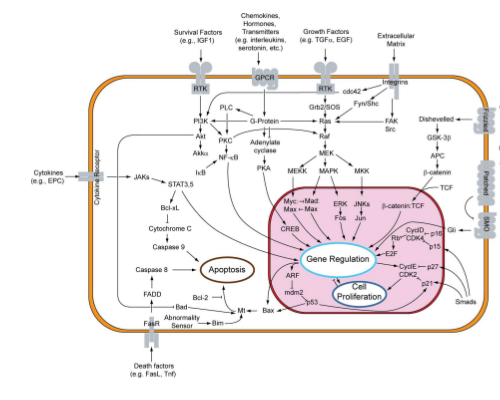
\includegraphics[scale=0.55]{images/cellule_description_lui.png}
% \end{center}
% \begin{center}
% {\tiny \color{darkgreen}[\citelui]}
% \end{center}
% 
% %\tcite{Wikipédia}
% 
% \begin{itemize}
% \item Cellular processes are driven by networks of biological interactions.
% \item Formal modelling and analysis of Biological Regulatory Network.
% \item Static analysis of properties.
% \end{itemize}
% 
% %Cellular processes are driven by networks of biological reactions. Cells rely on the tight coordination of these pathways to achieve proper functioning.
% %With the help of signaling pathway, a cell senses changes in its environnement or internal state. This information is then passed on via cascades of biochemical 
% %reactions to the appropriate mechanisms which respond by modifying the metabolic and transcriptiona activities. this in turn modifies the behavior of the cell.
% 
% %Consequently, the dynamics of biopathways play a crucial role in determinig cellular functions.
% 
% %Examples: circadian rhythm, the apoptosis pathway inducing programmed cell death, cell differentiation.
% 
% %\textcolor{couleurtheme}{$\Rightarrow$} \fbox{\tval{\large The need of comprehension of biological systems}} \textcolor{couleurtheme}{$\Leftarrow$}
% 
% 
% %\textcolor{couleurtheme}{$\Rightarrow$} \fbox{\tval{\large Allow efficient translation from Process Hitting to BRN}} \textcolor{couleurtheme}{$\Leftarrow$}
% 
% \end{frame}

\begin{frame}[c]
  \frametitle{Motivation}
 \framesubtitle{stem cell differentiation}

\begin{center}
  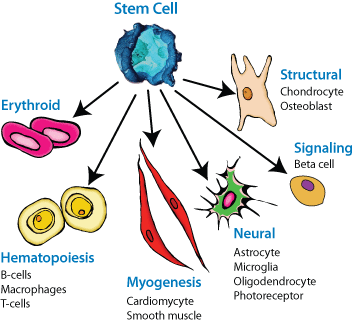
\includegraphics[scale=0.42]{images/illustration_differentiation.png}
  % \multiinclude[format=gif, scale=0.5]{images/illustration_differentiation.gif}
\end{center}
\begin{center}
{\tiny \color{darkgreen} [https://www.systembio.com/stem-cell-research/differentiation-reporters/overview]}
\end{center}
%\tcite{system Biosciences}

\begin{itemize}
\item Loss of  capability \tval{differentiation}  %expliquer la notion de perte de capacité sur la figure.
\item Which transitions (operations) are responsible of \tval{Bifurcations} ? 
\item From which state ?
\end{itemize}
\end{frame}

\begin{frame}[c]
  \frametitle{Contribution}
%system dynamique
%Bifurcations
%rajouter une autre image pour illustrer pour qu'on voit que c'est toujours des états qui changes
\begin{center}
  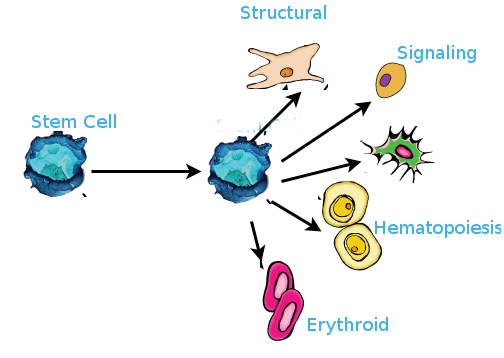
\includegraphics[scale=0.3]{images/illustration_differentiation_newio1.png}
  % \multiinclude[format=gif, scale=0.5]{images/illustration_differentiation.gif}
\end{center}


\begin{itemize}
\item Bifurcation transitions can be  expressed in temporal logic formula
\item {\bf "Relaxation"} :\\ verification of CTL formula (\tval{PSPACE (complete)})\\
       $\Rightarrow$ NP problem which can be easily expressed in SAT/ASP %trouver l'orthagraphe de easely
\item {\bf Contribution} : $$
\left\{
    \begin{array}{lcl}
        \mbox{AI (Artificial inteligence)} &\\  %rajouter un signe entre les deux
        \mbox{+} & \Longrightarrow \mbox{\tval{formal approximation of bifurcations}} \\
        \mbox{AI (Abstract interpretation)} &
    \end{array}
\right.
$$ 
\end{itemize}
\end{frame}

%\subsection{What is a bifurcation?}
%\begin{frame}[c]
 \frametitle{Illustration of bifurcations}
 
%\ref{ex-bifurcations} shows all the possible transitions from $s_0$.
\begin{figure}[p]
\centering

\scalebox{0.4}{

\begin{tikzpicture}[line join=bevel,font=\LARGE]
%%
  \node (6) at (405.0bp,18.0bp) [reach] {$\langle \mathbf{\color{blue}a_2},b_1,c_0\rangle$};
  \node (2) at (405.0bp,90.0bp) [reach] {$\langle \mathbf{\color{blue}a_2},b_0,c_0\rangle$};

\node (1) at (570.0bp,90.0bp) [reach] {$\langle a_1,b_0,c_0\rangle$};
  \node (64) at (304.0bp,234.0bp) [reach] {$\langle a_0,b_0,c_1\rangle$};
  \node (0) at (469.0bp,162.0bp) [reach] {$\langle a_0,b_0,c_0\rangle}$};
  \node (5) at (507.0bp,306.0bp) [reach] {$\langle a_1,b_1,c_0\rangle$};
  \node (4) at (469.0bp,234.0bp) [reach] {$\langle a_0,b_1,c_0\rangle$};
  \node (69) at (425.0bp,378.0bp) [reach] {$\mathbf{\color{Maroon}s_0 = \langle a_1,b_1,c_1\rangle$};
  \node (68) at (342.0bp,306.0bp) [reach] {$\langle a_0,b_1,c_1\rangle$};
  \node (65) at (232.0bp,450.0bp) [reach] {$\langle a_1,b_0,c_1\rangle$};

  \node[elipse,fill=gray!30] (129) at (88.0bp,90.0bp)  {$\langle a_1,b_0,c_2\rangle$};
  \node[elipse,fill=gray!30] (128) at (139.0bp,162.0bp)  {$\langle a_0,b_0,c_2\rangle$};
  \node[elipse,fill=gray!30] (133) at (112.0bp,306.0bp)  {$\langle a_1,b_1,c_2\rangle$};
  \node[elipse,fill=gray!30] (132) at (139.0bp,234.0bp)  {$\langle a_0,b_1,c_2\rangle$};

  \draw [->] (0) ..controls (445.65bp,135.46bp) and (435.95bp,124.86bp)  .. (2);
  \draw [->] (133) ..controls (121.57bp,280.18bp) and (125.26bp,270.62bp)  .. (132);
  \draw [->,very thick,red] (65) ..controls (104.12bp,424.19bp) and (0.0bp,387.99bp)  ..  (0.0bp,307.0bp) .. controls (0.0bp,307.0bp) and (0.0bp,307.0bp)  ..  node[auto,font=\huge,fill=white]{$t_8$} (0.0bp,233.0bp) .. controls (0.0bp,185.75bp) and (35.64bp,141.13bp)  .. (129);
  \draw [->] (65) ..controls (223.97bp,401.24bp) and (228.52bp,336.68bp)  .. (251.0bp,288.0bp) .. controls (255.96bp,277.25bp) and (263.67bp,266.89bp)  .. (64);
  \draw [->] (5) ..controls (483.32bp,333.07bp) and (470.02bp,344.55bp)  .. (69);
  \draw [->,very thick,red] (64) ..controls (244.15bp,207.61bp) and (210.57bp,193.36bp)  .. node[auto,font=\huge,fill=white]{$t_8$} (128);
  \draw [->] (5) ..controls (493.43bp,280.01bp) and (488.11bp,270.2bp)  .. (4);
  \draw [->] (0) ..controls (475.71bp,188.03bp) and (475.94bp,197.36bp)  .. (4);
  \draw [->] (1) ..controls (588.79bp,134.38bp) and (608.0bp,186.55bp)  .. (608.0bp,233.0bp) .. controls (608.0bp,307.0bp) and (608.0bp,307.0bp)  .. (608.0bp,307.0bp) .. controls (608.0bp,366.83bp) and (560.73bp,369.68bp)  .. (507.0bp,396.0bp) .. controls (446.14bp,425.81bp) and (370.03bp,438.87bp)  .. (65);
  \draw [->] (1) ..controls (572.33bp,138.66bp) and (571.97bp,203.11bp)  .. (551.0bp,252.0bp) .. controls (546.57bp,262.33bp) and (539.46bp,272.21bp)  .. (5);
  \draw [->] (129) ..controls (68.077bp,117.99bp) and (60.513bp,131.04bp)  .. (57.0bp,144.0bp) .. controls (44.446bp,190.33bp) and (38.221bp,207.83bp)  .. (57.0bp,252.0bp) .. controls (61.945bp,263.63bp) and (70.831bp,273.95bp)  .. (133);
  \draw [->] (128) ..controls (145.71bp,188.03bp) and (145.94bp,197.36bp)  .. (132);
  \draw [->] (69) ..controls (448.8bp,350.83bp) and (462.16bp,339.29bp)  .. (5);
  \draw [->] (2) ..controls (405.0bp,63.983bp) and (405.0bp,54.712bp)  .. (6);
  \draw [->] (0) ..controls (499.93bp,134.79bp) and (517.41bp,122.58bp)  .. (1);
  \draw [->] (68) ..controls (388.56bp,279.34bp) and (412.1bp,266.36bp)  .. (4);
  \draw [->] (68) ..controls (321.75bp,280.09bp) and (316.27bp,270.41bp)  .. (64);
  \draw [->] (1) ..controls (539.0bp,117.26bp) and (521.52bp,129.47bp)  .. (0);
  \draw [->] (65) ..controls (301.71bp,423.72bp) and (343.47bp,408.57bp)  .. (69);
  \draw [->] (64) ..controls (324.32bp,260.04bp) and (329.77bp,269.67bp)  .. (68);
  \draw [->] (69) ..controls (394.58bp,351.34bp) and (381.1bp,339.97bp)  .. (68);
  \draw [->] (128) ..controls (114.09bp,136.08bp) and (106.38bp,125.8bp)  .. (129);
  \draw [->] (64) ..controls (285.73bp,261.68bp) and (275.22bp,274.54bp)  .. (269.0bp,288.0bp) .. controls (248.81bp,331.74bp) and (243.08bp,388.29bp)  .. (65);
  \draw [->] (132) ..controls (132.3bp,208.35bp) and (132.06bp,199.03bp)  .. (128);
  \draw [->] (4) ..controls (462.3bp,208.35bp) and (462.06bp,199.03bp)  .. (0);
  \draw [->] (129) ..controls (113.05bp,116.11bp) and (120.71bp,126.32bp)  .. (128);
%
\end{tikzpicture}


}

%rajouter que quand on a jouer t8 on ne peut plus atteindre a2
%mettre s0 en évidence en gras ou vert 

%\caption{Transition graph of a given AN  from the initial state
%$s_0=\state{a_0,b_0,c_0}$. The goal $a_2$ is in thick/blue; the states connected to the goal are in
%gray; the bifurcations to the goal in thick/red, labelled with the local transitions in the AN definition.}
\label{ex-bifurcations}
\end{figure}

\end{frame}

%\begin{frame}
\frametitle{Definition of bifurcation}
\begin{figure}[t]
\centering
\begin{tikzpicture}[node distance=1.5cm]
\node (s0) [circle,fill=gray!60] {$s_0$};
\node (sb) [circle,fill=gray!60,above right of=s0,xshift=2cm] {$s_b$};
\node (g) [circle,fill=blue!20,minimum width=7mm,below right of=sb,xshift=2cm] {$S_{g_1}$};
\node (su) [above right of=sb] {$s_u$};
\node (u) [below right of=su,xshift=5mm] {$\mathbf{\color{red}x}$};
\path[->] (sb) edge[->,red,thick] node[auto] {$t_b$} (su) ;
\path[->,bend left=20,densely dashed]
        (s0) edge (sb)
        (sb) edge (g)
        (s0) edge [bend right=10] (g)
        (su) edge[>={Rays[length=3mm,width=3mm,]}] (u)
;
\end{tikzpicture}
\end{figure}

\begin{block}{Definition}
\centering
$t_b$ is a bifurcation transition from $s_0$ to $g_1$

\smallskip
$\Longleftrightarrow$
there exists $s_b$ such that:
%rajouter g1 \in Sg
\begin{align*}
\text{\cI}\enspace &s_u\nreach g_1
&
\text{\cII}\enspace &s_b\reach g_1
&
\text{\cIII}\enspace &s_0\reach s_b
\end{align*}
\end{block}
\end{frame}



%\subsection{How to identify bifurcations?}
%\begin{frame}[c]
 \frametitle{Formal approximation of reachability}
\framesubtitle{Static analysis by abstract interpretation}
 
The reachability approximations  for ANs introduced in
%\tcite{PMR12-MSCS,FPMR15-TCS}.
{\small \color{darkgreen} [\citepmrmscs] }%revoir les citations


 %\tval{over-approximations} (OA) and \tval{under-approximations} (UA) of the reachability problem:
$$
\begin{align*}
\UA s {s'}&\Rightarrow {\bf s\reach s'} \Rightarrow \OA s {s'}
\end{align*}
$$
\begin{itemize}
\item OA (\tval{over-approximations}): necessary conditions for {\bf $s\reach s'$} %is true only if $\OA s {s'}$ is true
\item UA (\tval{under-approximation}): sufficient conditions for {\bf $s\reach s'$} %is true if  $\UA s {s'}$ is true;
(but the converse does not hold in general)
\end{itemize}

\tval{Interests:}
\begin{itemize}
\item Avoid state space explosion
\item Decide in an efficient way reachability properties
\end{itemize}

\end{frame}


\begin{comment}
\begin{frame}[c]
\frametitle{Formal approximation of reachability}
\framesubtitle{Local Causality Graph}
\begin{columns}
\begin{column}{0.5\textwidth}
\textbf{Idea for OA and UA}
\begin{itemize}
\item Local Causality reasonning
\item \tval{Nodes of LCG}: local states, objectives, solutions. 
\end{itemize}

\textbf {Sufficient condition}:
\begin{itemize}
\item LCG has \tval{no cycle};
\item each objective has \tval{at least one solution};
\item local states of a same pre-condition have no conflicts.
\end{itemize}

\end{column}
\begin{column}{0.5\textwidth}
%presentation of the GLC
  \begin{figure}[h]
 % \scalebox{0.5}{\begin{tikzpicture}[>={Stealth[width=3mm,length=3mm]},line join=bevel,font=\Large]
%%
\node (a_2) at (65.597bp,320.0bp) [draw,rectangle] {$a_2$};
  \node (O_b_0_0) at (28.597bp,61.0bp)  {$\anobj b 0 0$};
  \node (O_c_2_0) at (103.6bp,61.0bp)  {$\anobj c 2 0$};
  \node (c_0) at (102.6bp,133.0bp) [draw,rectangle] {$c_0$};
  \node (O_a_1_2) at (65.597bp,248.0bp)  {$\anobj a 1 2$};
  \node (b_0) at (29.597bp,133.0bp) [draw,rectangle] {$b_0$};
  \node (pintsol1) at (65.597bp,190.5bp) [draw,ellipse] {};
  \node (pintsol2) at (28.597bp,3.5bp) [draw,ellipse] {};
  \draw [->] (O_a_1_2) ..controls (65.597bp,221.59bp) and (65.597bp,212.02bp)  .. (pintsol1);
  \draw [->] (O_b_0_0) ..controls (28.597bp,34.59bp) and (28.597bp,25.018bp)  .. (pintsol2);
  \draw [->] (a_2) ..controls (65.597bp,293.98bp) and (65.597bp,284.71bp)  .. (O_a_1_2);
  \draw [->] (c_0) ..controls (102.95bp,106.98bp) and (103.09bp,97.712bp)  .. (O_c_2_0);
  \draw [->] (pintsol1) ..controls (70.418bp,182.27bp) and (78.07bp,170.79bp)  .. (c_0);
  \draw [->] (b_0) ..controls (29.24bp,106.98bp) and (29.108bp,97.712bp)  .. (O_b_0_0);
  \draw [->] (pintsol1) ..controls (60.907bp,182.27bp) and (53.462bp,170.79bp)  .. (b_0);
%
\end{tikzpicture}
}
  %\hfill
  \scalebox{0.3}{\begin{tikzpicture}[>={Stealth[width=3mm,length=3mm]},line join=bevel,font=\Large]
%%
\node (O_c_1_0) at (103.6bp,248.0bp)  {$\anobj c 1 0$};
  \node (a_2) at (65.597bp,507.0bp) [draw,rectangle] {$a_2$};
  \node (O_b_0_1) at (103.6bp,61.0bp)  {$\anobj b 0 1$};
  \node (O_b_0_0) at (28.597bp,248.0bp)  {$\anobj b 0 0$};
  \node (c_0) at (102.6bp,320.0bp) [draw,rectangle] {$c_0$};
  \node (O_a_1_2) at (65.597bp,435.0bp)  {$\anobj a 1 2$};
  \node (pintsol4) at (103.6bp,190.5bp) [draw,circle] {};
  \node (b_0) at (29.597bp,320.0bp) [draw,rectangle] {$b_0$};
  \node (b_1) at (103.6bp,133.0bp) [draw,rectangle] {$b_1$};
  \node (pintsol1) at (65.597bp,377.5bp) [draw,circle] {};
  \node (pintsol3) at (103.6bp,3.5bp) [draw,circle] {};
  \node (pintsol2) at (28.597bp,190.5bp) [draw,circle] {};
  \draw [->] (b_1) ..controls (103.6bp,106.98bp) and (103.6bp,97.712bp)  .. (O_b_0_1);
  \draw [->] (O_b_0_1) ..controls (103.6bp,34.59bp) and (103.6bp,25.018bp)  .. (pintsol3);
  \draw [->] (O_a_1_2) ..controls (65.597bp,408.59bp) and (65.597bp,399.02bp)  .. (pintsol1);
  \draw [->] (O_b_0_0) ..controls (28.597bp,221.59bp) and (28.597bp,212.02bp)  .. (pintsol2);
  \draw [->] (pintsol4) ..controls (103.6bp,182.05bp) and (103.6bp,171.59bp)  .. (b_1);
  \draw [->] (a_2) ..controls (65.597bp,480.98bp) and (65.597bp,471.71bp)  .. (O_a_1_2);
  \draw [->] (c_0) ..controls (102.95bp,293.98bp) and (103.09bp,284.71bp)  .. (O_c_1_0);
  \draw [->] (O_c_1_0) ..controls (103.6bp,221.59bp) and (103.6bp,212.02bp)  .. (pintsol4);
  \draw [->] (pintsol1) ..controls (70.418bp,369.27bp) and (78.07bp,357.79bp)  .. (c_0);
  \draw [->] (b_0) ..controls (29.24bp,293.98bp) and (29.108bp,284.71bp)  .. (O_b_0_0);
  \draw [->] (pintsol1) ..controls (60.907bp,369.27bp) and (53.462bp,357.79bp)  .. (b_0);
%
\end{tikzpicture}

}
  \hfill
  \scalebox{0.3}{
\begin{tikzpicture}[>={Stealth[width=3mm,length=3mm]},line join=bevel,font=\Large]
%%
\node (a_2) at (140.6bp,550.0bp) [draw,rectangle] {$a_2$};
  \node (a_0) at (28.597bp,133.0bp) [draw,rectangle] {$a_0$};
  \node (c_0) at (178.6bp,320.0bp) [draw,rectangle] {$c_0$};
  \node (O_b_1_0) at (28.597bp,248.0bp)  {$\anobj b 1 0$};
  \node (O_c_1_0) at (178.6bp,248.0bp)  {$\anobj c 1 0$};
  \node (b_0) at (103.6bp,320.0bp) [draw,rectangle] {$b_0$};
  \node (b_1) at (178.6bp,133.0bp) [draw,rectangle] {$b_1$};
  \node (O_b_0_1) at (140.6bp,61.0bp)  {$\anobj b 0 1$};
  \node (O_b_0_0) at (103.6bp,248.0bp)  {$\anobj b 0 0$};
  \node (pintsol8) at (215.6bp,3.5bp) [draw,ellipse] {};
  \node (pintsync1) at (140.6bp,377.5bp) [draw,regular polygon, regular polygon sides=4] {};
  \node (pintsol5) at (28.597bp,190.5bp) [draw,ellipse] {};
  \node (pintsol4) at (140.6bp,3.5bp) [draw,ellipse] {};
  \node (pintsol7) at (253.6bp,190.5bp) [draw,ellipse] {};
  \node (pintsol6) at (178.6bp,190.5bp) [draw,ellipse] {};
  \node (pintsol1) at (28.597bp,3.5bp) [draw,ellipse] {};
  \node (pintsol3) at (103.6bp,190.5bp) [draw,ellipse] {};
  \node (pintsol2) at (140.6bp,420.5bp) [draw,ellipse] {};
  \node (O_a_0_0) at (28.597bp,61.0bp)  {$\anobj a 0 0$};
  \node (b00) at (215.6bp,61.0bp)  {$\anobj b 1 1$};
  \node (c00) at (253.6bp,248.0bp)  {$\anobj c 0 0$};
  \node (O_a_0_2) at (140.6bp,478.0bp)  {$\anobj a 0 2$};
 % \node (root) at (140.6bp,622.0bp) [draw,draw=none] {root};
 % \draw [->] (root) ..controls (140.6bp,595.98bp) and (140.6bp,586.71bp)  .. (a_2);
  \draw [->] (b_1) ..controls (192.06bp,106.52bp) and (197.31bp,96.603bp)  .. (b00);
  \draw [->] (pintsol5) ..controls (28.597bp,182.05bp) and (28.597bp,171.59bp)  .. (a_0);
  \draw [->] (O_c_1_0) ..controls (178.6bp,221.59bp) and (178.6bp,212.02bp)  .. (pintsol6);
  \draw [->] (b_0) ..controls (74.866bp,292.18bp) and (62.137bp,280.3bp)  .. (O_b_1_0);
  \draw [->] (O_b_1_0) ..controls (28.597bp,221.59bp) and (28.597bp,212.02bp)  .. (pintsol5);
  \draw [->] (a_2) ..controls (140.6bp,523.98bp) and (140.6bp,514.71bp)  .. (O_a_0_2);
  \draw [->] (b_0) ..controls (103.6bp,293.98bp) and (103.6bp,284.71bp)  .. (O_b_0_0);
  \draw [->] (b_1) ..controls (164.7bp,106.4bp) and (159.22bp,96.311bp)  .. (O_b_0_1);
  \draw [->] (c_0) ..controls (178.6bp,293.98bp) and (178.6bp,284.71bp)  .. (O_c_1_0);
  \draw [->] (O_b_0_0) ..controls (103.6bp,221.59bp) and (103.6bp,212.02bp)  .. (pintsol3);
  \draw [->] (O_a_0_0) ..controls (28.597bp,34.59bp) and (28.597bp,25.018bp)  .. (pintsol1);
  \draw [->] (pintsol6) ..controls (178.6bp,182.05bp) and (178.6bp,171.59bp)  .. (b_1);
  \draw [->] (a_0) ..controls (28.597bp,106.98bp) and (28.597bp,97.712bp)  .. (O_a_0_0);
  \draw [->] (c00) ..controls (253.6bp,221.59bp) and (253.6bp,212.02bp)  .. (pintsol7);
  \draw [->] (c_0) ..controls (207.33bp,292.18bp) and (220.06bp,280.3bp)  .. (c00);
  \draw [->] (pintsync1) ..controls (135.46bp,368.8bp) and (127.92bp,357.48bp)  .. (b_0);
  \draw [->] (pintsync1) ..controls (145.87bp,368.8bp) and (153.62bp,357.48bp)  .. (c_0);
  \draw [->] (O_b_0_1) ..controls (140.6bp,34.59bp) and (140.6bp,25.018bp)  .. (pintsol4);
  \draw [->] (O_a_0_2) ..controls (140.6bp,451.59bp) and (140.6bp,442.02bp)  .. (pintsol2);
  \draw [->] (b00) ..controls (215.6bp,34.59bp) and (215.6bp,25.018bp)  .. (pintsol8);
  \draw [->] (pintsol2) ..controls (140.6bp,411.71bp) and (140.6bp,400.36bp)  .. (pintsync1);
%
\end{tikzpicture}

}
  \caption{\tiny
  (left) \tval{OA($\state{a_1,b_0,c_1}$,$a_2$)}  
  (right) \tval{UA($\state{a_0,b_1,c_1}$,$a_2$)} 
  }
  \end{figure}
\end{column}
\end{columns}
\end{frame}
\end{comment}


%%\begin{frame}[c]
 \frametitle{Static analysis by abstract interpretation}
\framesubtitle{concepts and tools}
 
\begin{align*}
\text{\iI}\enspace&\neg \OA{s_u}{g_1}&
\text{\iII}\enspace&\UA{s_b}{g_1}&
\begin{split}
\text{\iIIIa}\enspace&s_b\in\unf(s_0)\\
\text{\iIIIb}\enspace&\UA{s_0}{s_b}
\end{split}
\end{align*}
where $\unf(s_0)$ is the set of all reachable states from $s_0$ represented as the prefix of the
unfolding of the AN which has to be pre-computed (\secref{unf}).
Either \iIIIa or \iIIIb can be used, at discretion.
From $\fOA$ and $\fUA$ properties (\secref{approx}), we directly obtain:
\begin{align*}
\text{\iI}&\Rightarrow\text{\cI}&
\text{\iII}&\Rightarrow\text{\cII}&
\begin{split}
\text{\iIIIa}&\Leftrightarrow\text{\cIII}\\
\text{\iIIIb}&\Rightarrow\text{\cIII}
\end{split}
\end{align*}

\end{frame}

%
\begin{frame}[c]
\frametitle{Relaxation of bifurcation problem}

\begin{figure}[t]
%\centering
\scalebox{0.6}{
\begin{tikzpicture}[node distance=1.5cm,left]
\node (s0) [circle,fill=gray!60] {$s_0$};
\node (sb) [circle,fill=gray!60,above right of=s0,xshift=2cm] {$s_b$};
\node (g) [circle,fill=blue!20,minimum width=7mm,below right of=sb,xshift=2cm] {$S_{g_1}$};
\node (su) [above right of=sb] {$s_u$};
\node (u) [below right of=su,xshift=5mm] {$\mathbf{\color{red}x}$};
\path[->] (sb) edge[->,red,thick] node[auto] {$t_b$} (su) ;
\path[->,bend left=20,densely dashed]
        (s0) edge (sb)
        (sb) edge (g)
        (s0) edge [bend right=10] (g)
        (su) edge[>={Rays[length=3mm,width=3mm]}] (u)
;
\end{tikzpicture}
}
\end{figure}

{\color{magenta}{\#}}: sufficient conditions.
\pause
\begin{align*}
\text{\cI}\enspace &s_b\play t_b\nreach g_1
&
\text{\iI}\enspace&\neg \OA{s_u}{g_1}
&
\text{\iI}&\Rightarrow\text{\cI}
\end{align*}

%rajouter sufficient condition/ précisier ce que veut dire sharp
%remplacer unf-prefix par reach.
\pause
\begin{align*}
\text{\cII}\enspace &s_b\reach g_1
&
\text{\iII}\enspace&\UA{s_b}{g_1}
&
\text{\iII}&\Rightarrow\text{\cII}
\end{align*}

\pause
\begin{align*}
\text{\cIII}\enspace &s_0\reach s_b
&
\begin{split}
\text{\iIIIa}\enspace&s_b\in\freach(s_0)\\
\text{\iIIIb}\enspace&\UA{s_0}{s_b}
\end{split}
&
\begin{split}
\text{\iIIIa}&\Leftrightarrow\text{\cIII}\\
\text{\iIIIb}&\Rightarrow\text{\cIII}
\end{split}
\end{align*}

\pause
\begin{align*}
\text{\iI} \ and\ \text{\iII}\ and \ (\text{\iIIIa} or \text{\iIIIb}) \ \Rightarrow t_b\ is\ a\ bifurcation.
\end{align*}
\end{frame}

\begin{frame}[c]
\frametitle{Implementation}
%\framesubtitle{Local Causality Graph}
\textbf{Formal approximation of reachability}
\begin{itemize}
\item Analysis of local causality of transitions
\item Computation of a so called \tval{Local Causality Graph}
\item OA/UA: particular patterns in LCG
\item LCG size: poly(\#automata),exp(|single automaton|)
\end{itemize}
\bigskip
\textbf{ASP implementation}
\begin{itemize}
\item Encode NP problem: find $s_b$, $t_b$ such that
\begin{align*}
{\color{magenta} \neg \OA{s_b \cdot t_b}{g_1}} \ and\ {\color{magenta}\UA{s_b}{g_1}}\ and \  {\color{magenta}\UA{s_0}{s_b}}
\end{align*}
\item Enumeration with clingo
\end{itemize}
\end{frame}



\begin{comment}
\begin{frame}[c]
 \frametitle{General scheme for identification of bifurcation}
%\framesubtitle{concepts and tools}
 
%A sound and complete characterization of the local transitions $t_b\in\anT$ triggering a bifurcation
%from state $s_0$ to the goal $g_1$ would be the following:
%$t_b$ is a bifurcation transition if and only if there exists a state $s_b\in\anS$ such that
\begin{align*}
\text{\cI}\enspace &s_b\play t_b\nreach g_1
&
\text{\cII}\enspace &s_b\reach g_1
&
\text{\cIII}\enspace &s_0\reach s_b
\end{align*}
%where $s_u = s_b\play t_b$, $s \nreach g_1 \EQDEF \forall s'\in\anS, s \reach s' \Rightarrow \get
%{s'}g\neq g_1$
%and $s\reach g_1\EQDEF \exists s_g\in\anS: \get{s_g}g = g_1\wedge s\reach s_g$.

%rajouter sufficient condition/ précisier ce que veut dire sharp
%remplacer unf-prefix par reach.

\begin{align*}
\text{\iI}\enspace&\neg \OA{s_u}{g_1}&
\text{\iII}\enspace&\UA{s_b}{g_1}&
\begin{split}
\text{\iIIIa}\enspace&s_b\in\unf(s_0)\\
\text{\iIIIb}\enspace&\UA{s_0}{s_b}
\end{split}
\end{align*}

%where $\unf(s_0)$ is the set of all reachable states from $s_0$ represented as the prefix of the
%unfolding of the AN which has to be pre-computed (\secref{unf}).
%Either \iIIIa or \iIIIb can be used, at discretion.
%From $\fOA$ and $\fUA$ properties (\secref{approx}), we directly obtain:
\begin{align*}
\text{\iI}&\Rightarrow\text{\cI}&
\text{\iII}&\Rightarrow\text{\cII}&
\begin{split}
\text{\iIIIa}&\Leftrightarrow\text{\cIII}\\
\text{\iIIIb}&\Rightarrow\text{\cIII}
\end{split}
\end{align*}

\begin{align*}
\text{\iI} \ and\ \text{\iII}\ and \ (\text{\iIIIa} or \text{\iIIIb}) \ \Rightarrow t_b\ is\ a\ bifurcation.
\end{align*}

\end{frame}
\end{comment}




%\subsection{Implementation with ASP}

%%\subsection{Implementation}
%%\begin{frame}[c]
 \frametitle{ASP implementation}
 \framesubtitle{ASP modelling of Automata Networks}
 
\textbf{Declaration of local states, transitions, and states}
\begin{itemize}
\item \tval{Local states} : \lstinline|ls($a$,$i$)|.
\item \tval{Transitions \& conditions} : \lstinline|tr($id$,$a$,$i$,$j$)| and \lstinline|trcond($id$,$b$,$k$)|. 
($\antrl aij{\{b_k\}\cup\ell}\in\anT$)
\item \tval{States} : \lstinline|s(ID,A,I)|.
\item \tval{goal} : \lstinline|goal($g$,$1$)|.
\end{itemize}


\textbf{Example:}
\begin{columns}
\begin{column}{0.5\textwidth}
\begin{lstlisting}
ls(a,0). ls(a,1). ls(a,2).\\
tr(1,a,1,0).\\
tr(2,a,0,1). trcond(2,b,0).\\
tr(3,a,0,2). trcond(3,b,0). trcond(3,c,0).\\
s(0,a,0). s(0,b,0). s(0,c,0).        goal(a,2).
\end{lstlisting}
\end{column}
\begin{column}{0.5\textwidth}
\begin{center}\scalebox{\scaleex}{
\begin{tikzpicture}
\exanaspdef
\end{tikzpicture}
}\end{center}
\end{column}
\end{columns}
\end{frame}

\begin{frame}
\frametitle{ASP implementation}
 \framesubtitle{ASP modelling of Reachability}

\textbf{Declaration of $s_b$, $t_b$, and $s_u$} \\
\vspace{0.1in}
\begin{lstlisting}
$1 \{ btr(ID)$ : $tr(ID,\_,\_,\_) \} 1.$\\
$s(u,A,J)$ :- $btr(ID),tr(ID,A,\_,J).$\\
$s(u,B,K)$ :- $btr(ID),trcond(ID,B,K).$\\
$s(b,A,I)$ :- $btr(ID),tr(ID,A,I,\_).$\\
$s(b,B,K)$ :- $s(u,B,K),btr(ID),tr(ID,A,\_,\_),B!=A.$\\
\end{lstlisting}
\vspace{0.1in}
\textbf{\iIIIa declaration of $s_b\in\unf(s_0)$}\\
\vspace{0.1in}
\lstinline|reach($a$,$i$)|  is true if a
reachable state contains $a_i$.
Declaring $s_b$ reachable from $s_0$ is done simply as follows:\\
\vspace{0.1in}
\begin{lstlisting}
reach(A,I) :- s(b,A,I).
\end{lstlisting}
\vspace{0.1in}
\end{frame}

\begin{frame}
\frametitle{ASP implementation}
 \framesubtitle{ASP modelling of Reachability}

\textbf{\iI declaration of $\neg \OA{s_u}{g_1}$} \\
\vspace{0.1in}
\begin{lstlisting}
:- $oa\_valid(u,ls(G,I)),goal(G,I).$ \\
\end{lstlisting}
\vspace{0.1in}


\textbf{\iII declaration of $\UA{s_b}{g_1}$}\\
\vspace{0.1in}
\begin{lstlisting}
ua\_lcg(b,root,ls(G,I)) :- goal(G,I).\\
ctx(b,A,I) :- btr(ID),tr(ID,A,I,\_).\\
ctx(b,B,K) :- s(u,B,K),btr(ID),tr(ID,A,\_,\_),B!=A.\\
1 \{ s(b,A,I) : ctx(b,A,I) \} 1 :- ctx(b,A,\_).\\
\end{lstlisting}
\vspace{0.1in}

\textbf{\iIIIb declaration of $\UA{s_0}{s_b}$}\\
\vspace{0.1in}
\begin{lstlisting}
ua\_lcg(0,root,ls(A,I)) :- s(b,A,I).\\
ctx(0,A,I) :- s(0,A,I).\\
\end{lstlisting}
\vspace{0.1in}
\end{frame}



\begin{comment}
Therefore, our characterization is sound (no false positive) but incomplete: some $t_b$
might be missed (false negatives).
Using \iIIIa instead of \iIIIb potentially reduces the false negatives, at the condition that the
prefix of the unfolding is tractable. When facing a model too large for the unfolding approach, we
should rely on \iIIIb which is much more scalable but may lead to more false
negatives.

Relying on the unfolding from $s_b$ ($\unf(s_b)$) is not considered here, as it would require to
compute a prefix from each $s_b$ candidate, whereas $\unf(s_0)$ is computed only once before the
bifurcation identification.
\end{comment}


%\subsection{Biological applications}
%
\begin{frame}[c]
 \frametitle{Case study}
 

\tval{Lambda phage} : ($4$  components and $11$  interactions); 

\tval{EGF/TNF} : ($28$  components and $55$  interactions); 

\tval{t\_helper differentiation}: ($101$  components and $381$  interactions).

\begin{center}
  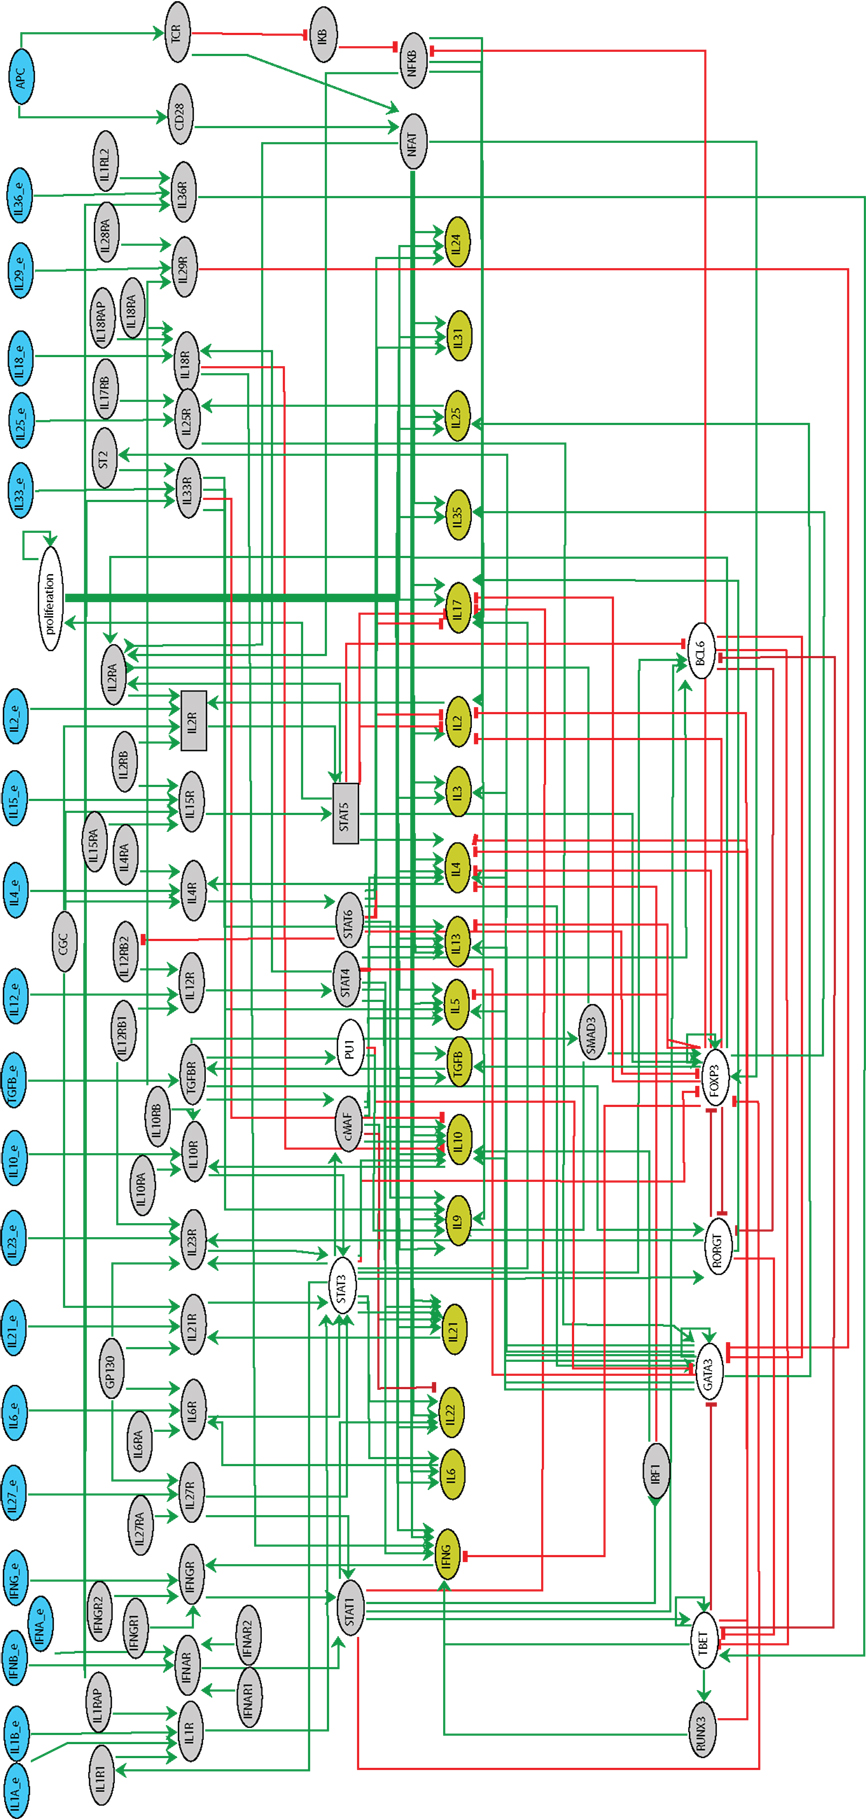
\includegraphics[scale=0.18,angle=-90]{images/th_differentiation.jpg}
\end{center}
\begin{center}
 {\tiny \color{darkgreen} [\citeatfb]}
\end{center}
\end{frame}



%mettre le tableau
\begin{frame}[c]
 \frametitle{Results of identification of bifurcations}
 

%mettre le tableau
\begin{table}[bt]
\renewcommand{\arraystretch}{1.3}

\centering
%table of result
\scalebox{0.8}{
\setlength{\tabcolsep}{2mm}
\begin{tabular}{|c|c||c|r||c|r||c|r|}
\hline
\multirow{2}{*}{Automata Network} 
& \multirow{2}{*}{Goal}
& \multicolumn{2}{c||}{M-C (NuSMV)}
& \multicolumn{2}{c||}{with \iIIIa}
& \multicolumn{2}{c|}{with \iIIIb}
\\
\cline{3-8}
&&$\card{t_b}$&Time&$\card{t_b}$&Time&$\card{t_b}$&Time
\\\hline

Lambda phage &  $\mathrm{CI}_2$ & $10$ & $0.1s$ & $6$ & $0.1s$ & $0$ & $0.2s$ 	
\\
$\card\anN=4\quad\card\anT=11$ &$\mathrm{Cro}_2$ & $3$ & $0.1s$ & $3$ & $0.1s$ & $2$ & $0.3s$ 	
\\ \hline 

EGF/TNF       & $\mathrm{NFkB}_0$ & $5$ & $0.2s$ & $4$ & $0.1s$ & $2$ & $0.1s$ 
\\

$\card\anN=28\quad\card\anT=55$ & $\mathrm{IKB}_1$ & $5$ & $0.2s$ & $3$ & $0.1s$ & $2$ & $0.1s$ 

\\ \hline

Th\_th17 & $\mathrm{RORGT}_1$ & $18$ & $48s$ & $9$ & $23s$ & $8$ & $26s$  
\\
$\card\anN=101\quad\card\anT=381$ & $\mathrm{BCL6}_1$ &$7$ & $26s$ &$5$ & $23s$ & $4$ & $24s$ 

\\ \hline

Th\_HTG & $\mathrm{BCL6}_1$ & \multicolumn{2}{c||}{\multirow{2}{*}{out-of-time}} & \multicolumn{2}{c||}{\multirow{2}{*}{out-of-time}} & $6$ & $61s$ 

\\

$\card\anN=101\quad\card\anT=381$ & $\mathrm{GATA3}_1$ &  \multicolumn{2}{c||}{} &\multicolumn{2}{c||}{}  & $7$ & $34s$ 

\\ \hline



\end{tabular}
}
\end{table}
\begin{center} Implemented in ASP (Answer Set Programming) and solve with clingo 4.5.4.\end{center}
\end{frame}

\begin{frame}
%mettre cette slide un peu avant la conclusion
\frametitle{Automata Network modelling of Biological Networks}
\textbf{Transition-centered specification}
\begin{itemize}
\item ...in opposition to function-centered of Boolean/Thomas networks
\item explicit context/ \tval{causality of state changes}
\item closely related to (safe) Petri nets
\item step semantics (purely async, purely sync, mixed)
\end{itemize}
\textbf{Modelling}
\begin{itemize}
\item any Boolean/Thomas networks can be encoded;
\item in case of logical rules uncertainty: \tval{model the union} of Boolean/Thomas networks (over-approximation of behaviours)
%\item encoding of \tval{SBGN Process Description} models
\end{itemize}
\end{frame}



%%%%%%%%    la conclusion
%\section{Conclusions \& Perspectives}
%% Performances et conclusion
\begin{frame}[c]
  \frametitle{Conclusions}

%mots clés: large scale
%bien expliquer les résultats obtenus
% \textbf{Summary}


\textbf{Hybrid approach for modelling an RSTC network}
  \begin{itemize}
   \item Formalizing biological knowledge: Translation of motifs in AN.
   %\item Automatic generation of Automata networks model
   \item Inference and integration of temporal parameters
   \item Qualitative and quantitative refinement of dynamics 
  \end{itemize}

\textbf{Static analysis of quantitative property (Probability/delay)}
\begin{itemize}
 \item 
  $$
\left\{
    \begin{array}{lcl}
        \mbox{QS (Quotient set)} &\\  %rajouter un signe entre les deux
        \mbox{+} & \Longrightarrow \mbox{\tval{formal approximation of}} \\
        \mbox{AI (Abstract interpretation)} & \mbox{\tval{\ \ \quantitative properties}}
    \end{array}
\right.
$$ 
 \item Estimation of a lower bound of probability and delay of reachability property 
 \item Good theoretical complexity
\end{itemize}



\textbf{Identification of Bifurcations}
 \begin{itemize}
\item 
$$
\left\{
    \begin{array}{lcl}
        \mbox{AI (Artificial inteligence)} &\\  %rajouter un signe entre les deux
        \mbox{+} & \Longrightarrow \mbox{\tval{formal approximation of bifurcations}} \\
        \mbox{AI (Abstract interpretation)} &
    \end{array}
\right.
$$ 
   \item Tractable on large networks (compared to model-checking)
   \item Under-approximation: some bifurcations are not returned.
   %\item Application on \tval{Phage lambda, EGF/TNF, Th\_differentiation} 
  \end{itemize}
\medskip

\end{frame}

%rajouter les slides du titre




%\begin{frame}
 \frametitle{Perspectives}
 
 \textbf{Stochastic simulation \& statistic analysis}
 \begin{itemize}
  \item Statistic analysis which take into account time.
  \item Use association rules to identify interesting relations between components.
 \end{itemize}

 
 \textbf{Static analysis of probability}
 \begin{itemize}
  \item Implementation (in progress...) of a static analyzer for properties in  CCSL Logic
  \item Static analysis of long run behaviors (steady state)
  \item Static analysis of parametric models
 \end{itemize}

 
 \textbf{Identification of Bifurcations}
 \begin{itemize}
%parler d'améliorer les conditions initiales
  \item Over-approximation of bifurcations
  %\item Frame the number of attractors
  \item Use bifurcations for the analysis of probability 
  \item Applications for \tval{predicting targets for cellular reprogramming.}
  
 \end{itemize}
%\medskip

 
 
%  \begin{block}{Formal verification of quantitative properties and key process (in progress)}
%   \begin{itemize}
%    \item Static analysis of quantitative properties of reachability in Asynchronous automata networks
%    \item Logical verification and key processes detection
%    \item Experimental validation of in silico hypotesis
%    %\item Integrate de likelihood in the parameters estimation procedure.
%   \end{itemize}
% 
%  \end{block}
%  
%  \begin{block}{Association rules and traces in automata networks}
%   \begin{itemize}
%    \item Association rules for discovering interesting relations between local states. 
%    \item Experimental validation of in silico hypotesis
%   \end{itemize}
% 
%  \end{block}
 
\end{frame}




%slides en français

%%%%%%%%     introduction
\section{Introduction}
% Diapo d'intro
\begin{frame}
\frametitle{Contexte}

%introduire le développement des méthodes informatiques pour les systèmes complexes
%en particulier les systèmes biologiques dans le but de comprendre, modifier et 
%éventuellement contrôler le vivant. Ce qui implique donc de pouvoir 
% (1) Modéliser  (2) analyser (3) vérifier les comportements souhaités ou non.



%faire le lien entre modélisation, analyse et vérification des systèmes biologiques

%definition analyse: Étude minutieuse, précise faite pour dégager les éléments qui constituent un ensemble, pour l'expliquer, l'éclairer 

%definition vérification: vérifier si le modèle d'un système (souvent informatique ou électronique) satisfait une propriété. Par exemple, on souhaite vérifier qu'un programme ne se bloque pas, qu'une variable n'est jamais nulle, etc. 
\begin{tikzpicture}
 
 \uncover<2->{\node[auto] (sc) at (0,2) {Systèmes complexes};}
 \node[auto] (sb) at (0,1.5) {Systèmes \tval{bio}logiques};
 \only<1>{\node[esdef] (defsb) at (4,-5) {\begin{tabular}{c} Un système biologique est un ensemble d'organes/composants interagissant au \\ sein d'un organisme dans la réalisation d'une fonction biologique commune. \end{tabular}};}
\only<2>{\node[esdef] (defsc) at (4,-5) {\begin{tabular}{c} Systèmes complexes sont des réseaux des composants inter-agissants entre eux, \\ généralement de façon non déterministe. \end{tabular}};}

 
 
 \uncover<3->{\node[auto] (mi) at (7,1.5) {Méthodes \tval{informatiques}};
 
 \node[auto] (plus) at (3.5,1.5) {+};}
 
 \only<3>{\node[esdef] (defmi) at (4,-5) {\begin{tabular}{c} Méthodes informatiques: traitement automatique de l'information. \\\end{tabular}};}

 
 \uncover<4->{\node[es] (modeliser) at (0,-2) {Modéliser};}
 
 \only<4>{\node[esdef] (defmod) at (4,-5) {\begin{tabular}{c} Un modèle est une représentation simplifiée d'un système.\\ \end{tabular}};}

 
 \uncover<5->{\node[es] (analyser) at (3,-1) {Analyser};}
 
 \only<5>{\node[esdef] (defana) at (4,-5) {\begin{tabular}{c} Une analyse est une  étude minutieuse, précise faite pour comprendre\\ un système (modèle), pour l'expliquer, l'éclairer. \end{tabular}};}

 
 \uncover<6->{\node[es] (verifier) at (3,-3) {Vérifier};}

 \only<6>{\node[esdef] (defverif) at (4,-5) {\begin{tabular}{c} Une vérification (formelle) est le fait de prouver (de façon formelle)\\ la présence ou non d'une propriété dans un système. \end{tabular}};}

 
 
\uncover<7->{ 
\node (d1) at (4,-2) {};
\node (d2) at (6.5,-2) {};
 
 \draw[->,line width=6pt, color=lightgray] (d1) -- (d2) ;
 
 \node[auto] (butmodel) at (8,-2) {$
 \left\{
    \begin{array}{llll}
        Comprendre \\
        Prédire \\
        Modifier \\
        Contrôler
    \end{array}
\right.
$};
\begin{pgfonlayer}{background}
\draw[draw=blue!50, rounded corners=2mm, fill = white!20]
(-1.1, -3.4) rectangle (4.1, -0.5);
\end{pgfonlayer}
 }
 
 
\only<8>{\node[esdef] (but) at (4,-5) {\begin{tabular}{c}But: \tval{Développer les méthodes efficaces (complexité de calcul)}\\ \tval{pour l'analyse des grands modèles.}\end{tabular}};}
 \node[auto] (bp) at (4,-5.5) {};
%node[above=10pt,midway]{\textcolor{black}{\textbf{Algebraic Modelling}}} 
\end{tikzpicture}





\end{frame}




\begin{frame}[c]
  \frametitle{Contexte}
%rajouter le titre (version courte) dans toute les slides
\begin{center}
  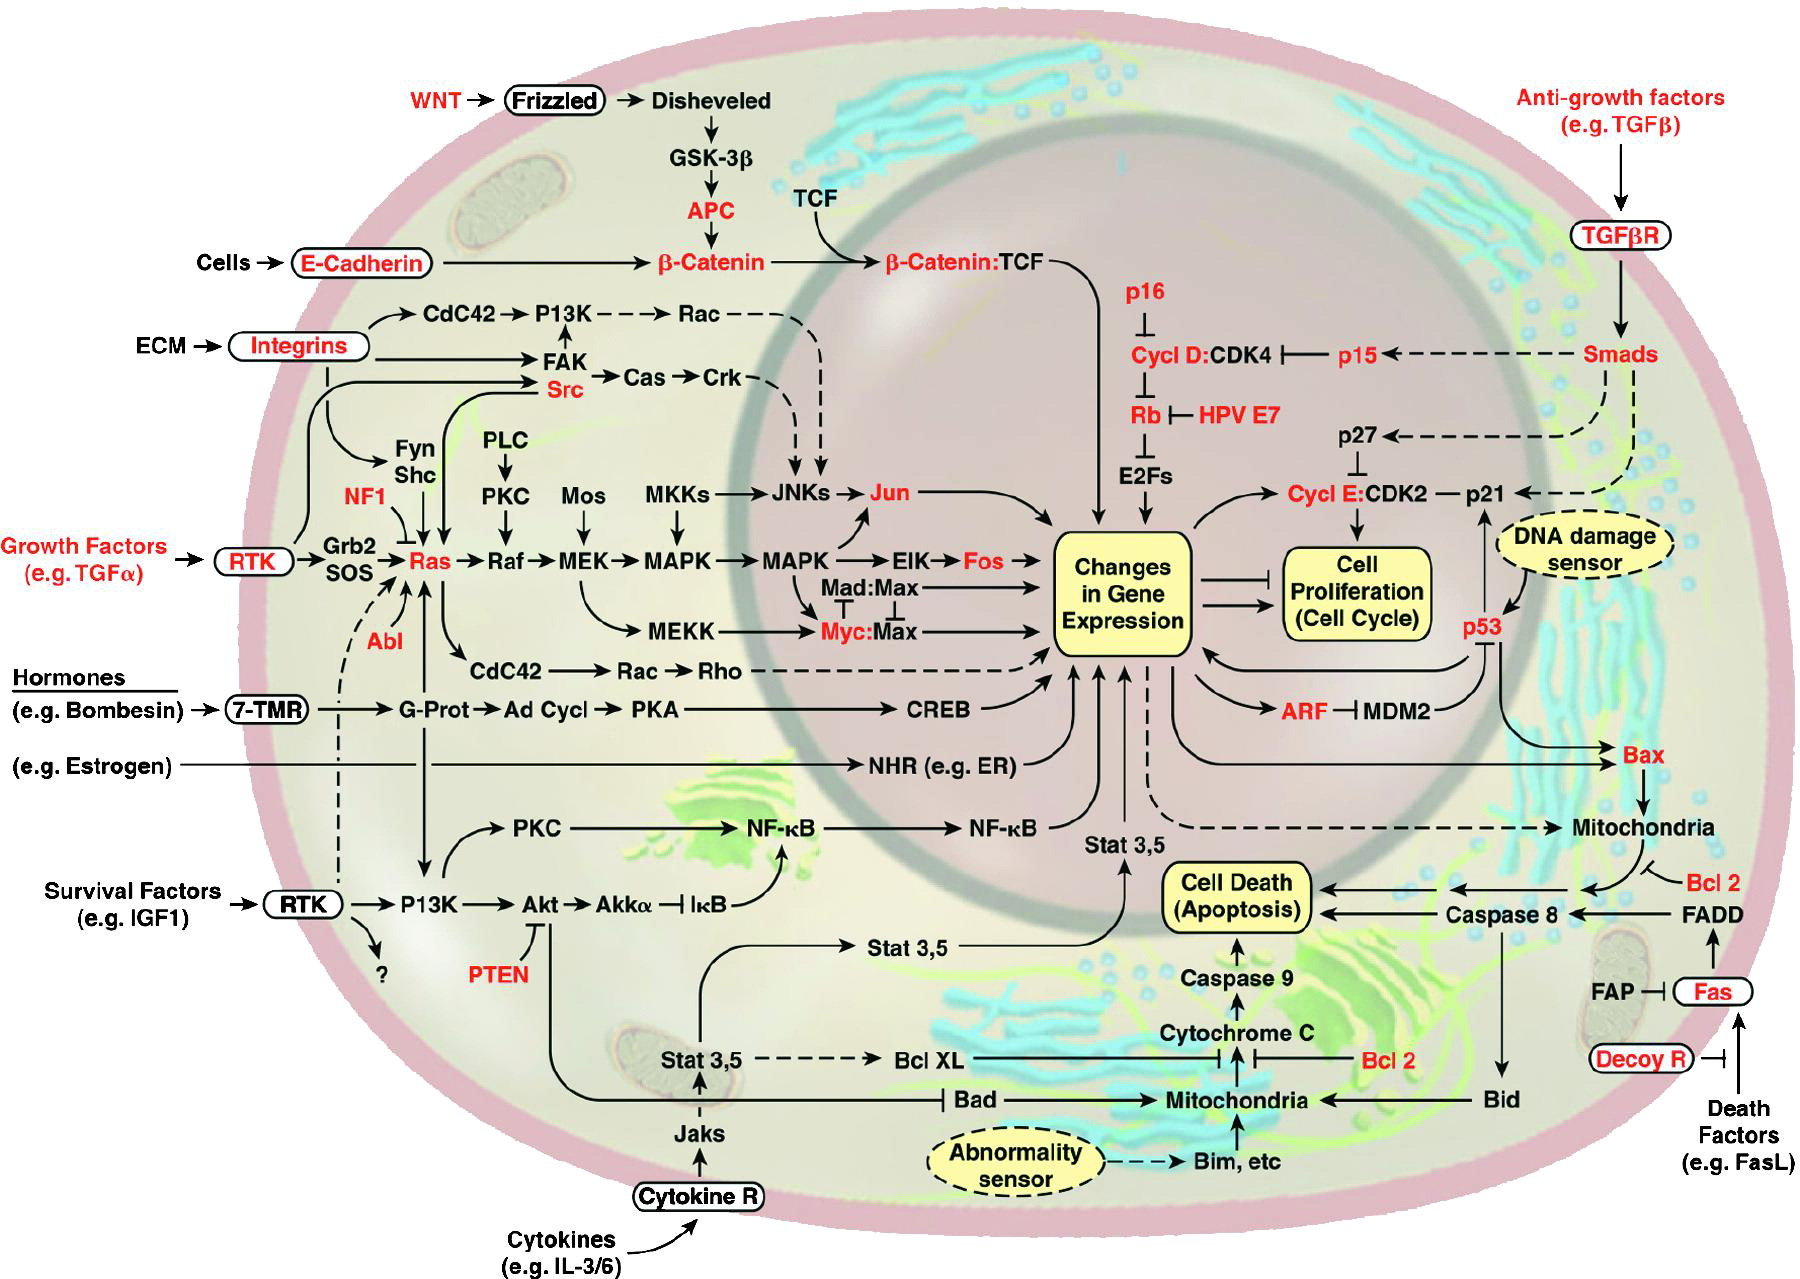
\includegraphics[scale=0.12]{images/cellule-description.jpeg}
\end{center}
\begin{center}
{\tiny \color{darkgreen}[\citelui]}
\end{center}

%\tcite{Wikipédia}

\begin{itemize}
%\item Cellular processes are driven by networks of biological interactions.
\item Processus cellulaire $\Longrightarrow$ des réseaux de régulation biologique (RRB).
\item N{\oe}uds (les composants biologiques), les arcs (les interactions).
%\item Proposer une modélisation formelle et une analyse des RRB.
%\item Formal modelling and analysis of Biological Regulatory Network.
%\item Static analysis of qualitative and quantitative properties.
\end{itemize}

%Cellular processes are driven by networks of biological reactions. Cells rely on the tight coordination of these pathways to achieve proper functioning.
%With the help of signaling pathway, a cell senses changes in its environnement or internal state. This information is then passed on via cascades of biochemical 
%reactions to the appropriate mechanisms which respond by modifying the metabolic and transcriptiona activities. this in turn modifies the behavior of the cell.

%Consequently, the dynamics of biopathways play a crucial role in determinig cellular functions.

%Examples: circadian rhythm, the apoptosis pathway inducing programmed cell death, cell differentiation.

%\textcolor{couleurtheme}{$\Rightarrow$} \fbox{\tval{\large The need of comprehension of biological systems}} \textcolor{couleurtheme}{$\Leftarrow$}


%\textcolor{couleurtheme}{$\Rightarrow$} \fbox{\tval{\large Allow efficient translation from Process Hitting to BRN}} \textcolor{couleurtheme}{$\Leftarrow$}

\end{frame}



\section{\'Etat de l'art}
% \begin{frame}
% \frametitle{Modélisation des réseaux de régulation biologique}
% 
% \begin{itemize}
%  \item 
%  \item 
% \end{itemize}
%\end{frame}

\begin{frame}
\frametitle{Modélisation discrètes}

\begin{itemize}
 \item Chaque composant possède un nombre fini de \tval{niveaux qualitatifs} (\{0,1,2,...\}).
 \item Fonctions donnant le \tval{niveau suivant l'état des régulateurs.}
\end{itemize}
\bigskip
\begin{tikzpicture}
 \node[scale=1] (brn) at (0,5) {\begin{tikzpicture}[grn]
      \path[use as bounding box] (-0.3,-0.75) rectangle (4,.75);
      \node[inner sep=0] (b) at (2,0) {b};
      \node[inner sep=0] (a) at (0,0) {a};
            
      \node[elabel, below=-.8em of a] {$0..2$};
      \node[elabel, below=-.8em of b] {$0..1$};
     
      
      \path[->]
        (a) edge[loop above] node[elabel, above=-5pt] {$+2$}
        (a) edge[bend right] node[elabel, below=-5pt] {$+1$} (b)
        (b) edge[bend right] node[elabel, above=-5pt] {$-1$} (a);
    \end{tikzpicture}};
 
\node (plus) at (-1,3.5) {\textbf{+}};
    
\node (ft) at (-1,3) {Fonction de transition};

\node[auto] (sg) at (6,4) {
\begin{tikzpicture}[node distance=1.5cm]
  \node (s01) {$\RRBetat{a_0,b_1}$};
  \node[right of=s01] (s11) {$\RRBetat{a_1,b_1}$};
  \node[right of=s11] (s21) {$\RRBetat{a_2,b_1}$};
  \node[below of=s01, node distance=1cm] (s00) {$\RRBetat{a_0,b_0}$};
  \node[right of=s00] (s10) {$\RRBetat{a_1,b_0}$};
  \node[right of=s10] (s20) {$\RRBetat{a_2,b_0}$};
  \path[->]
    (s01) edge (s00)
    (s00) edge (s10)
    (s10) edge (s11)
    (s11) edge (s01)
    (s10) edge (s20)
    (s20) edge (s21)
  ;
\end{tikzpicture}};
%\node[scale=0.6] (sg) at (2,1) {
\begin{tikzpicture}[line join=bevel,font=\LARGE]
%%
  \node (6) at (405.0bp,18.0bp) [reach,nd4] {$\langle a_2,b_1,c_0\rangle$};
  \node (2) at (405.0bp,90.0bp) [reach,nd3] {$\langle a_2,b_0,c_0\rangle$};
  \node (1) at (570.0bp,90.0bp) [reach,nd1] {$\langle a_1,b_0,c_0\rangle$};
  \node (0) at (469.0bp,162.0bp) [reach,nd0] {$s_0 = \langle a_0,b_0,c_0\rangle$};
  \node (4) at (469.0bp,234.0bp) [reach,nd5] {$\langle a_0,b_1,c_0\rangle$};
 
 
  \draw [->,arc3] (0) ..controls (445.65bp,135.46bp) and (435.95bp,124.86bp)  .. (2);
  \draw [->,arc5] (0) ..controls (475.71bp,188.03bp) and (475.94bp,197.36bp)  .. (4);
  \draw [->,arc4] (2) ..controls (405.0bp,63.983bp) and (405.0bp,54.712bp)  .. (6);
  \draw [->,arc1] (0) ..controls (499.93bp,134.79bp) and (517.41bp,122.58bp)  .. (1);
  \draw [->,arc2] (1) ..controls (539.0bp,117.26bp) and (521.52bp,129.47bp)  .. (0);
  \draw [->,arc5] (4) ..controls (462.3bp,208.35bp) and (462.06bp,199.03bp)  .. (0);
 
%
\end{tikzpicture}

};
\path 
(2,4) edge[->,line width=6pt, color=lightgray] (sg)
;
\end{tikzpicture}

\begin{center}
 {\small \color{darkgreen} [\citekauffman]}\\
 {\small \color{darkgreen} [\citethomas]}
\end{center}

\end{frame}


\begin{frame}
\frametitle{Modélisation hybride}
\framesubtitle{\'Etats discrets et transitions caractéristiques hybrides}

\tval{Introduction de l'aléatoire et du temps pour les transitions}\\
\medskip
\textbf{Modèles stochastiques} \\
Variables aléatoires généralement exponentielles. 
\begin{itemize}
 \item $\pi$-calcul stochastique. 
 \item Réseaux de Petri stochastiques.
\end{itemize}
% \begin{center}
% {\small \color{darkgreen} [\citestocha]}\\
%  
% \end{center}


\bigskip

\textbf{Modèles temporisés}
\begin{itemize}
 \item Automates temporisés / hybrides.
 \item Réseaux de Petri temporisés.
\end{itemize}

\medskip

\textbf{Frappes de processus}.
% \begin{center}
% {\small \color{darkgreen} [\citetemp]}\\
% 
% \end{center}


%nécessité d'estimer les paramètre à partir des données 

\end{frame}



 
 %parler des données
 
 \section{Contributions}
 \begin{frame}[c]
 \frametitle{Contributions}
 
 \begin{tikzpicture}[auto]
 
 \draw[thick, ->] (-3.5,0)--node[near end,above,rotate=90] {\scriptsize Niveau d'abstraction des dynamiques}(-3.5,8);
 
 \node[debutfin,align=center] (niv1) at (-2,7) {\begin{tikzpicture}[auto,scale=0.5] 
                                                 \path[use as bounding box] (-0.7,-0.3) rectangle (2.5,2);

                                                              \node[qgre,scale=0.5] (a) at (0,2) {a};
                                                              \node[mod,scale=0.5] (i) at (1,1) {i};
                                                              \node[qgre,scale=0.5] (b) at (0,0) {b};
                                                              \node[qgre,scale=0.5] (c) at (2,1) {c};
                                                              \path
                                                                (a) edge[inh,scale=0.1] (i)
                                                                (b) edge[act,scale=0.1] (i)
                                                                (i) edge[st,scale=0.1]  (c);
                                                              
                                                 \end{tikzpicture}};
                                                 
 \node[debutfin,align=center] (niv2) at (-2,4) {\begin{tikzpicture}[auto,scale=0.5] 
                                                 \path[use as bounding box] (-0.7,-0.3) rectangle (2.5,2);

                                                              \node[qgre,scale=0.5] (a) at (0,2) {a};
                                                              \node[mod,scale=0.5] (i) at (1,1) {i};
                                                              \node[qgre,scale=0.5] (b) at (0,0) {b};
                                                              \node[qgre,scale=0.5] (c) at (2,1) {c};
                                                              \path
                                                                (a) edge[inh,scale=0.1] (i)
                                                                (b) edge[act,scale=0.1] (i)
                                                                (i) edge[st,scale=0.1]  (c);
                                                                
                                                  \node[grandplus] (plus) at (1.2,0.2) {$+$};
                                                  \node[grandplus] (plus) at (2,0) {$K$};
                                                              
                                                 \end{tikzpicture}};
                                                
 \node[debutfin,align=center] (niv3) at (-2,1) {\begin{tikzpicture}[auto,scale=0.5] 
                                                 \path[use as bounding box] (-0.7,-0.3) rectangle (2.5,2);

                                                              \node[qgre,scale=0.5] (a) at (0,2) {a};
                                                              \node[mod,scale=0.5] (i) at (1,1) {i};
                                                              \node[qgre,scale=0.5] (b) at (0,0) {b};
                                                              \node[qgre,scale=0.5] (c) at (2,1) {c};
                                                              \path
                                                                (a) edge[inh,scale=0.1] (i)
                                                                (b) edge[act,scale=0.1] (i)
                                                                (i) edge[st,scale=0.1]  (c);
                                                                
                                                  \node[grandplus] (plus) at (1,0) {$+$};
                                                  \node[grandplus] (plus) at (2,0.5) {$K$};
                                                  \node[scale=0.5] (clock) at (2,-0.25) {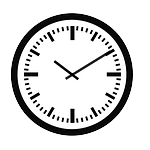
\includegraphics[scale=0.22]{figs/clock.png}};
                                                              
                                                 \end{tikzpicture}};
                                                 

 
 %\node[grandplus] (plus) at (2,0) {$+$};
 
 \uncover<2->{
 
 \draw[thick, ->] (7.8,8)--node[near end,below,rotate=90] {\scriptsize Précision des propriétés}(7.8,0); %ligne de la précision des propriétés 
 
 
 
 
 % liste des propriétés
 %general properties
 \node[instruct,align=center] (gp) at (5.8,7) {\begin{tabular}{c}
                                            {\scriptsize Propriétés générales: bornes} \\ 
                                            {\scriptsize sur le nbr d'attracteurs;}\\ {\scriptsize fonctionnalités,...}
                                           \end{tabular}};
 
 %fixed points
 \node[instruct,align=center] (fp) at (6.7,5.6) {\begin{tabular}{c}
                                                 {\scriptsize \'Etats stables}
                                                 \end{tabular}};
                                           
 %reachabilities
 \node[instruct,align=center] (reach) at (6.7,4) {\begin{tabular}{c} {\scriptsize Accessibilité} \\ {\scriptsize Bifurcations} \\ {\scriptsize (CTL)} \end{tabular}};
 \node[instruct,align=center] (qreach) at (6.7,1) {\begin{tabular}{c} {\scriptsize Accessibilité} \\ {\scriptsize quantitative} \\{\scriptsize (CCSL)} \end{tabular}};
 }
 
 %%CTL
% \node[instruct,align=center] (CTL) at (6.15,3.2) {{ \scriptsize CTL (logique temporelle)}};
 
 %CSL
 %\node[instruct,align=center] (CSL) at (5.8,0.7) {\begin{tabular}{c} {\scriptsize CCSL (logique, conccurrente }\\
 %                                                 {\scriptsize  continue, stochastique)}
 %                                               \end{tabular}};
 
 %process hitting
 
 \uncover<3-4>{
 
% \begin{pgfonlayer}{background}
 \draw[->,color=gray!40,bend right,line width=4pt,round] (niv3)--node[near center,below] {\scriptsize Analyse dynamique quantitative}(qreach);
 
 \draw[->,color=gray!40,bend right,line width=0.5pt] (niv1)--node[near center,below] {\scriptsize Analyse statique } (gp);
 
 \draw[->,color=gray!40,bend right,line width=0.6pt,round] (niv2)--node[near center,above] {\scriptsize Analyse statique }(fp);
 
 \draw[->,color=gray!40,bend right,line width=2pt,round] (niv2)--node[near center,below] {\scriptsize Analyse dynamique }(reach);
% \end{pgfonlayer}
 
 }
 
 
 
%  \uncover<3->{
%  
% % \begin{pgfonlayer}{background}
%  \draw[->,color=gray!20,bend right,line width=4pt,round] (niv3)--node[near center,below] {\scriptsize }(qreach);
%  
%  \draw[->,color=gray!20,bend right,line width=0.5pt] (niv1)-- (gp);
%  
%   \draw[->,color=gray!40,bend right,line width=0.6pt,round] (niv2)--node[near center,below] {\scriptsize }(fp);
%  
%  \draw[->,color=gray!20,bend right,line width=2pt,round] (niv2)--node[near center,below] {\scriptsize }(reach);
% % \end{pgfonlayer}
%  
%  }
 
 \uncover<4->{
  
 %ajout de la notion de chronométrie
 \draw[gray!80,loosely dashed] (-4,2.5) -- node[very near start,below] {\scriptsize Chronométrie}node[very near start,above] {\scriptsize Chronologie}(8,2.5);

 
 }
 
%  \uncover<5->{
%  \node[es,align=center] (ph) at (2,4.5) {\begin{tabular}{c}
%                                            {\scriptsize \textbf{Réseaux} }\\ 
%                                            {\scriptsize \textbf{d'Automates}}
%                                            \end{tabular}};
%  \node[instruct,align=center] (pint) at (2,3) {\scriptsize PINT};
%  \draw[->,dashed] (ph)--(pint);
%  }
%  
%  
%  %les relations
%  \uncover<6->{
%  \draw[suite] (niv1)--(ph);
%  \draw[suite] (niv2)--(ph);
%  \draw[suite,color=blue] (niv3)--node[near center,above,bend right,rotate=45] {\scriptsize Modélisation}(ph);
%  
%  %\draw[->] (CTL)--(reach);
%  %\draw[->] (CSL)--(qreach);
%  
%  %\draw[suite] (ph)--(gp);
%  \draw[suite,line width=0.5pt] (ph)--node[near center,above,rotate=18] {\scriptsize analyse statique}(fp);
%  
%  \draw[suite,blue] (ph)--node[near center,above,blue,rotate=-5] {\scriptsize analyse statique}(reach);
% 
%  \draw[suite,color=blue] (ph)--node[near center,above,rotate=-35] {\scriptsize analyse statique}(qreach);
% 
%  
%  
%  \draw[suite,blue,round]     (pint) --node[near center,above,bend right,rotate=90] {\scriptsize Simulation}(2,1.5)-- node[near center,above,bend right] {\scriptsize Analyse} (niv3);
%  }

  
 \end{tikzpicture}

 
\end{frame}

\begin{frame}[c]
 \frametitle{Contributions}
 
 \begin{tikzpicture}[auto]
 
 \draw[thick, ->] (-3.5,0)--node[near end,above,rotate=90] {\scriptsize Niveau d'abstraction des dynamiques}(-3.5,8);
 
 \node[debutfin,align=center] (niv1) at (-2,7) {\begin{tikzpicture}[auto,scale=0.5] 
                                                 \path[use as bounding box] (-0.7,-0.3) rectangle (2.5,2);

                                                              \node[qgre,scale=0.5] (a) at (0,2) {a};
                                                              \node[mod,scale=0.5] (i) at (1,1) {i};
                                                              \node[qgre,scale=0.5] (b) at (0,0) {b};
                                                              \node[qgre,scale=0.5] (c) at (2,1) {c};
                                                              \path
                                                                (a) edge[inh,scale=0.1] (i)
                                                                (b) edge[act,scale=0.1] (i)
                                                                (i) edge[st,scale=0.1]  (c);
                                                              
                                                 \end{tikzpicture}};
                                                 
 \node[debutfin,align=center] (niv2) at (-2,4) {\begin{tikzpicture}[auto,scale=0.5] 
                                                 \path[use as bounding box] (-0.7,-0.3) rectangle (2.5,2);

                                                              \node[qgre,scale=0.5] (a) at (0,2) {a};
                                                              \node[mod,scale=0.5] (i) at (1,1) {i};
                                                              \node[qgre,scale=0.5] (b) at (0,0) {b};
                                                              \node[qgre,scale=0.5] (c) at (2,1) {c};
                                                              \path
                                                                (a) edge[inh,scale=0.1] (i)
                                                                (b) edge[act,scale=0.1] (i)
                                                                (i) edge[st,scale=0.1]  (c);
                                                                
                                                  \node[grandplus] (plus) at (1.2,0.2) {$+$};
                                                  \node[grandplus] (plus) at (2,0) {$K$};
                                                              
                                                 \end{tikzpicture}};
                                                
 \node[debutfin,align=center] (niv3) at (-2,1) {\begin{tikzpicture}[auto,scale=0.5] 
                                                 \path[use as bounding box] (-0.7,-0.3) rectangle (2.5,2);

                                                              \node[qgre,scale=0.5] (a) at (0,2) {a};
                                                              \node[mod,scale=0.5] (i) at (1,1) {i};
                                                              \node[qgre,scale=0.5] (b) at (0,0) {b};
                                                              \node[qgre,scale=0.5] (c) at (2,1) {c};
                                                              \path
                                                                (a) edge[inh,scale=0.1] (i)
                                                                (b) edge[act,scale=0.1] (i)
                                                                (i) edge[st,scale=0.1]  (c);
                                                                
                                                  \node[grandplus] (plus) at (1,0) {$+$};
                                                  \node[grandplus] (plus) at (2,0.5) {$K$};
                                                  \node[scale=0.5] (clock) at (2,-0.25) {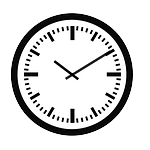
\includegraphics[scale=0.22]{figs/clock.png}};
                                                              
                                                 \end{tikzpicture}};
                                                 

 
 %\node[grandplus] (plus) at (2,0) {$+$};
 

 
 \draw[thick, ->] (7.8,8)--node[near end,below,rotate=90] {\scriptsize Précision des propriétés}(7.8,0); %ligne de la précision des propriétés 
 
 
 
 
 % liste des propriétés
 %general properties
 \node[instruct,align=center] (gp) at (5.8,7) {\begin{tabular}{c}
                                            {\scriptsize Propriétés générales: bornes} \\ 
                                            {\scriptsize sur le nbr d'attracteurs;}\\ {\scriptsize fonctionnalités,...}
                                           \end{tabular}};
 
 %fixed points
 \node[instruct,align=center] (fp) at (6.7,5.6) {\begin{tabular}{c}
                                                 {\scriptsize \'Etats stables}
                                                 \end{tabular}};
                                           
 %reachabilities
 \node[instruct,align=center] (reach) at (6.7,4) {\begin{tabular}{c} {\scriptsize Accessibilité} \\ {\scriptsize Bifurcations} \\ {\scriptsize (CTL)} \end{tabular}};
 \node[instruct,align=center] (qreach) at (6.7,1) {\begin{tabular}{c} {\scriptsize Accessibilité} \\ {\scriptsize quantitative} \\{\scriptsize (CCSL)} \end{tabular}};
 
 
 %process hitting
 

 
 
 
 \uncover<1->{
 
% \begin{pgfonlayer}{background}
 \draw[->,color=gray!20,bend right,line width=4pt,round] (niv3)--node[near center,below] {\scriptsize }(qreach);
 
 \draw[->,color=gray!20,bend right,line width=0.5pt] (niv1)-- (gp);
 
  \draw[->,color=gray!40,bend right,line width=0.6pt,round] (niv2)--node[near center,below] {\scriptsize }(fp);
 
 \draw[->,color=gray!20,bend right,line width=2pt,round] (niv2)--node[near center,below] {\scriptsize }(reach);
% \end{pgfonlayer}
 
   
 %ajout de la notion de chronométrie
 \draw[gray!80,loosely dashed] (-4,2.5) -- node[very near start,below] {\scriptsize Chronométrie}node[very near start,above] {\scriptsize Chronologie}(8,2.5);

 
 }
 
%  \uncover<4->{
%  \node[es,align=center] (ph) at (2,4.5) {\begin{tabular}{c}
%                                            {\scriptsize \textbf{Réseaux} }\\ 
%                                            {\scriptsize \textbf{d'Automates}}
%                                            \end{tabular}};
%  \node[instruct,align=center] (pint) at (2,3) {\scriptsize PINT};
%  \draw[->,dashed] (ph)--(pint);
%  }
%  
%  
%  %les relations
%  \uncover<5->{
%  \draw[suite] (niv1)--(ph);
%  \draw[suite] (niv2)--(ph);
%  \draw[suite,color=blue] (niv3)--node[near center,above,bend right,rotate=45] {\scriptsize Modélisation}(ph);
%  
%  %\draw[->] (CTL)--(reach);
%  %\draw[->] (CSL)--(qreach);
%  
%  %\draw[suite] (ph)--(gp);
%  \draw[suite,line width=0.5pt] (ph)--node[near center,above,rotate=18] {\scriptsize analyse statique}(fp);
%  
%  \draw[suite,blue] (ph)--node[near center,above,blue,rotate=-5] {\scriptsize analyse statique}(reach);
% 
%  \draw[suite,color=blue] (ph)--node[near center,above,rotate=-35] {\scriptsize analyse statique}(qreach);
% 
%  
%  
%  \draw[suite,blue,round]     (pint) --node[near center,above,bend right,rotate=90] {\scriptsize Simulation}(2,1.5)-- node[near center,above,bend right] {\scriptsize Analyse} (niv3);
%  }

  
 \end{tikzpicture}

 
\end{frame}

\begin{frame}[c]
 \frametitle{Contributions}
 
 \begin{tikzpicture}[auto]
 
 \draw[thick, ->] (-3.5,0)--node[near end,above,rotate=90] {\scriptsize Niveau d'abstraction des dynamiques}(-3.5,8);
 
 \node[debutfin,align=center] (niv1) at (-2,7) {\begin{tikzpicture}[auto,scale=0.5] 
                                                 \path[use as bounding box] (-0.7,-0.3) rectangle (2.5,2);

                                                              \node[qgre,scale=0.5] (a) at (0,2) {a};
                                                              \node[mod,scale=0.5] (i) at (1,1) {i};
                                                              \node[qgre,scale=0.5] (b) at (0,0) {b};
                                                              \node[qgre,scale=0.5] (c) at (2,1) {c};
                                                              \path
                                                                (a) edge[inh,scale=0.1] (i)
                                                                (b) edge[act,scale=0.1] (i)
                                                                (i) edge[st,scale=0.1]  (c);
                                                              
                                                 \end{tikzpicture}};
                                                 
 \node[debutfin,align=center] (niv2) at (-2,4) {\begin{tikzpicture}[auto,scale=0.5] 
                                                 \path[use as bounding box] (-0.7,-0.3) rectangle (2.5,2);

                                                              \node[qgre,scale=0.5] (a) at (0,2) {a};
                                                              \node[mod,scale=0.5] (i) at (1,1) {i};
                                                              \node[qgre,scale=0.5] (b) at (0,0) {b};
                                                              \node[qgre,scale=0.5] (c) at (2,1) {c};
                                                              \path
                                                                (a) edge[inh,scale=0.1] (i)
                                                                (b) edge[act,scale=0.1] (i)
                                                                (i) edge[st,scale=0.1]  (c);
                                                                
                                                  \node[grandplus] (plus) at (1.2,0.2) {$+$};
                                                  \node[grandplus] (plus) at (2,0) {$K$};
                                                              
                                                 \end{tikzpicture}};
                                                
 \node[debutfin,align=center] (niv3) at (-2,1) {\begin{tikzpicture}[auto,scale=0.5] 
                                                 \path[use as bounding box] (-0.7,-0.3) rectangle (2.5,2);

                                                              \node[qgre,scale=0.5] (a) at (0,2) {a};
                                                              \node[mod,scale=0.5] (i) at (1,1) {i};
                                                              \node[qgre,scale=0.5] (b) at (0,0) {b};
                                                              \node[qgre,scale=0.5] (c) at (2,1) {c};
                                                              \path
                                                                (a) edge[inh,scale=0.1] (i)
                                                                (b) edge[act,scale=0.1] (i)
                                                                (i) edge[st,scale=0.1]  (c);
                                                                
                                                  \node[grandplus] (plus) at (1,0) {$+$};
                                                  \node[grandplus] (plus) at (2,0.5) {$K$};
                                                  \node[scale=0.5] (clock) at (2,-0.25) {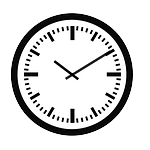
\includegraphics[scale=0.22]{figs/clock.png}};
                                                              
                                                 \end{tikzpicture}};
                                                 

 
 %\node[grandplus] (plus) at (2,0) {$+$};
 

 
 \draw[thick, ->] (7.8,8)--node[near end,below,rotate=90] {\scriptsize Précision des propriétés}(7.8,0); %ligne de la précision des propriétés 
 
 
 
 
 % liste des propriétés
 %general properties
 \node[instruct,align=center] (gp) at (5.8,7) {\begin{tabular}{c}
                                            {\scriptsize Propriétés générales: bornes} \\ 
                                            {\scriptsize sur le nbr d'attracteurs;}\\ {\scriptsize fonctionnalités,...}
                                           \end{tabular}};
 
 %fixed points
 \node[instruct,align=center] (fp) at (6.7,5.6) {\begin{tabular}{c}
                                                 {\scriptsize \'Etats stables}
                                                 \end{tabular}};
                                           
 %reachabilities
 \node[instruct,align=center] (reach) at (6.7,4) {\begin{tabular}{c} {\scriptsize Bifurcations} \\ {\scriptsize Accessibilité} \\ {\scriptsize (CTL)} \end{tabular}};
 \node[instruct,align=center] (qreach) at (6.7,1) {\begin{tabular}{c} {\scriptsize Accessibilité} \\ {\scriptsize quantitative} \\{\scriptsize (CCSL)} \end{tabular}};
 
 
 %process hitting
 

 
 
 
 \uncover<1->{
 
% \begin{pgfonlayer}{background}
 \draw[->,color=gray!10,bend right,line width=4pt,round] (niv3)--node[near center,below] {\scriptsize }(qreach);
 
 \draw[->,color=gray!10,bend right,line width=0.5pt] (niv1)-- (gp);
 
  \draw[->,color=gray!10,bend right,line width=0.6pt,round] (niv2)--node[near center,below] {\scriptsize }(fp);
 
 \draw[->,color=gray!10,bend right,line width=2pt,round] (niv2)--node[near center,below] {\scriptsize }(reach);
% \end{pgfonlayer}
 
   
 %ajout de la notion de chronométrie
 \draw[gray!80,loosely dashed] (-4,2.5) -- node[very near start,below] {\scriptsize Chronométrie}node[very near start,above] {\scriptsize Chronologie}node[very near end,below] {\scriptsize Quantitative}node[very near end,above] {\scriptsize Qualitative}(8,2.5);

 
 }
 
 \uncover<1->{
 \node[es,align=center] (ph) at (2,4.5) {\begin{tabular}{c}
                                           {\scriptsize \textbf{Réseaux} }\\ 
                                           {\scriptsize \textbf{d'Automates}}
                                           \end{tabular}};
 \node[instruct,align=center] (pint) at (2,3) {\scriptsize PINT};
 \draw[->,dashed] (ph)--(pint);
 }
 
 
 %les relations
 \uncover<2->{
 \draw[suite,color=gray] (niv1)--(ph);
 \draw[suite,color=gray] (niv2)--(ph);
  \draw[suite,color=gray,line width=0.5pt] (ph)--node[near center,above,rotate=18] {\scriptsize Analyse statique}(fp);
 \draw[suite,color=blue] (niv3)--node[near center,above,bend right,rotate=45] {\scriptsize Modélisation}node[inner,below]{1.A}(ph);
 }
\uncover<3->{
 
 \draw[suite,blue,round]     (pint) --node[near center,above,bend right,rotate=90] {\scriptsize Simulation}node[inner,right]{1.B}(2,1.5)-- node[near center,above,bend right] {\scriptsize Analyse} (niv3);
 }

 \uncover<4->{

 \draw[suite,color=blue] (ph)--node[near center,above,rotate=-35] {\scriptsize Analyse statique}node[inner,below]{2}(qreach);

 }
 
 \uncover<5->{
  
 \draw[suite,blue] (ph)--node[near center,above,blue,rotate=-5] {\scriptsize Analyse statique}node[inner,below]{3}(reach);

 }
  
 \end{tikzpicture}
 
\end{frame}


\begin{frame}[c]
 \frametitle{Contributions}
 
 \begin{tikzpicture}[auto]
 
 \draw[thick, ->] (-3.5,0)--node[near end,above,rotate=90] {\scriptsize Niveau d'abstraction des dynamiques}(-3.5,8);
 
 \node[debutfin,align=center] (niv1) at (-2,7) {\begin{tikzpicture}[auto,scale=0.5] 
                                                 \path[use as bounding box] (-0.7,-0.3) rectangle (2.5,2);

                                                              \node[qgre,scale=0.5] (a) at (0,2) {a};
                                                              \node[mod,scale=0.5] (i) at (1,1) {i};
                                                              \node[qgre,scale=0.5] (b) at (0,0) {b};
                                                              \node[qgre,scale=0.5] (c) at (2,1) {c};
                                                              \path
                                                                (a) edge[inh,scale=0.1] (i)
                                                                (b) edge[act,scale=0.1] (i)
                                                                (i) edge[st,scale=0.1]  (c);
                                                              
                                                 \end{tikzpicture}};
                                                 
 \node[debutfin,align=center] (niv2) at (-2,4) {\begin{tikzpicture}[auto,scale=0.5] 
                                                 \path[use as bounding box] (-0.7,-0.3) rectangle (2.5,2);

                                                              \node[qgre,scale=0.5] (a) at (0,2) {a};
                                                              \node[mod,scale=0.5] (i) at (1,1) {i};
                                                              \node[qgre,scale=0.5] (b) at (0,0) {b};
                                                              \node[qgre,scale=0.5] (c) at (2,1) {c};
                                                              \path
                                                                (a) edge[inh,scale=0.1] (i)
                                                                (b) edge[act,scale=0.1] (i)
                                                                (i) edge[st,scale=0.1]  (c);
                                                                
                                                  \node[grandplus] (plus) at (1.2,0.2) {$+$};
                                                  \node[grandplus] (plus) at (2,0) {$K$};
                                                              
                                                 \end{tikzpicture}};
                                                
 \node[debutfin,align=center] (niv3) at (-2,1) {\begin{tikzpicture}[auto,scale=0.5] 
                                                 \path[use as bounding box] (-0.7,-0.3) rectangle (2.5,2);

                                                              \node[qgre,scale=0.5] (a) at (0,2) {a};
                                                              \node[mod,scale=0.5] (i) at (1,1) {i};
                                                              \node[qgre,scale=0.5] (b) at (0,0) {b};
                                                              \node[qgre,scale=0.5] (c) at (2,1) {c};
                                                              \path
                                                                (a) edge[inh,scale=0.1] (i)
                                                                (b) edge[act,scale=0.1] (i)
                                                                (i) edge[st,scale=0.1]  (c);
                                                                
                                                  \node[grandplus] (plus) at (1,0) {$+$};
                                                  \node[grandplus] (plus) at (2,0.5) {$K$};
                                                  \node[scale=0.5] (clock) at (2,-0.25) {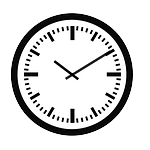
\includegraphics[scale=0.22]{figs/clock.png}};
                                                              
                                                 \end{tikzpicture}};
                                                 

 
 %\node[grandplus] (plus) at (2,0) {$+$};
 

 
 \draw[thick, ->] (7.8,8)--node[near end,below,rotate=90] {\scriptsize Précision des propriétés}(7.8,0); %ligne de la précision des propriétés 
 
 
 
 
 % liste des propriétés
 %general properties
 \node[instruct,align=center] (gp) at (5.8,7) {\begin{tabular}{c}
                                            {\scriptsize \textbf{\underline{Propriétés générales:}} bornes} \\ 
                                            {\scriptsize sur le nbr d'attracteurs;}\\ {\scriptsize fonctionnalités,...}
                                           \end{tabular}};
 
 %fixed points
 \node[instruct,align=center] (fp) at (6.7,5.6) {\begin{tabular}{c}
                                                 {\scriptsize \'Etats stables}
                                                 \end{tabular}};
                                           
 %reachabilities
 \node[instruct,align=center] (reach) at (6.7,4) {\begin{tabular}{c} {\scriptsize Bifurcations} \\ {\scriptsize Accessibilité} \\ {\scriptsize (CTL)} \end{tabular}};
 \node[instruct,align=center] (qreach) at (6.7,1) {\begin{tabular}{c} {\scriptsize Accessibilité} \\ {\scriptsize quantitative} \\{\scriptsize (CCSL)} \end{tabular}};
 
 
 %process hitting
 

 
 
 
 \uncover<1->{
 
% \begin{pgfonlayer}{background}
 \draw[->,color=gray!10,bend right,line width=4pt,round] (niv3)--node[near center,below] {\scriptsize }(qreach);
 
 \draw[->,color=gray!10,bend right,line width=0.5pt] (niv1)-- (gp);
 
  \draw[->,color=gray!10,bend right,line width=0.6pt,round] (niv2)--node[near center,below] {\scriptsize }(fp);
 
 \draw[->,color=gray!10,bend right,line width=2pt,round] (niv2)--node[near center,below] {\scriptsize }(reach);
% \end{pgfonlayer}
 
   
 %ajout de la notion de chronométrie
 \draw[gray!80,loosely dashed] (-4,2.5) -- node[very near start,below] {\scriptsize Chronométrie}node[very near start,above] {\scriptsize Chronologie}node[very near end,below] {\scriptsize Quantitative}node[very near end,above] {\scriptsize Qualitative}(8,2.5);

 
 }
 
 \uncover<1->{
 \node[es,align=center] (ph) at (2,4.5) {\begin{tabular}{c}
                                           {\scriptsize \textbf{Réseaux} }\\ 
                                           {\scriptsize \textbf{d'automates}}
                                           \end{tabular}};
 \node[instruct,align=center] (pint) at (2,3) {\scriptsize PINT};
 \draw[->,dashed] (ph)--(pint);
 }
 
 
 %les relations
 \uncover<1->{
 \draw[suite,color=gray] (niv1)--(ph);
 \draw[suite,color=gray] (niv2)--(ph);
  \draw[suite,line width=0.5pt,color=gray] (ph)--node[near center,above,rotate=18] {\scriptsize analyse statique}(fp);
 \draw[suite,color=blue!60] (niv3)--node[near center,above,bend right,rotate=45] {\scriptsize Modélisation}node[inner,below]{1.A}(ph);
 \draw[suite,blue!60,round]     (pint) --node[near center,above,bend right,rotate=90] {\scriptsize Simulation}node[inner,right]{1.B}(2,1.5)-- node[near center,above,bend right] {\scriptsize Analyse} (niv3);
 \draw[suite,color=blue!60] (ph)--node[near center,above,rotate=-35] {\scriptsize analyse statique}node[inner,below]{2}(qreach);
  \draw[suite,blue!60] (ph)--node[near center,above,blue!60,rotate=-5] {\scriptsize analyse statique}node[inner,below]{3}(reach);
 }
 

  
 \end{tikzpicture}

 
\end{frame}



% 
%rappeler l'approche ici 
 \subsection{Les réseaux d'automates}
 % Définition du Process Hitting + sortes coopératives

\begin{frame}
  \frametitle{Réseaux d'automates (AN)}
  %\framesubtitle{\tcite{Paulev\'e et al. 2012}}


\begin{columns}
\begin{column}{0.6\textwidth}
% 1 : Sortes
\only<1>{
\tikzstyle{process}=[circle,minimum size=15pt,font=\footnotesize,inner sep=1pt]
\tikzstyle{tick label}=[color=white, font=\footnotesize]
\tikzstyle{tick}=[transparent]
\tikzstyle{hit}=[transparent]
\tikzstyle{selfhit}=[transparent, min distance=30pt,curve to]
\tikzstyle{bounce}=[transparent]
\tikzstyle{hlhit}=[transparent]
\tikzstyle{local transitions}=[transparent]
\begin{center}\scalebox{\scaleex}{
\begin{tikzpicture}
\exandef
\end{tikzpicture}
}\end{center}
}

% 2 : Processus
\only<2>{
\tikzstyle{process}=[circle,draw,minimum size=15pt,font=\footnotesize,inner sep=1pt]
\tikzstyle{tick label}=[font=\footnotesize]
\tikzstyle{tick}=[densely dotted]
\tikzstyle{hit}=[transparent]
\tikzstyle{selfhit}=[transparent, min distance=30pt,curve to]
\tikzstyle{bounce}=[transparent]
\tikzstyle{hlhit}=[transparent]
\tikzstyle{local transitions}=[transparent]
\begin{center}\scalebox{\scaleex}{
\begin{tikzpicture}
\exandef
\end{tikzpicture}
}\end{center}
}

% 3 : États
\only<3>{
\tikzstyle{hit}=[transparent]
\tikzstyle{selfhit}=[transparent, min distance=30pt,curve to]
\tikzstyle{bounce}=[transparent]
\tikzstyle{hlhit}=[transparent]
\tikzstyle{local transitions}=[transparent]
\begin{center}\scalebox{\scaleex}{
\begin{tikzpicture}
\exandef

\TState{3}{a_0,b_0,c_0}
\end{tikzpicture}
}\end{center}
}

% 4 : Actions
\only<4->{
\tikzstyle{tick}=[densely dotted]
\tikzstyle{hit}=[->,>=angle 45]
\tikzstyle{selfhit}=[min distance=30pt,curve to]
\tikzstyle{bounce}=[densely dotted,>=stealth',->]
\tikzstyle{hlhit}=[very thick]
\begin{center}\scalebox{\scaleex}{
\begin{tikzpicture}
\exandef
\TState{4}{a_0,b_0,c_0}
\TState{5}{a_1,b_0,c_0}
\TState{6}{a_0,b_0,c_0}
\TState{7}{a_2,b_0,c_0}
\TState{8}{a_2,b_1,c_0}
\end{tikzpicture}
}\end{center}
}
\end{column}

\begin{column}{0.4\textwidth}
\begin{figure}[p]
\centering

\scalebox{0.4}{
\only<4>{
\tikzstyle{arc0}=[transparent]
\tikzstyle{nd0}=[]
\tikzstyle{arc1}=[transparent]
\tikzstyle{nd1}=[transparent]
\tikzstyle{arc2}=[transparent]
\tikzstyle{nd2}=[transparent]
\tikzstyle{arc3}=[transparent]
\tikzstyle{nd3}=[transparent]
\tikzstyle{arc4}=[transparent]
\tikzstyle{nd4}=[transparent]
\tikzstyle{arc5}=[transparent]
\tikzstyle{nd5}=[transparent]

\begin{tikzpicture}[line join=bevel,font=\LARGE]
%%
  \node (6) at (405.0bp,18.0bp) [reach,nd4] {$\langle a_2,b_1,c_0\rangle$};
  \node (2) at (405.0bp,90.0bp) [reach,nd3] {$\langle a_2,b_0,c_0\rangle$};
  \node (1) at (570.0bp,90.0bp) [reach,nd1] {$\langle a_1,b_0,c_0\rangle$};
  \node (0) at (469.0bp,162.0bp) [reach,nd0] {$s_0 = \langle a_0,b_0,c_0\rangle$};
  \node (4) at (469.0bp,234.0bp) [reach,nd5] {$\langle a_0,b_1,c_0\rangle$};
 
 
  \draw [->,arc3] (0) ..controls (445.65bp,135.46bp) and (435.95bp,124.86bp)  .. (2);
  \draw [->,arc5] (0) ..controls (475.71bp,188.03bp) and (475.94bp,197.36bp)  .. (4);
  \draw [->,arc4] (2) ..controls (405.0bp,63.983bp) and (405.0bp,54.712bp)  .. (6);
  \draw [->,arc1] (0) ..controls (499.93bp,134.79bp) and (517.41bp,122.58bp)  .. (1);
  \draw [->,arc2] (1) ..controls (539.0bp,117.26bp) and (521.52bp,129.47bp)  .. (0);
  \draw [->,arc5] (4) ..controls (462.3bp,208.35bp) and (462.06bp,199.03bp)  .. (0);
 
%
\end{tikzpicture}


}
\only<5>{
\tikzstyle{arc0}=[->]
\tikzstyle{nd0}=[]
\tikzstyle{arc1}=[->]
\tikzstyle{nd1}=[]
\tikzstyle{arc2}=[transparent]
\tikzstyle{nd2}=[transparent]
\tikzstyle{arc3}=[transparent]
\tikzstyle{nd3}=[transparent]
\tikzstyle{arc4}=[transparent]
\tikzstyle{nd4}=[transparent]
\tikzstyle{arc5}=[transparent]
\tikzstyle{nd5}=[transparent]

\begin{tikzpicture}[line join=bevel,font=\LARGE]
%%
  \node (6) at (405.0bp,18.0bp) [reach,nd4] {$\langle a_2,b_1,c_0\rangle$};
  \node (2) at (405.0bp,90.0bp) [reach,nd3] {$\langle a_2,b_0,c_0\rangle$};
  \node (1) at (570.0bp,90.0bp) [reach,nd1] {$\langle a_1,b_0,c_0\rangle$};
  \node (0) at (469.0bp,162.0bp) [reach,nd0] {$s_0 = \langle a_0,b_0,c_0\rangle$};
  \node (4) at (469.0bp,234.0bp) [reach,nd5] {$\langle a_0,b_1,c_0\rangle$};
 
 
  \draw [->,arc3] (0) ..controls (445.65bp,135.46bp) and (435.95bp,124.86bp)  .. (2);
  \draw [->,arc5] (0) ..controls (475.71bp,188.03bp) and (475.94bp,197.36bp)  .. (4);
  \draw [->,arc4] (2) ..controls (405.0bp,63.983bp) and (405.0bp,54.712bp)  .. (6);
  \draw [->,arc1] (0) ..controls (499.93bp,134.79bp) and (517.41bp,122.58bp)  .. (1);
  \draw [->,arc2] (1) ..controls (539.0bp,117.26bp) and (521.52bp,129.47bp)  .. (0);
  \draw [->,arc5] (4) ..controls (462.3bp,208.35bp) and (462.06bp,199.03bp)  .. (0);
 
%
\end{tikzpicture}


}
\only<6>{
\tikzstyle{arc0}=[->]
\tikzstyle{nd0}=[]
\tikzstyle{arc1}=[->]
\tikzstyle{nd1}=[]
\tikzstyle{arc2}=[->]
\tikzstyle{nd2}=[]
\tikzstyle{arc3}=[transparent]
\tikzstyle{nd3}=[transparent]
\tikzstyle{arc4}=[transparent]
\tikzstyle{nd4}=[transparent]
\tikzstyle{arc5}=[transparent]
\tikzstyle{nd5}=[transparent]

\begin{tikzpicture}[line join=bevel,font=\LARGE]
%%
  \node (6) at (405.0bp,18.0bp) [reach,nd4] {$\langle a_2,b_1,c_0\rangle$};
  \node (2) at (405.0bp,90.0bp) [reach,nd3] {$\langle a_2,b_0,c_0\rangle$};
  \node (1) at (570.0bp,90.0bp) [reach,nd1] {$\langle a_1,b_0,c_0\rangle$};
  \node (0) at (469.0bp,162.0bp) [reach,nd0] {$s_0 = \langle a_0,b_0,c_0\rangle$};
  \node (4) at (469.0bp,234.0bp) [reach,nd5] {$\langle a_0,b_1,c_0\rangle$};
 
 
  \draw [->,arc3] (0) ..controls (445.65bp,135.46bp) and (435.95bp,124.86bp)  .. (2);
  \draw [->,arc5] (0) ..controls (475.71bp,188.03bp) and (475.94bp,197.36bp)  .. (4);
  \draw [->,arc4] (2) ..controls (405.0bp,63.983bp) and (405.0bp,54.712bp)  .. (6);
  \draw [->,arc1] (0) ..controls (499.93bp,134.79bp) and (517.41bp,122.58bp)  .. (1);
  \draw [->,arc2] (1) ..controls (539.0bp,117.26bp) and (521.52bp,129.47bp)  .. (0);
  \draw [->,arc5] (4) ..controls (462.3bp,208.35bp) and (462.06bp,199.03bp)  .. (0);
 
%
\end{tikzpicture}


}
\only<7>{
\tikzstyle{arc0}=[->]
\tikzstyle{nd0}=[]
\tikzstyle{arc1}=[->]
\tikzstyle{nd1}=[]
\tikzstyle{arc2}=[->]
\tikzstyle{nd2}=[]
\tikzstyle{arc3}=[->]
\tikzstyle{nd3}=[]
\tikzstyle{arc4}=[transparent]
\tikzstyle{nd4}=[transparent]
\tikzstyle{arc5}=[transparent]
\tikzstyle{nd5}=[transparent]

\begin{tikzpicture}[line join=bevel,font=\LARGE]
%%
  \node (6) at (405.0bp,18.0bp) [reach,nd4] {$\langle a_2,b_1,c_0\rangle$};
  \node (2) at (405.0bp,90.0bp) [reach,nd3] {$\langle a_2,b_0,c_0\rangle$};
  \node (1) at (570.0bp,90.0bp) [reach,nd1] {$\langle a_1,b_0,c_0\rangle$};
  \node (0) at (469.0bp,162.0bp) [reach,nd0] {$s_0 = \langle a_0,b_0,c_0\rangle$};
  \node (4) at (469.0bp,234.0bp) [reach,nd5] {$\langle a_0,b_1,c_0\rangle$};
 
 
  \draw [->,arc3] (0) ..controls (445.65bp,135.46bp) and (435.95bp,124.86bp)  .. (2);
  \draw [->,arc5] (0) ..controls (475.71bp,188.03bp) and (475.94bp,197.36bp)  .. (4);
  \draw [->,arc4] (2) ..controls (405.0bp,63.983bp) and (405.0bp,54.712bp)  .. (6);
  \draw [->,arc1] (0) ..controls (499.93bp,134.79bp) and (517.41bp,122.58bp)  .. (1);
  \draw [->,arc2] (1) ..controls (539.0bp,117.26bp) and (521.52bp,129.47bp)  .. (0);
  \draw [->,arc5] (4) ..controls (462.3bp,208.35bp) and (462.06bp,199.03bp)  .. (0);
 
%
\end{tikzpicture}


}
\only<8>{
\tikzstyle{arc0}=[->]
\tikzstyle{nd0}=[]
\tikzstyle{arc1}=[->]
\tikzstyle{nd1}=[]
\tikzstyle{arc2}=[->]
\tikzstyle{nd2}=[]
\tikzstyle{arc3}=[->]
\tikzstyle{nd3}=[]
\tikzstyle{arc4}=[->]
\tikzstyle{nd4}=[]
\tikzstyle{arc5}=[transparent]
\tikzstyle{nd5}=[transparent]

\begin{tikzpicture}[line join=bevel,font=\LARGE]
%%
  \node (6) at (405.0bp,18.0bp) [reach,nd4] {$\langle a_2,b_1,c_0\rangle$};
  \node (2) at (405.0bp,90.0bp) [reach,nd3] {$\langle a_2,b_0,c_0\rangle$};
  \node (1) at (570.0bp,90.0bp) [reach,nd1] {$\langle a_1,b_0,c_0\rangle$};
  \node (0) at (469.0bp,162.0bp) [reach,nd0] {$s_0 = \langle a_0,b_0,c_0\rangle$};
  \node (4) at (469.0bp,234.0bp) [reach,nd5] {$\langle a_0,b_1,c_0\rangle$};
 
 
  \draw [->,arc3] (0) ..controls (445.65bp,135.46bp) and (435.95bp,124.86bp)  .. (2);
  \draw [->,arc5] (0) ..controls (475.71bp,188.03bp) and (475.94bp,197.36bp)  .. (4);
  \draw [->,arc4] (2) ..controls (405.0bp,63.983bp) and (405.0bp,54.712bp)  .. (6);
  \draw [->,arc1] (0) ..controls (499.93bp,134.79bp) and (517.41bp,122.58bp)  .. (1);
  \draw [->,arc2] (1) ..controls (539.0bp,117.26bp) and (521.52bp,129.47bp)  .. (0);
  \draw [->,arc5] (4) ..controls (462.3bp,208.35bp) and (462.06bp,199.03bp)  .. (0);
 
%
\end{tikzpicture}


}
\only<9>{
\tikzstyle{arc0}=[->]
\tikzstyle{nd0}=[]
\tikzstyle{arc1}=[->]
\tikzstyle{nd1}=[]
\tikzstyle{arc2}=[->]
\tikzstyle{nd2}=[]
\tikzstyle{arc3}=[->]
\tikzstyle{nd3}=[]
\tikzstyle{arc4}=[->]
\tikzstyle{nd4}=[]
\tikzstyle{arc5}=[->]
\tikzstyle{nd5}=[]

\begin{tikzpicture}[line join=bevel,font=\LARGE]
%%
  \node (6) at (405.0bp,18.0bp) [reach,nd4] {$\langle a_2,b_1,c_0\rangle$};
  \node (2) at (405.0bp,90.0bp) [reach,nd3] {$\langle a_2,b_0,c_0\rangle$};
  \node (1) at (570.0bp,90.0bp) [reach,nd1] {$\langle a_1,b_0,c_0\rangle$};
  \node (0) at (469.0bp,162.0bp) [reach,nd0] {$s_0 = \langle a_0,b_0,c_0\rangle$};
  \node (4) at (469.0bp,234.0bp) [reach,nd5] {$\langle a_0,b_1,c_0\rangle$};
 
 
  \draw [->,arc3] (0) ..controls (445.65bp,135.46bp) and (435.95bp,124.86bp)  .. (2);
  \draw [->,arc5] (0) ..controls (475.71bp,188.03bp) and (475.94bp,197.36bp)  .. (4);
  \draw [->,arc4] (2) ..controls (405.0bp,63.983bp) and (405.0bp,54.712bp)  .. (6);
  \draw [->,arc1] (0) ..controls (499.93bp,134.79bp) and (517.41bp,122.58bp)  .. (1);
  \draw [->,arc2] (1) ..controls (539.0bp,117.26bp) and (521.52bp,129.47bp)  .. (0);
  \draw [->,arc5] (4) ..controls (462.3bp,208.35bp) and (462.06bp,199.03bp)  .. (0);
 
%
\end{tikzpicture}


}
}

\end{figure}

\end{column}
\end{columns}
%\medskip

\begin{liste}
  \item \tval{Automate}: composants \qex{$a$, $b$, $c$}.
\pause[2]
  \item \tval{\'Etats locaux}: niveaux d'expression \qex{$c_0$, $c_1$, $c_2$}.
\pause[3]
  \item \tval{\'Etats}: l'ensemble des états locaux actifs%
  \only<3-4>{\qex{$\PHetat{a_0, b_0, c_0}$}}%
  \only<5>{\qex{$\PHetat{a_1, b_0, c_0}$}}%
  \only<6>{\qex{$\PHetat{a_0, b_0, c_0}$}}%
  \only<7>{\qex{$\PHetat{a_2, b_0, c_0}$}}%
  \only<8>{\qex{$\PHetat{a_2, b_1, c_0}$}}
\pause[4]
  \item \tval{Transitions}: dynamique  \qex{\only<5>{\underline}{$t_1 = \trans{a_0}{a_1}{b_0}$}, \only<6>{\underline}{$t_2 = \trans{a_1}{a_0}{}$}, \only<7>{\underline}{$t_3 = \trans{a_0}{a_2}{b_0,c_0}$}, \only<8>{\underline}{$t_4 = \trans{b_0}{b_1}{}$}}
\end{liste}
%une seule transition à la fois
%on peut avoir un choix il faut bien expliquer ça.
\end{frame}


 % Stochasticité

\begin{frame}
  \frametitle{Paramètres temporels et stochastiques}
  %\framesubtitle{\tcite{Paulev\'e et al. 2010}}
Idée: Calibrage temporel réglable avec un paramètre stochastique.
\begin{center}
 {\small \color{darkgreen} [\citepmrtcsb]}
\end{center}


%Paramétrage d'une transition
\begin{itemize}
  \item \tval{Taux $r$}  \& \tval{facteur d'absorption de stochasticité $sa$}.
  %\item Durée de l'action $\approx$ somme de $sa$ avec un taux $r.sa$.
  \item Durée moyenne: $r^{-1}$; variance: $r^{-2}sa^{-1}$ (distribution d'Erlang).
  \item Paramètres: soit $(r,sa)$, ou l'intervalle de tir $[d;D]$.
%   \begin{fleches}
%     \item Tests by simulation
%   \end{fleches}
\end{itemize}

%\begin{columns}
%\begin{column}{0.5\textwidth}

\only<1->{
\scalebox{0.9}{
\begin{tikzpicture}[plot,xscale=0.35,yscale=1]
\draw[axe] (0,0) -- (15.5,0) node[right] {$t$};
\draw[axe] (0,0) -- (0,1);
\draw[ticks] (0,0) node[below] {$0$};
\draw[mean] (4,0) -- (4,0.9) node[right]{$\frac{1}{r}$};
\draw[dashed] (0.10127,0) -- (0.10127,0.9) node[right] {$d$} (14.75552,0) --
(14.75552,0.9) node[left] {$D$};
\pgfplothandlerlineto
\pgfplotxyfile{plots/BioAtlanSTIC-0409/erlang-0.25-1.table}
\pgfusepath{stroke}
\draw[interval] (0.10127,0) -- (14.75552,0);
\end{tikzpicture}
}

\scalebox{0.9}{
\begin{tikzpicture}[plot,xscale=0.35,yscale=1]
\draw[axe] (0,0) -- (15.5,0) node[right] {$t$};
\draw[axe] (0,0) -- (0,1);
\draw[ticks] (0,0) node[below] {$0$};
\draw[mean] (4,0) -- (4,0.9) node[right]{$\frac{1}{r}$};
\draw[dashed] (1.29879,0) -- (1.29879,0.9) node[right] {$d$} (8.19327,0) --
(8.19327,0.9) node[left] {$D$};
\pgfplothandlerlineto
\pgfplotxyfile{plots/BioAtlanSTIC-0409/erlang-0.25-5.table}
\pgfusepath{stroke}
\draw[interval] (1.29879,0) -- (8.19327,0);
\end{tikzpicture}
}

\scalebox{0.9}{
\begin{tikzpicture}[plot,xscale=0.35,yscale=1]
\draw[axe] (0,0) -- (15.5,0) node[right] {$t$};
\draw[axe] (0,0) -- (0,1);
\draw[ticks] (0,0) node[below] {$0$};
\draw[mean] (4,0) -- (4,0.9) node[right]{$\frac{1}{r}$};
\draw[dashed] (2.96888,0) -- (2.96888,0.9) node[left] {$d$} (5.18245,0) --
(5.18245,0.9) node[right] {$D$};
\pgfplothandlerlineto
\pgfplotxyfile{plots/BioAtlanSTIC-0409/erlang-0.25-50.table}
\pgfusepath{stroke}
\draw[interval] (2.96888,0) -- (5.18245,0);
\end{tikzpicture}
}

~~\textcolor{lightred}{\rule{17mm}{4.5pt}} ~ temps d'une action
}

%\end{column}
\end{frame}

 \subsection{Les réseaux d'automates stochastiques}
 % Définition du Process Hitting + sortes coopératives

%san presentation
\begin{comment}
\begin{frame}
\frametitle{Biological networks modelling}
\begin{tikzpicture}
\node (brn) at (0,5) {\begin{tikzpicture}[auto,scale=0.9] 
                                                 \path[use as bounding box] (-0.7,-0.3) rectangle (2.5,2);

                                                              \node[qgre,scale=0.8] (a) at (0,2) {a};
                                                              \node[mod,scale=0.8] (i) at (1,1) {i};
                                                              \node[qgre,scale=0.8] (b) at (0,0) {b};
                                                              \node[qgre,scale=0.8] (c) at (2,1) {c};
                                                              \path
                                                                (a) edge[inh,scale=0.1] (i)
                                                                (b) edge[act,scale=0.1] (i)
                                                                (i) edge[st,scale=0.1]  (c);
                                                              
                                                 \end{tikzpicture}};
\node[scale=0.6] (an) at (7,5) {\begin{tikzpicture}
\exandef
\end{tikzpicture}};
\node[scale=0.6] (sg) at (2,1) {
\begin{tikzpicture}[line join=bevel,font=\LARGE]
%%
  \node (6) at (405.0bp,18.0bp) [reach,nd4] {$\langle a_2,b_1,c_0\rangle$};
  \node (2) at (405.0bp,90.0bp) [reach,nd3] {$\langle a_2,b_0,c_0\rangle$};
  \node (1) at (570.0bp,90.0bp) [reach,nd1] {$\langle a_1,b_0,c_0\rangle$};
  \node (0) at (469.0bp,162.0bp) [reach,nd0] {$s_0 = \langle a_0,b_0,c_0\rangle$};
  \node (4) at (469.0bp,234.0bp) [reach,nd5] {$\langle a_0,b_1,c_0\rangle$};
 
 
  \draw [->,arc3] (0) ..controls (445.65bp,135.46bp) and (435.95bp,124.86bp)  .. (2);
  \draw [->,arc5] (0) ..controls (475.71bp,188.03bp) and (475.94bp,197.36bp)  .. (4);
  \draw [->,arc4] (2) ..controls (405.0bp,63.983bp) and (405.0bp,54.712bp)  .. (6);
  \draw [->,arc1] (0) ..controls (499.93bp,134.79bp) and (517.41bp,122.58bp)  .. (1);
  \draw [->,arc2] (1) ..controls (539.0bp,117.26bp) and (521.52bp,129.47bp)  .. (0);
  \draw [->,arc5] (4) ..controls (462.3bp,208.35bp) and (462.06bp,199.03bp)  .. (0);
 
%
\end{tikzpicture}

};
\path 
(brn) edge[->,line width=8pt, color=lightgray] (an)
(an) edge[->,line width=8pt, color=lightgray,bend left] (sg)
;

\end{tikzpicture}
\end{frame}


\begin{frame}
  \frametitle{Réseaux d'automates stochastiques}
  
\begin{columns}
\begin{column}{0.6\textwidth}

% Automate sans les rates
\only<1->{
\tikzstyle{tick}=[densely dotted]
\tikzstyle{hit}=[->,>=angle 45]
\tikzstyle{selfhit}=[min distance=30pt,curve to]
\tikzstyle{bounce}=[densely dotted,>=stealth',->]
\tikzstyle{hlhit}=[very thick]
\begin{center}\scalebox{\scaleex}{
\begin{tikzpicture}
\exandef
\end{tikzpicture}
}\end{center}
}
\end{column}

\begin{column}{0.4\textwidth}
\begin{figure}[p]
\centering

\scalebox{0.4}{

\only<1->{
\tikzstyle{arc0}=[->]
\tikzstyle{nd0}=[]
\tikzstyle{arc1}=[->]
\tikzstyle{nd1}=[]
\tikzstyle{arc2}=[->]
\tikzstyle{nd2}=[]
\tikzstyle{arc3}=[->]
\tikzstyle{nd3}=[]
\tikzstyle{arc4}=[->]
\tikzstyle{nd4}=[]
\tikzstyle{arc5}=[->]
\tikzstyle{nd5}=[]

\begin{tikzpicture}[line join=bevel,font=\LARGE]
%%
  \node (6) at (405.0bp,18.0bp) [reach,nd4] {$\langle a_2,b_1,c_0\rangle$};
  \node (2) at (405.0bp,90.0bp) [reach,nd3] {$\langle a_2,b_0,c_0\rangle$};
  \node (1) at (570.0bp,90.0bp) [reach,nd1] {$\langle a_1,b_0,c_0\rangle$};
  \node (0) at (469.0bp,162.0bp) [reach,nd0] {$s_0 = \langle a_0,b_0,c_0\rangle$};
  \node (4) at (469.0bp,234.0bp) [reach,nd5] {$\langle a_0,b_1,c_0\rangle$};
 
 
  \draw [->,arc3] (0) ..controls (445.65bp,135.46bp) and (435.95bp,124.86bp)  .. (2);
  \draw [->,arc5] (0) ..controls (475.71bp,188.03bp) and (475.94bp,197.36bp)  .. (4);
  \draw [->,arc4] (2) ..controls (405.0bp,63.983bp) and (405.0bp,54.712bp)  .. (6);
  \draw [->,arc1] (0) ..controls (499.93bp,134.79bp) and (517.41bp,122.58bp)  .. (1);
  \draw [->,arc2] (1) ..controls (539.0bp,117.26bp) and (521.52bp,129.47bp)  .. (0);
  \draw [->,arc5] (4) ..controls (462.3bp,208.35bp) and (462.06bp,199.03bp)  .. (0);
 
%
\end{tikzpicture}


}
}

\end{figure}

\end{column}
\end{columns}

\begin{liste}
  \item \tval{Automates}: composants \qex{$a$, $b$, $c$}.
  \item \tval{\'Etats locaux}: niveaux d'expression \qex{$c_0$, $c_1$, $c_2$}.
  \item \tval{States}: sets of active local states%
  \only<1->{\qex{$\PHetat{a_2, b_1, c_0}$}}
  \item \tval{Transitions}: dynamique \qex{\only<1->{$t_1 = \trans{a_0}{a_1}{b_0}$}, \only<1->{$t_2 = \trans{a_1}{a_0}{}$}, \only<1->{$t_3 = \trans{a_0}{a_2}{b_0,c_0}$}, \only<1->{$t_4 = \trans{b_0}{b_1}{}$}}
\end{liste}
\end{frame}
\end{comment}

\begin{frame}
  \frametitle{Réseaux d'automates stochastiques}
  %\framesubtitle{\tcite{Paulev\'e et al. 2012}}
\begin{columns}
\begin{column}{0.6\textwidth}

% Automate avec les rates
\only<1->{
\tikzstyle{tick}=[densely dotted]
\tikzstyle{hit}=[->,>=angle 45]
\tikzstyle{selfhit}=[min distance=30pt,curve to]
\tikzstyle{bounce}=[densely dotted,>=stealth',->]
\tikzstyle{hlhit}=[very thick]
\begin{center}\scalebox{\scaleex}{
\begin{tikzpicture}
\exsandef
\end{tikzpicture}
}\end{center}
}
\end{column}

\begin{column}{0.4\textwidth}
\begin{figure}[p]
\centering

\scalebox{0.4}{

\only<1->{
\tikzstyle{arc0}=[->]
\tikzstyle{nd0}=[]
\tikzstyle{arc1}=[->]
\tikzstyle{nd1}=[]
\tikzstyle{arc2}=[->]
\tikzstyle{nd2}=[]
\tikzstyle{arc3}=[->]
\tikzstyle{nd3}=[]
\tikzstyle{arc4}=[->]
\tikzstyle{nd4}=[]
\tikzstyle{arc5}=[->]
\tikzstyle{nd5}=[]

\begin{tikzpicture}[line join=bevel,font=\LARGE]
%%
  \node (6) at (405.0bp,18.0bp) [reach,nd4] {$\langle a_2,b_1,c_0\rangle$};
  \node (2) at (405.0bp,90.0bp) [reach,nd3] {$\langle a_2,b_0,c_0\rangle$};
  \node (1) at (570.0bp,90.0bp) [reach,nd1] {$\langle a_1,b_0,c_0\rangle$};
  \node (0) at (469.0bp,162.0bp) [reach,nd0] {$s_0 = \langle a_0,b_0,c_0\rangle$};
  \node (4) at (469.0bp,234.0bp) [reach,nd5] {$\langle a_0,b_1,c_0\rangle$};
 
 
  \draw [->,arc3] (0) ..controls (445.65bp,135.46bp) and (435.95bp,124.86bp)  .. node[auto] {$\mathbf{\color{Maroon} 2}$}(2) ;
  \draw [->,arc5] (0) ..controls (475.71bp,188.03bp) and (475.94bp,197.36bp)  .. node[right] {$\mathbf{\color{Maroon} 3}$}(4) ;
  \draw [->,arc4] (2) ..controls (405.0bp,63.983bp) and (405.0bp,54.712bp)  .. node[auto] {$\mathbf{\color{Maroon} 3}$}(6) ;
  \draw [->,arc1] (0) ..controls (499.93bp,134.79bp) and (517.41bp,122.58bp)  .. node[auto] {$\mathbf{\color{Maroon} 1}$}(1) ;
  \draw [->,arc2] (1) ..controls (539.0bp,117.26bp) and (521.52bp,129.47bp)  .. node[auto] {$\mathbf{\color{Maroon} 2}$}(0) ;
  \draw [->,arc5] (4) ..controls (462.3bp,208.35bp) and (462.06bp,199.03bp)  .. node[left] {$\mathbf{\color{Maroon} 1}$}(0) ;
 
%
\end{tikzpicture}


}
}

\end{figure}

\end{column}
\end{columns}

\begin{liste}
  \item \tval{Automates}: composants \qex{$a$, $b$, $c$}
  \item \tval{\'Etats locaux}: niveaux d'expression \qex{$c_0$, $c_1$, $c_2$}
  \item \tval{\'Etat}: ensemble des états locaux actifs%
  \only<1->{\qex{$\PHetat{a_2, b_1, c_0}$}}
  \item \tval{Transitions}: dynamique \qex{\only<1->{$t_1 = \trans{a_0}{a_1}{b_0,\mathbf{\color{Maroon} 2}}$}, \only<1->{$t_2 = \trans{a_1}{a_0}{\mathbf{\color{Maroon} 1}}$}, \only<1->{$t_3 = \trans{a_0}{a_2}{b_0,c_0,\mathbf{\color{Maroon} 2}}$}, \only<1->{$t_4 = \trans{b_0}{b_1}{\mathbf{\color{Maroon} 3}}$}}
\end{liste}
\end{frame}

% \begin{frame}
% \frametitle{Les données expérimentales}
% \framesubtitle{\'Etats discrets et transition caractéristiques hybrides}
% 
% \textbf{Les données omics}
% \begin{itemize}
%  \item Les génomiques, transcriptomiques, protéomiques
%  \item Les données phosphoprotéomiques
% \end{itemize}
% 
% 
% 
% \textbf{Les données de séries temporelles}
% \begin{itemize}
%  \item Renseignent sur la dynamique temporelle des composants
%  \item Ce sont des variables aléatoires peuvent être exprimées mathématiquement afin d'en analyser le comportement
%  \item Afin de comprendre son évolution passée et pour en prévoir le comportement futur.
% \end{itemize}
% 
% \begin{center}
%   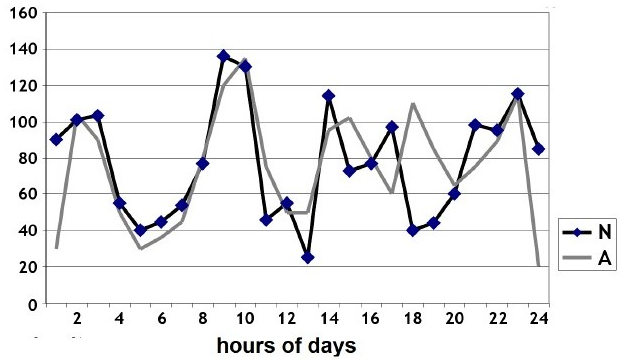
\includegraphics[width=70mm]{figs/ex-tsd.png}
% \end{center}
% 
% 
% \end{frame}



\begin{frame}[c]
 \frametitle{Contributions}
 
 \begin{tikzpicture}[auto]
 
 \draw[thick, ->] (-3.5,0)--node[near end,above,rotate=90] {\scriptsize Niveau d'abstraction des dynamiques}(-3.5,8);
 
 \node[debutfin,align=center] (niv1) at (-2,7) {\begin{tikzpicture}[auto,scale=0.5] 
                                                 \path[use as bounding box] (-0.7,-0.3) rectangle (2.5,2);

                                                              \node[qgre,scale=0.5] (a) at (0,2) {a};
                                                              \node[mod,scale=0.5] (i) at (1,1) {i};
                                                              \node[qgre,scale=0.5] (b) at (0,0) {b};
                                                              \node[qgre,scale=0.5] (c) at (2,1) {c};
                                                              \path
                                                                (a) edge[inh,scale=0.1] (i)
                                                                (b) edge[act,scale=0.1] (i)
                                                                (i) edge[st,scale=0.1]  (c);
                                                              
                                                 \end{tikzpicture}};
                                                 
 \node[debutfin,align=center] (niv2) at (-2,4) {\begin{tikzpicture}[auto,scale=0.5] 
                                                 \path[use as bounding box] (-0.7,-0.3) rectangle (2.5,2);

                                                              \node[qgre,scale=0.5] (a) at (0,2) {a};
                                                              \node[mod,scale=0.5] (i) at (1,1) {i};
                                                              \node[qgre,scale=0.5] (b) at (0,0) {b};
                                                              \node[qgre,scale=0.5] (c) at (2,1) {c};
                                                              \path
                                                                (a) edge[inh,scale=0.1] (i)
                                                                (b) edge[act,scale=0.1] (i)
                                                                (i) edge[st,scale=0.1]  (c);
                                                                
                                                  \node[grandplus] (plus) at (1.2,0.2) {$+$};
                                                  \node[grandplus] (plus) at (2,0) {$K$};
                                                              
                                                 \end{tikzpicture}};
                                                
 \node[debutfin,align=center] (niv3) at (-2,1) {\begin{tikzpicture}[auto,scale=0.5] 
                                                 \path[use as bounding box] (-0.7,-0.3) rectangle (2.5,2);

                                                              \node[qgre,scale=0.5] (a) at (0,2) {a};
                                                              \node[mod,scale=0.5] (i) at (1,1) {i};
                                                              \node[qgre,scale=0.5] (b) at (0,0) {b};
                                                              \node[qgre,scale=0.5] (c) at (2,1) {c};
                                                              \path
                                                                (a) edge[inh,scale=0.1] (i)
                                                                (b) edge[act,scale=0.1] (i)
                                                                (i) edge[st,scale=0.1]  (c);
                                                                
                                                  \node[grandplus] (plus) at (1,0) {$+$};
                                                  \node[grandplus] (plus) at (2,0.5) {$K$};
                                                  \node[scale=0.5] (clock) at (2,-0.25) {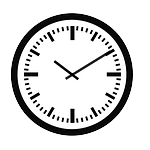
\includegraphics[scale=0.22]{figs/clock.png}};
                                                              
                                                 \end{tikzpicture}};
                                                 

 
 %\node[grandplus] (plus) at (2,0) {$+$};
 

 
 \draw[thick, ->] (7.8,8)--node[near end,below,rotate=90] {\scriptsize Précision des propriétés}(7.8,0); %ligne de la précision des propriétés 
 
 
 
 
 % liste des propriétés
 %general properties
 \node[instruct,align=center] (gp) at (5.8,7) {\begin{tabular}{c}
                                            {\scriptsize Propriétés générales: bornes} \\ 
                                            {\scriptsize sur le nbr d'attracteurs;}\\ {\scriptsize fonctionnalités,...}
                                           \end{tabular}};
 
 %fixed points
 \node[instruct,align=center] (fp) at (6.7,5.6) {\begin{tabular}{c}
                                                 {\scriptsize \'Etats stables}
                                                 \end{tabular}};
                                           
 %reachabilities
 \node[instruct,align=center] (reach) at (6.7,4) {\begin{tabular}{c} {\scriptsize Bifurcations} \\ {\scriptsize Accessibilité} \\ {\scriptsize (CTL)} \end{tabular}};
 \node[instruct,align=center] (qreach) at (6.7,1) {\begin{tabular}{c} {\scriptsize Accessibilité} \\ {\scriptsize quantitative} \\{\scriptsize (CCSL)} \end{tabular}};
 
 
 %process hitting
 

 
 
 
 \uncover<1->{
 
% \begin{pgfonlayer}{background}
 \draw[->,color=gray!10,bend right,line width=4pt,round] (niv3)--node[near center,below] {\scriptsize }(qreach);
 
 \draw[->,color=gray!10,bend right,line width=0.5pt] (niv1)-- (gp);
 
  \draw[->,color=gray!10,bend right,line width=0.6pt,round] (niv2)--node[near center,below] {\scriptsize }(fp);
 
 \draw[->,color=gray!10,bend right,line width=2pt,round] (niv2)--node[near center,below] {\scriptsize }(reach);
% \end{pgfonlayer}
 
   
 %ajout de la notion de chronométrie
 \draw[gray!80,loosely dashed] (-4,2.5) -- node[very near start,below] {\scriptsize Chronométrie}node[very near start,above] {\scriptsize Chronologie}(8,2.5);

 
 }
 
 \uncover<1->{
 \node[es,align=center] (ph) at (2,4.5) {\begin{tabular}{c}
                                           {\scriptsize \textbf{Réseaux} }\\ 
                                           {\scriptsize \textbf{d'automates}}
                                           \end{tabular}};
 \node[instruct,align=center] (pint) at (2,3) {\scriptsize PINT};
 \draw[->,dashed] (ph)--(pint);
 }
 
 
 %les relations
 \uncover<1->{
 \draw[suite,color=gray] (niv1)--(ph);
 \draw[suite,color=gray] (niv2)--(ph);
  \draw[suite,line width=0.5pt,color=gray] (ph)--node[near center,above,rotate=18] {\scriptsize Analyse statique}(fp);
 \draw[suite,color=darkblue] (niv3)--node[near center,above,bend right,rotate=45] {\scriptsize Modélisation}node[inner,below]{1.A}(ph);
 \draw[suite,blue!60,round]     (pint) --node[near center,above,bend right,rotate=90] {\scriptsize Simulation}node[inner,right]{1.B}(2,1.5)-- node[near center,above,bend right] {\scriptsize Analyse} (niv3);
 \draw[suite,color=blue!60] (ph)--node[near center,above,rotate=-35] {\scriptsize Analyse statique}node[inner,below]{2}(qreach);
  \draw[suite,blue!60] (ph)--node[near center,above,blue!60,rotate=-5] {\scriptsize Analyse statique}node[inner,below]{3}(reach);
 }
 
  \uncover<2->{
  \draw[suite,color=darkblue,line width=2pt] (niv3)--node[near center,above,bend right,rotate=45] {\scriptsize Modélisation}node[inner,below]{1.A}(ph);
 }
 
  
 \end{tikzpicture}

 
\end{frame}

% %mettre la transition
\section{Raffinement de la dynamique par intégration des séries temporelles}
 
\begin{frame}[c]
 \frametitle{Modélisation hybride}
 %\framesubtitle{Concept}
  %\pause
 %figure illustrative
 \begin{tikzpicture}[auto]
  
\path[use as bounding box] (-0.7,-2) rectangle (3,3);

%le noeud pour les connaissances de la littérature, générales
\node[align=center] (gk) at (2,3) {\begin{tabular}{|c|} 
\hline
 Connaissances générales  \\
 \hline
 Littérature  \\
  \hline
 Hypothèses   \\
  \hline
\end{tabular}};

%\pause

%les noeud pour le réseau biologique
\node[qgre] (a) at (1,1.5) {a};
\node[mod] (i) at (2,1) {i};
\node[qgre] (b) at (1,0.5) {b};
\node[qgre] (c) at (2.5,1) {c};


\path
 (a) edge[act] (i)
 (b) edge[inh] (i)
 (i) edge[st]  (c);
 
 %\pause

\node (deco) at (2,-0.1) {Données de séries temporelles};
\node[align=center] (tsd) at (2,-1) {\begin{tabular}{|c|c|c|c|} 
\hline
 Genes  & 1h & ... & 24h  \\
 \hline
 Gene $1$  &   & ...  &    \\
  \hline
  Gene $2$  &   & ...  &    \\
  \hline
\end{tabular}};


\onslide<2->{

\node (d1) at (5,1) {};
\node (d2) at (7.5,1) {};

\node (d3) at (4.5,-1.5) {};
\node (d4) at (4.5,3.5) {};


\draw[->,line width=6pt, color=lightgray] (d1) -- (d2) node[above=10pt,midway]{\textcolor{black}{\textbf{Modélisation algébrique}}};
}



%\draw[decoration={brace,amplitude=12pt}, 
%decorate,line width=2pt,gray] (d3) -- (d4) node[above=10pt,midway]{\textcolor{black}{\textbf{}}};


\onslide<2->{
%le modèle en process hitting
\node[scale=0.4] (phmodel) at (10,1) {\begin{tikzpicture} \exphHM 
                           \end{tikzpicture}};
}

\end{tikzpicture}

\onslide<2->{
 \begin{block}
  
  \begin{itemize}
   \item Caractérisation formelle de la topologie et de la dynamique des RRB.
   \item Intégration des données de séries temporelles.
   \item Raffinement qualitatif et quantitatif de la dynamique.
   \item Simulation stochastique et analyse statistique des traces.
  \end{itemize}

 \end{block}
}

\end{frame}

 
%\usepackage{tikz}


\begin{frame}[c]
%\frametitle{Approche}
\begin{tikzpicture}[grn]

 % placement des noeuds
 
  \node[es,align=center] (rstc) at (-2,5) {\begin{tabular}{c}
                                            \textbf{Réseaux biologiques} \\ \hline
                                            Réseaux  RSTC
                                           \end{tabular}};
  
  \node[es] (data) at (4,5) {\begin{tabular}{c}
                                            \textbf{Données expérimentales} \\ \hline
                                            Séries temporelles (TSD)
                                           \end{tabular}};
  
 \node[instruct,align=center] (phmodel) at (-2,2.5) {\begin{tabular}{c}
                                            \textbf{Modèles hybrides} \\ \hline
                                            Modèles AN
                                           \end{tabular}};
                                           
  \node[instruct] (estimation) at (2.5,2.5) {\begin{tabular}{c}
                                            \textbf{Estimation des paramètres}\\ \hline
                                            $r$ et $sa$ 
                                           \end{tabular}};
                                           
   
  \node[instruct] (discretization) at (6.5,2.5) {\begin{tabular}{c}
                                            \textbf{Discrétisation} \\ \hline
                                            TSD
                                           \end{tabular}};
                                           
  \node[instruct] (simulation) at (-2,0) {\begin{tabular}{c}
                                           \textbf{Simulation}\\ 
                                           PINT
                                          \end{tabular}};
    
  
  \node[test] (test) at (3,0) {Validation du modèle};
  
 %placement des arrêtes
  \draw[suite] (rstc) -- (phmodel);
  \draw[suite] (phmodel) -- (simulation);
  \draw[suite] (simulation) -- (test.west);
  
  \draw[suite] (data) -- (estimation);
  \draw[suite] (estimation) -- (phmodel);
  \draw[suite] (data) -- (discretization);
  \draw[suite] (discretization) -- (test.east);
\end{tikzpicture}

\end{frame}

 \subsection{Les données}
 \begin{frame}[c]
 \frametitle{Réseau type RSTC}
 \framesubtitle{multi-layer Receptor-Signaling-Transcription-Cell state\\
 {\tiny \color{darkgreen} [\citecaritofebs]}

 }

\begin{center}
  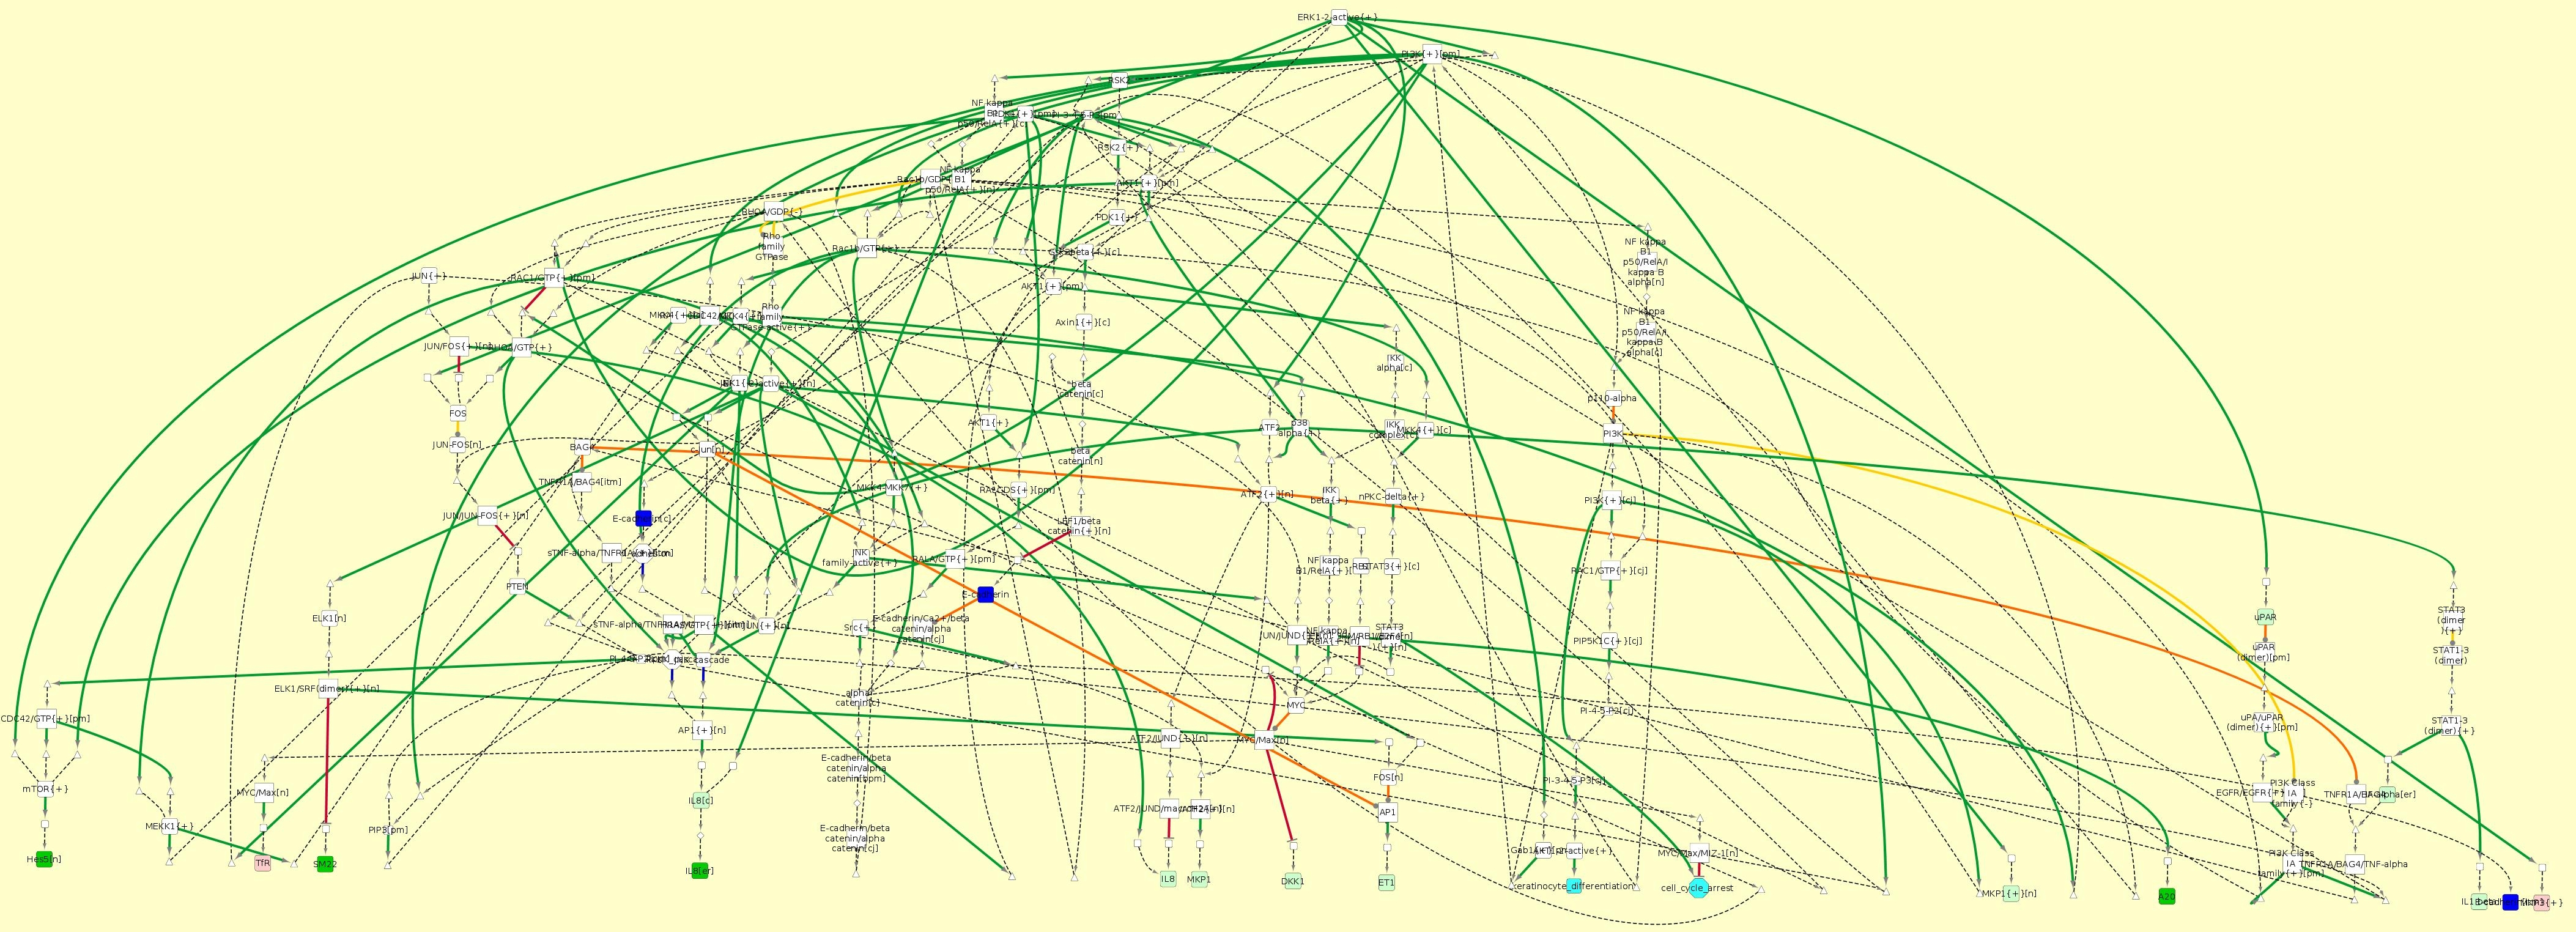
\includegraphics[scale=0.07]{figs/net.jpg}
\end{center}
 

\begin{itemize}
 \item Cas d'étude \tval{Ecad} extrait de Pathway Interaction Database (PID).
 \item \tval{$293$  n{\oe}uds}: protéines de signalisation, facteurs de transcription, gènes,...
 \item \tval{$375$  interactions}: activations, inhibitions, dissociation des  complexes,...
\end{itemize}

 
\end{frame}

\begin{comment}
\begin{frame}[c]
 \frametitle{Réseaux RSTC}
 \framesubtitle{multi-layer receptor-signaling-transcription-cell state}

%%%image zoomée
\begin{tikzpicture}[node distance = 1em,dashed,red,thick]
	\zoomZero{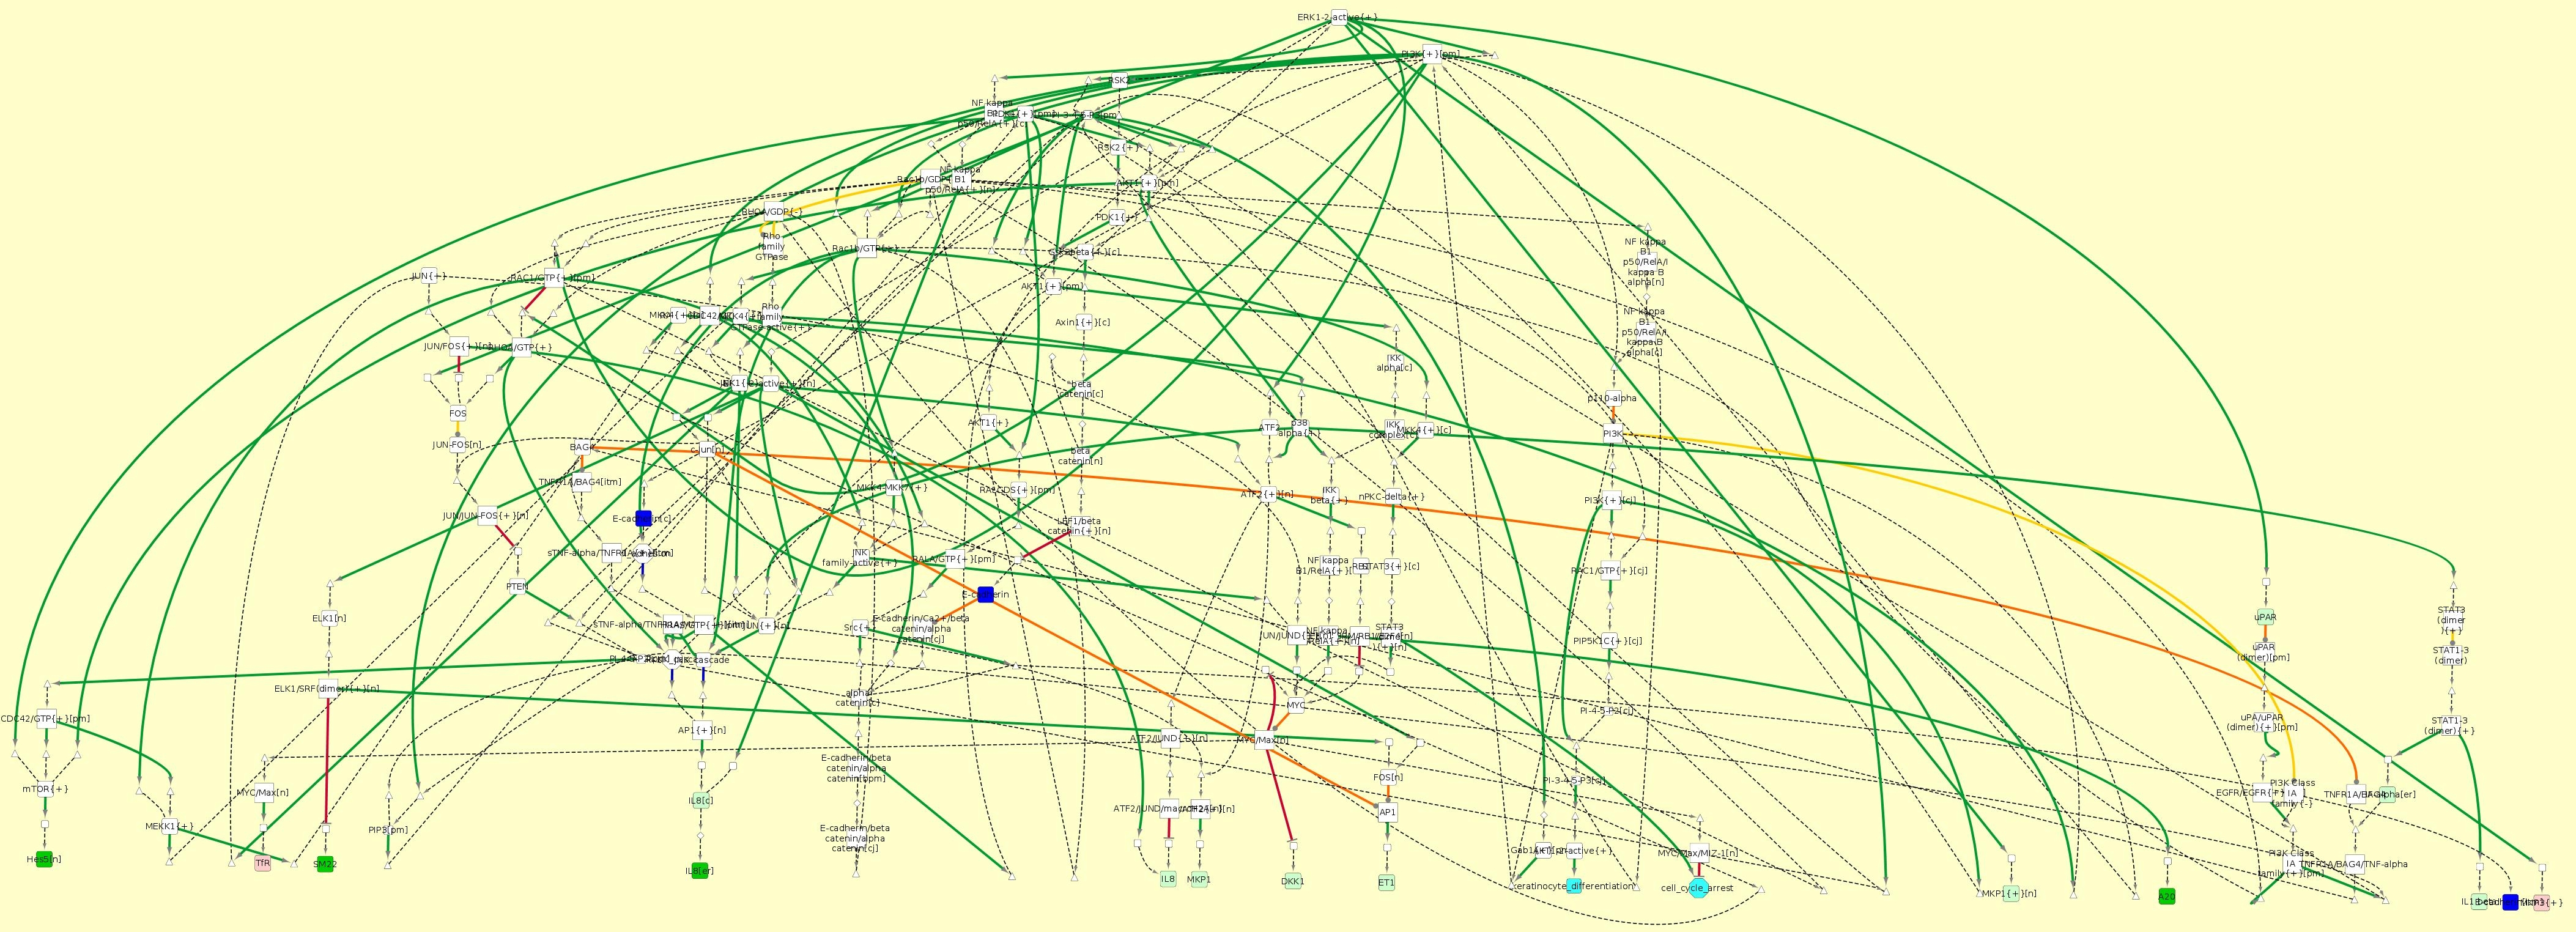
\includegraphics[width=0.35\textwidth]{figs/net.jpg}}
	\zoomIn[right]{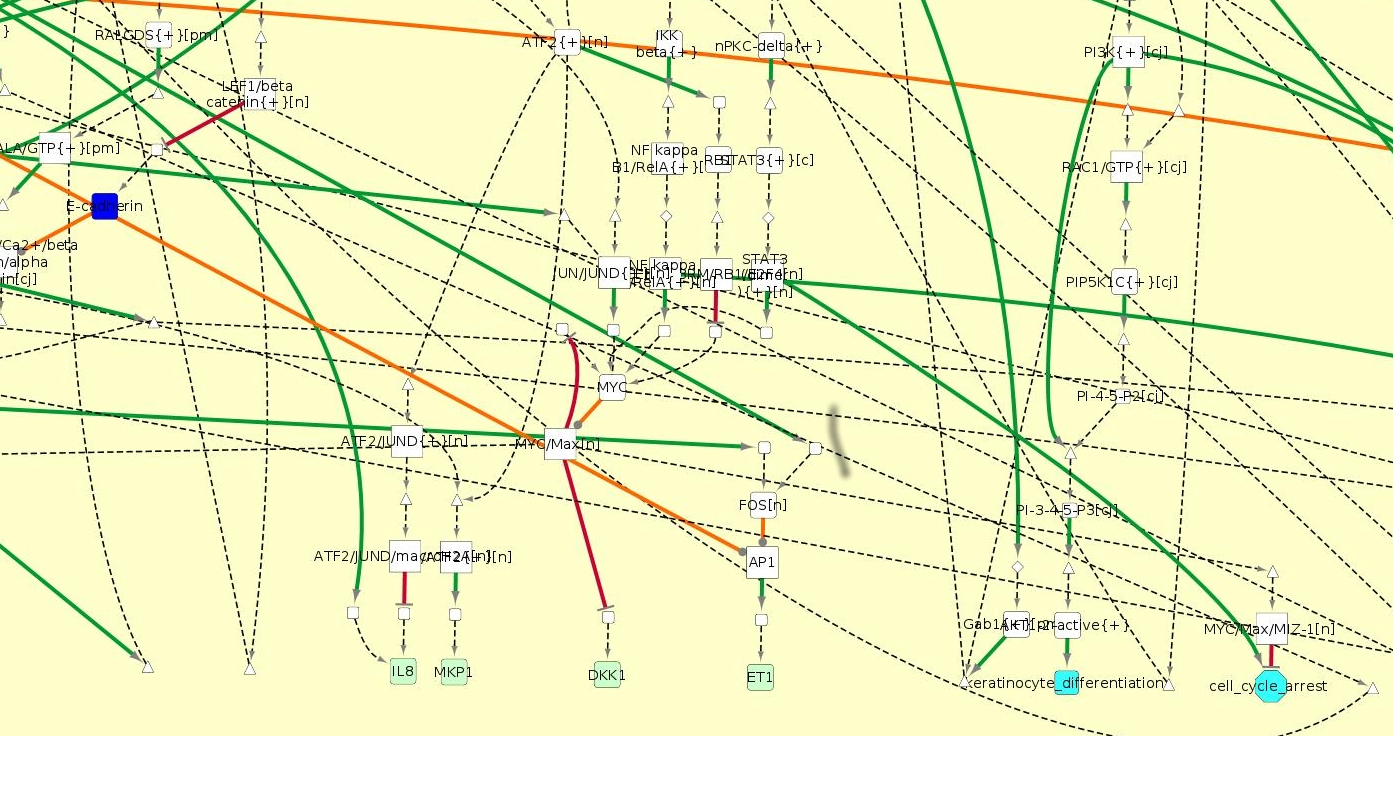
\includegraphics[scale=0.15]{figs/netzoom.png}}{0.35,0.005}{0.320,0.420}
	%\zoomIn{\includegraphics[width=0.45\textwidth]{Geant3}}{0.45,0.475}{0.120,0.120}
	%\zoomIn[left]{\includegraphics[width=0.45\textwidth]{Geant2}}{0.45,0.475}{0.120,0.120}
	%\zoomIn{\includegraphics[width=0.45\textwidth]{Geant1}}{0.45,0.475}{0.120,0.120}
	%\zoomIn[right]{\includegraphics[width=0.45\textwidth]{Geant0}}{0.45,0.475}{0.120,0.120}
\end{tikzpicture}


\end{frame}

\begin{frame}[c]
 \frametitle{RSTC Network}
 \framesubtitle{multi-layer receptor-signaling-transcription-cell state}

%%%image zoomée
\begin{tikzpicture}[node distance = 1em,dashed,red,thick]
	\zoomZero{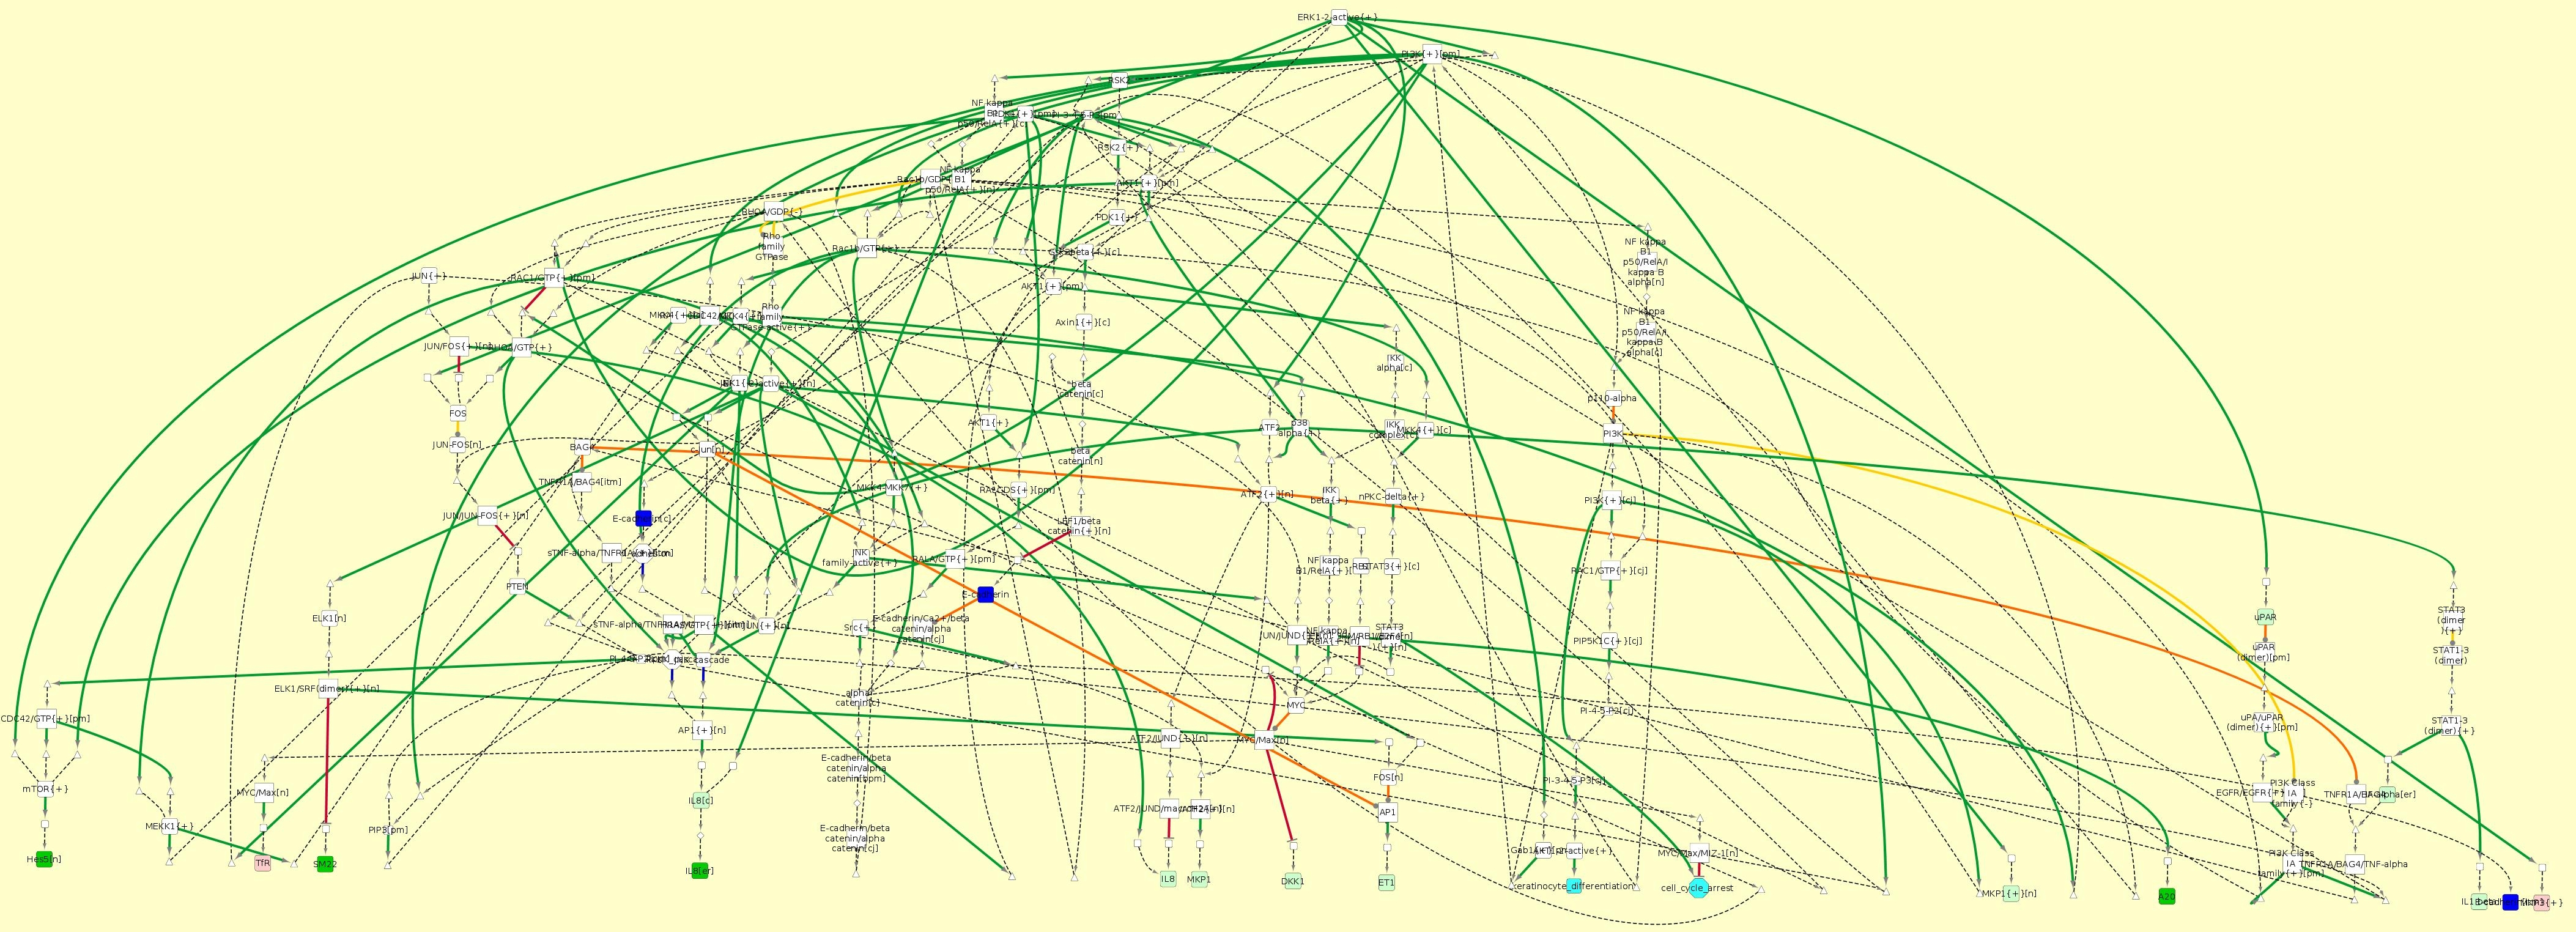
\includegraphics[width=0.45\textwidth]{figs/net.jpg}}
	\zoomIn[left]{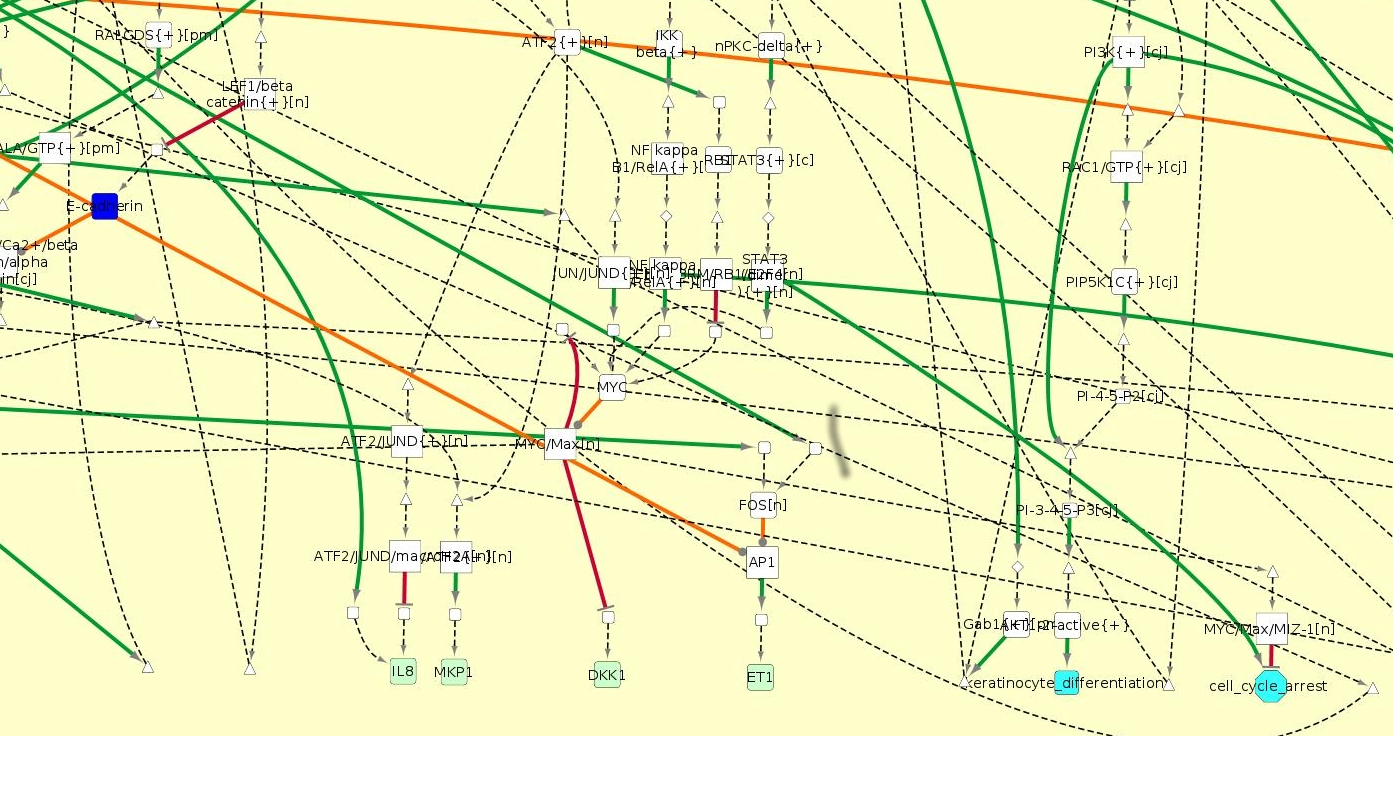
\includegraphics[scale=0.25]{figs/netzoom.png}}{0.35,0.005}{0.320,0.420}
	%\zoomIn{\includegraphics[width=0.45\textwidth]{Geant3}}{0.45,0.475}{0.120,0.120}
	%\zoomIn[left]{\includegraphics[width=0.45\textwidth]{Geant2}}{0.45,0.475}{0.120,0.120}
	%\zoomIn{\includegraphics[width=0.45\textwidth]{Geant1}}{0.45,0.475}{0.120,0.120}
	%\zoomIn[right]{\includegraphics[width=0.45\textwidth]{Geant0}}{0.45,0.475}{0.120,0.120}
\end{tikzpicture}


\end{frame}
\end{comment}

 \begin{frame}[c]
  \frametitle{Données de séries temporelles (TSD)}
  \framesubtitle{{\small \color{darkgreen} [\citedata]}}
  
\begin{center}
  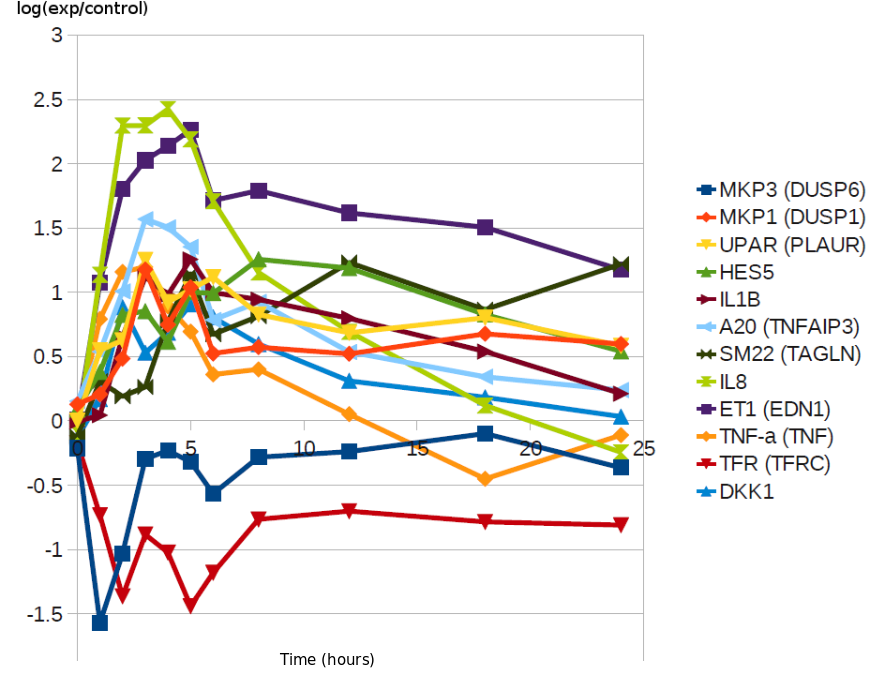
\includegraphics[width=70mm]{figs/12genes.png}
\end{center}

%\pause

\begin{columns}
\begin{column}{0.7\textwidth}
\begin{itemize}
  \item Expérience: \tval{stimulation au calcium} d'Ecad.
  \item Mesurer à  $10$ intervalles de temps (0-24hrs).
  \item Sélection de \tval{$200$ transcripts}  (\tval{dynamique}). %their fold expression with respect to the non-stimulated cell was significant in at least one time point
  %\item Nous avons inclu $12$ mRNA dans notre modèle.
\end{itemize}
\end{column}

\begin{column}{0.3\textwidth}
% \textbf{ \small Prof. Dr. Peter Angel
%Signal Transduction and Growth Control (A100)
%German Cancer research center
%Heidelberg, Germany}

\end{column}
\end{columns}
%\textcolor{couleurtheme}{$\Rightarrow$} \fbox{\tval{\large Allow efficient translation from Process Hitting to BRN}} \textcolor{couleurtheme}{$\Leftarrow$}

\end{frame}



 \subsection{Formalisation des RSTC comme des réseaux d'automates}
 %%explain the automatic model construction

%mettre un RRB ----> en AAN  ----> STate graph 
%rajouter une slide
\begin{frame}
\frametitle{Modélisation des RSTC par les réseaux d'automates (AN)}
\begin{tikzpicture}
 \node[scale=1] (brn) at (0,5) {\begin{tikzpicture}[auto,scale=0.9] 
                                                  \path[use as bounding box] (-0.7,-0.3) rectangle (2.5,2);
 
                                                               \node[qgre,scale=0.8] (a) at (0,2) {a};
                                                                \node[mod,scale=0.8] (i) at (1,1) {i};
                                                                \node[qgre,scale=0.8] (b) at (0,0) {b};
                                                                \node[qgre,scale=0.8] (c) at (2,1) {c};
                                                                \path
                                                                  (a) edge[act,scale=0.1] (i)
                                                                  (b) edge[inh,scale=0.1] (i)
                                                                  (i) edge[st,scale=0.1]  (c)
                                                                  ;
                                                               
                                                  \end{tikzpicture}};
%\node (brn) at (0,5) {};
\node[scale=0.6] (an) at (7,5) {\begin{tikzpicture}
\exandef
\end{tikzpicture}};
\node[scale=0.4] (sg) at (2,1) {
\begin{tikzpicture}[line join=bevel,font=\LARGE]
%%
  \node (6) at (405.0bp,18.0bp) [reach,nd4] {$\langle a_2,b_1,c_0\rangle$};
  \node (2) at (405.0bp,90.0bp) [reach,nd3] {$\langle a_2,b_0,c_0\rangle$};
  \node (1) at (570.0bp,90.0bp) [reach,nd1] {$\langle a_1,b_0,c_0\rangle$};
  \node (0) at (469.0bp,162.0bp) [reach,nd0] {$s_0 = \langle a_0,b_0,c_0\rangle$};
  \node (4) at (469.0bp,234.0bp) [reach,nd5] {$\langle a_0,b_1,c_0\rangle$};
 
 
  \draw [->,arc3] (0) ..controls (445.65bp,135.46bp) and (435.95bp,124.86bp)  .. (2);
  \draw [->,arc5] (0) ..controls (475.71bp,188.03bp) and (475.94bp,197.36bp)  .. (4);
  \draw [->,arc4] (2) ..controls (405.0bp,63.983bp) and (405.0bp,54.712bp)  .. (6);
  \draw [->,arc1] (0) ..controls (499.93bp,134.79bp) and (517.41bp,122.58bp)  .. (1);
  \draw [->,arc2] (1) ..controls (539.0bp,117.26bp) and (521.52bp,129.47bp)  .. (0);
  \draw [->,arc5] (4) ..controls (462.3bp,208.35bp) and (462.06bp,199.03bp)  .. (0);
 
%
\end{tikzpicture}

};
\path 
(brn) edge[->,line width=8pt, color=lightgray] (an)
(an) edge[->,line width=8pt, color=lightgray,bend left] (sg)
;
\end{tikzpicture}
\end{frame}




\begin{frame}[c]
\frametitle{Formalisation des réseaux RSTC}
\framesubtitle{Détection et transformation automatique des motifs minimaux}

%We have two procedures that allow us to detect and translate RSTC network to the Process Hitting model.

\begin{tikzpicture}[auto]
 
 % placement des noeuds
 
 %\node[cloud, cloud puffs = 10, draw, minimum width = 0.1cm, minimum height = 0.1cm, fill = gray!10, scale=0.3] (rstcbis) at (-2,13){
 %  \begin{tabular}{c}
 %  \textbf{Biological network} \\ \hline
 %  RSTC network
 % \end{tabular}};
 \node (rep2) at (0,12) {};
 \node (rep) at (0,-5) {};
  
  \node[es,align=center,scale=0.5] (rstcbis) at (-2,11.5) {\begin{tabular}{c}
                                            \textbf{Réseau biologique} \\ \hline
                                            réseau  RSTC 
                                           \end{tabular}};

 
\onslide<2->{
%\draw[-open triangle 90] (0,12.5) -- (0.2,12.5);
 \node[instruct,align=center, scale=0.7] (pro1) at (0.5,11.5) {\begin{tabular}{c}
                                            \textbf{Détection des motifs} \\ \hline
                                            dans les  RSTC network
                                          \end{tabular}};
      
 \path
  (rstcbis) edge[st] (pro1);
}
                                          
 \onslide<3->{
 %\draw[-open triangle 90] (2,12.5) -- (2.5,12.5);
 \node[es, scale=0.5] (sop) at (3,11.5) {\begin{tabular}{c}
                                            \textbf{Ensemble de motifs} \\ \hline
                                            du réseau RSTC
                                           \end{tabular}};

\path
   (pro1) edge[st] (sop);
                                           
\node[scale=0.8] (bpat) at (-1,8) {\begin{tabular}{|c|}
\hline
\textbf{Motifs biologiques}

\\ \hline
\begin{tikzpicture}
\node[scale=0.7] (sa1) at (0,0){\begin{tikzpicture}[auto]
\path[use as bounding box] (-0.7,-0.3) rectangle (2.5,2);

\node[qgre] (a) at (0,0.5) {a};
\node[mod] (i) at (1,0.5) {i};
\node[qgre] (b) at (2,0.5) {b};
\node[es] (d) at (1,1.5) {Simple activation};

% a restorer
\path
 (a) edge[act] (i)
 (i) edge[st]  (b);
\end{tikzpicture}};
\end{tikzpicture}

\\ \hline

\begin{tikzpicture}
\node[scale=0.7] (si1) at (0,0){\begin{tikzpicture}[auto]
\path[use as bounding box] (-0.7,-0.3) rectangle (2.5,2);

\node[qgre] (a) at (0,0.5) {a};
\node[mod] (i) at (1,0.5) {i};
\node[qgre] (b) at (2,0.5) {b};
\node[es] (d) at (1,1.5) {Simple inhibition};

%a restorer 
\path
 (a) edge[inh] (i)
 (i) edge[st]  (b);
 \end{tikzpicture}};
\end{tikzpicture}


\\ \hline

\begin{tikzpicture}
\node[scale=0.7] (sai1) at (0,0){\begin{tikzpicture}[auto]
\path[use as bounding box] (-0.7,-0.3) rectangle (2.5,3);
\node[qgre] (a) at (0,2) {a};
\node[mod] (i) at (1,1) {i};
\node[qgre] (b) at (0,0) {b};
\node[qgre] (c) at (2,1) {c};
\node[es] (d) at (1,2.5) {activation ou inhibition};

% arestorer
\path
 (a) edge[act] (i)
 (b) edge[inh] (i)
 (i) edge[st]  (c);
\end{tikzpicture}};
\end{tikzpicture}

\\ \hline

\end{tabular}
};

}


\onslide<4->{

\node[es,scale=0.5] (timed) at (3,10.5) {\begin{tabular}{c}
                                            \textbf{Délai} \\ \hline
                                            Estimation des TSD
                                           \end{tabular}};


 \node[instruct,align=center, scale=0.7] (pro2) at (6,11.5) {\begin{tabular}{c}
                                            \textbf{Transformation des motifs} \\ \hline
                                            en  AN modèle
                                           \end{tabular}};
 \path
    (sop) edge[st] (pro2)
    (timed) edge[st] (pro2);
 }
 
 \onslide<5->{
   
   \node[es,scale=0.5] (php) at (8.7,11.5) {\begin{tabular}{c}
                                            \textbf{AN motifs} \\
                                           \end{tabular}};
\path
   (pro2) edge[st] (php);

\node[scale=0.8] (phpat) at (6.8,8) {\begin{tabular}{|c|c|}
\hline

\textbf{AN Transformations}

 \\ \hline

\begin{tikzpicture}
%\exphpatact
\node[scale=0.5] (sa) at (0,0) {\begin{tikzpicture}
\exphpatact
\end{tikzpicture}};
\end{tikzpicture}


\\ \hline


\begin{tikzpicture}
%\exphpatact
\node[scale=0.5] (sa) at (0,0) {\begin{tikzpicture}
\exphpatini
\end{tikzpicture}};
\end{tikzpicture}

 \\ \hline


\begin{tikzpicture}
%\exphpatact
\node[scale=0.5] (sai) at (0,0) {\begin{tikzpicture}
\exphpatai
\end{tikzpicture}};
\end{tikzpicture}
\\ \hline

\end{tabular}
};
}
\end{tikzpicture}

%exemple of patterns 


\end{frame}


\begin{frame}[t]
 \frametitle{Formalisation des réseaux RSTC}
 \framesubtitle{Détection automatique des motifs minimaux} 

\begin{columns}
\begin{column}{0.6\textwidth}

\begin{tikzpicture}[auto]

\node[qgre] (a1) at (-3,-3) {a};
\node[qgre] (a2) at (-1,-3) {b};
\node[qgre] (a3) at (1,-3) {c};
\node[qgre] (a4) at (3,-3) {d};
%\node[qgre] (a5) at (5,-3) {e};

\node[mod] (i1) at (-3,-2) {};
\node[mod] (i2) at (-1,-2) {};
\node[mod] (i3) at (1,-2) {};
\node[mod] (i4) at (3,-2) {};
%\node[mod] (i5) at (5,-2) {};

\node[ps] (ps1) at (-3,-1) {PS1};
\node[ps] (ps2) at (-1,-1) {PS2};
\node[ps] (ps3) at (1,-1) {PS3};
\node[ps] (ps4) at (3,-1) {PS4};
%\node[ps] (ps5) at (5,-1) {PS5};

\node[mod] (i6) at (-3,0) {};
%\node[mod] (i7) at (-1,0) {};
\node[mod] (i8) at (1,0) {};
\node[mod] (i9) at (3,0) {};
%\node[mod] (i10) at (5,0) {};

\node[ps] (ps6) at (-3,1) {PS6};
%\node[ps] (ps7) at (-1,1) {PS7};
\node[ps] (ps8) at (1,1) {PS8};
\node[ps] (ps9) at (3,1) {PS9};
%\node[ps] (ps10) at (5,1) {PS10};

%les complex
\node[ecad] (d) at (0,3) {Input};
\node[cplx] (c1) at (2,-1) {cplx1};
\node[cplx] (c2) at (0,1) {cplx2};
\node[cplx] (c3) at (-2,-1) {cplx3};
\node[cplx] (c4) at (-2,1) {cplx4};
\node[cplx] (c5) at (0,0) {cplx5};
\node[cplx] (c6) at (2,1) {cplx6};

%les seed node
\node[sn] (sn1) at (-2,-3) {SN1};
\node[sn] (sn2) at (2,-3) {SN2};


%les edges 

\path
 (i1) edge[st] (a1)
 (i2) edge[st] (a2)
 (i3) edge[st]  (a3)
 (i4) edge[st]  (a4)
 %(i5) edge[st]  (a5)
 
 (ps1) edge[act] (i1)
 (ps2) edge[act] (i2)
 (ps3) edge[act] (i2)
 (ps3) edge[act] (i3)
 (ps4) edge[act] (i4)
 %(ps5) edge[act] (i5)
 
 (i6) edge[st] (ps1)
 (i6) edge[st] (ps2)
 (i8) edge[st] (ps3)
 (i9) edge[st] (ps4)
 (i9) edge[st] (ps4)
 %(i9) edge[st] (ps5)
 %(i10) edge[st] (ps5)
 
 (ps6) edge[act] (i6)
 (ps8) edge[act] (i8)
 (ps9) edge[act] (i9)
 %(ps10) edge[act] (i10)
 
 (d) edge[act] (ps6)
 (d) edge[act] (ps8)
 (d) edge[act] (ps9)
 %(d) edge[act] (ps10)
 
 (c4) edge[act] (c5)
 (c2) edge[act] (c5)
 (d) edge[act] (c2)
 (c5) edge[inh] (ps2)
 (c6) edge[act] (i8)
 (c6) edge[act] (i9)
 (i8) edge[st] (c1)
 (i9) edge[st] (c1)
 (c1) edge[act] (i4)
 
 (ps3) edge[inh] (sn2)
 (i4) edge[st] (sn2)
 
 (ps1) edge[inh] (sn1)
 (c3) edge[act] (sn1)
 (c4) edge[act] (c3)
 
 (a1) edge[inh, bend left] (ps6);
 

 %pattern 1
\only<2->{
\node[snpat] (snpat1) at (1,-3) {};
}
\only<3->{
\path
 (a3) edge[stv] (i3);
 }
 \only<4->{
\path
 (i3) edge[stv] (ps3);
 }
  \only<5->{
\node[snpat] (snpat2) at (1,-1) {};
}

  %le pattern rajouté
% \only<5-9>{
% \node[scale=0.9] (patraj1) at (5,-2){\begin{tikzpicture}[auto]
% \path[use as bounding box] (-0.7,-0.3) rectangle (2.5,2);
% 
% \node[ps] (aps3) at (0,0.5) {PS3};
% \node[mod] (ips3) at (1,0.5) {i};
% \node[qgre] (cps3) at (2,0.5) {c};
% 
% % a restorer
% \path
%  (aps3) edge[act] (ips3)
%  (ips3) edge[st]  (cps3);
% \end{tikzpicture}};
% 
% }

%pattern 2

%le pattern rajouté
% \only<9>{
% \node[scale=0.9] (sai1) at (5,-3.5){\begin{tikzpicture}[auto]
% \path[use as bounding box] (-0.7,-0.3) rectangle (2.5,3);
% \node[ps] (aps2) at (0,2) {PS2};
% \node[mod] (ips2) at (1,1) {i};
% \node[ps] (bps3) at (0,0) {PS3};
% \node[qgre] (cb) at (2,1) {b};
% 
% % arestorer
% \path
%  (aps2) edge[act] (ips2)
%  (bps3) edge[act] (ips2)
%  (ips2) edge[st]  (cb);
% \end{tikzpicture}};
% 
% 
% }

 \only<6->{
\node[snpat] (snpat3) at (-1,-3) {};
}


 \only<7->{
\path
 (a2) edge[stv] (i2);
 }
 \only<8->{
\path
 (i2) edge[stv] (ps2)
 (i2) edge[stv] (ps3);
 }
 
  \only<9->{
\node[snpat] (snpat4) at (-1,-1) {};
\node[snpat] (snpat5) at (1,-1) {};
}


%pattern 3 qui n'est pas un pattern

 
\end{tikzpicture}

\end{column}

\begin{column}{0.4\textwidth}

 \begin{liste}
  \item \tval{N{\oe}uds terminaux:} protéines, complexes, gènes, états cellulaires,...
  \item \tval{N{\oe}uds transitoires:} translocations, modifications, transcriptions,...
 \end{liste}
 
 \uncover<10->{
 \tval{Complexité}:
  \tval{$\mathcal{O}(|V|\log{}(h))$}. 
  avec 
  \begin{liste}
 % \item \tval{$|V|$} est l'ensemble des n{\oe}uds et \tval{$|E|$} est l'ensemble des arcs.
 % \item $h$ est la hauteur moyenne des motifs dans le réseau RSTC. Dans le pire des cas 
 \item
  $h$ = hauteur moyenne des motifs.
 \end{liste}
 }
 
 \begin{center}%
\vspace*{1cm}%
\uncover<1->{%
\scalebox{\scaleex}{%
\begin{tikzpicture}[aS]
  \path[use as bounding box] (.7,1) rectangle (5.8,2.5);

  \glclegend{$g$}{$c$}{$s$}
\end{tikzpicture}
}
}
\end{center}

 
\end{column}



\end{columns}

\end{frame}



 \subsection{Estimation et intégration des paramètres temporels et stochastiques}
 
\begin{frame}[c]
 \frametitle{Estimation du taux des séries temporelles}
 %\framesubtitle{Estimation des  paramètres temporels}
 
\begin{columns}

\begin{column}{0.7\textwidth}
\scalebox{0.9}{
\begin{tikzpicture}[scale = 0.8]
    % Tracé de la parabole
    %\draw[red, domain = -2.2:2.2, smooth] plot (\x, {(\x)^2});
    % Alternative par Gnuplot
    %\draw[red, domain = -2.2:2.2, smooth] plot function{x**2};
    % Lignes tiretées
      \draw[thick, ->] (-.2,0)--(11,0) node[below]{$t$};
     \foreach \t in {0,1,2,3,4,...,10}
      \draw[very thick] (\t,2pt)--(\t,-2pt);

     \draw[thick, ->] (0,-.2)--(0,4) node[left]{$b$};
     \foreach \y in {1,2,3}
      \draw[very thick] (2pt,\y)--(-2pt,\y) ;
      
    \draw[thick] plot[mark=ball,mark size=1pt] file {illustration.txt};
    
    \onslide<2->{
    \draw[thick,color=white] (2.8,3.5) -- (3.2,3.5) node[above,blue]{$Max$};
    \draw[thick,color=white] (2.8,-.2) -- (3.2,-.2) node[below,blue]{$Min$};
    }
    \onslide<3->{
    \draw[thick,|<->|] (3,0) -- (3,3.5);
    }
    \onslide<4->{
    \draw[thick,dotted,blue] (0,1.16) -- (10,1.16) node[right]{$s_1$}; 
    \draw[thick,dotted,blue] (0,2.33) -- (10,2.33) node[right]{$s_2$}; 
    }
    \onslide<5->{
    \draw[thick,dotted,purple] (0.7,1.16) -- (0.7,-.5) node[below]{$t_{1}$};
    }
    \onslide<6->{
    \draw[thick,dotted,purple] (1.5,2.33) -- (1.5,-.3) node[below]{$t_{2}$};
    }
    \onslide<7->{
    \draw[thick,dotted,purple] (4.2,2.33) -- (4.2,-.3) node[below]{$t_{3}$};
    }
    \onslide<8->{
    \draw[thick,dotted,purple] (9.4,1.16) -- (9.4,-.3) node[below]{$t_{4}$};
    }
\end{tikzpicture}
}
%If we assume that $t_{0}=0$,\\
\onslide<5->{$\PHfrappe{a_1}{b_0}{b_1}$ avec $r_{1}=\frac{1}{t_{1}-t_{0}}$\\}
\onslide<6->{$\PHfrappe{a_1}{b_1}{b_2}$ avec $r_{2}=\frac{1}{t_{2}-t_{1}}$\\}
\onslide<7->{$\PHfrappe{a_0}{b_2}{b_1}$ avec $r_{3}=\frac{1}{t_{3}-t_{2}}$\\}
\onslide<8->{$\PHfrappe{a_0}{b_1}{b_0}$ avec $r_{4}=\frac{1}{t_{4}-t_{3}}$\\}
\onslide<8->{Généralisation:  
\tval{ \Large {$r_{i}=\frac{1}{t_{i}-t_{i-1}}$}}}
\end{column}

\begin{column}{0.3\textwidth}
\scalebox{0.9}{
 \begin{tikzpicture}[scale=0.8]
\path[use as bounding box] (-1,-1) rectangle (2,2);


\TSort{(0,1)}{b}{3}{r}


\only<5->{\TSort{(2,1)}{a}{2}{l}}
\only<5>{
\THit{a_1}{}{b_0}{.east}{b_1}
%\THit{a_0}{out=-120,in=180,selfhit}{a_0}{.west}{a_1}
\path[bounce]
%\TBounce{a_0}{bend left}{a_1}{.south}
\TBounce{b_0}{bend right}{b_1}{.south}
;
\TState{5}{a_1,b_0}
\TState{5}{a_1,b_1}
}

%deuxième estimation
\only<6>{
\THit{a_1}{}{b_1}{.east}{b_2}
%\THit{a_0}{out=-120,in=180,selfhit}{a_0}{.west}{a_1}
\path[bounce]
%\TBounce{a_0}{bend left}{a_1}{.south}
\TBounce{b_1}{bend right}{b_2}{.south}
;
\TState{6}{a_1,b_1}
\TState{6}{a_1,b_2}
}

%troisième  estimation
\only<7>{
\THit{a_0}{}{b_2}{.east}{b_1}
%\THit{a_0}{out=-120,in=180,selfhit}{a_0}{.west}{a_1}
\path[bounce]
%\TBounce{a_0}{bend left}{a_1}{.south}
\TBounce{b_2}{bend right}{b_1}{.north}
;
\TState{7}{a_0,b_2}
\TState{7}{a_0,b_1}
}

%troisième  estimation
\only<8>{
\THit{a_0}{}{b_1}{.east}{b_0}
%\THit{a_0}{out=-120,in=180,selfhit}{a_0}{.west}{a_1}
\path[bounce]
%\TBounce{a_0}{bend left}{a_1}{.south}
\TBounce{b_1}{bend right}{b_0}{.north}
;
\TState{8}{a_0,b_1}
\TState{8}{a_0,b_0}
}

\end{tikzpicture}
}

\end{column}
\end{columns}
\end{frame}

 
 
 \subsection{Simulations \& Validation}
 \begin{frame}[c]
 \frametitle{Contributions}
 
 \begin{tikzpicture}[auto]
 
 \draw[thick, ->] (-3.5,0)--node[near end,above,rotate=90] {\scriptsize Niveau d'abstraction des dynamiques}(-3.5,8);
 
 \node[debutfin,align=center] (niv1) at (-2,7) {\begin{tikzpicture}[auto,scale=0.5] 
                                                 \path[use as bounding box] (-0.7,-0.3) rectangle (2.5,2);

                                                              \node[qgre,scale=0.5] (a) at (0,2) {a};
                                                              \node[mod,scale=0.5] (i) at (1,1) {i};
                                                              \node[qgre,scale=0.5] (b) at (0,0) {b};
                                                              \node[qgre,scale=0.5] (c) at (2,1) {c};
                                                              \path
                                                                (a) edge[inh,scale=0.1] (i)
                                                                (b) edge[act,scale=0.1] (i)
                                                                (i) edge[st,scale=0.1]  (c);
                                                              
                                                 \end{tikzpicture}};
                                                 
 \node[debutfin,align=center] (niv2) at (-2,4) {\begin{tikzpicture}[auto,scale=0.5] 
                                                 \path[use as bounding box] (-0.7,-0.3) rectangle (2.5,2);

                                                              \node[qgre,scale=0.5] (a) at (0,2) {a};
                                                              \node[mod,scale=0.5] (i) at (1,1) {i};
                                                              \node[qgre,scale=0.5] (b) at (0,0) {b};
                                                              \node[qgre,scale=0.5] (c) at (2,1) {c};
                                                              \path
                                                                (a) edge[inh,scale=0.1] (i)
                                                                (b) edge[act,scale=0.1] (i)
                                                                (i) edge[st,scale=0.1]  (c);
                                                                
                                                  \node[grandplus] (plus) at (1.2,0.2) {$+$};
                                                  \node[grandplus] (plus) at (2,0) {$K$};
                                                              
                                                 \end{tikzpicture}};
                                                
 \node[debutfin,align=center] (niv3) at (-2,1) {\begin{tikzpicture}[auto,scale=0.5] 
                                                 \path[use as bounding box] (-0.7,-0.3) rectangle (2.5,2);

                                                              \node[qgre,scale=0.5] (a) at (0,2) {a};
                                                              \node[mod,scale=0.5] (i) at (1,1) {i};
                                                              \node[qgre,scale=0.5] (b) at (0,0) {b};
                                                              \node[qgre,scale=0.5] (c) at (2,1) {c};
                                                              \path
                                                                (a) edge[inh,scale=0.1] (i)
                                                                (b) edge[act,scale=0.1] (i)
                                                                (i) edge[st,scale=0.1]  (c);
                                                                
                                                  \node[grandplus] (plus) at (1,0) {$+$};
                                                  \node[grandplus] (plus) at (2,0.5) {$K$};
                                                  \node[scale=0.5] (clock) at (2,-0.25) {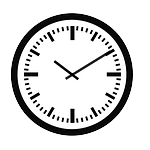
\includegraphics[scale=0.22]{figs/clock.png}};
                                                              
                                                 \end{tikzpicture}};
                                                 

 
 %\node[grandplus] (plus) at (2,0) {$+$};
 

 
 \draw[thick, ->] (7.8,8)--node[near end,below,rotate=90] {\scriptsize Précision des propriétés}(7.8,0); %ligne de la précision des propriétés 
 
 
 
 
 % liste des propriétés
 %general properties
 \node[instruct,align=center] (gp) at (5.8,7) {\begin{tabular}{c}
                                            {\scriptsize Propriétés générales: bornes} \\ 
                                            {\scriptsize sur le nbr d'attracteurs;}\\ {\scriptsize fonctionnalités,...}
                                           \end{tabular}};
 
 %fixed points
 \node[instruct,align=center] (fp) at (6.7,5.6) {\begin{tabular}{c}
                                                 {\scriptsize \'Etats stables}
                                                 \end{tabular}};
                                           
 %reachabilities
 \node[instruct,align=center] (reach) at (6.7,4) {\begin{tabular}{c} {\scriptsize Bifurcations} \\ {\scriptsize Accessibilité} \\ {\scriptsize (CTL)} \end{tabular}};
 \node[instruct,align=center] (qreach) at (6.7,1) {\begin{tabular}{c} {\scriptsize Accessibilité} \\ {\scriptsize quantitative} \\{\scriptsize (CCSL)} \end{tabular}};
 
 
 %process hitting
 

 
 
 
 \uncover<1->{
 
% \begin{pgfonlayer}{background}
 \draw[->,color=gray!10,bend right,line width=4pt,round] (niv3)--node[near center,below] {\scriptsize }(qreach);
 
 \draw[->,color=gray!10,bend right,line width=0.5pt] (niv1)-- (gp);
 
  \draw[->,color=gray!10,bend right,line width=0.6pt,round] (niv2)--node[near center,below] {\scriptsize }(fp);
 
 \draw[->,color=gray!10,bend right,line width=2pt,round] (niv2)--node[near center,below] {\scriptsize }(reach);
% \end{pgfonlayer}
 
   
 %ajout de la notion de chronométrie
 \draw[gray!80,loosely dashed] (-4,2.5) -- node[very near start,below] {\scriptsize Chronométrie}node[very near start,above] {\scriptsize Chronologie}(8,2.5);

 
 }
 
 \uncover<1->{
 \node[es,align=center] (ph) at (2,4.5) {\begin{tabular}{c}
                                           {\scriptsize \textbf{Réseaux} }\\ 
                                           {\scriptsize \textbf{d'automates}}
                                           \end{tabular}};
 \node[instruct,align=center] (pint) at (2,3) {\scriptsize PINT};
 \draw[->,dashed] (ph)--(pint);
 }
 
 
 %les relations
 \uncover<1->{
 \draw[suite,color=gray] (niv1)--(ph);
 \draw[suite,color=gray] (niv2)--(ph);
  \draw[suite,line width=0.5pt,color=gray] (ph)--node[near center,above,rotate=18] {\scriptsize Analyse statique}(fp);
 \draw[suite,color=darkblue,line width=2pt] (niv3)--node[near center,above,bend right,rotate=45] {\scriptsize Modélisation}node[inner,below]{1.A}(ph);
 \draw[suite,blue!60,round,line width=2pt]     (pint) --node[near center,above,bend right,rotate=90] {\scriptsize Simulation}node[inner,right]{1.B}(2,1.5)-- node[near center,above,bend right] {\scriptsize Analyse} (niv3);
 \draw[suite,color=blue!60] (ph)--node[near center,above,rotate=-35] {\scriptsize Analyse statique}node[inner,below]{2}(qreach);
  \draw[suite,blue!60] (ph)--node[near center,above,blue!60,rotate=-5] {\scriptsize Analyse statique}node[inner,below]{3}(reach);
 }
 
 \uncover<2->{
  %\draw[suite,color=darkblue] (niv3)--node[near center,above,bend right,rotate=45] {\scriptsize Modélisation}node[inner,below]{1}(ph);
  \draw[suite,darkblue,round,line width=2pt]     (pint) --node[near center,above,bend right,rotate=90] {\scriptsize Simulation}node[inner,right]{1.B}(2,1.5)-- node[near center,above,bend right] {\scriptsize Analyse} (niv3);
 }
 
  
 \end{tikzpicture}

 
\end{frame}

 % Diapo des avancements

\begin{frame}[c]
 \frametitle{Hypothèses de simulation}
 \framesubtitle{Hypothèses structurelles et dynamiques}
 
%  \begin{block}
%  
%   \begin{itemize}
%    \item \tval{E\_cadherin}: has a pulse signal
%    \item We introduce \tval{auto-hit} at the transcription factor level
%    \item We assume that mRNA expression have \tval{three levels of expression}
%   % \item \alert{We now work with the complete graph}
%   \end{itemize}
% 
%  \end{block}

 \begin{columns}
 \begin{column}{0.6\textwidth}
 \begin{tikzpicture}[auto]

\node[qgre] (a1) at (-3,-3) {a};
\node[qgre] (a2) at (-1,-3) {b};
\node[qgre] (a3) at (1,-3) {c};
\node[qgre] (a4) at (3,-3) {d};
%\node[qgre] (a5) at (5,-3) {e};

\node[mod] (i1) at (-3,-2) {};
\node[mod] (i2) at (-1,-2) {};
\node[mod] (i3) at (1,-2) {};
\node[mod] (i4) at (3,-2) {};
%\node[mod] (i5) at (5,-2) {};

\node[ps] (ps1) at (-3,-1) {PS1};
\node[ps] (ps2) at (-1,-1) {PS2};
\node[ps] (ps3) at (1,-1) {PS3};
\node[ps] (ps4) at (3,-1) {PS4};
%\node[ps] (ps5) at (5,-1) {PS5};

\node[mod] (i6) at (-3,0) {};
%\node[mod] (i7) at (-1,0) {};
\node[mod] (i8) at (1,0) {};
\node[mod] (i9) at (3,0) {};
%\node[mod] (i10) at (5,0) {};

\node[ps] (ps6) at (-3,1) {PS6};
%\node[ps] (ps7) at (-1,1) {PS7};
\node[ps] (ps8) at (1,1) {PS8};
\node[ps] (ps9) at (3,1) {PS9};
%\node[ps] (ps10) at (5,1) {PS10};

%les complex
\node[ecad] (d) at (0,3) {Ecad};
\node[cplx] (c1) at (2,-1) {cplx1};
\node[cplx] (c2) at (0,1) {cplx2};
\node[cplx] (c3) at (-2,-1) {cplx3};
\node[cplx] (c4) at (-2,1) {cplx4};
\node[cplx] (c5) at (0,0) {cplx5};
\node[cplx] (c6) at (2,1) {cplx6};

%les seed node
\node[sn] (sn1) at (-2,-3) {SN1};
\node[sn] (sn2) at (2,-3) {SN2};


%les edges 

\path
 (i1) edge[st] (a1)
 (i2) edge[st] (a2)
 (i3) edge[st]  (a3)
 (i4) edge[st]  (a4)
 %(i5) edge[st]  (a5)
 
 (ps1) edge[act] (i1)
 (ps2) edge[act] (i2)
 (ps3) edge[act] (i2)
 (ps3) edge[act] (i3)
 (ps4) edge[act] (i4)
 %(ps5) edge[act] (i5)
 
 (i6) edge[st] (ps1)
 (i6) edge[st] (ps2)
 (i8) edge[st] (ps3)
 (i9) edge[st] (ps4)
 (i9) edge[st] (ps4)
 %(i9) edge[st] (ps5)
 %(i10) edge[st] (ps5)
 
 (ps6) edge[act] (i6)
 (ps8) edge[act] (i8)
 (ps9) edge[act] (i9)
 %(ps10) edge[act] (i10)
 
 (d) edge[act] (ps6)
 (d) edge[act] (ps8)
 (d) edge[act] (ps9)
 %(d) edge[act] (ps10)
 
 (c4) edge[act] (c5)
 (c2) edge[act] (c5)
 (d) edge[act] (c2)
 (c5) edge[inh] (ps2)
 (c6) edge[act] (i8)
 (c6) edge[act] (i9)
 (i8) edge[st] (c1)
 (i9) edge[st] (c1)
 (c1) edge[act] (i4)
 
 (ps3) edge[inh] (sn2)
 (i4) edge[st] (sn2)
 
 (ps1) edge[inh] (sn1)
 (c3) edge[act] (sn1)
 (c4) edge[act] (c3)
 
 (a1) edge[inh, bend left] (ps6);
 

\end{tikzpicture}

\end{column}
\begin{column}{0.4\textwidth}
 \begin{itemize}
   \item Introduction d'un signal d'entrée: \tval{Ecad}.
   \item Introduction des  \tval{auto-transitions} pour les facteurs de transcription.
   \item Supposons \tval{trois niveaux d'expression} pour les gènes.
  % \item \alert{We now work with the complete graph}
  \end{itemize}
\end{column}

\end{columns}
 
 
\end{frame}


\begin{frame}[c]
  \frametitle{Simulations et analyses}
  \framesubtitle{Simulation des processus cellulaire}
 \begin{center}
  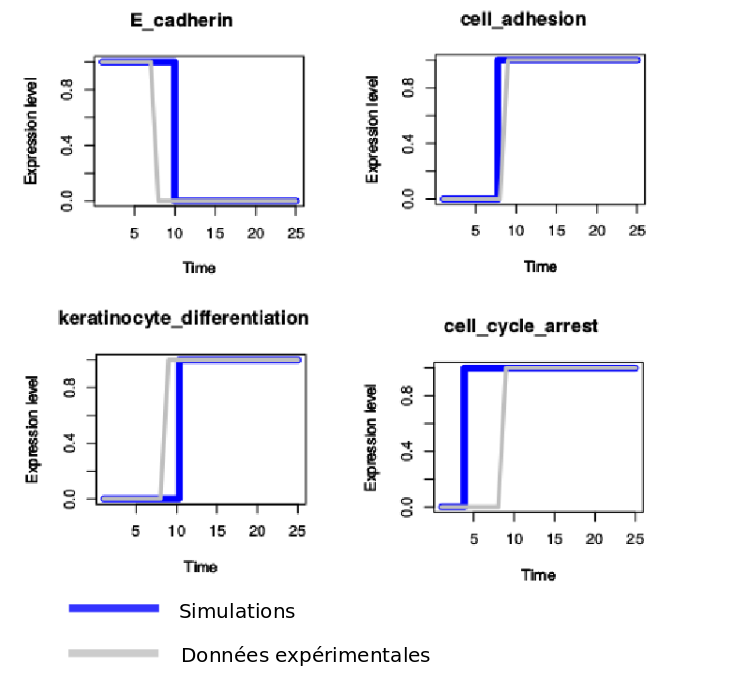
\includegraphics[scale=0.2]{figs/key_nodes2.png}
\end{center}

\textbf{Simulations}

\begin{itemize}
  \item Ecad conforme avec l'expérience et la modélisation.
 \item Dynamique des processus cellulaire conforme avec la littérature.\\
 {\tiny \color{darkgreen} [\citekolly]},
 {\tiny \color{darkgreen} [\citetu]}
  
\end{itemize}

%\textcolor{couleurtheme}{$\Rightarrow$} \fbox{\tval{\large Analyse???}} \textcolor{couleurtheme}{$\Leftarrow$}

\end{frame}




\begin{frame}[c]
  \frametitle{Simulations et analyses}
  \framesubtitle{Simulations des gènes}
  
 \begin{center}
  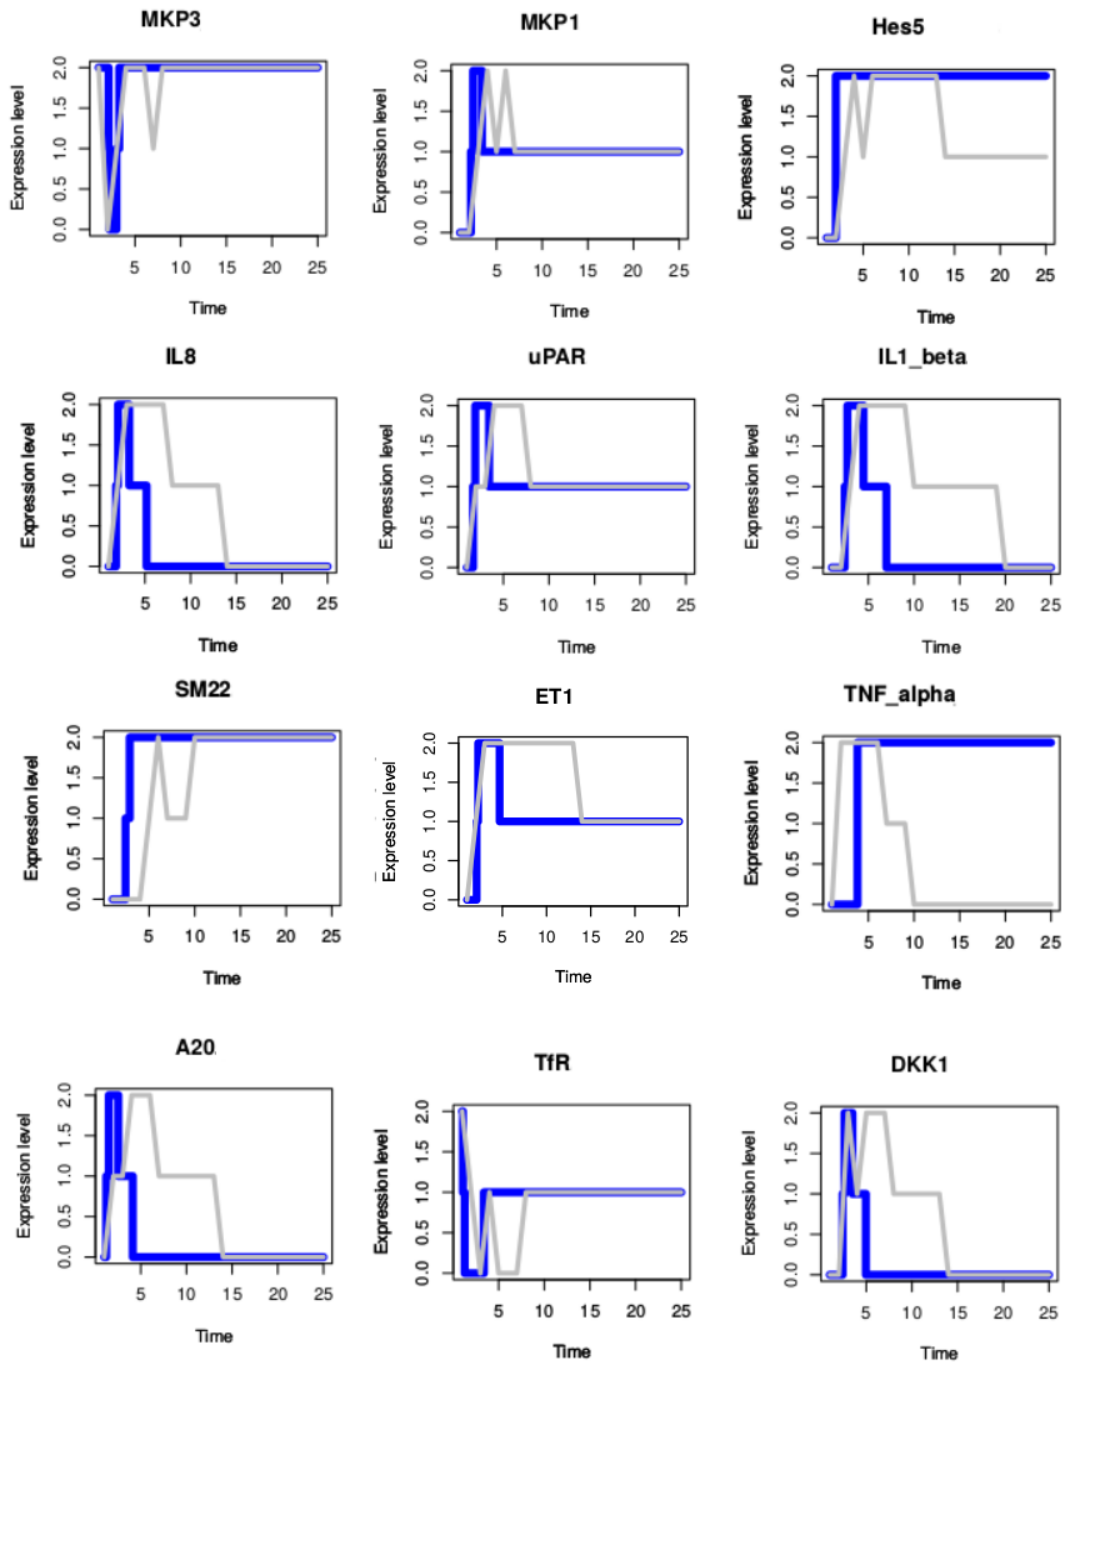
\includegraphics[scale=0.15]{figs/12genes_sim.png}
\end{center}

\textbf{Simulations}

\begin{itemize}
  \item Protéines de signalisation:  $r_{a} = r_{i}=10.0$ et $sa = 50 $.
  \item Estimation de  $r$ et $sa$ pour les gènes selon leur profil d'expression. 
  
\end{itemize}

%\textcolor{couleurtheme}{$\Rightarrow$} \fbox{\tval{\large Analyse???}} \textcolor{couleurtheme}{$\Leftarrow$}

\end{frame}





 %synchronisation
 %resultat de la synchronisation
  
 \subsection{Analyse statistique des traces}
  \begin{frame}
   \frametitle{Simulation et analyse statistique des traces des simulations}
   %\framesubtitle{work with Guillaume Taupiac}


\begin{columns}
\begin{column}{0.5\textwidth}

\scalebox{0.9}{
\begin{tikzpicture}[scale = 0.8]
       
    \draw[thick, ->] (-.2,-.1)--(7,-.1) node[below]{$t$};
     \foreach \t in {1,2,3,4,5,6}
      \draw[very thick] (\t,-1pt)--(\t,-2pt) node[below,blue]{\small\t};

     \draw[thick, ->] (0,-.2)--(0,3) node[left]{$Niveau$};
     \foreach \y in {0,1,2}
      \draw[very thick] (2pt,\y)--(-2pt,\y) node[left,blue]{\small\y};
    
    
    \draw[thick,dotted,blue] (0,0) -- (2,0) node[below]{}; 
    \draw[thick,dotted,blue] (2,0) -- (2,1) node[below]{}; 
    \draw[thick,dotted,blue] (2,1) -- (4,1) node[below]{};
    \draw[thick,dotted,blue] (4,1) -- (4,0) node[below]{};
    \draw[thick,dotted,blue] (4,0) -- (6,0) node[below]{};
    \node[instruct,align=center] (mot2) at (4,2) {$\omega=010$};

\end{tikzpicture}
}


%deuxième exemple 
\scalebox{0.9}{
\begin{tikzpicture}[scale = 0.8]
       
    \draw[thick, ->] (-.2,-.1)--(7,-.1) node[below]{$t$};
     \foreach \t in {1,2,3,4,5,6}
      \draw[very thick] (\t,-1pt)--(\t,-2pt) node[below,blue]{\small \t};

     \draw[thick, ->] (0,-.2)--(0,3) node[left]{$Niveau$};
     \foreach \y in {0,1,2}
      \draw[very thick] (2pt,\y)--(-2pt,\y) node[left,blue]{\small \y};
    
    
    \draw[thick,dotted,blue] (0,0) -- (1,0) node[below]{}; 
    \draw[thick,dotted,blue] (1,0) -- (1,1) node[below]{}; 
    \draw[thick,dotted,blue] (1,1) -- (2,1) node[below]{};
    \draw[thick,dotted,blue] (2,1) -- (2,2) node[below]{};
    \draw[thick,dotted,blue] (2,2) -- (3,2) node[below]{};
    \draw[thick,dotted,blue] (3,2) -- (3,1) node[below]{};
    \draw[thick,dotted,blue] (3,1) -- (5,1) node[below]{};
    \draw[thick,dotted,blue] (5,1) -- (5,0) node[below]{};
    \draw[thick,dotted,blue] (5,0) -- (6,0) node[below]{};
    \node[instruct,align=center] (mot2) at (5,2) {$\omega=01210$};
   

\end{tikzpicture}
}


\end{column}


\begin{column}{0.5\textwidth}

Pour chaque composant \tval{$C_{i}$, $1 \leq i \leq P$},
\tval{$N$} simulations génèrent \tval{$\omega_{i1}, \omega_{i2}, \ldots ,\omega_{iN}$} mots.




Pour $1 \leq j \leq N$

%\newline
%\vspace{1cm}



\scalebox{0.9}{
\begin{tikzpicture}[scale = 0.8]
    
    \node[align=center,blue] (mot) at (2,3) {$\omega_{ij} \Rightarrow $};
    
    \draw[blue] (3,2) rectangle (7,4);

    \node[align=center] (automaton) at (5,3) {$\mathcal{A}_{C_{i}}$};
    
    \node[align=center] (accept) at (8,3) {$\Rightarrow \tval{oui}/\alert{non} $};
    
    \node[align=center] (percent) at (5,1) {\tval{$\% Validation = \frac{\card{oui}}{\card{Simulations}}$}};
   

\end{tikzpicture}
}



\end{column}
\end{columns}
\end{frame}
 
\begin{frame}
\frametitle{Simulation et analyse statistique des traces des simulations}
\begin{tabular}{|c|c||c|c|}
\hline

\textbf{Automate} & \textbf{composant} & \textbf{$\%$  validation} & \textbf{$\%$ validation $T_{1}$}
\\ \hline

$\mathcal{A}_{2}(01210)$ & A20 & 91 & 100 
\\ \hline

$\mathcal{A}_{2}(01210)$ & IL1$\_$beta & 81 & 100
\\ \hline

$\mathcal{A}_{2}(01210)$ & IL8 & 93 & 100 
\\ \hline

$\mathcal{A}_{2}(01210)$ & TNF$\_$alpha & 0 & 0
\\ \hline

$\mathcal{A}_{3}(0121)$ & uPar & 76 & 99 
\\ \hline

$\mathcal{A}_{3}(0121)$ & ET1 & 8 & 19 
\\ \hline

$\mathcal{A}_{4}(0121210)$ & DKK1 & 13 & 43

\\ \hline

$\mathcal{A}_{5}(012121)$ & Hes5 & 0 & 17 
\\ \hline

$\mathcal{A}_{5}(012121)$ & MKP1 & 9 & 97
\\ \hline

$\mathcal{A}_{6}(0212)$ & SM22 & 11 & 100 
\\ \hline

$\mathcal{A}_{7}(02010)$ & MKP3 & 11 & 98

\\ \hline

$\mathcal{A}_{8}(02121)$ & Tfr & 0 & 94 
\\ \hline

\end{tabular}

\medskip

\textbf{Nombre de simulation: 100}\\
\textbf{$T_1$: Tolérance de type $T_1$.}

\end{frame}



\begin{comment}
\begin{frame}
   \frametitle{Simulation and Trace analysis}
   %\framesubtitle{work with Guillaume Taupiac}


\begin{columns}
\begin{column}{0.5\textwidth}

\scalebox{0.9}{
\begin{tikzpicture}[scale = 0.8]
       
    \draw[thick, ->] (-.2,-.1)--(7,-.1) node[below]{$t$};
     \foreach \t in {1,2,3,4,5,6}
      \draw[very thick] (\t,-1pt)--(\t,-2pt) node[below,blue]{\small\t};

     \draw[thick, ->] (0,-.2)--(0,3) node[left]{$Level$};
     \foreach \y in {0,1,2}
      \draw[very thick] (2pt,\y)--(-2pt,\y) node[left,blue]{\small\y};
    
    
    \draw[thick,dotted,blue] (0,0) -- (2,0) node[below]{}; 
    \draw[thick,dotted,blue] (2,0) -- (2,1) node[below]{}; 
    \draw[thick,dotted,blue] (2,1) -- (4,1) node[below]{};
    \draw[thick,dotted,blue] (4,1) -- (4,0) node[below]{};
    \draw[thick,dotted,blue] (4,0) -- (6,0) node[below]{};
    \node[instruct,align=center] (mot2) at (4,2) {$w=010$};

\end{tikzpicture}
}


%deuxième exemple 
\scalebox{0.9}{
\begin{tikzpicture}[scale = 0.8]
       
    \draw[thick, ->] (-.2,-.1)--(7,-.1) node[below]{$t$};
     \foreach \t in {1,2,3,4,5,6}
      \draw[very thick] (\t,-1pt)--(\t,-2pt) node[below,blue]{\small \t};

     \draw[thick, ->] (0,-.2)--(0,3) node[left]{$Level$};
     \foreach \y in {0,1,2}
      \draw[very thick] (2pt,\y)--(-2pt,\y) node[left,blue]{\small \y};
    
    
    \draw[thick,dotted,blue] (0,0) -- (1,0) node[below]{}; 
    \draw[thick,dotted,blue] (1,0) -- (1,1) node[below]{}; 
    \draw[thick,dotted,blue] (1,1) -- (2,1) node[below]{};
    \draw[thick,dotted,blue] (2,1) -- (2,2) node[below]{};
    \draw[thick,dotted,blue] (2,2) -- (3,2) node[below]{};
    \draw[thick,dotted,blue] (3,2) -- (3,1) node[below]{};
    \draw[thick,dotted,blue] (3,1) -- (5,1) node[below]{};
    \draw[thick,dotted,blue] (5,1) -- (5,0) node[below]{};
    \draw[thick,dotted,blue] (5,0) -- (6,0) node[below]{};
    \node[instruct,align=center] (mot2) at (5,2) {$w=01210$};
   

\end{tikzpicture}
}


\end{column}


\begin{column}{0.5\textwidth}

\begin{tabular}{|c|c||c|c|}
\hline

\textbf{Automate}

&

\textbf{components}

&

\textbf{$\%$  validation}

&

\textbf{$\%$ of acceptance $T_{1}$}
\\ \hline

$\mathcal{A}_{2}(01210)$

&

A20

&

91

&

100
\\ \hline

$\mathcal{A}_{2}(01210)$

&

IL1$\_$beta

&

81

&

100
\\ \hline

$\mathcal{A}_{2}(01210)$

&

IL8

&

93

&

100

\\ \hline

$\mathcal{A}_{2}(01210)$

&

TNF$\_$alpha

&

0

&

0

\\ \hline

$\mathcal{A}_{3}(01211)$

&

uPar

&

76

&

99

\\ \hline

$\mathcal{A}_{3}(01211)$

&

ET1

&

8

&

19

\\ \hline

$\mathcal{A}_{4}(0121210)$

&

DKK1

&

13

&

43

\\ \hline

$\mathcal{A}_{5}(0121211)$

&

Hes5


&

0

&

17

\\ \hline

$\mathcal{A}_{5}(0121211)$

&

MKP1


&

9

&

97

\\ \hline

$\mathcal{A}_{6}(0212)$

&

SM22


&

11

&

100

\\ \hline

$\mathcal{A}_{7}(02010)$

&

MKP3


&

11

&

98

\\ \hline

$\mathcal{A}_{8}(02121)$

&

Tfr


&

0

&

94

\\ \hline

 
\end{tabular}


\end{column}
\end{columns}
\end{frame}
\end{comment}

\begin{frame}[c]
  \frametitle{Synthèse sur l'intégration des données}

%mots clés: large scale
%bien expliquer les résultats obtenus
% \textbf{Summary}

%\pause
\tval{Modélisation hybride des réseaux RSTC}\\
\medskip
\textbf{Formalisation des connaissances biologiques}
  \begin{itemize}
   \item Identification des motifs minimaux dans les RSTC. 
   \item Raffinement structurel de la dynamique avec des automates de synchronisation.
  \end{itemize}
\medskip
\textbf{Intégration des paramètres temporels et stochastiques \& simulation}
\begin{itemize}
 \item Inférence des paramètres des données de séries temporelles.
 \item Simulation stochastique sur des modèles biologiques réels.
 \item Analyse statistique des traces des simulations.
\end{itemize}
\medskip
\textbf{Publication}
\begin{itemize}
 \footnotesize
 \item
Louis Fippo Fitime, Christian Schuster, Peter Angel, Olivier Roux, Carito Guziolowski. \tscite{Integrating time-series data in large-scale discrete
cell-based models}. In A. Abate and D. Safranek, editors, \textit{4th International Workshop on Hybrid Systems
Biology (HSB'2015)}, Lecture Notes in Computer Science. September 2015.

\end{itemize}

\end{frame}


% %mettre une transition


\section{Analyse statique des propriétés quantitatives dans les réseaux d'automates stochastiques}
\begin{frame}[c]
 \frametitle{Contributions}
 
 \begin{tikzpicture}[auto]
 
 \draw[thick, ->] (-3.5,0)--node[near end,above,rotate=90] {\scriptsize Niveau d'abstraction des dynamiques}(-3.5,8);
 
 \node[debutfin,align=center] (niv1) at (-2,7) {\begin{tikzpicture}[auto,scale=0.5] 
                                                 \path[use as bounding box] (-0.7,-0.3) rectangle (2.5,2);

                                                              \node[qgre,scale=0.5] (a) at (0,2) {a};
                                                              \node[mod,scale=0.5] (i) at (1,1) {i};
                                                              \node[qgre,scale=0.5] (b) at (0,0) {b};
                                                              \node[qgre,scale=0.5] (c) at (2,1) {c};
                                                              \path
                                                                (a) edge[inh,scale=0.1] (i)
                                                                (b) edge[act,scale=0.1] (i)
                                                                (i) edge[st,scale=0.1]  (c);
                                                              
                                                 \end{tikzpicture}};
                                                 
 \node[debutfin,align=center] (niv2) at (-2,4) {\begin{tikzpicture}[auto,scale=0.5] 
                                                 \path[use as bounding box] (-0.7,-0.3) rectangle (2.5,2);

                                                              \node[qgre,scale=0.5] (a) at (0,2) {a};
                                                              \node[mod,scale=0.5] (i) at (1,1) {i};
                                                              \node[qgre,scale=0.5] (b) at (0,0) {b};
                                                              \node[qgre,scale=0.5] (c) at (2,1) {c};
                                                              \path
                                                                (a) edge[inh,scale=0.1] (i)
                                                                (b) edge[act,scale=0.1] (i)
                                                                (i) edge[st,scale=0.1]  (c);
                                                                
                                                  \node[grandplus] (plus) at (1.2,0.2) {$+$};
                                                  \node[grandplus] (plus) at (2,0) {$K$};
                                                              
                                                 \end{tikzpicture}};
                                                
 \node[debutfin,align=center] (niv3) at (-2,1) {\begin{tikzpicture}[auto,scale=0.5] 
                                                 \path[use as bounding box] (-0.7,-0.3) rectangle (2.5,2);

                                                              \node[qgre,scale=0.5] (a) at (0,2) {a};
                                                              \node[mod,scale=0.5] (i) at (1,1) {i};
                                                              \node[qgre,scale=0.5] (b) at (0,0) {b};
                                                              \node[qgre,scale=0.5] (c) at (2,1) {c};
                                                              \path
                                                                (a) edge[inh,scale=0.1] (i)
                                                                (b) edge[act,scale=0.1] (i)
                                                                (i) edge[st,scale=0.1]  (c);
                                                                
                                                  \node[grandplus] (plus) at (1,0) {$+$};
                                                  \node[grandplus] (plus) at (2,0.5) {$K$};
                                                  \node[scale=0.5] (clock) at (2,-0.25) {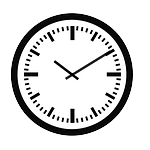
\includegraphics[scale=0.22]{figs/clock.png}};
                                                              
                                                 \end{tikzpicture}};
                                                 

 
 %\node[grandplus] (plus) at (2,0) {$+$};
 

 
 \draw[thick, ->] (7.8,8)--node[near end,below,rotate=90] {\scriptsize Précision des propriétés}(7.8,0); %ligne de la précision des propriétés 
 
 
 
 
 % liste des propriétés
 %general properties
 \node[instruct,align=center] (gp) at (5.8,7) {\begin{tabular}{c}
                                            {\scriptsize Propriétés générales: bornes} \\ 
                                            {\scriptsize sur le nbr d'attracteurs;}\\ {\scriptsize fonctionnalités,...}
                                           \end{tabular}};
 
 %fixed points
 \node[instruct,align=center] (fp) at (6.7,5.6) {\begin{tabular}{c}
                                                 {\scriptsize \'Etats stables}
                                                 \end{tabular}};
                                           
 %reachabilities
 \node[instruct,align=center] (reach) at (6.7,4) {\begin{tabular}{c} {\scriptsize Bifurcations} \\ {\scriptsize Accessibilité} \\ {\scriptsize (CTL)} \end{tabular}};
 \node[instruct,align=center] (qreach) at (6.7,1) {\begin{tabular}{c} {\scriptsize Accessibilité} \\ {\scriptsize quantitative} \\{\scriptsize (CCSL)} \end{tabular}};
 
 
 %process hitting
 

 
 
 
 \uncover<1->{
 
% \begin{pgfonlayer}{background}
 \draw[->,color=gray!10,bend right,line width=4pt,round] (niv3)--node[near center,below] {\scriptsize }(qreach);
 
 \draw[->,color=gray!10,bend right,line width=0.5pt] (niv1)-- (gp);
 
  \draw[->,color=gray!10,bend right,line width=0.6pt,round] (niv2)--node[near center,below] {\scriptsize }(fp);
 
 \draw[->,color=gray!10,bend right,line width=2pt,round] (niv2)--node[near center,below] {\scriptsize }(reach);
% \end{pgfonlayer}
 
   
 %ajout de la notion de chronométrie
 \draw[gray!80,loosely dashed] (-4,2.5) -- node[very near start,below] {\scriptsize Chronométrie}node[very near start,above] {\scriptsize Chronologie}node[very near end,below] {\scriptsize Quantitative}node[very near end,above] {\scriptsize Qualitative}(8,2.5);

 
 }
 
 \uncover<1->{
 \node[es,align=center] (ph) at (2,4.5) {\begin{tabular}{c}
                                           {\scriptsize \textbf{Réseaux} }\\ 
                                           {\scriptsize \textbf{d'automates}}
                                           \end{tabular}};
 \node[instruct,align=center] (pint) at (2,3) {\scriptsize PINT};
 \draw[->,dashed] (ph)--(pint);
 }
 
 
 %les relations
 \uncover<1->{
 \draw[suite,color=gray] (niv1)--(ph);
 \draw[suite,color=gray] (niv2)--(ph);
  \draw[suite,line width=0.5pt,color=gray] (ph)--node[near center,above,rotate=18] {\scriptsize Analyse statique}(fp);
 \draw[suite,color=darkblue,line width=2pt] (niv3)--node[near center,above,bend right,rotate=45] {\scriptsize Modélisation}node[inner,below]{1}(ph);
 \draw[suite,darkblue,round,line width=2pt]     (pint) --node[near center,above,bend right,rotate=90] {\scriptsize Simulation}node[inner,right]{2}(2,1.5)-- node[near center,above,bend right] {\scriptsize Analyse} (niv3);
 \draw[suite,color=blue!60] (ph)--node[near center,above,rotate=-35] {\scriptsize Analyse statique}node[inner,below]{3}(qreach);
  \draw[suite,blue!60] (ph)--node[near center,above,blue!60,rotate=-5] {\scriptsize Analyse statique}node[inner,below]{4}(reach);
 }
 
 \uncover<2->{
  %\draw[suite,color=darkblue] (niv3)--node[near center,above,bend right,rotate=45] {\scriptsize Modélisation}node[inner,below]{1}(ph);
  %\draw[suite,darkblue,round]     (pint) --node[near center,above,bend right,rotate=90] {\scriptsize Simulation}node[inner,right]{2}(2,1.5)-- node[near center,above,bend right] {\scriptsize Analyse} (niv3);
  \draw[suite,color=darkblue,line width=2pt] (ph)--node[near center,above,rotate=-35] {\scriptsize Analyse statique}node[inner,below]{3}(qreach);
 }
 
  
 \end{tikzpicture}

 
\end{frame}

 
\begin{frame}
\frametitle{SAN abstraits comme CTMC}
\begin{columns}
 \begin{column}{0.5\textwidth}
 \begin{figure}[p]
\centering
\scalebox{0.25}{

\begin{tikzpicture}[line join=bevel,font=\LARGE]
%%
  \node (6) at (405.0bp,18.0bp) [reach] {$\langle \mathbf{\color{blue}a_2},b_1,c_0\rangle$};
  \node (2) at (405.0bp,90.0bp) [reach] {$\langle \mathbf{\color{blue}a_2},b_0,c_0\rangle$};

\node (1) at (570.0bp,90.0bp) [reach] {$\langle a_1,b_0,c_0\rangle$};
  \node (64) at (304.0bp,234.0bp) [reach] {$\langle a_0,b_0,c_1\rangle$};
  \node (0) at (469.0bp,162.0bp) [reach] {$\langle a_0,b_0,c_0\rangle}$};
  \node (5) at (507.0bp,306.0bp) [reach] {$\langle a_1,b_1,c_0\rangle$};
  \node (4) at (469.0bp,234.0bp) [reach] {$\langle a_0,b_1,c_0\rangle$};
  \node (69) at (425.0bp,378.0bp) [reach] {$\mathbf{\color{Maroon}s =\langle a_1,b_1,c_1\rangle$};
  \node (68) at (342.0bp,306.0bp) [reach] {$\langle a_0,b_1,c_1\rangle$};
  \node (65) at (232.0bp,450.0bp) [reach] {$\langle a_1,b_0,c_1\rangle$};

  \node[elipse,fill=gray!30] (129) at (88.0bp,90.0bp)  {$\langle a_1,b_0,c_2\rangle$};
  \node[elipse,fill=gray!30] (128) at (139.0bp,162.0bp)  {$\langle a_0,b_0,c_2\rangle$};
  \node[elipse,fill=gray!30] (133) at (112.0bp,306.0bp)  {$\langle a_1,b_1,c_2\rangle$};
  \node[elipse,fill=gray!30] (132) at (139.0bp,234.0bp)  {$\langle a_0,b_1,c_2\rangle$};

  \draw [->] (0) ..controls (445.65bp,135.46bp) and (435.95bp,124.86bp)  .. node[auto] {$\mathbf{\color{Maroon} 2}$}(2);
  \draw [->] (133) ..controls (121.57bp,280.18bp) and (125.26bp,270.62bp)  .. node[auto] {$\mathbf{\color{Maroon} 1}$}(132);
  \draw [->] (65) ..controls (104.12bp,424.19bp) and (0.0bp,387.99bp)  ..  (0.0bp,307.0bp) .. controls (0.0bp,307.0bp) and (0.0bp,307.0bp)  ..  node[auto] {$\mathbf{\color{Maroon} 2}$} (0.0bp,233.0bp) .. controls (0.0bp,185.75bp) and (35.64bp,141.13bp)  .. node[auto] {$\mathbf{\color{Maroon} 3}$}(129);
  \draw [->] (65) ..controls (223.97bp,401.24bp) and (228.52bp,336.68bp)  .. (251.0bp,288.0bp) .. controls (255.96bp,277.25bp) and (263.67bp,266.89bp)  .. node[auto] {$\mathbf{\color{Maroon} 1}$}(64);
  \draw [->] (5) ..controls (483.32bp,333.07bp) and (470.02bp,344.55bp)  .. node[auto] {$\mathbf{\color{Maroon} 2}$}(69);
  \draw [->] (64) ..controls (244.15bp,207.61bp) and (210.57bp,193.36bp)  .. node[auto] {$\mathbf{\color{Maroon} 2}$} (128);
  \draw [->] (5) ..controls (493.43bp,280.01bp) and (488.11bp,270.2bp)  .. node[auto] {$\mathbf{\color{Maroon} 1}$}(4);
  \draw [->] (0) ..controls (475.71bp,188.03bp) and (475.94bp,197.36bp)  .. node[right] {$\mathbf{\color{Maroon} 3}$}(4);
  \draw [->] (1) ..controls (588.79bp,134.38bp) and (608.0bp,186.55bp)  .. (608.0bp,233.0bp) .. controls (608.0bp,307.0bp) and (608.0bp,307.0bp)  .. (608.0bp,307.0bp) .. controls (608.0bp,366.83bp) and (560.73bp,369.68bp)  .. (507.0bp,396.0bp) .. controls (446.14bp,425.81bp) and (370.03bp,438.87bp)  .. node[auto] {$\mathbf{\color{Maroon} 3}$}(65);
  \draw [->] (1) ..controls (572.33bp,138.66bp) and (571.97bp,203.11bp)  .. (551.0bp,252.0bp) .. controls (546.57bp,262.33bp) and (539.46bp,272.21bp)  .. node[right] {$\mathbf{\color{Maroon} 3}$}(5);
  \draw [->] (129) ..controls (68.077bp,117.99bp) and (60.513bp,131.04bp)  .. (57.0bp,144.0bp) .. controls (44.446bp,190.33bp) and (38.221bp,207.83bp)  .. (57.0bp,252.0bp) .. controls (61.945bp,263.63bp) and (70.831bp,273.95bp)  .. node[auto] {$\mathbf{\color{Maroon} 3}$}(133);
  \draw [->] (128) ..controls (145.71bp,188.03bp) and (145.94bp,197.36bp)  .. node[right] {$\mathbf{\color{Maroon} 3}$}(132);
  \draw [->] (69) ..controls (448.8bp,350.83bp) and (462.16bp,339.29bp)  .. node[auto] {$\mathbf{\color{Maroon} 3}$}(5);
  \draw [->] (2) ..controls (405.0bp,63.983bp) and (405.0bp,54.712bp)  .. node[auto] {$\mathbf{\color{Maroon} 3}$}(6);
  \draw [->] (0) ..controls (499.93bp,134.79bp) and (517.41bp,122.58bp)  .. node[auto] {$\mathbf{\color{Maroon} 1}$}(1);
  \draw [->] (68) ..controls (388.56bp,279.34bp) and (412.1bp,266.36bp)  .. node[auto] {$\mathbf{\color{Maroon} 1}$}(4);
  \draw [->] (68) ..controls (321.75bp,280.09bp) and (316.27bp,270.41bp)  .. node[auto] {$\mathbf{\color{Maroon} 3}$}(64);
  \draw [->] (1) ..controls (539.0bp,117.26bp) and (521.52bp,129.47bp)  .. node[auto] {$\mathbf{\color{Maroon} 2}$}(0);
  \draw [->] (65) ..controls (301.71bp,423.72bp) and (343.47bp,408.57bp)  .. node[auto] {$\mathbf{\color{Maroon} 3}$}(69);
  \draw [->] (64) ..controls (324.32bp,260.04bp) and (329.77bp,269.67bp)  .. node[auto] {$\mathbf{\color{Maroon} 1}$}(68);
  \draw [->] (69) ..controls (394.58bp,351.34bp) and (381.1bp,339.97bp)  .. node[auto] {$\mathbf{\color{Maroon} 1}$}(68);
  \draw [->] (128) ..controls (114.09bp,136.08bp) and (106.38bp,125.8bp)  .. node[auto] {$\mathbf{\color{Maroon} 1}$}(129);
  \draw [->] (64) ..controls (285.73bp,261.68bp) and (275.22bp,274.54bp)  .. (269.0bp,288.0bp) .. controls (248.81bp,331.74bp) and (243.08bp,388.29bp)  .. node[auto] {$\mathbf{\color{Maroon} 2}$}(65);
  \draw [->] (132) ..controls (132.3bp,208.35bp) and (132.06bp,199.03bp)  .. node[auto] {$\mathbf{\color{Maroon} 1}$}(128);
  \draw [->] (4) ..controls (462.3bp,208.35bp) and (462.06bp,199.03bp)  .. node[left] {$\mathbf{\color{Maroon} 1}$}(0);
  \draw [->] (129) ..controls (113.05bp,116.11bp) and (120.71bp,126.32bp)  .. node[auto] {$\mathbf{\color{Maroon} 2}$}(128);
%
\end{tikzpicture}


}

\label{ex-bifurcations}
\end{figure}
Inconvénient: \textcolor{red}{explosion de l'espace d'états.}
  
 \end{column}
 
 \begin{column}{0.5\textwidth}
  \textbf{La probabilité d'effectuer une transition depuis l'état s:}
  $$\ppexit{s}{*}{t} = 1-e^{-\lambda t}$$ \\
  \medskip
  \textbf{Probabilité d'effectuer une transition de s à s':}
  $$\ppexit{s}{s^{'}}{t} = \frac{R (s,s^{'})}{E (s)} \cdot \ppexit{s}{*}{t}$$\\
  \medskip
  \textbf{Probabilité d'effectuer une transition de s à un ensemble d'états:}
  $$\ppexit{s}{A}{t} = \frac{R (s,A)}{E (s)} \cdot \ppexit{s}{*}{t}$$ \\
 \end{column}

\end{columns}

\end{frame}

\begin{frame}
\frametitle{SAN abstraits comme CTMC}
\begin{figure}[p]
\centering
\scalebox{0.4}{

\begin{tikzpicture}[line join=bevel,font=\LARGE]
%%
  \node (6) at (405.0bp,18.0bp) [reach] {$\langle \mathbf{\color{blue}a_2},b_1,c_0\rangle$};
  \node (2) at (405.0bp,90.0bp) [reach] {$\langle \mathbf{\color{blue}a_2},b_0,c_0\rangle$};

\node (1) at (570.0bp,90.0bp) [reach] {$\langle a_1,b_0,c_0\rangle$};
  \node (64) at (304.0bp,234.0bp) [reach] {$\langle a_0,b_0,c_1\rangle$};
  \node (0) at (469.0bp,162.0bp) [reach] {$\langle a_0,b_0,c_0\rangle}$};
  \node (5) at (507.0bp,306.0bp) [reach] {$\langle a_1,b_1,c_0\rangle$};
  \node (4) at (469.0bp,234.0bp) [reach] {$\langle a_0,b_1,c_0\rangle$};
  \node (69) at (425.0bp,378.0bp) [reach] {$\mathbf{\color{Maroon}s =\langle a_1,b_1,c_1\rangle$};
  \node (68) at (342.0bp,306.0bp) [reach] {$\langle a_0,b_1,c_1\rangle$};
  \node (65) at (232.0bp,450.0bp) [reach] {$\langle a_1,b_0,c_1\rangle$};

  \node[elipse,fill=gray!30] (129) at (88.0bp,90.0bp)  {$\langle a_1,b_0,c_2\rangle$};
  \node[elipse,fill=gray!30] (128) at (139.0bp,162.0bp)  {$\langle a_0,b_0,c_2\rangle$};
  \node[elipse,fill=gray!30] (133) at (112.0bp,306.0bp)  {$\langle a_1,b_1,c_2\rangle$};
  \node[elipse,fill=gray!30] (132) at (139.0bp,234.0bp)  {$\langle a_0,b_1,c_2\rangle$};

  \draw [->] (0) ..controls (445.65bp,135.46bp) and (435.95bp,124.86bp)  .. node[auto] {$\mathbf{\color{Maroon} 2}$}(2);
  \draw [->] (133) ..controls (121.57bp,280.18bp) and (125.26bp,270.62bp)  .. node[auto] {$\mathbf{\color{Maroon} 1}$}(132);
  \draw [->] (65) ..controls (104.12bp,424.19bp) and (0.0bp,387.99bp)  ..  (0.0bp,307.0bp) .. controls (0.0bp,307.0bp) and (0.0bp,307.0bp)  ..  node[auto] {$\mathbf{\color{Maroon} 2}$} (0.0bp,233.0bp) .. controls (0.0bp,185.75bp) and (35.64bp,141.13bp)  .. node[auto] {$\mathbf{\color{Maroon} 3}$}(129);
  \draw [->] (65) ..controls (223.97bp,401.24bp) and (228.52bp,336.68bp)  .. (251.0bp,288.0bp) .. controls (255.96bp,277.25bp) and (263.67bp,266.89bp)  .. node[auto] {$\mathbf{\color{Maroon} 1}$}(64);
  \draw [->] (5) ..controls (483.32bp,333.07bp) and (470.02bp,344.55bp)  .. node[auto] {$\mathbf{\color{Maroon} 2}$}(69);
  \draw [->] (64) ..controls (244.15bp,207.61bp) and (210.57bp,193.36bp)  .. node[auto] {$\mathbf{\color{Maroon} 2}$} (128);
  \draw [->] (5) ..controls (493.43bp,280.01bp) and (488.11bp,270.2bp)  .. node[auto] {$\mathbf{\color{Maroon} 1}$}(4);
  \draw [->] (0) ..controls (475.71bp,188.03bp) and (475.94bp,197.36bp)  .. node[right] {$\mathbf{\color{Maroon} 3}$}(4);
  \draw [->] (1) ..controls (588.79bp,134.38bp) and (608.0bp,186.55bp)  .. (608.0bp,233.0bp) .. controls (608.0bp,307.0bp) and (608.0bp,307.0bp)  .. (608.0bp,307.0bp) .. controls (608.0bp,366.83bp) and (560.73bp,369.68bp)  .. (507.0bp,396.0bp) .. controls (446.14bp,425.81bp) and (370.03bp,438.87bp)  .. node[auto] {$\mathbf{\color{Maroon} 3}$}(65);
  \draw [->] (1) ..controls (572.33bp,138.66bp) and (571.97bp,203.11bp)  .. (551.0bp,252.0bp) .. controls (546.57bp,262.33bp) and (539.46bp,272.21bp)  .. node[right] {$\mathbf{\color{Maroon} 3}$}(5);
  \draw [->] (129) ..controls (68.077bp,117.99bp) and (60.513bp,131.04bp)  .. (57.0bp,144.0bp) .. controls (44.446bp,190.33bp) and (38.221bp,207.83bp)  .. (57.0bp,252.0bp) .. controls (61.945bp,263.63bp) and (70.831bp,273.95bp)  .. node[auto] {$\mathbf{\color{Maroon} 3}$}(133);
  \draw [->] (128) ..controls (145.71bp,188.03bp) and (145.94bp,197.36bp)  .. node[right] {$\mathbf{\color{Maroon} 3}$}(132);
  \draw [->] (69) ..controls (448.8bp,350.83bp) and (462.16bp,339.29bp)  .. node[auto] {$\mathbf{\color{Maroon} 3}$}(5);
  \draw [->] (2) ..controls (405.0bp,63.983bp) and (405.0bp,54.712bp)  .. node[auto] {$\mathbf{\color{Maroon} 3}$}(6);
  \draw [->] (0) ..controls (499.93bp,134.79bp) and (517.41bp,122.58bp)  .. node[auto] {$\mathbf{\color{Maroon} 1}$}(1);
  \draw [->] (68) ..controls (388.56bp,279.34bp) and (412.1bp,266.36bp)  .. node[auto] {$\mathbf{\color{Maroon} 1}$}(4);
  \draw [->] (68) ..controls (321.75bp,280.09bp) and (316.27bp,270.41bp)  .. node[auto] {$\mathbf{\color{Maroon} 3}$}(64);
  \draw [->] (1) ..controls (539.0bp,117.26bp) and (521.52bp,129.47bp)  .. node[auto] {$\mathbf{\color{Maroon} 2}$}(0);
  \draw [->] (65) ..controls (301.71bp,423.72bp) and (343.47bp,408.57bp)  .. node[auto] {$\mathbf{\color{Maroon} 3}$}(69);
  \draw [->] (64) ..controls (324.32bp,260.04bp) and (329.77bp,269.67bp)  .. node[auto] {$\mathbf{\color{Maroon} 1}$}(68);
  \draw [->] (69) ..controls (394.58bp,351.34bp) and (381.1bp,339.97bp)  .. node[auto] {$\mathbf{\color{Maroon} 1}$}(68);
  \draw [->] (128) ..controls (114.09bp,136.08bp) and (106.38bp,125.8bp)  .. node[auto] {$\mathbf{\color{Maroon} 1}$}(129);
  \draw [->] (64) ..controls (285.73bp,261.68bp) and (275.22bp,274.54bp)  .. (269.0bp,288.0bp) .. controls (248.81bp,331.74bp) and (243.08bp,388.29bp)  .. node[auto] {$\mathbf{\color{Maroon} 2}$}(65);
  \draw [->] (132) ..controls (132.3bp,208.35bp) and (132.06bp,199.03bp)  .. node[auto] {$\mathbf{\color{Maroon} 1}$}(128);
  \draw [->] (4) ..controls (462.3bp,208.35bp) and (462.06bp,199.03bp)  .. node[left] {$\mathbf{\color{Maroon} 1}$}(0);
  \draw [->] (129) ..controls (113.05bp,116.11bp) and (120.71bp,126.32bp)  .. node[auto] {$\mathbf{\color{Maroon} 2}$}(128);
%
\end{tikzpicture}


}

\label{ex-bifurcations}
\end{figure}
Inconvénient: \textcolor{red}{explosion de l'espace d'états.}
\end{frame}

 \subsection{Interprétation abstraite quantitative des scénarios}
 \begin{frame}
 \frametitle{Contribution}
 
\begin{figure}[h]
\centering
\begin{tikzpicture}[node distance=1.5cm]
\draw (-4, 0) -- (4, 0);
 % Small tickmarks on the x axis
        \foreach \x in {-4,-1.9,...,4} {
            \draw (\x, 0) -- (\x, -0.8pt);
        }
% Labels on the $x$ axis; the llap makes the label center on the
        % number without the minus.
        \foreach \x/\label in {-4/0,-2/{\color{blue}\binf{\Prob{\pacc}}},0/\Prob{\pacc},2/{\color{blue}\bsup{\Prob{\pacc}}},4/1} {
            \node[x tick label] at (\x, -0.5) {$\label$};
            \draw[major tick] (\x, 0) -- (\x, -1.25pt);
        }
\node[axis label] at (4.5,0) {$\scriptstyle \mathcal{P}$};

\end{tikzpicture}
 \end{figure}
 \hspace{5cm}
 
 \textbf{But:}
 \begin{itemize}
  \item Analyse statique des \tval{propriétés quantitatives}.
  %\item Analyse statique de la  \tval{Probabilité} et du  \tval{Délai} d'une propriété d'accessibilité.
  \item Estimer une \tval{borne inférieure et supérieure} de la probabilité et du délai.  
 \end{itemize}
 \textbf{Contribution:}
 $$
\left\{
    \begin{array}{lcl}
        \mbox{QS (Classes d'équivalences d'états)} &\\  %rajouter un signe entre les deux
        \mbox{+} & \Longrightarrow \mbox{\tval{approximation formelle des propriétés}} \\
        \mbox{IA (Interprétation abstraite)} & \mbox{\ \ \ \ \tval{quantitatives}}
    \end{array}
\right.
$$ 
 

\end{frame}


\begin{frame}[t]
\frametitle{Interprétation abstraite}
\framesubtitle{Causalité locale}
\begin{columns}
%l'automate
\begin{column}{0.4\textwidth}
\begin{center}\scalebox{\scaleex}{
\begin{tikzpicture}
\exanaidef
\end{tikzpicture}
}\end{center}
\end{column}
%le glc associé
\begin{column}{0.6\textwidth}

% local-cause($\obj{d_1}{d_2}$) = \{$\trans{d_1}{d_2}{b_1}$, $\trans{d_1}{d_2}{c_2}$\}
% \medskip
% local-cause^\#($\obj{d_1}{d_2}$) = $\{\{b_1\},\{c_2\}\}$ \\

%\hspace*{5em}

\begin{center}\scalebox{\scaleex}{
%\begin{tikzpicture}
\exlcgaidef
%\end{tikzpicture}
}\end{center}

\end{column}
\end{columns}
\end{frame}

\begin{frame}
\frametitle{Interprétation abstraite}
\framesubtitle{Graphe de causalité locale}
\begin{itemize}
 \item \textbf{Contexte initial/état:} \qex{$\PHetat{a_0,b_0,c_1,d_1,e_1,f_0}$}
 \item \textbf{Goal:} état local {\color{blue}$d_2$}
\end{itemize}
\begin{columns}
\begin{column}{0.5\textwidth}
\begin{center}\scalebox{0.6}{
\begin{tikzpicture}
\exanppdef
\TState{1}{a_0,b_0,c_1,d_1,e_1,f_0}
\end{tikzpicture}
}\end{center}
\end{column}
\begin{column}{0.5\textwidth}
\begin{center}\scalebox{0.7}{
\exglcandef
}\end{center}
\end{column}
\end{columns}
\end{frame}

\begin{frame}
\frametitle{Interprétation abstraite}
\framesubtitle{Causalité locale quantifiée  \& Classes d'équivalence d'états}
\begin{columns}
%l'automate
\begin{column}{0.3\textwidth}
\begin{left}\scalebox{\scaleex}{
\begin{tikzpicture}
\exsanaidef
\end{tikzpicture}
}\end{left}
%$$\Probt{\obj{d_1}{d_2}}(t) = \frac{3_{b_1}+2_{c_2}}{3_{b_1}+2_{c_2}+2_{e_1}}$$
\end{column}
%le glc associé
\begin{column}{0.7\textwidth}

% qlocal-cause($\obj{d_1}{d_2}$) = \{$\trans{d_1}{d_2}{b_1,\mathbf{\color{Maroon} 3}}$, $\trans{d_1}{d_2}{c_2,\mathbf{\color{Maroon} 2}},
% {\color{red} \trans{d_1}{d_0}{e_1,\mathbf{\color{red} 2}}}$\}\\
% \medskip
% qlocal-cause^\#($\obj{d_1}{d_2}$) = $\{\{b_1\},\{c_2\},{\color{red}\{e_1\}}\}$ \\


%$$\Probt{\obj{d_1}{d_2}}(t) =\ppexit{A_{d_1}}{A_{d_2}}{t}= \frac{R (A_{d_1},A_{d_2})}{E (A_{d_1})} \cdot \ppexit{A_{d_1}}{*}{t} $$ \\

%$\ppexit{A_{d_1}}{A_{d_2}}{t}$ \\

%\hspace*{1em}
\begin{center}\scalebox{\scaleex}{
%\begin{tikzpicture}
\exqlcgaidef
%\end{tikzpicture}
}\end{center}

\end{column}
\end{columns}
\end{frame}

\begin{frame}
\frametitle{Interprétation abstraite}
\framesubtitle{Causalité locale quantifiée \& Classe d'équivalences d'états}
\begin{columns}
%l'automate
\begin{column}{0.25\textwidth}
\begin{left}\scalebox{\scaleex}{
\begin{tikzpicture}
\exsanaidef
\end{tikzpicture}
}\end{left}
%$$\Probt{\obj{d_1}{d_2}}(t) = \frac{3_{b_1}+2_{c_2}}{3_{b_1}+2_{c_2}+2_{e_1}}$$
\end{column}
%le glc associé
\begin{column}[c]{0.75\textwidth}

% qlocal-cause($\obj{d_1}{d_2}$) = \{$\trans{d_1}{d_2}{b_1,\mathbf{\color{Maroon} 3}}$, $\trans{d_1}{d_2}{c_2,\mathbf{\color{Maroon} 2}},
% {\color{red} \trans{d_1}{d_0}{e_1,\mathbf{\color{red} 2}}}$\}\\
% \medskip
% qlocal-cause^\#($\obj{d_1}{d_2}$) = $\{\{b_1\},\{c_2\},{\color{red}\{e_1\}}\}$ \\
\begin{center}\scalebox{\scaleex}{
%\begin{tikzpicture}
\exqlcgaidef
%\end{tikzpicture}
}\end{center}


%$$\Probt{\obj{d_1}{d_2}}(t) =\ppexit{A_{d_1}}{A_{d_2}}{t}= \frac{R (A_{d_1},A_{d_2})}{E (A_{d_1})} \cdot \ppexit{A_{d_1}}{*}{t} $$ \\

$$\Probt{\obj{d_1}{d_2}}(t) = \frac{3 \cdot \Prob{b_1} + 2 \cdot \Prob{c_2}}{3 \cdot \Prob{b_1} + 2 \cdot \Prob{c_2}+ {\color{red} 2 \cdot \Prob{e_1}}}\cdot \ppexit{A_{d_1}}{*}{t}$$ \\

\textbf{Approximation:} {\color{red} $\Prob{e_1} = 1$}

% \hspace*{1em}
% \begin{center}\scalebox{\scaleex}{
% %\begin{tikzpicture}
% \exqlcgaidef
% %\end{tikzpicture}
% }\end{center}

\end{column}
\end{columns}


\end{frame}

 \subsection{Graphe de Causalité Locale quantifié}
 %\begin{frame}
\frametitle{Graphe de causalité locale quantifié}

 \begin{itemize}
  
%  \item Probabilité d'un  \tval{n{\oe}ud état local}:\\
%  $\GProbLS{\n}{\ctx}{\cwG}{k}$\\
%  \medskip
%  \pause
%  \item Probabilité d'un  \tval{n{\oe}ud objectif}:\\
%  $\GProbObjn{\n}{\ctx}{\cwG}{k}$\\
%  \medskip
%  \pause
%  \item Probabilité d'un  \tval{n{\oe}ud Solution}:\\
%  $\GProbSol{\n}{\ctx}{\cwG}{k}$
%  \end{itemize}
%  \pause
   \begin{center}\scalebox{\scaleex}{
    
    \exqlcggaidef
   
   }\end{center}
   
%  \end{column}
% \end{columns}


\end{frame}

 \subsection{Estimation de la probabilité et des délais}
 \begin{frame}
\frametitle{Approximation de la probabilité d'accessibilité}
\begin{columns}
 \begin{column}{0.2\textwidth}
  \begin{center}\scalebox{0.6}{
\begin{tikzpicture}
\exsanppdef
\end{tikzpicture}
}\end{center}
 \end{column}
 \begin{column}{0.8\textwidth}
 
 \only<1>{
\tikzstyle{labelproba1}=[transparent]
\tikzstyle{labelproba2}=[transparent]
\tikzstyle{labelproba3}=[transparent]
\tikzstyle{labelproba4}=[transparent]
\tikzstyle{labelproba5}=[transparent]
\tikzstyle{labelproba6}=[transparent]
\tikzstyle{labelproba7}=[transparent]
\tikzstyle{labelproba8}=[transparent]
\tikzstyle{labelproba9}=[transparent]
\tikzstyle{labelproba10}=[transparent]
\tikzstyle{labelproba11}=[transparent]
\tikzstyle{labelproba12}=[transparent]
\begin{center}\scalebox{\scaleex}{
    
    \exglcsandef
   
   }\end{center}

}
 
 \only<2>{
\tikzstyle{labelproba1}=[transparent]
\tikzstyle{labelproba2}=[transparent]
\tikzstyle{labelproba3}=[transparent]
\tikzstyle{labelproba4}=[transparent]
\tikzstyle{labelproba5}=[transparent]
\tikzstyle{labelproba6}=[transparent]
\tikzstyle{labelproba7}=[transparent]
\tikzstyle{labelproba8}=[transparent]
\tikzstyle{labelproba9}=[transparent]
\tikzstyle{labelproba10}=[transparent]
\tikzstyle{labelproba11}=[]
\tikzstyle{labelproba12}=[]
\begin{center}\scalebox{\scaleex}{
    
    \exglcsandef
   
   }\end{center}

}

 \only<3>{
\tikzstyle{labelproba1}=[transparent]
\tikzstyle{labelproba2}=[transparent]
\tikzstyle{labelproba3}=[transparent]
\tikzstyle{labelproba4}=[transparent]
\tikzstyle{labelproba5}=[transparent]
\tikzstyle{labelproba6}=[transparent]
\tikzstyle{labelproba7}=[transparent]
\tikzstyle{labelproba8}=[transparent]
\tikzstyle{labelproba9}=[]
\tikzstyle{labelproba10}=[]
\tikzstyle{labelproba11}=[]
\tikzstyle{labelproba12}=[]
\begin{center}\scalebox{\scaleex}{
    
    \exglcsandef
   
   }\end{center}

}

 \only<4>{
\tikzstyle{labelproba1}=[transparent]
\tikzstyle{labelproba2}=[transparent]
\tikzstyle{labelproba3}=[transparent]
\tikzstyle{labelproba4}=[transparent]
\tikzstyle{labelproba5}=[transparent]
\tikzstyle{labelproba6}=[transparent]
\tikzstyle{labelproba7}=[]
\tikzstyle{labelproba8}=[]
\tikzstyle{labelproba9}=[]
\tikzstyle{labelproba10}=[]
\tikzstyle{labelproba11}=[]
\tikzstyle{labelproba12}=[]
\begin{center}\scalebox{\scaleex}{
    
    \exglcsandef
   
   }\end{center}

}

 \only<5>{
\tikzstyle{labelproba1}=[transparent]
\tikzstyle{labelproba2}=[transparent]
\tikzstyle{labelproba3}=[transparent]
\tikzstyle{labelproba4}=[transparent]
\tikzstyle{labelproba5}=[]
\tikzstyle{labelproba6}=[]
\tikzstyle{labelproba7}=[]
\tikzstyle{labelproba8}=[]
\tikzstyle{labelproba9}=[]
\tikzstyle{labelproba10}=[]
\tikzstyle{labelproba11}=[]
\tikzstyle{labelproba12}=[]
\begin{center}\scalebox{\scaleex}{
    
    \exglcsandef
   
   }\end{center}

}

\only<6>{
\tikzstyle{labelproba1}=[transparent]
\tikzstyle{labelproba2}=[transparent]
\tikzstyle{labelproba3}=[]
\tikzstyle{labelproba4}=[]
\tikzstyle{labelproba5}=[]
\tikzstyle{labelproba6}=[]
\tikzstyle{labelproba7}=[]
\tikzstyle{labelproba8}=[]
\tikzstyle{labelproba9}=[]
\tikzstyle{labelproba10}=[]
\tikzstyle{labelproba11}=[]
\tikzstyle{labelproba12}=[]
\begin{center}\scalebox{\scaleex}{
    
    \exglcsandef
   
   }\end{center}

}

\only<7>{
\tikzstyle{labelproba1}=[]
\tikzstyle{labelproba2}=[]
\tikzstyle{labelproba3}=[]
\tikzstyle{labelproba4}=[]
\tikzstyle{labelproba5}=[]
\tikzstyle{labelproba6}=[]
\tikzstyle{labelproba7}=[]
\tikzstyle{labelproba8}=[]
\tikzstyle{labelproba9}=[]
\tikzstyle{labelproba10}=[]
\tikzstyle{labelproba11}=[]
\tikzstyle{labelproba12}=[]
\begin{center}\scalebox{\scaleex}{
    
    \exglcsandef
   
   }\end{center}

}

   
 \end{column}
 \end{columns}

\end{frame}

% \input{partsfr/delay_fr.tex}
% mettre une slide de conclusion
\begin{frame}[c]
  \frametitle{Synthèse sur l'analyse statique des propriétés quantitatives}

%mots clés: large scale
%bien expliquer les résultats obtenus
% \textbf{Summary}

%\pause
\tval{Approximation des propriétés quantitatives}\\
\medskip
\textbf{Interprétation abstraite des scénarios}
  \begin{itemize}
   \item Causalité locale quantitative.
   \item Graphe de causalité locale quantifié.
  \end{itemize}
\medskip
\textbf{Outil d'aide à la décision}
\begin{itemize}
 \item Borne inférieure de la probabilité et des délais.
 \item Choix des scénarios (plus probable, plus rapide,...).
\end{itemize}
\medskip
\textbf{Intérêt:}
\begin{center}
 \begin{tikzpicture}
  \node[esdef] (defverif) at (4,-5) {\begin{tabular}{c} 
  Exprimer les formules comme: quelle est la probabilité d'observer \\
  une protéine donnée  $a$ après avoir observé une protéine $b$?
   \end{tabular}};
 \end{tikzpicture}

\end{center}



\end{frame}


% %mettre une transition

 \section{Analyse statique des bifurcations}
 \begin{frame}[c]
 \frametitle{Contributions}
 
 \begin{tikzpicture}[auto]
 
 \draw[thick, ->] (-3.5,0)--node[near end,above,rotate=90] {\scriptsize Niveau d'abstraction des dynamiques}(-3.5,8);
 
 \node[debutfin,align=center] (niv1) at (-2,7) {\begin{tikzpicture}[auto,scale=0.5] 
                                                 \path[use as bounding box] (-0.7,-0.3) rectangle (2.5,2);

                                                              \node[qgre,scale=0.5] (a) at (0,2) {a};
                                                              \node[mod,scale=0.5] (i) at (1,1) {i};
                                                              \node[qgre,scale=0.5] (b) at (0,0) {b};
                                                              \node[qgre,scale=0.5] (c) at (2,1) {c};
                                                              \path
                                                                (a) edge[inh,scale=0.1] (i)
                                                                (b) edge[act,scale=0.1] (i)
                                                                (i) edge[st,scale=0.1]  (c);
                                                              
                                                 \end{tikzpicture}};
                                                 
 \node[debutfin,align=center] (niv2) at (-2,4) {\begin{tikzpicture}[auto,scale=0.5] 
                                                 \path[use as bounding box] (-0.7,-0.3) rectangle (2.5,2);

                                                              \node[qgre,scale=0.5] (a) at (0,2) {a};
                                                              \node[mod,scale=0.5] (i) at (1,1) {i};
                                                              \node[qgre,scale=0.5] (b) at (0,0) {b};
                                                              \node[qgre,scale=0.5] (c) at (2,1) {c};
                                                              \path
                                                                (a) edge[inh,scale=0.1] (i)
                                                                (b) edge[act,scale=0.1] (i)
                                                                (i) edge[st,scale=0.1]  (c);
                                                                
                                                  \node[grandplus] (plus) at (1.2,0.2) {$+$};
                                                  \node[grandplus] (plus) at (2,0) {$K$};
                                                              
                                                 \end{tikzpicture}};
                                                
 \node[debutfin,align=center] (niv3) at (-2,1) {\begin{tikzpicture}[auto,scale=0.5] 
                                                 \path[use as bounding box] (-0.7,-0.3) rectangle (2.5,2);

                                                              \node[qgre,scale=0.5] (a) at (0,2) {a};
                                                              \node[mod,scale=0.5] (i) at (1,1) {i};
                                                              \node[qgre,scale=0.5] (b) at (0,0) {b};
                                                              \node[qgre,scale=0.5] (c) at (2,1) {c};
                                                              \path
                                                                (a) edge[inh,scale=0.1] (i)
                                                                (b) edge[act,scale=0.1] (i)
                                                                (i) edge[st,scale=0.1]  (c);
                                                                
                                                  \node[grandplus] (plus) at (1,0) {$+$};
                                                  \node[grandplus] (plus) at (2,0.5) {$K$};
                                                  \node[scale=0.5] (clock) at (2,-0.25) {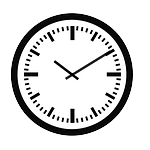
\includegraphics[scale=0.22]{figs/clock.png}};
                                                              
                                                 \end{tikzpicture}};
                                                 

 
 %\node[grandplus] (plus) at (2,0) {$+$};
 

 
 \draw[thick, ->] (7.8,8)--node[near end,below,rotate=90] {\scriptsize Précision des propriétés}(7.8,0); %ligne de la précision des propriétés 
 
 
 
 
 % liste des propriétés
 %general properties
 \node[instruct,align=center] (gp) at (5.8,7) {\begin{tabular}{c}
                                            {\scriptsize Propriétés générales: bornes} \\ 
                                            {\scriptsize sur le nbr d'attracteurs;}\\ {\scriptsize fonctionnalités,...}
                                           \end{tabular}};
 
 %fixed points
 \node[instruct,align=center] (fp) at (6.7,5.6) {\begin{tabular}{c}
                                                 {\scriptsize \'Etats stables}
                                                 \end{tabular}};
                                           
 %reachabilities
 \node[instruct,align=center] (reach) at (6.7,4) {\begin{tabular}{c} {\scriptsize Bifurcations} \\ {\scriptsize Accessibilité} \\ {\scriptsize (CTL)} \end{tabular}};
 \node[instruct,align=center] (qreach) at (6.7,1) {\begin{tabular}{c} {\scriptsize Accessibilité} \\ {\scriptsize quantitative} \\{\scriptsize (CCSL)} \end{tabular}};
 
 
 %process hitting
 

 
 
 
 \uncover<1->{
 
% \begin{pgfonlayer}{background}
 \draw[->,color=gray!10,bend right,line width=4pt,round] (niv3)--node[near center,below] {\scriptsize }(qreach);
 
 \draw[->,color=gray!10,bend right,line width=0.5pt] (niv1)-- (gp);
 
  \draw[->,color=gray!10,bend right,line width=0.6pt,round] (niv2)--node[near center,below] {\scriptsize }(fp);
 
 \draw[->,color=gray!10,bend right,line width=2pt,round] (niv2)--node[near center,below] {\scriptsize }(reach);
% \end{pgfonlayer}
 
   
 %ajout de la notion de chronométrie
 \draw[gray!80,loosely dashed] (-4,2.5) -- node[very near start,below] {\scriptsize Chronométrie}node[very near start,above] {\scriptsize Chronologie}node[very near end,below] {\scriptsize Quantitative}node[very near end,above] {\scriptsize Qualitative}(8,2.5);

 
 }
 
 \uncover<1->{
 \node[es,align=center] (ph) at (2,4.5) {\begin{tabular}{c}
                                           {\scriptsize \textbf{Réseaux} }\\ 
                                           {\scriptsize \textbf{d'automates}}
                                           \end{tabular}};
 \node[instruct,align=center] (pint) at (2,3) {\scriptsize PINT};
 \draw[->,dashed] (ph)--(pint);
 }
 
 
 %les relations
 \uncover<1->{
 \draw[suite,color=gray] (niv1)--(ph);
 \draw[suite,color=gray] (niv2)--(ph);
  \draw[suite,line width=0.5pt,color=gray] (ph)--node[near center,above,rotate=18] {\scriptsize Analyse statique}(fp);
 \draw[suite,color=darkblue,line width=2pt] (niv3)--node[near center,above,bend right,rotate=45] {\scriptsize Modélisation}node[inner,below]{1}(ph);
 \draw[suite,darkblue,round,line width=2pt]     (pint) --node[near center,above,bend right,rotate=90] {\scriptsize Simulation}node[inner,right]{2}(2,1.5)-- node[near center,above,bend right] {\scriptsize Analyse} (niv3);
 \draw[suite,color=darkblue,line width=2pt] (ph)--node[near center,above,rotate=-35] {\scriptsize Analyse statique}node[inner,below]{3}(qreach);
  \draw[suite,blue!60] (ph)--node[near center,above,blue!60,rotate=-5] {\scriptsize Analyse statique}node[inner,below]{4}(reach);
 }
 
 \uncover<2->{
  %\draw[suite,color=darkblue] (niv3)--node[near center,above,bend right,rotate=45] {\scriptsize Modélisation}node[inner,below]{1}(ph);
  %\draw[suite,darkblue,round]     (pint) --node[near center,above,bend right,rotate=90] {\scriptsize Simulation}node[inner,right]{2}(2,1.5)-- node[near center,above,bend right] {\scriptsize Analyse} (niv3);
  %\draw[suite,color=darkblue] (ph)--node[near center,above,rotate=-35] {\scriptsize analyse statique}node[inner,below]{3}(qreach);
  \draw[suite,darkblue,line width=2pt] (ph)--node[near center,above,darkblue,rotate=-5] {\scriptsize Analyse statique}node[inner,below]{4}(reach);
 }
 
  
 \end{tikzpicture}

 
\end{frame}

 % Diapo d'intro
% \begin{frame}[c]
%   \frametitle{Context}
% %rajouter le titre (version courte) dans toute les slides
% \begin{center}
%   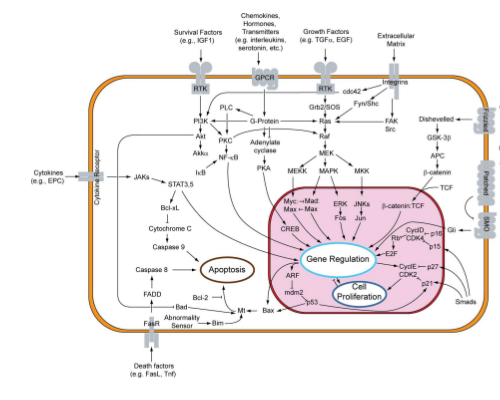
\includegraphics[scale=0.55]{images/cellule_description_lui.png}
% \end{center}
% \begin{center}
% {\tiny \color{darkgreen}[\citelui]}
% \end{center}
% 
% %\tcite{Wikipédia}
% 
% \begin{itemize}
% \item Cellular processes are driven by networks of biological interactions.
% \item Formal modelling and analysis of Biological Regulatory Network.
% \item Static analysis of properties.
% \end{itemize}
% 
% %Cellular processes are driven by networks of biological reactions. Cells rely on the tight coordination of these pathways to achieve proper functioning.
% %With the help of signaling pathway, a cell senses changes in its environnement or internal state. This information is then passed on via cascades of biochemical 
% %reactions to the appropriate mechanisms which respond by modifying the metabolic and transcriptiona activities. this in turn modifies the behavior of the cell.
% 
% %Consequently, the dynamics of biopathways play a crucial role in determinig cellular functions.
% 
% %Examples: circadian rhythm, the apoptosis pathway inducing programmed cell death, cell differentiation.
% 
% %\textcolor{couleurtheme}{$\Rightarrow$} \fbox{\tval{\large The need of comprehension of biological systems}} \textcolor{couleurtheme}{$\Leftarrow$}
% 
% 
% %\textcolor{couleurtheme}{$\Rightarrow$} \fbox{\tval{\large Allow efficient translation from Process Hitting to BRN}} \textcolor{couleurtheme}{$\Leftarrow$}
% 
% \end{frame}

\begin{frame}[c]
  \frametitle{Introduction à la notion de bifurcation}
 \framesubtitle{Différenciation des cellules souches}

\begin{center}
  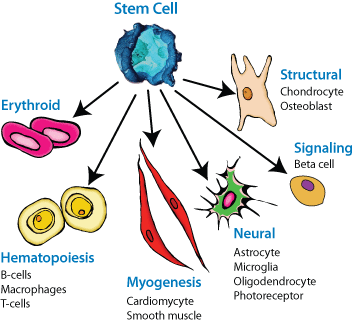
\includegraphics[scale=0.42]{images/illustration_differentiation.png}
  % \multiinclude[format=gif, scale=0.5]{images/illustration_differentiation.gif}
\end{center}
\begin{center}
{\tiny \color{darkgreen} [https://www.systembio.com/stem-cell-research/differentiation-reporters/overview]}
\end{center}
%\tcite{system Biosciences}

\begin{itemize}
\item \tval{Différenciation} $\Longrightarrow$ Perte de capacité %expliquer la notion de perte de capacité sur la figure.
\item Quelles transitions (opérations) sont responsables des \tval{bifurcations} ? 
\item \`A partir de quels états ?
\end{itemize}
\end{frame}

\begin{frame}[c]
  \frametitle{Approximation des bifurcations}
%system dynamique
%Bifurcations
%rajouter une autre image pour illustrer pour qu'on voit que c'est toujours des états qui changes
% \begin{center}
%   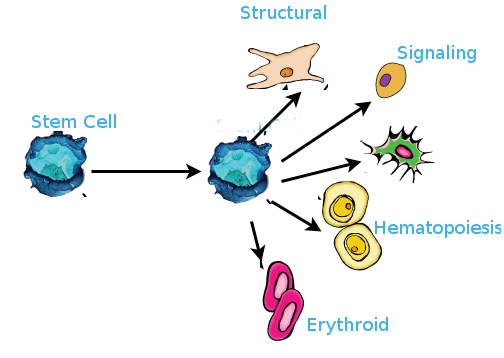
\includegraphics[scale=0.3]{images/illustration_differentiation_newio1.png}
%   % \multiinclude[format=gif, scale=0.5]{images/illustration_differentiation.gif}
% \end{center}
\begin{center}
\begin{tikzpicture}
 \node[esdef] (bif ) at (0,1) {\begin{tabular}{c} Bifurcations \\ \textcolor{red}{PSPACE Complet} \end{tabular}};
 
 \node[esdef] (bifctl) at (0,-2) {\begin{tabular}{c}$EF \ g_1  \wedge \cdots$  \\ (CTL) \end{tabular}};
 
 \node[esdef] (pl) at (6,-2) {\begin{tabular}{c}Programme logique \\ (SAT/ASP) \end{tabular}};
 
 \node[esdef] (abif) at (6,1) {\begin{tabular}{c}Approximation \\ des bifurcations \end{tabular}};
                                                                                  
 
  
 \draw[->] (bif) -- (bifctl);
 \draw[->] (bifctl)-- node[below=5pt,midway]{\textcolor{black}{\textbf{Approximation}}}node[above=5pt,midway]{\textcolor{black}{\textbf{IA + PL}}} (pl);
 \draw[->] (pl) -- (abif);
 
\end{tikzpicture}
\end{center}


\begin{liste}
%\item Les transitions de bifurcation peuvent être exprimées dans la logique temporelle
%\item {\bf "Approximation"} :\\ vérification d'une formule CTL (\tval{PSPACE (complet)})\\
%       $\Rightarrow$ Problème NP qui peut être aisément exprimé en SAT/ASP %trouver l'orthagraphe de easely
\item {\bf Contribution} : $$
\left\{
    \begin{array}{lcl}
        \mbox{PL (Programmation logique)} &\\  %rajouter un signe entre les deux
        \mbox{+} & \Longrightarrow \mbox{\tval{approximations formelles des bifurcations}} \\
        \mbox{IA (Interprétation abstraite)} &
    \end{array}
\right.
$$ 
\end{liste}
\end{frame}

 \subsection{C'est quoi une  bifurcation?}
 \begin{frame}[c]
 \frametitle{Illustration des bifurcations}
 
%\ref{ex-bifurcations} shows all the possible transitions from $s_0$.
\begin{figure}[p]
\centering

\scalebox{0.4}{

\begin{tikzpicture}[line join=bevel,font=\LARGE]
%%
  \node (6) at (405.0bp,18.0bp) [reach] {$\langle \mathbf{\color{blue}a_2},b_1,c_0\rangle$};
  \node (2) at (405.0bp,90.0bp) [reach] {$\langle \mathbf{\color{blue}a_2},b_0,c_0\rangle$};

\node (1) at (570.0bp,90.0bp) [reach] {$\langle a_1,b_0,c_0\rangle$};
  \node (64) at (304.0bp,234.0bp) [reach] {$\langle a_0,b_0,c_1\rangle$};
  \node (0) at (469.0bp,162.0bp) [reach] {$\langle a_0,b_0,c_0\rangle}$};
  \node (5) at (507.0bp,306.0bp) [reach] {$\langle a_1,b_1,c_0\rangle$};
  \node (4) at (469.0bp,234.0bp) [reach] {$\langle a_0,b_1,c_0\rangle$};
  \node (69) at (425.0bp,378.0bp) [reach] {$\mathbf{\color{Maroon}s_0 = \langle a_1,b_1,c_1\rangle$};
  \node (68) at (342.0bp,306.0bp) [reach] {$\langle a_0,b_1,c_1\rangle$};
  \node (65) at (232.0bp,450.0bp) [reach] {$\langle a_1,b_0,c_1\rangle$};

  \node[elipse,fill=gray!30] (129) at (88.0bp,90.0bp)  {$\langle a_1,b_0,c_2\rangle$};
  \node[elipse,fill=gray!30] (128) at (139.0bp,162.0bp)  {$\langle a_0,b_0,c_2\rangle$};
  \node[elipse,fill=gray!30] (133) at (112.0bp,306.0bp)  {$\langle a_1,b_1,c_2\rangle$};
  \node[elipse,fill=gray!30] (132) at (139.0bp,234.0bp)  {$\langle a_0,b_1,c_2\rangle$};

  \draw [->] (0) ..controls (445.65bp,135.46bp) and (435.95bp,124.86bp)  .. (2);
  \draw [->] (133) ..controls (121.57bp,280.18bp) and (125.26bp,270.62bp)  .. (132);
  \draw [->,very thick,red] (65) ..controls (104.12bp,424.19bp) and (0.0bp,387.99bp)  ..  (0.0bp,307.0bp) .. controls (0.0bp,307.0bp) and (0.0bp,307.0bp)  ..  node[auto,font=\huge,fill=white]{$t_8$} (0.0bp,233.0bp) .. controls (0.0bp,185.75bp) and (35.64bp,141.13bp)  .. (129);
  \draw [->] (65) ..controls (223.97bp,401.24bp) and (228.52bp,336.68bp)  .. (251.0bp,288.0bp) .. controls (255.96bp,277.25bp) and (263.67bp,266.89bp)  .. (64);
  \draw [->] (5) ..controls (483.32bp,333.07bp) and (470.02bp,344.55bp)  .. (69);
  \draw [->,very thick,red] (64) ..controls (244.15bp,207.61bp) and (210.57bp,193.36bp)  .. node[auto,font=\huge,fill=white]{$t_8$} (128);
  \draw [->] (5) ..controls (493.43bp,280.01bp) and (488.11bp,270.2bp)  .. (4);
  \draw [->] (0) ..controls (475.71bp,188.03bp) and (475.94bp,197.36bp)  .. (4);
  \draw [->] (1) ..controls (588.79bp,134.38bp) and (608.0bp,186.55bp)  .. (608.0bp,233.0bp) .. controls (608.0bp,307.0bp) and (608.0bp,307.0bp)  .. (608.0bp,307.0bp) .. controls (608.0bp,366.83bp) and (560.73bp,369.68bp)  .. (507.0bp,396.0bp) .. controls (446.14bp,425.81bp) and (370.03bp,438.87bp)  .. (65);
  \draw [->] (1) ..controls (572.33bp,138.66bp) and (571.97bp,203.11bp)  .. (551.0bp,252.0bp) .. controls (546.57bp,262.33bp) and (539.46bp,272.21bp)  .. (5);
  \draw [->] (129) ..controls (68.077bp,117.99bp) and (60.513bp,131.04bp)  .. (57.0bp,144.0bp) .. controls (44.446bp,190.33bp) and (38.221bp,207.83bp)  .. (57.0bp,252.0bp) .. controls (61.945bp,263.63bp) and (70.831bp,273.95bp)  .. (133);
  \draw [->] (128) ..controls (145.71bp,188.03bp) and (145.94bp,197.36bp)  .. (132);
  \draw [->] (69) ..controls (448.8bp,350.83bp) and (462.16bp,339.29bp)  .. (5);
  \draw [->] (2) ..controls (405.0bp,63.983bp) and (405.0bp,54.712bp)  .. (6);
  \draw [->] (0) ..controls (499.93bp,134.79bp) and (517.41bp,122.58bp)  .. (1);
  \draw [->] (68) ..controls (388.56bp,279.34bp) and (412.1bp,266.36bp)  .. (4);
  \draw [->] (68) ..controls (321.75bp,280.09bp) and (316.27bp,270.41bp)  .. (64);
  \draw [->] (1) ..controls (539.0bp,117.26bp) and (521.52bp,129.47bp)  .. (0);
  \draw [->] (65) ..controls (301.71bp,423.72bp) and (343.47bp,408.57bp)  .. (69);
  \draw [->] (64) ..controls (324.32bp,260.04bp) and (329.77bp,269.67bp)  .. (68);
  \draw [->] (69) ..controls (394.58bp,351.34bp) and (381.1bp,339.97bp)  .. (68);
  \draw [->] (128) ..controls (114.09bp,136.08bp) and (106.38bp,125.8bp)  .. (129);
  \draw [->] (64) ..controls (285.73bp,261.68bp) and (275.22bp,274.54bp)  .. (269.0bp,288.0bp) .. controls (248.81bp,331.74bp) and (243.08bp,388.29bp)  .. (65);
  \draw [->] (132) ..controls (132.3bp,208.35bp) and (132.06bp,199.03bp)  .. (128);
  \draw [->] (4) ..controls (462.3bp,208.35bp) and (462.06bp,199.03bp)  .. (0);
  \draw [->] (129) ..controls (113.05bp,116.11bp) and (120.71bp,126.32bp)  .. (128);
%
\end{tikzpicture}


}

%rajouter que quand on a jouer t8 on ne peut plus atteindre a2
%mettre s0 en évidence en gras ou vert 

%\caption{Transition graph of a given AN  from the initial state
%$s_0=\state{a_0,b_0,c_0}$. The goal $a_2$ is in thick/blue; the states connected to the goal are in
%gray; the bifurcations to the goal in thick/red, labelled with the local transitions in the AN definition.}
\label{ex-bifurcations}
\end{figure}

\end{frame}

 \begin{frame}
\frametitle{Définition d'une bifurcation}
\begin{figure}[t]
\centering
\begin{tikzpicture}[node distance=1.5cm]
\node (s0) [circle,fill=gray!60] {$s_0$};
\node (sb) [circle,fill=gray!60,above right of=s0,xshift=2cm] {$s_b$};
\node (g) [circle,fill=blue!20,minimum width=7mm,below right of=sb,xshift=2cm] {$g_1$};
\node (su) [above right of=sb] {$s_u$};
\node (u) [below right of=su,xshift=5mm] {};
\path[->] (sb) edge[->,red,thick] node[auto] {$t_b$} (su) ;
\path[->,bend left=20,densely dashed]
        (s0) edge (sb)
        (sb) edge (g)
        (s0) edge [bend right=10] (g)
        (su) edge[>={Rays[length=3mm,width=3mm,red]}] (u)
;
\end{tikzpicture}
\end{figure}

\begin{block}{Définition}
\centering
$t_b$ est une transition de bifurcation depuis $s_0$ pour $g_1$

\smallskip
$\Longleftrightarrow$
s'il existe $s_b$ tels que:
%rajouter g1 \in Sg
\begin{align*}
\text{\cI}\enspace &s_u\nreach g_1
&
\text{\cII}\enspace &s_b\reach g_1
&
\text{\cIII}\enspace &s_0\reach s_b
\end{align*}
\end{block}
\end{frame}

 \subsection{Comment identifier les bifurcations?}
 \begin{frame}[c]
 \frametitle{Approximation formelle de l'accessibilité}
\framesubtitle{Analyse statique par interprétation abstraite}
 
Les approximations pour l'accessibilité dans les AN\\
%\tcite{PMR12-MSCS,FPMR15-TCS}.
{\small \color{darkgreen} [\citepmrmscs] }%revoir les citations


 %\tval{over-approximations} (OA) and \tval{under-approximations} (UA) of the reachability problem:
$$
%\begin{align*}
\UA s {s'}&\Rightarrow {\bf s\reach s'} \Rightarrow \OA s {s'}
%\end{align*}
$$
\begin{itemize}
\item OA (\tval{sur-approximations}): conditions nécessaires pour {\bf $s\reach s'$} %is true only if $\OA s {s'}$ is true
\item UA (\tval{sous-approximation}): conditions suffisantes pour {\bf $s\reach s'$} %is true if  $\UA s {s'}$ is true;
\end{itemize}
\bigskip
\tval{Intérêt:}
\begin{itemize}
\item \'Eviter l'explosion de l'espace d'états
\item Décider de façon efficace les propriétés d'accessibilité
\end{itemize}

\end{frame}


\begin{comment}
\begin{frame}[c]
\frametitle{Formal approximation of reachability}
\framesubtitle{Local Causality Graph}
\begin{columns}
\begin{column}{0.5\textwidth}
\textbf{Idea for OA and UA}
\begin{itemize}
\item Local Causality reasonning
\item \tval{Nodes of LCG}: local states, objectives, solutions. 
\end{itemize}

\textbf {Sufficient condition}:
\begin{itemize}
\item LCG has \tval{no cycle};
\item each objective has \tval{at least one solution};
\item local states of a same pre-condition have no conflicts.
\end{itemize}

\end{column}
\begin{column}{0.5\textwidth}
%presentation of the GLC
  \begin{figure}[h]
 % \scalebox{0.5}{\begin{tikzpicture}[>={Stealth[width=3mm,length=3mm]},line join=bevel,font=\Large]
%%
\node (a_2) at (65.597bp,320.0bp) [draw,rectangle] {$a_2$};
  \node (O_b_0_0) at (28.597bp,61.0bp)  {$\anobj b 0 0$};
  \node (O_c_2_0) at (103.6bp,61.0bp)  {$\anobj c 2 0$};
  \node (c_0) at (102.6bp,133.0bp) [draw,rectangle] {$c_0$};
  \node (O_a_1_2) at (65.597bp,248.0bp)  {$\anobj a 1 2$};
  \node (b_0) at (29.597bp,133.0bp) [draw,rectangle] {$b_0$};
  \node (pintsol1) at (65.597bp,190.5bp) [draw,ellipse] {};
  \node (pintsol2) at (28.597bp,3.5bp) [draw,ellipse] {};
  \draw [->] (O_a_1_2) ..controls (65.597bp,221.59bp) and (65.597bp,212.02bp)  .. (pintsol1);
  \draw [->] (O_b_0_0) ..controls (28.597bp,34.59bp) and (28.597bp,25.018bp)  .. (pintsol2);
  \draw [->] (a_2) ..controls (65.597bp,293.98bp) and (65.597bp,284.71bp)  .. (O_a_1_2);
  \draw [->] (c_0) ..controls (102.95bp,106.98bp) and (103.09bp,97.712bp)  .. (O_c_2_0);
  \draw [->] (pintsol1) ..controls (70.418bp,182.27bp) and (78.07bp,170.79bp)  .. (c_0);
  \draw [->] (b_0) ..controls (29.24bp,106.98bp) and (29.108bp,97.712bp)  .. (O_b_0_0);
  \draw [->] (pintsol1) ..controls (60.907bp,182.27bp) and (53.462bp,170.79bp)  .. (b_0);
%
\end{tikzpicture}
}
  %\hfill
  \scalebox{0.3}{\begin{tikzpicture}[>={Stealth[width=3mm,length=3mm]},line join=bevel,font=\Large]
%%
\node (O_c_1_0) at (103.6bp,248.0bp)  {$\anobj c 1 0$};
  \node (a_2) at (65.597bp,507.0bp) [draw,rectangle] {$a_2$};
  \node (O_b_0_1) at (103.6bp,61.0bp)  {$\anobj b 0 1$};
  \node (O_b_0_0) at (28.597bp,248.0bp)  {$\anobj b 0 0$};
  \node (c_0) at (102.6bp,320.0bp) [draw,rectangle] {$c_0$};
  \node (O_a_1_2) at (65.597bp,435.0bp)  {$\anobj a 1 2$};
  \node (pintsol4) at (103.6bp,190.5bp) [draw,circle] {};
  \node (b_0) at (29.597bp,320.0bp) [draw,rectangle] {$b_0$};
  \node (b_1) at (103.6bp,133.0bp) [draw,rectangle] {$b_1$};
  \node (pintsol1) at (65.597bp,377.5bp) [draw,circle] {};
  \node (pintsol3) at (103.6bp,3.5bp) [draw,circle] {};
  \node (pintsol2) at (28.597bp,190.5bp) [draw,circle] {};
  \draw [->] (b_1) ..controls (103.6bp,106.98bp) and (103.6bp,97.712bp)  .. (O_b_0_1);
  \draw [->] (O_b_0_1) ..controls (103.6bp,34.59bp) and (103.6bp,25.018bp)  .. (pintsol3);
  \draw [->] (O_a_1_2) ..controls (65.597bp,408.59bp) and (65.597bp,399.02bp)  .. (pintsol1);
  \draw [->] (O_b_0_0) ..controls (28.597bp,221.59bp) and (28.597bp,212.02bp)  .. (pintsol2);
  \draw [->] (pintsol4) ..controls (103.6bp,182.05bp) and (103.6bp,171.59bp)  .. (b_1);
  \draw [->] (a_2) ..controls (65.597bp,480.98bp) and (65.597bp,471.71bp)  .. (O_a_1_2);
  \draw [->] (c_0) ..controls (102.95bp,293.98bp) and (103.09bp,284.71bp)  .. (O_c_1_0);
  \draw [->] (O_c_1_0) ..controls (103.6bp,221.59bp) and (103.6bp,212.02bp)  .. (pintsol4);
  \draw [->] (pintsol1) ..controls (70.418bp,369.27bp) and (78.07bp,357.79bp)  .. (c_0);
  \draw [->] (b_0) ..controls (29.24bp,293.98bp) and (29.108bp,284.71bp)  .. (O_b_0_0);
  \draw [->] (pintsol1) ..controls (60.907bp,369.27bp) and (53.462bp,357.79bp)  .. (b_0);
%
\end{tikzpicture}

}
  \hfill
  \scalebox{0.3}{
\begin{tikzpicture}[>={Stealth[width=3mm,length=3mm]},line join=bevel,font=\Large]
%%
\node (a_2) at (140.6bp,550.0bp) [draw,rectangle] {$a_2$};
  \node (a_0) at (28.597bp,133.0bp) [draw,rectangle] {$a_0$};
  \node (c_0) at (178.6bp,320.0bp) [draw,rectangle] {$c_0$};
  \node (O_b_1_0) at (28.597bp,248.0bp)  {$\anobj b 1 0$};
  \node (O_c_1_0) at (178.6bp,248.0bp)  {$\anobj c 1 0$};
  \node (b_0) at (103.6bp,320.0bp) [draw,rectangle] {$b_0$};
  \node (b_1) at (178.6bp,133.0bp) [draw,rectangle] {$b_1$};
  \node (O_b_0_1) at (140.6bp,61.0bp)  {$\anobj b 0 1$};
  \node (O_b_0_0) at (103.6bp,248.0bp)  {$\anobj b 0 0$};
  \node (pintsol8) at (215.6bp,3.5bp) [draw,ellipse] {};
  \node (pintsync1) at (140.6bp,377.5bp) [draw,regular polygon, regular polygon sides=4] {};
  \node (pintsol5) at (28.597bp,190.5bp) [draw,ellipse] {};
  \node (pintsol4) at (140.6bp,3.5bp) [draw,ellipse] {};
  \node (pintsol7) at (253.6bp,190.5bp) [draw,ellipse] {};
  \node (pintsol6) at (178.6bp,190.5bp) [draw,ellipse] {};
  \node (pintsol1) at (28.597bp,3.5bp) [draw,ellipse] {};
  \node (pintsol3) at (103.6bp,190.5bp) [draw,ellipse] {};
  \node (pintsol2) at (140.6bp,420.5bp) [draw,ellipse] {};
  \node (O_a_0_0) at (28.597bp,61.0bp)  {$\anobj a 0 0$};
  \node (b00) at (215.6bp,61.0bp)  {$\anobj b 1 1$};
  \node (c00) at (253.6bp,248.0bp)  {$\anobj c 0 0$};
  \node (O_a_0_2) at (140.6bp,478.0bp)  {$\anobj a 0 2$};
 % \node (root) at (140.6bp,622.0bp) [draw,draw=none] {root};
 % \draw [->] (root) ..controls (140.6bp,595.98bp) and (140.6bp,586.71bp)  .. (a_2);
  \draw [->] (b_1) ..controls (192.06bp,106.52bp) and (197.31bp,96.603bp)  .. (b00);
  \draw [->] (pintsol5) ..controls (28.597bp,182.05bp) and (28.597bp,171.59bp)  .. (a_0);
  \draw [->] (O_c_1_0) ..controls (178.6bp,221.59bp) and (178.6bp,212.02bp)  .. (pintsol6);
  \draw [->] (b_0) ..controls (74.866bp,292.18bp) and (62.137bp,280.3bp)  .. (O_b_1_0);
  \draw [->] (O_b_1_0) ..controls (28.597bp,221.59bp) and (28.597bp,212.02bp)  .. (pintsol5);
  \draw [->] (a_2) ..controls (140.6bp,523.98bp) and (140.6bp,514.71bp)  .. (O_a_0_2);
  \draw [->] (b_0) ..controls (103.6bp,293.98bp) and (103.6bp,284.71bp)  .. (O_b_0_0);
  \draw [->] (b_1) ..controls (164.7bp,106.4bp) and (159.22bp,96.311bp)  .. (O_b_0_1);
  \draw [->] (c_0) ..controls (178.6bp,293.98bp) and (178.6bp,284.71bp)  .. (O_c_1_0);
  \draw [->] (O_b_0_0) ..controls (103.6bp,221.59bp) and (103.6bp,212.02bp)  .. (pintsol3);
  \draw [->] (O_a_0_0) ..controls (28.597bp,34.59bp) and (28.597bp,25.018bp)  .. (pintsol1);
  \draw [->] (pintsol6) ..controls (178.6bp,182.05bp) and (178.6bp,171.59bp)  .. (b_1);
  \draw [->] (a_0) ..controls (28.597bp,106.98bp) and (28.597bp,97.712bp)  .. (O_a_0_0);
  \draw [->] (c00) ..controls (253.6bp,221.59bp) and (253.6bp,212.02bp)  .. (pintsol7);
  \draw [->] (c_0) ..controls (207.33bp,292.18bp) and (220.06bp,280.3bp)  .. (c00);
  \draw [->] (pintsync1) ..controls (135.46bp,368.8bp) and (127.92bp,357.48bp)  .. (b_0);
  \draw [->] (pintsync1) ..controls (145.87bp,368.8bp) and (153.62bp,357.48bp)  .. (c_0);
  \draw [->] (O_b_0_1) ..controls (140.6bp,34.59bp) and (140.6bp,25.018bp)  .. (pintsol4);
  \draw [->] (O_a_0_2) ..controls (140.6bp,451.59bp) and (140.6bp,442.02bp)  .. (pintsol2);
  \draw [->] (b00) ..controls (215.6bp,34.59bp) and (215.6bp,25.018bp)  .. (pintsol8);
  \draw [->] (pintsol2) ..controls (140.6bp,411.71bp) and (140.6bp,400.36bp)  .. (pintsync1);
%
\end{tikzpicture}

}
  \caption{\tiny
  (left) \tval{OA($\state{a_1,b_0,c_1}$,$a_2$)}  
  (right) \tval{UA($\state{a_0,b_1,c_1}$,$a_2$)} 
  }
  \end{figure}
\end{column}
\end{columns}
\end{frame}
\end{comment}


 %\input{parts/bif_tools_fr.tex}
 
\begin{frame}[c]
\frametitle{Relaxation du problème de l'identification des bifurcations}

\begin{figure}[t]
%\centering
\scalebox{0.6}{
\begin{tikzpicture}[node distance=1.5cm,left]
\node (s0) [circle,fill=gray!60] {$s_0$};
\node (sb) [circle,fill=gray!60,above right of=s0,xshift=2cm] {$s_b$};
\node (g) [circle,fill=blue!20,minimum width=7mm,below right of=sb,xshift=2cm] {$g_1$};
\node (su) [above right of=sb] {$s_u$};
\node (u) [below right of=su,xshift=5mm] {};
\path[->] (sb) edge[->,red,thick] node[auto] {$t_b$} (su) ;
\path[->,bend left=20,densely dashed]
        (s0) edge (sb)
        (sb) edge (g)
        (s0) edge [bend right=10] (g)
        (su) edge[>={Rays[length=3mm,width=3mm,red]}] (u)
;
\end{tikzpicture}
}
\end{figure}

{\color{magenta}{\#}}: conditions suffisantes.
\pause
\begin{align*}
\text{\cI}\enspace &s_b\play t_b\nreach g_1
&
\text{\iI}\enspace&\neg \OA{s_u}{g_1}
&
\text{\iI}&\Rightarrow\text{\cI}
\end{align*}

%rajouter sufficient condition/ précisier ce que veut dire sharp
%remplacer unf-prefix par reach.
\pause
\begin{align*}
\text{\cII}\enspace &s_b\reach g_1
&
\text{\iII}\enspace&\UA{s_b}{g_1}
&
\text{\iII}&\Rightarrow\text{\cII}
\end{align*}

\pause
\begin{align*}
\text{\cIII}\enspace &s_0\reach s_b
&
\begin{split}
\text{\iIIIa}\enspace&s_b\in\freach(s_0)\\
\text{\iIIIb}\enspace&\UA{s_0}{s_b}
\end{split}
&
\begin{split}
\text{\iIIIa}&\Leftrightarrow\text{\cIII}\\
\text{\iIIIb}&\Rightarrow\text{\cIII}
\end{split}
\end{align*}

\pause
\begin{align*}
\text{\iI} \ et\ \text{\iII}\ et \ (\text{\iIIIa} ou \text{\iIIIb}) \ \Rightarrow t_b\ est\ une\ bifurcation.
\end{align*}
\end{frame}



\begin{comment}
\begin{frame}[c]
 \frametitle{General scheme for identification of bifurcation}
%\framesubtitle{concepts and tools}
 
%A sound and complete characterization of the local transitions $t_b\in\anT$ triggering a bifurcation
%from state $s_0$ to the goal $g_1$ would be the following:
%$t_b$ is a bifurcation transition if and only if there exists a state $s_b\in\anS$ such that
\begin{align*}
\text{\cI}\enspace &s_b\play t_b\nreach g_1
&
\text{\cII}\enspace &s_b\reach g_1
&
\text{\cIII}\enspace &s_0\reach s_b
\end{align*}
%where $s_u = s_b\play t_b$, $s \nreach g_1 \EQDEF \forall s'\in\anS, s \reach s' \Rightarrow \get
%{s'}g\neq g_1$
%and $s\reach g_1\EQDEF \exists s_g\in\anS: \get{s_g}g = g_1\wedge s\reach s_g$.

%rajouter sufficient condition/ précisier ce que veut dire sharp
%remplacer unf-prefix par reach.

\begin{align*}
\text{\iI}\enspace&\neg \OA{s_u}{g_1}&
\text{\iII}\enspace&\UA{s_b}{g_1}&
\begin{split}
\text{\iIIIa}\enspace&s_b\in\unf(s_0)\\
\text{\iIIIb}\enspace&\UA{s_0}{s_b}
\end{split}
\end{align*}

%where $\unf(s_0)$ is the set of all reachable states from $s_0$ represented as the prefix of the
%unfolding of the AN which has to be pre-computed (\secref{unf}).
%Either \iIIIa or \iIIIb can be used, at discretion.
%From $\fOA$ and $\fUA$ properties (\secref{approx}), we directly obtain:
\begin{align*}
\text{\iI}&\Rightarrow\text{\cI}&
\text{\iII}&\Rightarrow\text{\cII}&
\begin{split}
\text{\iIIIa}&\Leftrightarrow\text{\cIII}\\
\text{\iIIIb}&\Rightarrow\text{\cIII}
\end{split}
\end{align*}

\begin{align*}
\text{\iI} \ and\ \text{\iII}\ and \ (\text{\iIIIa} or \text{\iIIIb}) \ \Rightarrow t_b\ is\ a\ bifurcation.
\end{align*}

\end{frame}
\end{comment}



\subsection{Mise en {\oe}uvre \& applications}
\begin{frame}[c]
\frametitle{Implémentation}
%\framesubtitle{Local Causality Graph}
\textbf{Approximations formelles de l'accéssibilité}
\begin{itemize}
\item Calcul du  \tval{Graphe de Causalité Locale}
\item OA/UA: motifs particuliers dans le GLC
\item Taille GLC: poly(\#automata),exp(|single automaton|)
\end{itemize}
\bigskip
\textbf{Implémentation en ASP (Answer Set Programming)}
\begin{itemize}
\item Modélisation du problème: trouver $s_b$, $t_b$ tels que
\begin{align*}
{\color{magenta} \neg \OA{s_b \cdot t_b}{g_1}} \ et\ {\color{magenta}\UA{s_b}{g_1}}\ et \  {\color{magenta}\UA{s_0}{s_b}}
\end{align*}
\item \'Enumération  avec  clingo
\end{itemize}
\end{frame}

\subsection{Applications biologiques de l'identification des bifurcations}
 
\begin{frame}[c]
 \frametitle{Cas d'étude}
 

\tval{Phage Lambda} : ($4$  composants et $11$  interactions); 

\tval{EGF/TNF} : ($28$  composants et $55$  interactions); 

\tval{t\_helper differentiation}: ($101$  composants et $381$  interactions).

\begin{center}
  \includegraphics[scale=0.18,angle=-90]{images/th_differentiation.jpg}
\end{center}
\begin{center}
 {\tiny \color{darkgreen} [\citeatfb]}
\end{center}
\end{frame}



%mettre le tableau
\begin{frame}[c]
 \frametitle{Résultats de l'identification des bifurcations}
 

%mettre le tableau
\begin{table}[bt]
\renewcommand{\arraystretch}{1.3}

\centering
%table of result
\scalebox{0.8}{
\setlength{\tabcolsep}{2mm}
\begin{tabular}{|c|c||c|r||c|r||c|r|}
\hline
\multirow{2}{*}{Automata Network} 
& \multirow{2}{*}{Goal}
& \multicolumn{2}{c||}{M-C (NuSMV)}
& \multicolumn{2}{c||}{avec \iIIIa}
& \multicolumn{2}{c|}{avec \iIIIb}
\\
\cline{3-8}
&&$\card{t_b}$&Time&$\card{t_b}$&Time&$\card{t_b}$&Time
\\\hline

Lambda phage &  $\mathrm{CI}_2$ & $10$ & $0.1s$ & $6$ & $0.1s$ & $0$ & $0.2s$ 	
\\
$\card\anN=4\quad\card\anT=11$ &$\mathrm{Cro}_2$ & $3$ & $0.1s$ & $3$ & $0.1s$ & $2$ & $0.3s$ 	
\\ \hline 

EGF/TNF       & $\mathrm{NFkB}_0$ & $5$ & $0.2s$ & $4$ & $0.1s$ & $2$ & $0.1s$ 
\\

$\card\anN=28\quad\card\anT=55$ & $\mathrm{IKB}_1$ & $5$ & $0.2s$ & $3$ & $0.1s$ & $2$ & $0.1s$ 

\\ \hline

Th\_th17 & $\mathrm{RORGT}_1$ & $18$ & $48s$ & $9$ & $23s$ & $8$ & $26s$  
\\
$\card\anN=101\quad\card\anT=381$ & $\mathrm{BCL6}_1$ &$7$ & $26s$ &$5$ & $23s$ & $4$ & $24s$ 

\\ \hline

Th\_HTG & $\mathrm{BCL6}_1$ & \multicolumn{2}{c||}{\multirow{2}{*}{$\geq 2h$}} & \multicolumn{2}{c||}{\multirow{2}{*}{$\geq 2h$}} & $6$ & $61s$ 

\\

$\card\anN=101\quad\card\anT=381$ & $\mathrm{GATA3}_1$ &  \multicolumn{2}{c||}{} &\multicolumn{2}{c||}{}  & $7$ & $34s$ 

\\ \hline



\end{tabular}
}
\end{table}
\begin{center} Implémenté en  ASP (Answer Set Programming) et avec clingo 4.5.4.\end{center}
\end{frame}

% \begin{frame}
% %mettre cette slide un peu avant la conclusion
% \frametitle{Automata Network modelling of Biological Networks}
% \textbf{Transition-centered specification}
% \begin{itemize}
% \item ...in opposition to function-centered of Boolean/Thomas networks
% \item explicit context/ \tval{causality of state changes}
% \item closely related to (safe) Petri nets
% \item step semantics (purely async, purely sync, mixed)
% \end{itemize}
% \textbf{Modelling}
% \begin{itemize}
% \item any Boolean/Thomas networks can be encoded;
% \item in case of logical rules uncertainty: \tval{model the union} of Boolean/Thomas networks (over-approximation of behaviours)
% %\item encoding of \tval{SBGN Process Description} models
% \end{itemize}
% \end{frame}

 \begin{frame}[c]
  \frametitle{Synthèse sur l'identification des bifurcations}

%mots clés: large scale
%bien expliquer les résultats obtenus
% \textbf{Summary}

%\pause
\tval{Approximations formelles des états et transitions de bifurcation}\\
\medskip
\textbf{Combinaison de deux abstractions}
  \begin{itemize}
   \item $$
\left\{
    \begin{array}{lcl}
        \mbox{PL (Programmation logique)} &\\  %rajouter un signe entre les deux
        \mbox{+} & \Rightarrow \mbox{\tval{approximations formelles des bifurcations}} \\
        \mbox{IA (Interprétation abstraite)} &
    \end{array}
\right.
$$
\item Applicable sur les grands modèles.
\item Manquer certaines bifurcations.
  \end{itemize}
\medskip
\textbf{Application sur des modèles biologiques réels}
\begin{itemize}
 \item Lambda phage, EGF/TNF, Différenciation des lymphocytes T.
 \item Base pour la reprogrammation cellulaire.
\end{itemize}
\medskip
\textbf{Publication}
\begin{itemize}
 \footnotesize
 \item
Louis Fippo Fitime, Olivier Roux, Carito Guziolowski, Loïc Paulevé. \tscite{Identification of Bifurcations in Biological
Regulatory Networks using Answer-Set
Programming}. In \textit{12th International Workshop on Constraint-Based Methods for Bioinformatics (WCB'12)}. September 2016.

\end{itemize}

\end{frame}
% %\subsection{Implementation}
% %\input{parts/bif_asp_implementation_fr.tex}
% 
 %
\begin{frame}[c]
 \frametitle{Applications biologiques}
 
 But: Montrer des applications concrètes pour la biologie des systèmes. 
 
 \medskip
 
 \textbf{Application de l'intégration des données}
 \begin{itemize}
  \item Hypothèses biologiques considérées \& choix des paramètres.
  \item Résultats des simulations des gènes et processus cellulaires.
  \item Analyse statistique des traces.
 \end{itemize}
 
 \medskip
\pause
\textbf{Identification des bifurcations}
\begin{itemize}
 \item Présentation des modèles biologiques.
 \item Résultats vs model-checking exact.
\end{itemize}

\end{frame}

%\begin{frame}[c]
 \frametitle{Applications biologiques}
 
 But: Montrer des applications concrètes pour la biologie des systèmes. 
 
 \medskip
 \pause
 \textbf{Application de l'intégration des données}
 \begin{itemize}
  \item Hypothèses biologiques considérées \& choix des paramètres.
  \item Résultats des simulations des gènes et processus cellulaires.
  \item Analyse statistique des traces.
 \end{itemize}
 
 \medskip
 \pause
\textbf{Identification des bifurcations}
\begin{itemize}
 \item Présentation des modèles biologiques.
 \item Résultats vs model-checking exact.
\end{itemize}

\end{frame}

\begin{frame}[c]
 \frametitle{Applications biologiques}
 
 But: Montrer des applications concrètes pour la biologie des systèmes. 
 
 \medskip
 
 \textbf{Application de l'intégration des données}
 \begin{itemize}
  \item Hypothèses biologiques considérées \& choix des paramètres.
  \item Résultats des simulations des gènes et processus cellulaires.
  \item Analyse statistique des traces.
 \end{itemize}
 
 \medskip
%  \uncover<2->{
% \textbf{Identification des bifurcations}
% \begin{itemize}
%  \item Présentation des modèles biologiques.
%  \item Résultats vs model-checking exact.
% \end{itemize}
% }
\end{frame}

 

% 
% 
% %%%%%%%    la conclusion
\section{Conclusions \& Perspectives}
 % Performances et conclusion
\begin{frame}[c]
  \frametitle{Conclusions}

%mots clés: large scale
%bien expliquer les résultats obtenus
% \textbf{Summary}
{\small
\pause
\textbf{Modélisation hybride des réseaux RSTC}
  \begin{itemize}
   \item Formalisation des connaissances biologiques: Translation des motifs en AN
   \item Inférence et intégration des paramètres temporels et stochastiques
   \item Raffinement qualitatif et quantitatif de la dynamique
  \end{itemize}
\pause
\textbf{Analyse statique des propriétés quantitatives (probabilité/délai)}
\begin{itemize}
 \item 
  $$
\left\{
    \begin{array}{lcl}
        \mbox{QS (Classes d'\'Equivalences d'\'Etats)} &\\  %rajouter un signe entre les deux
        \mbox{+} & \Longrightarrow \mbox{\tval{approximations formelles}} \\
        \mbox{IA (Interprétation Abstraite)} & \mbox{\tval{des propriétés quantitatives}}
    \end{array}
\right.
$$ 
 \item Estimation efficace d'une borne inférieure de la probabilité et du délai de l'accessibilité 
 \item Faible complexité théorique
\end{itemize}


\pause
\textbf{Identification des Bifurcations}
 \begin{itemize}
\item 
$$
\left\{
    \begin{array}{lcl}
        \mbox{PL (Programmation logique)} &\\  %rajouter un signe entre les deux
        \mbox{+} & \Longrightarrow \mbox{\tval{approximation formelle des bifurcations}} \\
        \mbox{IA (Interprétation abstraite)} &
    \end{array}
\right.
$$ 
   \item Applicable aux grands modèles  (vs model-checking)
  % \item Sous-approximation: possible de manquer certaines bifurcations.
   %\item Application on \tval{Phage lambda, EGF/TNF, Th\_differentiation} 
  \end{itemize}
\medskip
}
\end{frame}

%rajouter les slides du titre




 \begin{frame}
 \frametitle{Perspectives}
 \pause
 \textbf{Simulation stochastique \& de l'analyse statique des traces}
 \begin{itemize}
  \item Analyse statistique qui prenne en compte le temps.
  \item Utilisation des règles d'associations pour identifier les relations non encore connues.
 \end{itemize}

 \pause
 \textbf{Analyse statique des propriétés quantitatives}
 \begin{itemize}
  \item Implémentation (en cours...) d'un analyseur statique des propriétés (CCSL Logic)
  \item Analyse statique des comportements à long terme (états stables)
  \item Analyse statique des modèles paramétriques
 \end{itemize}

 \pause
 \textbf{Identification des Bifurcations}
 \begin{itemize}
%parler d'améliorer les conditions initiales
  \item Sur-approximation des bifurcations
  %\item Frame the number of attractors
  \item Utilisation des bifurcations pour l'analyse des probabilités 
  \item Applications pour \tval{prédire les cibles pour la reprogrammation cellulaire.}
  
 \end{itemize}
%\medskip

 
 
%  \begin{block}{Formal verification of quantitative properties and key process (in progress)}
%   \begin{itemize}
%    \item Static analysis of quantitative properties of reachability in Asynchronous automata networks
%    \item Logical verification and key processes detection
%    \item Experimental validation of in silico hypotesis
%    %\item Integrate de likelihood in the parameters estimation procedure.
%   \end{itemize}
% 
%  \end{block}
%  
%  \begin{block}{Association rules and traces in automata networks}
%   \begin{itemize}
%    \item Association rules for discovering interesting relations between local states. 
%    \item Experimental validation of in silico hypotesis
%   \end{itemize}
% 
%  \end{block}
 
\end{frame}







\begin{frame}[plain,label=title]

% Cadre de titre
\begin{center}
\vspace{1cm}
\setbeamercolor{postit}{fg=black,bg=colortitle}
\begin{beamercolorbox}[sep=0.5em]{postit}
\centering
\Large
\textbf{%
{\normalsize\theconference{}}\\~\\%
\inserttitle
}
\end{beamercolorbox}

% Auteurs et instituts
% Auteurs et instituts
\par
\medskip
\normalsize
Louis Fippo Fitime
\footnotesize

\texttt{louis.fippo-fitime@irccyn.ec-nantes.fr}

%\url{http://www.irccyn.ec-nantes.fr/~folschet/}

\normalsize
\bigskip
Lundi 28 novembre 2016

\medskip

{\scriptsize
\begin{tabular}{rl}
\textbf{Rapporteurs:} & Christine FROIDEVAUX, Professeur des universités, Université Paris Sud\\
                      & Simon de GIVRY, Chargé de recherche INRA, INRA Toulouse \\
\textbf{Examinateurs:} & Anne POUPON, Directrice de recherche CNRS, INRA de Tours\\
                      & Sylvain SOLIMAN, Chargé de recherche INRIA, INRIA Paris Saclay\\
                       
\textbf{Directeur de thèse:} & Olivier ROUX, Professeur des universités, \'Ecole centrale de Nantes\\
\textbf{Co-encadrant de thèse:} & Carito GUZIOLOWSKI, Maître de conférences, \'Ecole centrale de Nantes\\

\end{tabular}
}

\end{center}
\medskip
{\centering
Merci de votre attention!
}
\end{frame}




%%%%%% appendix and bibliographie
%\appendix
%\section[x]{Bibliography}
%% Bibliographie

\begin{frame}[c]
  \frametitle{Bibliography}

\footnotesize
\setlength{\parindent}{-1em}
\setlength{\parskip}{0.5em}
~

\vfill
%\tcite{Paulevé11} Loïc Paulevé. PhD thesis: \textit{Modélisation, Simulation et Vérification des Grands Réseaux de Régulation Biologique}, October 2011, Nantes, France

\tcite{Paulev\'e et al. 2010} Loïc Paulevé, Morgan Magnin, and Olivier Roux. \textit{Tuning Temporal Features within the Stochastic $\pi$-Calculus}. IEEE Transactions on Software Engineering, 37(6):858-871, 2011.

%\tcite{PRM10-TCSB} Loïc Paulevé, Morgan Magnin, and Olivier Roux. \textit{Refining dynamics of gene regulatory networks in a stochastic $\pi$-calculus framework}. In Corrado Priami, Ralph-Johan Back, Ion Petre, and Erik de Vink, editors: Transactions on Computational Systems Biology XIII, volume 6575 of Lecture Notes in Computer Science, 171-191. Springer Berlin/Heidelberg, 2011.

\tcite{Paulev\'e et al. 2012} Loïc Paulevé, Morgan Magnin, and Olivier Roux. \textit{Static analysis of biological regulatory networks dynamics using abstract interpretation}. Mathematical Structures in Computer Science, in press, 2012.

%\tcite{PR10-CRAS} Loïc Paulevé and Adrien Richard. \textit{Topological Fixed Points in Boolean Networks}. Comptes Rendus de l'Académie des Sciences - Series I - Mathematics, 348(15-16):825 - 828, 2010.

\tcite{Richard et al. 2008} Adrien Richard, Jean-Paul Comet, and Gilles Bernot. \textit{R. Thomas' logical method}, 2008. Invited at Tutorials on modelling methods and tools: Modelling a genetic switch and Metabolic Networks, Spring School on Modelling Complex Biological Systems in the Context of Genomics.

%\tcite{CMSB12} Maxime Folschette, Loïc Paulevé, Katsumi Inoue, Morgan Magnin, and Olivier Roux. \textit{Concretizing the Process Hitting into Biological Regulatory Networks}. In: Computational Methods in Systems Biology, Springer, 2012.




\tcite{Ahmad et al. 2008}
Jamil Ahmad, Olivier Roux, Gilles Bernot, Jean-Paul Comet, and Adrien Richard.
\textit{Analysing formal models of genetic regulatory networks with delays.}
 International Journal of Bioinformatics Research and
  Applications (IJBRA), 4(3):240--262, 2008.

\tcite{Batt et al. 2007}
Gr{\'e}gory Batt, Ramzi~Ben Salah, and Oded Maler.
 \textit{On timed models of gene networks.}
 Springer, 2007.

\tcite{Gardner et al. 2003}
Timothy~S Gardner, Diego Di~Bernardo, David Lorenz, and James~J Collins.
 \textit{Inferring genetic networks and identifying compound mode of action
  via expression profiling.}
  Science, 301(5629):102--105, 2003.

\tcite{Guziolowski et al. 2012}
Carito Guziolowski, Aristotelis Kittas, Florian Dittmann, and Niels Grabe.
\textit{ Automatic generation of causal networks linking growth factor stimuli
  to functional cell state changes.}
 FEBS Journal, 279(18):3462--3474, 2012.

\tcite{Heiner et al. 2008}
Monika Heiner, David Gilbert, and Robin Donaldson.
 \textit{Petri nets for systems and synthetic biology.}
 Formal methods for computational systems biology, pages
  215--264. Springer, 2008.

\tcite{Mac Namara et al. 2012}
Aidan MacNamara, Camille Terfve, David Henriques, Beatriz~Pe{\~n}alver
  Bernab{\'e}, and Julio Saez-Rodriguez.
 \textit{State--time spectrum of signal transduction logic models.}
 Physical Biology, 9(4):045003, 2012.


\vfill
\Large
\begin{flushright}
  \tval{Thank you}\hspace{1cm}~
\end{flushright}
\vfill

~

\end{frame}



%%%%%% section annexe 
\section{Annexes}
\subsection{Sortes de synchronisation}
\begin{frame}
 \frametitle{Sortes de synchronisation}
 
 \begin{tabular}{|cc|}
\hline
\textbf{Motifs biologiques} &

\\ \hline

\begin{tikzpicture}
\node[scale=0.7] (sai1) at (0,0){\begin{tikzpicture}[auto]
\path[use as bounding box] (-0.7,-0.3) rectangle (2.5,3);
\node[qgre] (a) at (0,2) {a};
\node[mod] (i) at (1,1) {i};
\node[qgre] (b) at (0,0) {b};
\node[qgre] (c) at (2,1) {c};
\node[es] (d) at (1,2.5) {activations indep.};

% arestorer
\path
 (a) edge[act] (i)
 (b) edge[act] (i)
 (i) edge[st]  (c);
\end{tikzpicture}};
\end{tikzpicture}


&

\begin{tikzpicture}
\node[scale=0.7] (sai1) at (0,0){\begin{tikzpicture}[auto]
\path[use as bounding box] (-0.7,-0.3) rectangle (2.5,3);
\node[qgre] (a) at (0,2) {a};
\node[mod] (i) at (1,1) {i};
\node[qgre] (b) at (0,0) {b};
\node[qgre] (c) at (2,1) {c};
\node[es] (d) at (1,2.5) {inhibitions indep.};

% arestorer
\path
 (a) edge[inh] (i)
 (b) edge[inh] (i)
 (i) edge[st]  (c);
\end{tikzpicture}};
\end{tikzpicture}

\\ \hline

\end{tabular}
\end{frame}

\begin{frame}
  \frametitle{Sortes de synchronisation}
  \framesubtitle{Raffinement structurel de la dynamique}
  %\framesubtitle{\tcite{PMR12-MSCS}}


\scalebox{\scaleex}{
\begin{tikzpicture}
\exphsyn
\end{tikzpicture}
}

\only<-14>{
\begin{liste}
  \item Comment introduire la \tval{Synchronisation} entre les sortes? \qex{$\PHfrappe{a_0 \wedge b_0}{c_2}{c_1}$}
\end{liste}
}

\end{frame}

\begin{frame}
\frametitle{Résultat avec la synchronisation}
% \begin{columns}
%  \begin{column}{0.3\textwidth}
% \scalebox{0.8}{
% \begin{tikzpicture}
% 
%  \node[scale=0.3] (syn) at (0,0) {
%  \includegraphics{figs/synchronisation.png}
%  oscillation.png: 400x1000 pixel, 72dpi, 14.11x35.27 cm, bb=0 0 400 1000
% };
% \end{tikzpicture}
% }
% 
% \end{column}
% 
% \end{columns}

\begin{figure}[!h]
   \begin{minipage}[c]{.46\linewidth}
      \centering
      \includegraphics[scale=0.2]{figs/oscillation.png}
   \end{minipage} \hfill
   \begin{minipage}[c]{.46\linewidth}
   \centering
      \includegraphics[scale=0.2]{figs/synchronisation.png}
   \end{minipage}
\end{figure}

\end{frame}


\subsection{Formules générales pour le QGLC}
\begin{frame}
\frametitle{Graphe de causalité locale quantifié}

% \begin{columns}
%  \begin{column}{0.2\textwidth}
%   \begin{center}\scalebox{0.6}{
% \begin{tikzpicture}
% \exsanppdef
% \end{tikzpicture}
% }\end{center}
%  \end{column}
%  \begin{column}{0.8\textwidth}
 \begin{itemize}
  
 \item Probabilité d'un  \tval{n{\oe}ud état local}:\\
 $\GProbLS{\n}{\ctx}{\cwG}{k}$\\
 \medskip
 \pause
 \item Probabilité d'un  \tval{n{\oe}ud objectif}:\\
 $\GProbObjn{\n}{\ctx}{\cwG}{k}$\\
 \medskip
 \pause
 \item Probabilité d'un  \tval{n{\oe}ud Solution}:\\
 $\GProbSol{\n}{\ctx}{\cwG}{k}$
 \end{itemize}
 \pause
   \begin{center}\scalebox{\scaleex}{
    
    \exqlcggaidef
   
   }\end{center}
   
%  \end{column}
% \end{columns}


\end{frame}


\begin{comment}
plan pour la presentation de ma thèse

-introduction

-integration des données

-analyse statitique des propriétés quantitatives
  
  *probability in CTMC
  *

-analyse statique des bifurcations

-implementation

-biological applications



\end{comment}




\end{document}
